\documentclass[phd,electronic,oneside,twosidetoc,letterpaper,chaptercenter,parttop,lol,lof,lot]{byumsphd}
% Author: Paul Bodily
%
% This document is in the public domain
%
% Options for this class include the following (* indicates default):
%
%   phd (*) -- produce a dissertation
%   ms -- produce a thesis
%
%   electronic -- default official university option, overrides the following:
%                 - equalmargins
%
%   hardcopy -- overrides the following:
%                 - no equalmargins
%                 - twoside
%
%   letterpaper -- ignored, but helpful for the Makefile that I use
%
%   10pt -- 10 point font size
%   11pt -- 11 point font size
%   12pt (*) -- 12 point font size
%
%   lof -- produce a list of figures in the preamble (off)
%   lot -- produce a list of tables in the preamble (off)
%   lol -- produce a list of listings in the preamble (off)
%
%   layout -- show layout lines on the pages, helps with overfull boxes (off)
%   grid -- show a half-inch grid on every page, helps with printing (off)
%   separator -- print an extra instruction page between preamble and body (off)
%
%   twoside (*) -- two-sided output (margins alternate for odd and even pages,
%     blank pages inserted to ensure that chapters begin on the right side of a
%     bound copy, etc.)
%   oneside -- one-sided output (margins are the same on all pages)
%   equalmargins -- make all margins equal - ugly for binding, but compliant
%
%   twosidetoc - start two-sided margins at the TOC instead of the body.  This
%     is sometimes (oddly) required, but be aware that it will make the page
%     numbering seem screwy, e.g., the first four full sheets of paper will
%     have number i-iv (not shown, though), and the next sheets will each have
%     two numbers, one for each side.  I suspect that most people don't look at
%     the roman numerals anyway, but it is a weird requirement.
%
%   openright (*) -- force new chapters to start on an odd page
%   openany -- don't use this, it's ugly
%
%   prettyheadings -- make the section/chapter headings look nice
%   compliantheadings (*) -- make them look ugly, but compliant with standards
%
%   chaptercenter -- center the chapter headings horizontally
%   chapterleft (*) -- place chapter headings on the left
%
%   partmiddle -- Part headers are centered vertically, no other text on page
%   parttop (*) -- Part headers at top of page, other text expected
%
%   duplexprinter -- Ensures that the two-sided portion starts on the right
%     side when printing.  This is not for use in submission, since the best
%     thing to do there is to print everything out one-sided, then take it down
%     to the copy store to have them do the rest.  It does help to save trees
%     when you are printing out copies just to look at them and fiddle with
%     things.
%
%
% EXAMPLES:
%
% The rest is up to you.  To fiddle with margins, use the \settextwidth and
% \setbindingoffset macros, described below.  I suggest that you
% \settextwidth{6.0in} for better-looking output (otherwise you'll get 3/4-inch
% margins after binding, which is sort of weird).  This will depend on the
% opinions of the various dean/coordinator folks, though, so be sure to ask
% them before embarking on a major formatting task.

% The following command fixes my particular printer, which starts 0.03 inches
% too low, shifting the whole page down by that amount.  This shifts the
% document content up so that it comes out right when printed.
%
% Discovering this sort of behavior is best done by specifying the ``grid''
% option in the class parameters above.  It prints a 1/2 inch grid on every
% page.  You can then use a ruler to determine exactly what the printer is
% doing.
%
% Uncomment to shift content up (accounting for printer problems)
%\setlength{\voffset}{-.03in}

% Here we set things up for invisible hyperlinks in the document.  This makes
% the electronic version clickable without changing the way that the document
% prints.  It's useful, but optional.
%
% NOTE: "driverfallback=ps2pdf" chooses ps2pdf in the case of LaTeX and pdftex
% in the case of pdflatex. If you use my LaTeX makefile (at
% http://latex-makefile.googlecode.com/) then pdftex is the default There are
% many other benefits to using the makefile, too.  This option is not always
% available, so use with care.
\usepackage[
    bookmarks=true,
    bookmarksnumbered=true,
    breaklinks=false,
    raiselinks=true,
    pdfborder={0 0 0},
    colorlinks=false,
    plainpages=false,
    ]{hyperref}

% To fiddle with the margin settings use the below.  DO NOT change stuff
% directly (like setting \textwidth) - it will break subtle things and you'll
% be tearing your hair out.
%
% For example, if you want 1.5in equal margins, or 2in and 1in margins when
% printing, add the following below:
%
%\setbindingoffset{1.0in}
%\settextwidth{5.5in}
%
% When equalmargins is specified in the class options, the margins will be
% equal at 1.5in each: (8.5 - 5.5) / 2.  When equalmargins is not specified,
% the inner margin will be 2.0 and the outer margin will be 1.0: inner = (8.5 -
% 5.5 - 1.0) / 2 + 1.0 (the 1.0 is the binding offset).
%
% The idea is this: you determine how much space the text is going to take up,
% whether for an electronic document (equalmargins) or not.  You don't want the
% layout shifting around between printed and electronic documents.
%
% So, you specify the text width.  Then, if there is a binding offset (when
% binding your thesis, the binding takes up space - usually 0.5 inches), that
% reduces the visual space on the final printed copy.  So, the *effective*
% margins are calculated by reducing the page size by the binding offset, then
% computing the remaining space and dividing by two.  Adding back in the
% binding offset gives the inner margin.  The outer margin is just what's left.
%
% All of this is done using the geometry package, which should be manipulated
% directly at your peril.  It's best just to use the above macros to manipulate
% your margins.
%
% That said, using the geometry macro to set top and bottom margins, or
% anything else vertical, is perfectly safe and encouraged, e.g.,
%
%\geometry{top=2.0in,bottom=2.0in}
%
% Just don't fiddle with horizontal margins this way.  You have been warned.

% This makes hyperlinks point to the tops of figures, not their captions
\usepackage[all]{hypcap}

% These packages allow the bibliography to be sorted alphabetically and allow references to more than one paper to be sorted and compressed (i.e. instead of [5,2,4,6] you get [2,4-6])
\usepackage[numbers,sort&compress]{natbib}

% Because I use these things in more than one place, I created new commands for
% them.  I did not use \providecommand because I absolutely want LaTeX to error
% out if these already exist.
\newcommand{\Title}{Machine Learning for Inspired, Structured, Lyrical Music Composition}
\newcommand{\Author}{Paul M. Bodily}
\newcommand{\GraduationMonth}{August}
\newcommand{\GraduationYear}{2018}

% Set up the internal PDF information so that it becomes part of the document
% metadata.  The pdfinfo command will display this.
\hypersetup{%
    pdftitle=\Title,%
    pdfauthor=\Author,%
    pdfsubject={PhD Dissertation, BYU CS Department: %
                Degree Granted \GraduationMonth~\GraduationYear, Document Created \today},%
    pdfkeywords={Machine Learning, Markov Processes, Constraint Satisfaction, Computational Creativity},%
}

% Rewrite the itemize, description, and enumerate environments to have more
% reasonable spacing:
\newcommand{\ItemSep}{\itemsep 0pt}
\let\oldenum=\enumerate
\renewcommand{\enumerate}{\oldenum \ItemSep}
\let\olditem=\itemize
\renewcommand{\itemize}{\olditem \ItemSep}
\let\olddesc=\description
\renewcommand{\description}{\olddesc \ItemSep}

% Important settings for the byumsphd class.
\title{\Title}
\author{\Author}

\committeechair{Dan Ventura}
\committeemembera{Neil Thornock}
\committeememberb{Mark J. Clement}
\committeememberc{Jacob Crandall}
\committeememberd{Seth Holladay}

\yearcopyrighted{\GraduationYear}

\documentabstract{%
	Computational creativity has been called the ``final frontier'' of artificial intelligence due to the difficulty inherent in defining and implementing creativity in computational systems. Despite this difficulty computer creativity is becoming a more significant part of our everyday lives, in particular music. This is observed in the prevalence of music recommendation systems, co-creational music software packages, smart playlists, and procedurally-generated video games. Significant progress can be seen in the advances in industrial applications such as Spotify, Pandora, Apple Music, etc., but several problems persist. Of more general interest, however, is the question of whether or not computers can exhibit autonomous creativity in music composition. One of the primary challenges in this endeavor is enabling computational systems to create music that exhibits global \emph{structure}, that can \emph{learn} structure from data, and which can effectively incorporate autonomy and intention. 
	
	We seek to address these challenges in the context of a modular machine learning framework called hierarchical Bayesian program learning (HBPL). Breaking the problem of music composition into smaller pieces, we focus primarily on developing machine learning models that solve the problems related to structure. In particular we present an adaptation of non-homogenous Markov models that enable binary constraints and we present a structural learning model, the multiple Smith-Waterman (mSW) alignment method, which extends sequence alignment techniques from bioinformatics. To address the issue of intention, we incorporate our work on structured sequence generation into a full-fledged computational creative system called Pop* which we show through various evaluative means to possess to varying extents the characteristics of creativity and also creativity itself.
}

\documentkeywords{%
    Machine Learning, Markov Processes, Constraint Satisfaction, Computational Creativity
}

\acknowledgments{%

I could never have finished my PhD without the undying support of my wife, Courtney and our three children, Austin, Siena, and Autumn. I'll be forever indebted to a wife who believes whole-heartedly in the value of education and who was willing to settle for a student salary for the first 8 years of our marriage. She has sacrificed her own career and her own hobbies so that \emph{we} could earn a PhD. Though her name is not on the dissertation, the sacrifices that she made for this goal to be achieved were as numerous and significant as any I might have made. So congratulations, Courtney! We did it!

I approached Dr. Dan Ventura in the summer of 2015 about the possibility of doing a PhD in computational creativity. For me that was a big leap. I would have never found the faith and courage to do it if Dan had not believed in me. His optimism, charisma, and friendship have played a monumental role in my success and the vision that I have of my potential. More than investing in my PhD, he has invested in me and my future as a husband, a father, and a academician. Thank you, Dan.

I may well have never done a PhD at all were it not for Dr. Mark Clement. Even before serving as my Master's advisor, Dr. Clement championed my research as an undergrad for several years. I owe a great deal of what I know about how to be a successful researcher to Dr. Clement. Under his tutelage I learned Linux and supercomputing; how to write a manuscript and to use Latex; how to navigate the peer-review process; how to present at conferences; and most everything I know about bioinformatics. He, too, invested in me individually. Thank you, Dr. Clement.

I owe a deep debt of gratitude to Dr. Mike Goodrich who was there with inspired wisdom and loving counsel at three critical junctures in my academic career. Thank you, Mike, for taking a personal interest in helping me find my gifts and talents.

I want to thank Stanley Fujimoto whose friendship has been a vital strength to me throughout my graduate years. I also want to thank Cole Lyman for his friendship and constant encouragement of my research. I'd like to thank Drs. Quinn Snell and Perry Ridge, senior colleagues that contributed a great deal to my learning and to my research efforts.

I owe my earliest appreciation for collaborative research to Scott Burton, Richard Morris, and Chuck Knutson. I will forever remember our work together on PIERRE and Conway's Law with fondness.

Thanks to Ben Bay for his friendship and collaborations in computational creativity. You played a pivotal role in the success of this project.

Thank you to Jen Bonnett whose unfailing encouragement and friendship has turned to my success time and time again. 

Thanks to Sing++: Casey Deccio, Morgan Busch, Petey Alduous, Zann Anderson, Tommy Williams, and Chuck Tolley. I will forever hold our friendship and comradery and music in my fondest memories. Thank you for keeping me sane and for providing opportunities to feel valued and serviceable.

A huge thanks to my parents, Mark and Holly Bodily, for having instilled in me a love of learning, of music, and of science from a young age; for having supported me and Courtney and our family in so many tangible and intangible ways. You've seen to our every need, made countless journeys to visit us, and filled our summers and winters with memorable family experiences. Thank you.

Thank you to my in-laws. Heather and Lon Price have been our refuge from the storm of life. When I look back on our time here in Provo, more than sitting in a lab I will remember our time at Tibble Fork, the cabin, Moab, boating, and random visits to surprise the kids. Thank you for your continual example of selfless service and of true friendship and love.

There was a night in the Fall of 2016 that a paper had come due. Courtney was away and it looked that I would miss the deadline. I'd like to thank Ben and Brooke Holmes for stepping in that night, and for bringing me a bowl of soup later that night, and for stepping in to lift our spirits on so many other countless occasions. Those were days never to be forgotten.

I'd also like to acknowledge the support and encouragement of my friends from the Italian department who, beyond forgiving me for not having pursued a PhD in Italian, have remained loyal and enduring friends. Thank you Cinzia Noble, Ilona Klein, Rod Boynton, and Jennifer Haraguchi.

Thank you to my Vocal Point brothers. Thank you for instilling in me the confidence that me and my music have a part to play ``to enlighten the hearts and minds of those within the sound of our voice unto the filling of their souls with joy.''

A thank you to my committee certainly for your assistance in preparing this dissertation, but also for your availability when I needed help.

Lastly, though it may sound trite, I'd like to thank God. To borrow the words of Nephi, ``I know in whom I have trusted. My God hath been my support . . . he hath heard my cry by day, and he hath given me knowledge . . . I will praise thee forever'' (2 Nephi 4).
}

\department{Computer~Science}
\graduatecoordinator{Michael Jones}
\collegedean{Shane Reese}
\collegedeantitle{Dean}

% Customize the name of the Table of Contents section.
\renewcommand\contentsname{Table of Contents}

% Remove all widows an orphans.  This is not normally recommended, but in a
% paper dissertation there is no reasonable way around it; you can't exactly
% rewrite already-published content to fix the problem.
\clubpenalty 10000
\widowpenalty 10000

% Allow pages to have extra blank space at the bottom in order to accommodate
% removal of widows and orphans.
\raggedbottom

% Produce nicely formatted paragraphs. There is nothing additional to do.  In
% case you get some problems, surround your text with
% \begin{sloppy} ... \end{sloppy}. If that does not work, try
% \microtypesetup{protrusion=false} ... \microtypesetup{protrusion=true}
\usepackage{microtype}
\usepackage{xcolor}
\usepackage{soul}
\usepackage[utf8]{inputenc}
\usepackage[small]{caption}
\usepackage[noend]{algpseudocode}
\usepackage{algorithm}
\usepackage{euscript}
\usepackage{amssymb}
\usepackage{graphicx}
\usepackage{amsmath}
\usepackage{url} 
\usepackage{subcaption}
\usepackage{array}
\usepackage{booktabs}
\usepackage{multirow}

\graphicspath{ {images/} }

\newcommand\mydots{\hbox to .75em{.\hss.\hss.}}

\begin{document}

% Produce the preamble
\microtypesetup{protrusion=false}
\maketitle
\microtypesetup{protrusion=true}

\chapter{Introduction}

Computational creativity (CC) is ``the philosophy, science and engineering of computational systems which, by taking on particular responsibilities, exhibit behaviours that unbiased observers would deem to be creative'' \citep{colton2012computational}. Coined ``the final frontier'' of artificial intelligence, CC aims at developing systems that possess a spectrum of intelligence abilities as well as autonomy to exercise these abilities in generating creative artefacts \cite{Jennings2010DevelopingIntelligence}.

As a subfield of CC, musical metacreation (MuMe) focuses on developing computational systems that exhibit \emph{musical} behaviors that unbiased observers would deem to be creative \cite{Bodily2018MusicalFuture}. Such behaviors can include improvisation, arrangement, and composition of new music. These behaviors can be demonstrated in both live and non-live settings in a variety of musical genres\footnote{Our focus throughout this dissertation is on lyrical, sectional-form music in the 20th and 21st century Western pop, rock, and show tunes genres. However, the approach taken might be applied with success to other genres.}.

Automated music composition in particular has become a problem of increasing interest in our society. Many industrial entities have shown interest in developing models to represent the way that people think about music for purposes of improving recommendation systems, music information retrieval systems, chorus-detection algorithms, and music generation systems. Automated music composition has also been a point of interest for creating music to accompany film scores (including, e.g., YouTube videos) and procedurally-generated video games.

Despite this wide-spread interest and wide-spread attempts to meet these demands, one of the specific challenges that remains is the creation of music that exhibits global structure \cite{Jaques2016,roy2016enforcing}. Global structure---by which we refer to repetitive structures such as recurrent musical motifs, sectional-forms in music (e.g., AABA or verse-chorus structure), and rhyme schemes---represents a fundamental characteristic of music generally and of successful music in particular \cite{Nunes2014}. Global structure poses a challenge for many traditional generative sequence models---including Markov models and recurrent neural networks---because these models are explicitly designed on the premise that what comes next is a function of its immediate context. Although this works well to create local cohesion, a series of such (stochastic) decisions causes generated sequences to wander aimlessly on a global scale. This has also been called the \emph{long-term dependency challenge} \cite{collins2017computer}.

Recent works have attempted to address this challenge. Non-homogenous Markov models (NHMMs) \cite{pachet2011finite} generate sequences with arbitrary structure by imposing constraints on a Markov process to force the model to generate specified states at certain positions. Factor graph models impose regular constraints (i.e., constraints that can be represented using regular languages) by combining an automaton representing the constraints with a Markov model \cite{papadopoulos2015exact}. Multi-valued Decision Diagrams (MDDs) can be used to model a combination of Markov and regular constraints \cite{perez2017mdds}. All of these solutions are able to sample structured sequences with exact probabilities.

A significant shortcoming of these models, however, is that they assume either unary constraints (i.e., constraints that apply independently at independent positions) or regular constraints. To impose global repetitive structure requires a different kind of constraint, a \emph{relational} constraint that is satisfied as a function of states at multiple interdependent positions. We at times call these \emph{dynamic} constraints because the exact manner in which they are satisfied (e.g., the rhyme group for a particular couplet) cannot be determined until runtime. While these types of relational constraints \emph{can} be simulated using unary constraints \cite{Barbieri2012MarkovStyle}, doing so requires the manner in which a relational constraint is satisfied to be defined \emph{a priori}. This equates to the model only being capable of representing a significantly smaller subset of the set of viable solutions. 

Relational constraints in general cannot be represented using regular languages (e.g., the language $L=\{ww:w\in\{a,b\}^*\}$, representing a repeating motif $w$, is not regular). For finite-length sequences relational constraints \emph{can} be represented using regular languages (e.g., $L=\{ww:w\in\{a,b\}^n\}$ where $n$ is a finite number). This is generally an impractical solution, however, due to the challenge of implementing the regular language. Although regular languages for relational constraints can often be represented simply in set notation, its implementation as an automaton is more involved. A regular language over alphabet $\Sigma$ used to represent a relational constraint for sequences of length $n$ represents a language whose size is $O(|\Sigma |^n$) and the associated automaton will generally have a unique path for each of sequences belonging to the language. Hand-crafting such an automaton does not represent a viable solution and automating the creation of such an automaton is a non-trivial detail of being able to use regular constraints to represent relational constraints.

Another challenge missing from these model definitions is \emph{how} constraints (whether unary or regular) for these models are derived. For the purposes of merely automating music generation it may be acceptable to manually construct constraints, but for the development of autonomy (a fundamental characteristic for MuMe and CC) this hand-crafting represents a significant way in which the designer's ``fingerprints'' detract from the potential originality of the system. For a system to be deemed autonomous, the structure represented by relational constraints would ideally be learned and chosen by the system, just as learned and chosen as the actual content or instantiation of that sequence that fulfills the structure.

In short, the problem that remains to be solved is the creation of novel music that learns and exhibits both local cohesion and dynamic global structure. In our survey of music composition models we found systems that possessed some of these abilities, but none that completely possessed all of them:

\begin{table}[h]
\centering
\begin{tabular}{@{}lc|cc|cc|@{}}
      &      & \multicolumn{2}{c|}{Local Structure} & \multicolumn{2}{c|}{Global Relational Structure} \\ 
Paper & Year & Learns          & Exhibits         & Learns          & Exhibits          \\ \midrule
\citet{pachet2011finite}  & 2011 & Yes              & Yes                & No              & No                 \\
\citet{papadopoulos2015exact}  & 2015 & Yes              & Yes                & No              &  No           \\
 \citet{roy2016enforcing}  & 2016 & Yes              & Yes                & No              & Yes                 \\
  \citet{Jaques2016}  & 2016 & Yes             & Yes                & No              & Relational                 \\
\citet{perez2017mdds}  & 2017 & Yes              & Yes                & No              & No                 \\ 
\citet{collins2017computer}  & 2017 & Yes              & Partial                & Partial              & Partial        \\
\end{tabular}
\caption{Survey of Existing Approaches to Structured Music Generation}
\label{tab:systems}
\end{table}

The Racchmaninof algorithm \cite{collins2017computer} quite nearly addresses the problem of generating both local and global structure. This algorithm learns patterns of multidimensional repetition using the previously published maximal translatable patterns method \cite{meredith2002algorithms}. The patterns learned using this process are used to create long-term repetition in novel music through a sort of ``copy and paste'' method. Repetitive phrases are generated using a Markov process, but the Markov property is not guaranteed in joining these phrases. This results in intermittent failings in local structure which is manifest in poor voice-leading and unusual chord superpositions \cite{collins2017computer}. The approach taken in this method was designed for non-lyrical structured (classical) music generation. The method used for learning structure is caters to finding \emph{musical} structure, and its extension to finding structure for lyrics is not readily apparent. For these reasons we could not compare our method and the Racchmaninof method directly.

Because none of these systems possess the desired abilities, we do not try to demonstrate improvement on existing systems in the sense of doing better on a given task. Rather we are improving on existing systems by implementing functionality that they do not currently possess. We propose that, as it contributes to creativity in computational systems for music composition, local and global structure can be jointly learned and implemented using multiple Smith-Waterman self-alignment and relational constraints in non-homogenous Markov models. Our purpose in this dissertation is to demonstrate this thesis.

In Chapter 2 we demonstrate how the music composition process can be decomposed into human-level subconcepts for efficient learning. We use hierarchical Bayesian program learning (HBPL) to model this decomposition which will enable the system to learn the concept of structure and the concepts needed to instantiate structure independently. To our knowledge this is the first application of HBPL to computational creativity.

In Chapters 3 and 5 we present relational constraints, demonstrate their expanded capabilities with respect to unary constraints, and show how they can be implemented in NHMMs to model sequences exhibiting global structure. Chapter 3 focuses on implementing relational constraints within the Markov window. Chapter 5 focuses on their implementation outside the Markov window.

In Chapter 4 we present the multiple Smith-Waterman (mSW) self alignment algorithm for learning and modeling relational constraints from data.

In Chapter 6 we use relational constraints in NHMMs and mSW to implement a MuMe system for composing lyrical, sectional-form lead sheets that autonomously learns and generates local and global structure. We assess the creativity of this system, taking into consideration the impact of structure and autonomy on creativity.

The system demonstrated in our final chapter combines the elements of NHMMs and mSWs in a CC system as a demonstration of our thesis that local and global structure can be jointly learned and implemented for generation of creative artefacts by computational systems in music composition. The field of CC values contributions that refine what is deemed necessary for a system to be creative \cite{colton2015stakeholder}. The field also values the demonstration methods by which these criteria can be effectively implemented and assessed in computational systems \cite{Jordanous2014}. Given these values, our work represents three significant contributions to the field of computational creativity:
\begin{enumerate}
\item We have presented a novel method for learning global relational structure (an essential aspect of domain knowledge) from creative artifacts in sequential data domains for the purposes of developing an autonomous understanding of structure within the domain.
\item We have presented a novel method for generating creative artifacts in sequential data domains that exhibit local structure and global relational structure.
\item We have designed, implemented, and assessed the creativity of a novel system for composing novel, lyrical, sectional-form music that exhibits a spectrum of creative characteristics including being generative, using knowledge representation, exhibiting intentionality, possessing an aesthetic, leveraging domain knowledge, having autonomy, and being self-evaluative.
\end{enumerate}

Our work also represents two significant contributions to the field of machine learning in computer science (CS), which values the development of algorithms that can learn from and make predictions on data:
\begin{enumerate}
\item We have presented a novel method for learning global relational structure from sequence data.
\item We have presented a novel method for generating sequences that exhibit local structure and global relational structure.
\end{enumerate}

These contributions to the field of CS are applicable across domains in problems that deal with sequential data. For example, relational structure has relevance in problems such as part of speech agreement in natural language processing and in secondary and tertiary protein structure analysis in bioinformatics.

\chapter{Computational Creativity via Human-Level Concept Learning}

\emph{This paper was published in the proceedings of the 2017 International Conference on Computational Creativity}

\section{Introduction}

People possess the ability to learn and combine concepts they already know to understand and even create new concepts. As an example, many pedagogical models (e.g., \cite{englemann1974distar}) teach children to read by systematically mastering and combining simple concepts: symbols represent sounds; symbols are read left to right; sounds are combined to form words; periods delimit phrases; sentences wrap to subsequent lines, etc. This process of hierarchical learning is at the heart of a branch of machine learning called \textit{human-level concept learning}. Human-level concept-learning is characterized by three fundamental ideas \cite{lake2015human}:

\begin{itemize}  
\item \emph{Compositionality} - observations are constructed through a combination of parts
\item \emph{Causality} - capturing abstract representations of the causal process that produces an artefact
\item \emph{Learning-to-learn} - parameters, constraints, parts, etc. are learned from training with related concepts and then applied to learning novel concepts
\end{itemize}

Hierarchical Bayesian program learning (HBPL) describes a framework that models human-level concept learning. This framework has recently been shown to be extremely effective (better even than deep-learning algorithms) in one-shot classification, parsing, and generation of hand-written characters \cite{lake2015human}. The HBPL model for hand-written characters works by factoring a joint probability distribution over characters $\psi$ into a product of conditional distributions,
\small
\begin{equation} \label{eq:1}
P(\psi) = P(\kappa) \prod_{i=1}^{\kappa} P(n_i|\kappa)P(S_i|i,n_i)P(R_i|S_1, ..., S_{i-1}),
\end{equation}
\normalsize
\noindent where each conditional distribution is a model of a \textit{subconcept}: \( P(\kappa) \) models the number of strokes per character; \( P(n_i|\kappa) \) models the number of substrokes for the $i$th stroke for a character with $\kappa$ strokes; \( P(S_i|i,n_i) \) models the $i$th stroke with $n_i$ substrokes; and \( P(R_i|S_1, ..., S_{i-1}) \) models the relation of the $i$th stroke to the previous strokes. Some of these models are further decomposed. This process of decomposition allows the system to empirically learn subconcepts in order to learn and generate new character types.

In this paper we investigate concept learning as a tool for building computationally creative systems. In particular, we find that the HBPL model provides a powerful framework for producing novel, typical artefacts that include elements of surprise by virtue of its wide range of expression.

As a proof of concept, we demonstrate the application of the HBPL model to the problem of lyrical pop music composition; however, the principles are readily applicable in other domains. Lyrical pop music is an ideal subject insofar as it naturally decomposes into multiple subconcepts, each of which can be further factored. The system we describe also demonstrates how existing models can be incorporated in defining subconcept distributions, using the specific example of \citeauthor{pachet2011finite}'s constrained Markov model (\citeyear{pachet2011finite}).

\section{Modeling with HBPL}

The most significant challenge to the HBPL model is deciding how and how far to factor the joint distribution. Bayes' theorem suggests that the factoring is irrelevant: any factoring should reproduce the joint when terms are multiplied:
\[ P(A,B) = P(A|B)P(B) = P(B|A)P(A). \]
However, in practice we are only ever able to approximate distributions. Furthermore we at times make unproven independence assumptions to increase the power of our models (as discussed below). The factorization therefore leaves some ``fingerprints'' on the artefacts it produces according to the extent that each of the factors is accurately modeled.

Given that the space of possible artefacts is essentially infinite for many domains, it can be challenging to accurately train models for each subconcept given the relatively few artefacts that have actually been created. But often an approximation is sufficient to get a reasonable, working model. That we must use approximate distributions encourages the use of a modular framework for a few reasons. First, a modular framework affords the metacreator the opportunity to improve upon or substitute alternative approximative distributions for subcomponents. Second, multiple approximations can be combined to create improved approximations.

Depending on the complexity of the artefact class, the decision of how to factor the joint distribution can have significant impact on the power of the model. Some factorings generate subconcept models that may be easier to approximate. Some factorings may lend themselves to more reasonable independence assumptions. Choosing a good factorization often requires a deep understanding of the artefact domain.

For relatively simple artefacts, the decision of how to factor the joint is more straightforward. For example, consider just a few of the independence assumptions that Lake et al.'s model makes about hand-written characters \cite{lake2015human}:

\begin{enumerate}  
\item The number of substrokes per stroke, though dependent on the number of strokes, is independent from the number of substrokes in previous strokes and from the stroke-order position of the current stroke.
\item A substroke identity (i.e., shape) depends on the stroke-order position and the number of substrokes in the current stroke, but not directly on the total number of strokes in the character nor on the substroke identities of any but the directly previous substroke.
\item How strokes connect to previous strokes is independent of the number of strokes, substrokes, or substroke identities.
\end{enumerate}

\noindent Initially these all seem like very reasonable simplifying assumptions, especially when considering how well the model performs. However if hand-written characters were more widely considered and utilized as an art-form, there may be some disagreement about how accurate these assumptions really are. Furthermore, the greater disagreements would likely come from what this choice of factoring says about the intuition behind how a character is generated: first randomly select a number of strokes $\kappa$; then select a number of substrokes $n$ for each of those strokes based on $\kappa$; select the substroke shapes based on $n$ and $\kappa$; and finally select the relationship between strokes. For most non-artistic character implementers, there is nothing wrong with this intuition. However, a calligrapher might feel that generating a new character really starts with choosing a substroke shape or a relationship between strokes. Note that the HBPL model could easily be adapted to model either of these alternative intuitions; but more importantly it highlights the debate of whether or not it is important \emph{what} the model is doing as long as it appropriately classifies and generates character types.

In contrast, consider some potential independence assumptions and intuition represented in a model of lyrical compositions:

\begin{enumerate}  
\item The structure, harmony, melody and lyrics are all independent of the inspiring source, given the intention.
\item The pitches of the melody are dependent on the harmony.
\item The number of syllables in the lyrics are dependent on the number of notes in the melody.
\item The lyrics are independent of the harmony, given the melody.
\end{enumerate}

There are likely to be disagreements over some aspects of this factorization, reflecting philosophical biases of individual artists. Similar debates would arise, for example, in asking song-writers, ``which do you write first: the lyrics or the melody?'' Or asking story-writers, ``which comes first: the characters or the story?'' The fact remains that the same artefacts are produceable by multiple factorizations and the majority of those who appreciate the creativity of a song or a story do so without any knowledge of which factorization created it. These debates about how the model should be factored are the very same debates in which artists themselves engaged. By requiring the metacreator to precisely define how the joint should be factored, the HBPL model focuses attention on these debates and represents a computational framework in which differing perspectives can be readily compared and evaluated. For a discussion of different philosophies of lyrical composition and how they are represented as factorizations of the joint distribution over lyrical compositions see \citeauthor{bodily2017Mume} \cite{bodily2017Mume}.

\subsection{Composition}

Analogous to equation \ref{eq:1}, we define the conditional distribution on compositions $\gamma$, given an inspiration $\iota$, as follows,
\[ P(\gamma|\iota) = P(\nu|\iota)P(\tau|\nu)P(\eta|\nu,\tau)P(\mu|\nu,\tau,\eta)P(\lambda|\nu,\tau,\mu), \] 
\noindent with the following definitions:

\(P(\nu|\iota)=\) distribution over intentions $\nu$ given $\iota$,

\(P(\tau|\nu)=\) distribution over structure $\tau$ given $\nu$,

\(P(\eta|\nu,\tau)=\) distribution over harmony $\eta$ given $\nu$ and $\tau$,

\(P(\mu|\nu,\tau,\eta)=\) distribution over melody $\mu$ given $\nu$, $\tau$, and $\eta$, and

\(P(\lambda|\nu,\tau,\mu)=\) distribution over lyrics $\lambda$ given $\nu$, $\tau$, and $\mu$.

Although this factorization is dependent on the domain of lyrical composition, there are strong cross-domain parallels for many of the factors, which we will examine. This factorization of the distribution over compositions makes several independence assumptions which are discussed by \citeauthor{bodily2017Mume} \cite{bodily2017Mume}. Given our factorization decisions, we generally find that the learned distributions broadly agree with musical intuition about how each of the subconcepts is defined as discussed in figure captions.

\subsubsection{Intention, $P(\nu|\iota)$}

\emph{Intention} can be defined as the objectives which influence the creation of an artefact and can address several different facets \cite{bay2017ICCC}:

\begin{itemize}  
\item \emph{Thematic intention} - the semantic purpose of the artefact (e.g., subject, emotion)
\item \emph{Cultural intention} - the sociocultural context for the artefact (e.g., society, language, era, genre)
\item \emph{Structural intention} - the target organization or arrangement of an artefact (e.g., technique, rhyme scheme, meter)
\end{itemize}

Whereas intention $\nu$ represents \emph{what/how} we want to communicate, the \emph{inspiration} $\iota$ represents the inspiring source for $\nu$ or \emph{why} we want to communicate $\nu$. Although many creative systems model intention (e.g., via a fixed intention, a user-defined intention, or randomly selecting an intention), a major advantage to the HBPL model is that we can explicitly condition the intention for an artefact on an inspiration. We discuss inspiration more below. 

In our working lyrical composition example, we use a randomly selected thematic intention. Though several of the remaining subconcept models are conditioned on $\nu$, it is only explicitly discussed in relation to $P(\lambda|\nu,\tau,\mu)$. We include it elsewhere as a reminder that intention can and should influence creativity wherever possible. We will assume that conditioning on $\nu$ is elsewhere accomplished by conditioning training on data representative of $\nu$ and leave a deeper exploration of its implementation for future work.

\subsubsection{Structure, $P(\tau|\nu)$}

In many domains of creativity structure can be thought of hierarchically. For example in a computer game the global structure may describe aspects of the flow between levels, but the levels themselves also have significant substructural elements that are intuitively independent from the global structure. We can thus factor our model of structure $\tau$ as
\[ P(\tau|\nu) = P(\zeta|\nu)P(\sigma|\nu,\zeta) \]
\noindent where 

\(P(\zeta|\nu)=\) distribution over global structure $\zeta$ given $\nu$ and

\(P(\sigma|\nu,\zeta)=\) distribution over segment structure $\sigma$ given $\nu$ and $\zeta$.

\emph{Global structure} defines the boundary and relationships between subparts of an artefact. Examples might include the abstract sequence of plot line elements in story writing (e.g., ``hero cycle'' vs ``tragedy'') or the proportions of different abstract food groups in recipe generation (e.g., ``chili'' vs ``sandwich'') (e.g., \cite{morris2012soup}). In lyrical pop music, these subparts are readily apparent in the sequence of verses (V) and choruses (C) (which define large-scale repetitions in one or more musical viewpoints) and intros (I), outros (O), and bridges (B) (generally not wholly repeated). We refer to a subpart in our model as a \textit{segment} and its value (e.g., ``verse'') as its \textit{segment type}. A global structure for lyrical composition is a sequence of segment types $\zeta = (\zeta_1,\mydots,\zeta_n)$ with arbitrary length, where $\zeta_i\in\{I,V,C,B,O\}$. We define $|\zeta|$ as the number of segment types in $\zeta$.

There are several ways to approximate $P(\zeta|\nu)$. One severely limited approximation is a \textit{fixed} structure (e.g., I,V,C,V,C,B,C,O). Despite the range of possible compositions that are uncomputable by this approximation, this limitation would likely be overlooked if enough variation exists in other subcomponent models.

%http://www.songwriting.net/blog/bid/207339/Songwriting-Tip-Understanding-the-Most-Common-Song-Structures
\begin{figure}
	\centering
	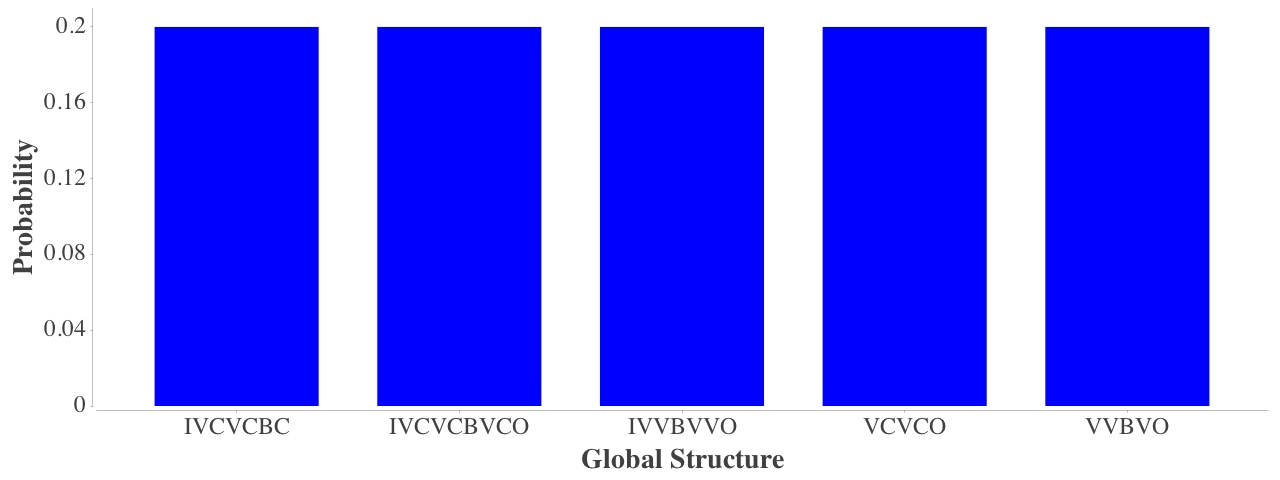
\includegraphics[width=\linewidth]{global_structure}
	\caption{\label{fig:global_structure} A visual representation of a possible probability distribution over global song structures composed of verses (V), choruses (C), intros (I), outros (O), and bridges (B).}
\end{figure}

A second approximation is a \textit{distributional model} which learns a multinomial distribution of possible structures from a corpus of composition artefacts (e.g., see Figure~\ref{fig:global_structure}). The disadvantage to the distributional model is that it can only produce structures seen in training. 

A third, more powerful approximation uses a \textit{constrained Markov model}. This model factors $P(\zeta|\nu)$ into a distribution over the number of segments in a song, $P(|\zeta|)$, and a single-order Markov model for sequences of segment types:
\[ P(\zeta|\nu) = P(|\zeta|) P(\zeta_1) \prod_{i=2}^{|\zeta|} P(\zeta_i|\zeta_{i-1}) \]
\noindent Note that an unconstrained, unsmoothed Markov model for $P(\zeta_i|\zeta_{i-1})$ provides no guarantee that a sequence of length $|\zeta|$ can or will be generated, nor that the sequence will end naturally (e.g., with an outro). With \citeauthor{pachet2011finite}'s \emph{constrained} Markov model we can constrain the length and the way the sequence ends. This modifies the way $P(\zeta|\nu)$ is factored by conditioning $\zeta_i$ on both $i$ and $\zeta_{i-1}$:
\[ P(\zeta|\nu) = P(|\zeta|) P(\zeta_1) \prod_{i=2}^{|\zeta|} P(\zeta_i|i,\zeta_{i-1}) \]
When generating, a length is sampled from $P(|\zeta|)$ and a constrained Markov model for the sampled length is constructed from the unconstrained model $P(\zeta_i|\zeta_{i-1})$ with the added constraint that the song must end on an ``end'' token. This model is capable of creating sensible structures of reasonable length that were not seen in the training data. Empirical distributions for approximating $P(|\zeta|)$ and $P(\zeta_i|\zeta_{i-1})$ are shown in Figures~\ref{fig:segment_count_per_song} and~\ref{fig:segment_transitions} respectively.

A fourth possible solution for generating global structure would be to use a generative grammar, learned or manually constructed, similar to what was done by \cite{steedman1984generative}.

\begin{figure}
	\centering
	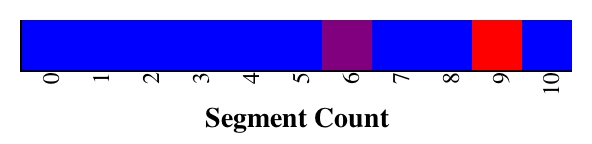
\includegraphics[width=.8\linewidth]{segment_count_per_song}
	\caption{\label{fig:segment_count_per_song} A visual representation of a possible probability distribution over the number of segments per song. Red corresponds to high probability, blue to low.}
\end{figure}

\begin{figure}
	\centering
	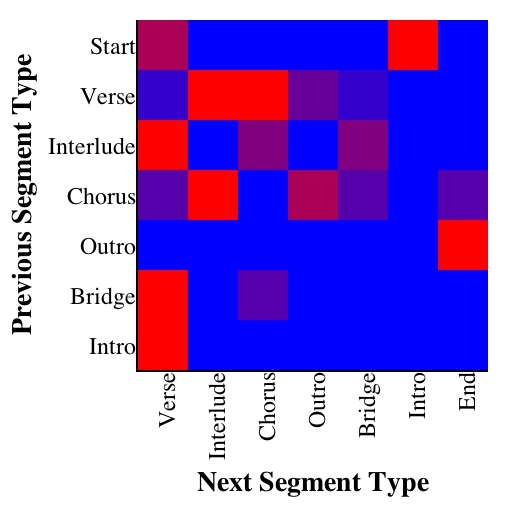
\includegraphics[width=.6\linewidth]{segment_transitions}
	\caption{\label{fig:segment_transitions} A visual representation of a possible single-order Markov transition matrix for segment types. Red corresponds to high probability, blue to low. The results largely agree with intuition. For example, songs generally start with an intro and occasionally with a verse; songs generally end with an outro and occasionally a chorus; and segments of the same type do not generally follow one another.}
\end{figure}

In addition to global structure, we also model \emph{segment structure}, $P(\sigma|\nu,\zeta)$. Though this segment structure could be included as part of global structure, modeling this substructure independently leverages principles of abstraction and polymorphism in order to facilitate novel combinations of substructures. For example in story-generation the global structure might dictate something about the abstract content of each paragraph (e.g., protagonist faces a trial, protagonist learns lesson, etc.), whereas the segment structure might define the narrative style for the paragraph (e.g., dramatic visualization, retrospection, dialogue, etc.) or add definition to the abstract content (e.g., the trial is a storm, the trial is losing a loved one, etc.). Modeling these structures independently enables the model to combine narrative styles with plot elements in ways that were not seen during training.

A segment in a composition (e.g., a verse) exhibits structure in the number of measures, the number of syllables or notes per segment, which lyrics rhyme or repeat, and patterns in harmony, pitch, or rhythm. We define a segment structure for lyrical composition as a sequence of pairs $\sigma = ((l_1,C_1),\mydots,(l_{|\zeta|},C_{|\zeta|}))$, where $l_i$ is the measure length of the $i$th segment (corresponding to $\zeta_i$) and $C_i = \{{c_{i1},\mydots,c_{in}}\}$ is a set of constraints which apply to the $i$th segment.

Constraints define restrictions on different musical viewpoints in order to create rhyme and repetitive motifs. A constraint, $c_{ij}$, is defined for a particular viewpoint $v\in\{Harmony, Pitch, Rhythm, Lyric\}$; with a condition $d\in\{Equals, Matches, RhymesWith, HasExpectation\}$; with a Boolean value $t$ that defines whether the condition $d$ needs to be satisfied or unsatisfied in order to satisfy the constraint $c_{ij}$; and with $m\in[0,l_i)$ and $b\in[0.0,bpm_m)$ representing the measure and beat offset within the segment to which the constraint applies ($bpm_m$ is the beats per measure of $m$). Each condition $d$ has different sub-variables and dimensionality:

\begin{itemize}
\item $Equals$ conditions - $c_{ij} = (v,d=Equals,t,m,b,S)$, where to satisfy $d$, the $v$ token at or near measure $m$, beat $b$ must equal a $v$ token in the set of tokens $S$ if $t$ is $true$ and must not equal any $v$ token in $S$ if $t$ is $false$.
\item $Matches$ conditions - $c_{ij} = (v,d=Matches,t,m,b,$ $m_2,b_2)$, where to satisfy $d$ the $v$ token at or near measure $m$, beat $b$ and at or near measure $m_2$, beat $b_2$ within the segment must be equal if $t$ is $true$ and not equal if $t$ is $false$.
\item $RhymesWith$ conditions - $c_{ij} = (v=Lyric,d=Rhy\-mes\-With,t,m,b,m_2,b_2)$, where to satisfy $d$ the $Lyric$ tokens at or near measure $m$, beat $b$ and at or near measure $m_2$, beat $b_2$ within the segment must rhyme if $t$ is $true$ and not rhyme if $t$ is $false$.
\item $HasExpectation$ conditions - $c_{ij} = (v,d=HasEx\-pectation,t,m,b,s)$, where to satisfy $d$ the $v$ token at or near measure $m$, beat $b$ must have an expectation value above a threshold $s$ if $t$ is $true$ and not have an expectation value above $s$ if $t$ is $false$. This constraint can be used to create a structure of expectation (as discussed by \citeauthor{meyer2008emotion} \cite{meyer2008emotion}) in order to model patterns of surprise and tension.
\end{itemize}

Note that the attribute $t$ could allow the system to learn how to intelligently break rules. For example, the system could intelligently learn when \emph{not} to rhyme when perhaps a rhyme would normally be expected.

We define the distribution over segment structures $\sigma$ as
\[ P(\sigma|\nu,\zeta) =  \prod_{i=1}^{|\zeta|} P(C_i | l_i) P(l_i|\zeta_i). \]

To approximate $P(l_i|\zeta_i)$ we can learn a probability distribution over segment lengths conditioned on segment type (see Figure~\ref{fig:measure_count_by_segment}). Under the assumption that the constraint set for a segment is independent of the segment type given its length, we can approximate $P(C_i | l_i)$ using a probability distribution over sets of constraints conditioned on segment length (e.g., see Figure~\ref{fig:segment_structure}).

\begin{figure}
	\centering
	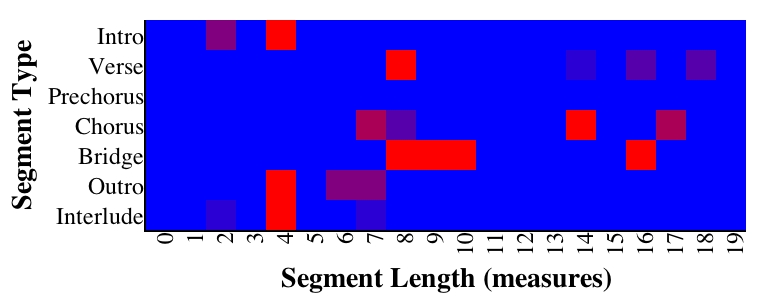
\includegraphics[width=\linewidth]{measure_count_by_segment}
	\caption{\label{fig:measure_count_by_segment} A visual representation of an empirically derived probability distribution over song segment lengths, conditioned on segment type. Red corresponds to high probability, blue to low. The results largely agree with intuition: intros, outros, and interludes tend to be shorter; verses, bridges and choruses tend to be longer.}
\end{figure}

\begin{figure}
	\centering
	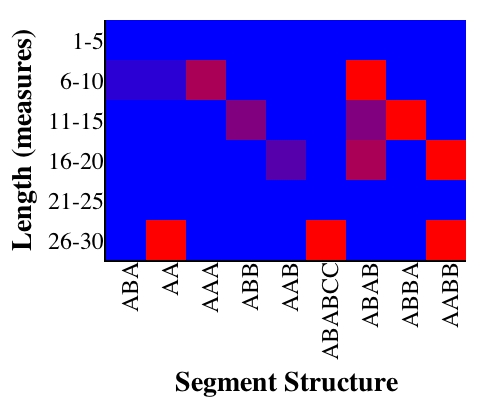
\includegraphics[width=.7\linewidth]{segment_structure}
	\caption{\label{fig:segment_structure} A visual representation of an empirically derived probability distribution over song segment rhyme structures conditioned on segment length. Red corresponds to high probability, blue to low.}
\end{figure}

Much of the work that has been done with finite-length Markov processes with constraints has required the user to specify the desired constraints in the composition process (e.g., \cite{pachet2014imitative,barbieri2012markov}). This step of learning a model of constraints gives the system increased autonomy to choose its \emph{own} constraints and then generate artefacts to meet those constraints.

With regard to modeling distributions for implicit features of an artefact (e.g., rhyme constraints), empirically-derived distributions can incur significant AI challenges. Artefacts used for training often fail to label global and even segment structure, and therefore these implicit features must be manually labeled or somehow inferred. Though our current system learns structure from a small manually-annotated dataset, our goal in future work is to use sequence alignment over multiple viewpoints to infer global structure, finding regions of a composition where harmony, melody, and lyrics all match (i.e., chorus) or where only harmony and melody match (i.e., verse). Sequence alignment is also a promising approach to finding segment structure (e.g., \citeauthor{hirjee2010using} \cite{hirjee2010using} use alignment to detect rhyme scheme).

Having modeled the abstract structural representation, the system proceeds to model the \emph{operational} representation of the artefact (e.g., paint strokes, narrative text, recipe ingredients, etc.). Whether modeled jointly or factored, the operational variables describing the artefact composition are conditioned on the constraints imposed by the intention and global/segment structure. Adapting Pachet and Roy's definition of a jazz leadsheet (\citeyear{pachet2014imitative}), we define the operational representation of a lyrical composition as parallel sequences of chords $\eta$, notes $\mu$, and lyrics $\lambda$ each with the same total duration. $\eta$, $\mu$, and $\lambda$ are defined in the following sections.

\subsubsection{Harmony, $P(\eta|\nu,\tau)$}

We define a harmony as a sequence of positioned chords $\eta = (C_1,\mydots,C_n)$ of arbitrary length. Each positioned chord $C_i = (I_i,d_i)$ has an identity $I_i = (r_i,q_i,s_i)$, with root pitch $r_i\in[0,11]$, chord quality $q_i$ (e.g., major, minor, dominant, etc.\footnote{possible values for $q_i$ are defined according to the MusicXML 2.0 specification for chord qualities}), and bass pitch $s_i\in[0,11]$; and a duration $d \in \mathbb{R}_{>0}$. We normalize all root and bass pitches based on the labeled key signature of the training instance at the harmony position.

\begin{figure}
	\centering
	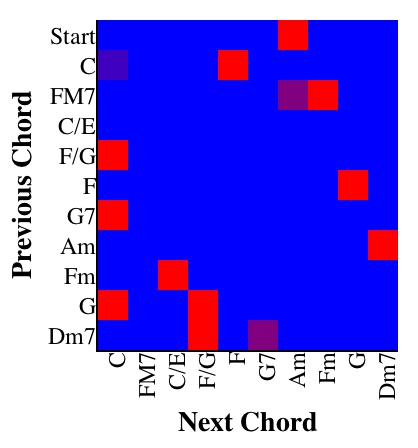
\includegraphics[width=.6\linewidth]{harmony}
	\caption{\label{fig:harmony} A subsection of a visual representation of an empirically derived single-order Markov transition matrix for harmonic chord sequences for chorus segments. Red corresponds to high probability, blue to low. As expected for songs normalized to the key of C major, there is high probability that the song starts on a C major chord. }
\end{figure}

We can factor $P(\eta|\nu,\tau)$ into independent sequential models regulating chord duration and chord identity:
\small
\[ P(\eta|\nu,\tau) = P(I_1|\tau) P(d_1|\tau) \prod_{i=2}^n P(I_i|I_{i-1},\tau) P(d_i | d_1,\mydots,d_{i-1},\tau). \]
\normalsize
\noindent  In this formulation, the length of the sequence $n$ is dynamically determined such that $\Sigma_{i=0}^n d_i$ equals the segment duration.

Deciding how to implement $P(I_i|I_{i-1},\tau)$ and $P(d_i | d_1,\mydots,d_{i-1},\tau)$ is non-trivial. A few possibilities for probabilistic sequence models include:
\begin{enumerate}
\item a \textit{fixed generator} generates a fixed token, essentially ignoring conditioned variables
\item \label{model:distribution_model}a \textit{probability distribution} over tokens, conditioned on segment type and/or beat position, but not previous token
\item a \textit{Markov model} that generates a new sequence for each segment, independent of segment type
\item \label{model:seg_model}a \textit{set of Markov models} - one model per segment type
\item a \textit{hidden Markov model} - hidden states representing the segment type
\end{enumerate}
\noindent Each model has limitations that must be considered in the context for which it is intended. Of these, our implementation uses model~\ref{model:seg_model} for $P(I_i|I_{i-1},\tau)$ (see Figure~\ref{fig:harmony}) and model~\ref{model:distribution_model} for $P(d_i | d_1,\mydots,d_{i-1},\tau)$ (for a discussion of the relative musical merits of these models see \citeauthor{bodily2017Mume} \cite{bodily2017Mume}).

The decision to assume that duration and chord are independent, though potentially erroneous, is deliberate. This is based on the reasoning that the strength of a probabilistic model depends on the number of instances used to train the model. Each time a distribution adds a conditional variable, the power of the model is reduced. We feel that the duration and chord are sufficiently independent that the model strength recovered by assuming independence outweighs the cost of ignoring any dependence between them.

\subsubsection{Melody, $P(\mu|\nu,\tau,\eta)$}

A melody is a sequence of positioned notes $\mu=(N_1,\mydots,N_n)$ of arbitrary length. Each note $N_i = (p_i,d_i)$ has a pitch $p_i\in[-1,127]$  (corresponding to a MIDI note value, -1 representing a rest) and a duration $d_i \in \mathbb{R}_{>0}$. We factor $P(\mu|\nu,\tau,\eta)$ into independent sequential models regulating note pitch and duration:
\small
\[ P(\mu|\nu,\tau,\eta) = P(p_1|\eta) P(d_1|\tau) \prod_{i=2}^n P(p_i|p_{i-1},\eta) P(d_i|d_{i-1},\tau). \]
\normalsize
\noindent The length of the sequence $n$ is dynamically determined such that $\Sigma_{i=0}^n d_i$ does not exceed the segment duration.

Of these models only pitch is conditioned on $\eta$. To model $P(p_i|p_{i-1},\eta)$ our implementation uses a single-order Markov chain of scale steps where the scale is defined by the contextual harmony of $\eta$. To model $P(d_i|d_{i-1},\tau)$ we use a segment-specific Markov chain of note durations (see Figure~\ref{fig:melody_rhythm}). Any of the probabilistic sequence models considered for harmony could also be considered here.

\begin{figure}
	\centering
	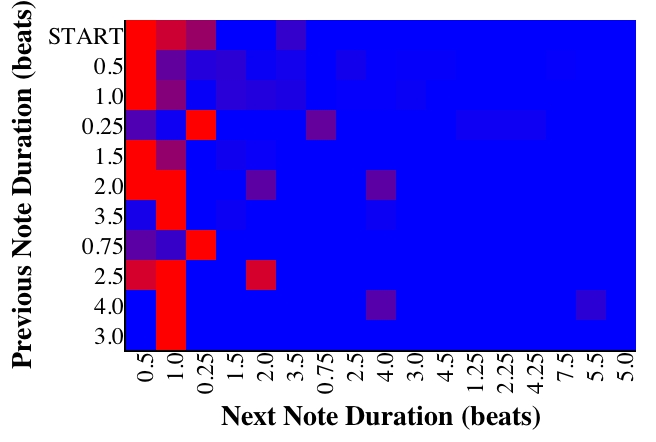
\includegraphics[width=\linewidth]{melody_rhythm}
	\caption{\label{fig:melody_rhythm} A visual representation of an empirically derived single-order Markov model for melodic rhythm durations for verse segments in 4/4. Red corresponds to high probability, blue to low.}
\end{figure}

\subsubsection{Lyrics, $P(\lambda|\nu,\tau,\mu)$}

Several models of natural language generation (NLG) and in particular NLG in poetry and music have been published \cite{paris2013natural}. As these models continue to improve, so will their application in lyrical composition. This demonstrates the robustness of the HBPL framework: as improved submodels are conceived and implemented, the joint model is also improved.

We define lyrics as a sequence of stressed syllables $\lambda=(S_1,\mydots,S_n)$ where $|\lambda| \le |\mu|$. A stressed syllable $S_i = (t_i, p_i, \epsilon_i)$ has a text representation $t_i$, a pronunciation $p_i$ (e.g., sequence of ARPAbet phonemes), and a stress $\epsilon_i\in[0,2]$. Each syllable $S_i\in\lambda$ corresponds to one and only one note $N_j\in\mu$.
\begin{figure*}
	\centering
	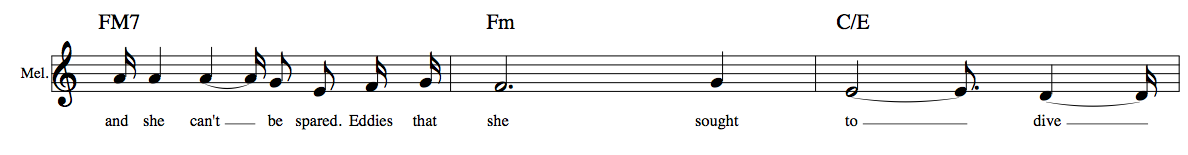
\includegraphics[width=\linewidth]{example}
	\caption{\label{fig:example_composition} Three measures of a sample composition generated using the HBPL framework. The full composition and others can be found online at \url{popstar.cs.byu.edu}.}
\end{figure*}

We factor $P(\lambda|\nu,\tau,\mu)$ to construct $\lambda$ as a sequence of lyric phrases $(\phi_1,\mydots,\phi_n)$ where the number of phrases $n$ and the length $l_{\phi_i}$ (in syllables) of each phrase are computed as a function of the notes in $\mu$ and the rhyme constraints in $\tau$ (i.e., we assume rhyme constraints denote phrase endings):
\[ P(\lambda|\nu,\tau,\mu) = \prod_{i=1}^n P(\phi_i | l_{\phi_i},\nu,\tau) P(l_{\phi_i} | \mu,\tau). \]
We empirically derive $P(l_{\phi_i} | \mu,\tau)$. For $P(\phi_i | l_{\phi_i},\nu,\tau)$ we create a probability distribution of lyric templates conditioned on $l_{\phi_i}$ which we use to sample templates. These templates, the $RhymesWith$ constraints of $\tau$, and $\nu$ are given as input to an independent module that generates novel, intentioned lyrics (see \citeauthor{bay2017ICCC} \cite{bay2017ICCC}). The module uses existing lyric segments as syntactic templates for the creation of novel lyric segments. It intelligently selects and replaces words based on 1) semantic similarity, 2) part-of-speech tag, 3) the cultural and thematic intention of $\nu$, and 4) the rhyme constraints imposed by $\tau$.

The advantage of using a template-based approach to lyrics generation is that it maintains syntactic coherence. The primary shortcomings are that resulting lyrics provide limited syntactic novelty from the training data and make no inherent effort at providing global semantic cohesion.

\subsubsection{A Note on Constrained Markov Models}

\citeauthor{pachet2011finite}'s constrained Markov model requires that the length of the sequence be defined \emph{a priori} \cite{pachet2011finite}. One short-coming in our current implementation is that because we have included duration as part of the definition for both harmony and melody (rather than having each chord or note representative of a fixed duration as demonstrated by \citeauthor{pachet2014imitative} \cite{pachet2014imitative}) the length of a harmony or melody sequence depends on the durations of each sampled chord or note. While this violates the Markov property and prevents us from being able to effectively use constrained Markov models, we favor the current implementation for reasons related to data sparsity issues and the complexity of implementing higher-order constrained (hidden) Markov model. We hope in the future to overcome both of these hurdles and to shift to ``Markov-friendly'' definitions for melody and harmony in order to more fully incorporate the constraints defined in $\tau$ using constrained Markov or constrained hidden Markov models.

\section{Results and Discussion}

We present results of implementing the HBPL framework in the context of a discussion of some of the model's implications. We trained submodels on a small manually-annotated subset of the Wikifonia leadsheet dataset.

\subsection{Using the Joint as a Submodel}

Because of the hierarchical nature of HBPL, a joint model of an artefact class (e.g., the model of $P(\gamma|\iota)$ just described) can serve as a submodel for other models. For example, we define the joint probability distribution on inspirations $\iota$, compositions $\gamma$, and renderings $\rho^{m}$ as follows,
\[ P(\iota,\gamma,\rho^1, ..., \rho^m) = P(\iota)P(\gamma|\iota) \prod_{m=1}^M P(\rho^m|\iota,\gamma). \]
In essence we decompose a model of music \emph{creation} to individually model the inspiration for the artefact, the symbolic (abstract) representation of the artefact, and the concrete rendering of the artefact. 

\subsubsection{Inspiration, $P(\iota)$}

\emph{Inspiration} (i.e., the method for deriving intention) may be more closely related to an artist's or system's ``creative spark''. For example, observers often perceive greater creativity in artefacts which in some way relate to them or to their culture \cite{colton2008creativity}. In the joint probability distribution on inspirations $\iota$, compositions $\gamma$, and renderings $\rho^{m}$, we define $P(\iota)$ not as the distribution over intentions, but as the distribution over inspiring sources for the intention. In other words, not ``what was the artefact intended to communicate?'', but ``what was the inspiring \emph{source} for what the artefact intended to communicate?''

In general this demonstrates an unanticipated benefit of factorization: we can condition on any variable that could be argued to influence the artefact's creation. Many creative systems implicitly define inspiration based on the corpora that the data trains on. With the concept learning framework, we can model this attribute explicitly.

This represents an aspect not present in the model originally presented by Lake et al. \cite{lake2015human}: not only are we modeling \textit{what} artefacts can be generated, but also \textit{why} they are generated. One possible way to model inspiration is to use an observer's environment or culture as an inspiring source. Research in electroencephalogram-based affective computing (i.e., reading brain waves) suggests that computers may soon be able to perceive an observer's emotional state beyond those of their human counterparts \cite{volioti2016mapping}. Alternatively, inspiration could be modeled using sentiment analysis in a variety of online domains. We plan to explore models of inspiration further in future research.

\subsubsection{Rendering, $P(\rho^{m}|\iota,\gamma)$}

The example model $P(\gamma|\iota)$ described above defines symbolic lyrical compositions (i.e., a leadsheet). However, evaluating an abstract artefact generally requires a concrete rendering of the artefact, whose distribution we model as $P(\rho^{m}|\iota,\gamma)$. As a proof of concept, we implemented and trained the described HBPL model on a small corpus of hand-annotated lyrical pop composition data. To concretely render compositions created using this model, we generated both printed sheet music (e.g., Figure~\ref{fig:example_composition}) and an MP3 audio recording\footnote{audio recordings can be found at \url{popstar.cs.byu.edu}}. Our MP3 audio file features computer-sung lyrics accompanied by synthesized piano and bass comping chords\footnote{generated using Harmony Assistant (v9.7.0f) and Virtual Singer (v3.2)}.

\subsubsection{Implications for Recommendation Systems}

Lake et al. present the model of $P(\psi)$ given in equation \ref{eq:1} as a submodel of the factoring of the joint probability distribution on character types $\psi$, tokens $\omega^m$, and binary images $I^m$ \cite{lake2015human}:
\small
\[ P(\psi, \theta^1, \mydots,\theta^M,I^1,\mydots,I^M) = P(\psi) \prod_{m=1}^{M} P(I^m|\theta^m)P(\theta^m|\psi). \]
\normalsize
This means that given an image, the system can discover the motor program (i.e., abstract character type) that most likely generated it. This allows the system to one-shot classify and generate pairs of images that represent the same character type (specific examples of which were not seen in training). 

By analogy, a model for $P(\gamma)$ (similar to $P(\gamma|\iota)$ just described) could be inserted into a joint probability on composition types $\gamma$, arrangements $\alpha^m$, and audio recordings $\rho^m$,
\small
\[ P(\gamma,\alpha^1,\mydots,\alpha^M,\rho^1,\mydots, \rho^M) = P(\gamma) \prod_{m=1}^M P(\rho^m|\alpha^m)P(\alpha^m|\gamma). \]
\normalsize
The implications of this model are more broadly significant: the HBPL framework is capable of inferring abstract representations of concrete artefacts, representations which more directly define meaning, composition, and causality. This is significant for two reasons. First, in some realms of creativity, simply deriving the abstract representation of an artefact is valuable (e.g., automatically transcribing sheet music from audio). Second, having an abstract representation allows concrete artefacts to be compared according to symbolic, conceptual criteria (e.g., recommendation systems based on meaning, or in the case of music, harmony, melodic pitch or rhythm, etc.). Though work has been done to approximate $P(\alpha^m|\gamma)$ \cite{benetos2013automatic}, effective comparison of artefacts hinges on the other terms in the factorization, $P(\gamma)$ and $P(\rho^m|\alpha^m)$, which are lacking.

\subsection{Fitness and Self-Evaluation}

The HBPL framework is designed to restrict the generation process \emph{in situ} to produce only meaningful artefacts (as compared to a generate-and-test procedure). As discussed by \citeauthor{Ventura2016} \cite{Ventura2016}, this ``baked-in'' self-evaluation mechanism has the added benefit of being able to explain to some extent both the novelty, value, and motivation behind generated artefacts. Given its ability to compute probabilities, the HBPL framework could thus also be potentially leveraged as a fitness function for other types of generative models.

\subsection{Big (Need for) Data}

Any empirically-driven model requires training on a dataset representative of the artefact domain. Even if we had digital access to all of the compositions ever written, it would represent an infinitesimal portion of the songs that \emph{could} be written. This is a challenge in many machine learning domains. Unique to the pop music domain, however, is that data is highly proprietary. What \textit{is} available is extremely limited and of relatively poor quality. Compared to natural language, artefacts in music generally require relatively complex representations and relatively few possess the domain knowledge required to generate or transcribe the needed data. Among those who \textit{do} understand and use it, music formatting can vary wildly and inexactly---creating additional challenges for a by-the-bit computer parser. Computers will only learn to speak music as quickly as we either formalize and ubiquitize the language of music \textit{or} endow computers with AI tools to fill in the gaps on their own.

The particular challenge of accessing high-quality symbolic \emph{pop} music datasets is significant. There is a dearth of well-annotated resources for those interested in studying any or all of the aspects of pop music composition. There is, however, much we can do to improve the situation. First, we need to make resources that \textit{are} available more accessible (guitar tabs, lyrics sites, beatles). Second, we need to establish a better case for how society and industries stand to benefit from computational pop music research in order to generate a productive dialogue for the support and collaboration of those in possession of large pop music datasets (sheet music sites, spotify, etc., asking for APIs, etc). Note that this is different than asking them to simply give us their proprietary data. Third, we can do more to recognize contributions of novel datasets.

\section{Conclusion}

HBPL is a powerful framework for accomplishing tasks in computational creativity. Using principles of compositionality, causality, and learning-to-learn, such models are able to effectively learn and generate examples of complex creative concepts. Its probabilistic framework lends itself well to modeling important aspects of creativity such as inspiration and intention. The HBPL framework by nature compels researchers in domain-specific subareas of computational creativity to engage in the debates that the artists themselves are having, namely ``how should an artefact be created?'' and ``does it matter?'' To the extent that these challenges are effectively addressed on the scale of defining and training subconcept models, the HBPL model represents a useful framework for designing and assessing creative systems.

\chapter{Floating and Dynamic Constraints in Non-Homogeneous Markov Models}

\emph{We plan to submit this paper to the 2018 Association for the Advancement of Artificial Intelligence Conference on Artificial Intelligence}

\section{Introduction}

In many sequential domains structure and meaning are created as the result of constrained relationships between elements at disparate sequence positions. In proteomics bonds between amino acids at distinct positions are essential for protein folding. In natural language semantic cohesion is achieved by part of speech agreements. Musical motifs and patterns of repetition are observed to increase the ease with which information is processed by the brain \cite{Nunes2014}. Probabilistically modeling structured sequences is problematic for stochastic processes including Markov models, which are commonly used for classification and generation in these domains. 

Constrained or \textit{non-homogeneous Markov models} (NHMMs) \cite{pachet2011finite} have been more recently presented as a way of introducing more control, essentially representing sequence modeling as a constraint satisfaction problem (CSP). By constraining against sequences that are uncharacteristic of a a particular domain, NHMMs are able to generate and classify sequences more efficiently and effectively. 

For the most part NHMMs have been presented that are based on 1-order Markov models \cite{barbieri2012markov,roy2013enforcing,papadopoulos2015exact}. In this form NHMMs exhibit significant limitations. First, because NHMMs require the definition of constraints applied at specific positions, there is no leniency to allow a particular constraint to be allowed across a range of positions. Such an ability would be helpful, for example, for constraining semantic meaning in natural language phrases without having to be picky about where it occurs. Second, because NHMMs operate solely using static unary constraints, many types of relational constraints cannot be effectively modeled. Dynamically-defined relationship variables would be effective, for example, in imposing bonds between biological molecules, in forming rhymes, and in creating grammatic cohesion or semantic relationships between words. Though some general comments have been made with respect to implementing higher-order models (e.g., \cite{pachet2011finite}), several significant advantages of NHMMs---including those required to overcome the above-mentioned shortcomings---have been overlooked and emerge only when considered in their higher-order implementations.

In this paper we demonstrate two new classes of constraints, \textit{floating constraints} and \textit{dynamic constraints}, which aim to overcome the limitations of fixed-position and static constraints in NHMMs. We effectuate these constraints using $d$-order NHMMs (i.e., a NHMM built from a $d$-order Markov model). Sampling sequences with dynamic and floating constraints is theoretically possible using regular constraints in single-order models \cite{pesant2004regular,papadopoulos2014avoiding,papadopoulos2015exact,bodily2018relational}. However, whereas the computation time of NHMMs have been shown to grow linearly in the length of the sequence to be generated, the same has not yet been shown in the regular constraint model \cite{bodily2018relational}. Furthermore, even with the use of regular constraint, the approach demonstrated here is mandatory for any application of dynamic or floating constraints within the Markov window.

We demonstrate three examples that utilize dynamic and floating constraints in NHMMs: a lyric generation model with dynamic rhyming constraints and floating part-of-speech (POS) constraints; a haiku generation model with floating semantic constraints; and a prosodic rhythm generation model with floating stress and time signature constraints. In the case of the lyric generation model, we include an empirical assessment of five higher-order NHMMs with floating and dynamic constraints.

\section{Methods}

A finite-length NHMM $\tilde{M}$ is created given a finite length $l$, a trained Markov model $M$, and a set of positioned constraints $C$. $\tilde{M}$ has the following properties:
\begin{enumerate}
\item $\tilde{M}$ only assigns probability to sequences that satisfy $C$;
\item Sequences that satisfy $C$ are assigned the same probability in $M$ and $\tilde{M}$ up to a constant factor.
\end{enumerate}
$\tilde{M}$ is derived from $M$ by replicating the transition matrix of $M$ for each of $l-1$ positions and then imposing the constraints in $C$ to modify the matrices at specific positions. The CSP is made arc-consistent, meaning states are iteratively removed at neighboring positions to ensure that all constraints are satisfied via any remaining solution. Probabilities are then normalized to ensure remaining solutions are assigned the same relative proportion of the probability density \cite{pachet2011finite}.

The properties and construction of $\tilde{M}$  hold true regardless of the order of $M$. $M$ has traditionally been presented as a single-order Markov model $M_1$ which generates a sequence according to the probability function $P(X_1,\cdots,X_n) = P(X_1)\cdot P(X_2|X_1)\cdots P(X_n|X_{n-1})$. However, $M$ may just as easily be a $d$-order Markov model, $M_d$, which generates a sequence with a longer memory such that $P(X_i|X_1,\cdots,X_{i-1}) = P(X_i|X_{i-d},\cdots,X_{i-1})$. The fact that the order of $M$ does not affect the NHMM construction falls out immediately from the observation that $M_d$ can by created using a single-order Markov model on an alphabet of $d$-grams \cite{papadopoulos2015exact}. More precisely this means changing the finite state space ${A_1} = \{a_1, \cdots,a_n\}$ for $M_1$ (where each element $a_i \in A_1$ is a raw token) to a state space $A_d = \{P_1,\cdots,P_m\}$ where each element $P_j \in {A_d}$ represents a $d$-length sequence of tokens $P_j = (s_1, \cdots, s_d)$ (where $s_i \in {A_1}$). Thus a transition $j\Rightarrow k$ in ${M_d}$ represents a transition from sequence $P_j$ to sequence $P_k$ where $s_2, \cdots, s_d$ in $P_j$ and $s_1, \cdots, s_{d-1}$ in $P_k$ are identical subsequences. 

We thus implement a $d$-order NHMM, $\tilde{M_d}$, following the same construction presented by \citeauthor{pachet2011finite} (\citeyear{pachet2011finite}) for building a single-order NHMM $\tilde{M_1}$ with the exception that we construct from $M_d$ rather than $M_1$. This modification requires no additional modification to the procedure for normalizing probabilities. 

Note that in sampling an \textit{element sequence} $(X_1,\cdots,X_n)$ from either $M_d$ or $\tilde{M_d}$, all tokens $s_1, \cdots, s_d$ in $X_1$ and the final token $s_d$ in each $X_i$ for $i>1$ are concatenated to form the generated \textit{token sequence} (e.g., see Figures~\ref{fig:higher_order_markov} and~\ref{fig:higher_order_nhmm}). Thus a $d$-order NHMM of length $l$ generates sequences of length $(d+l-1)$.

\begin{figure} 
\centering
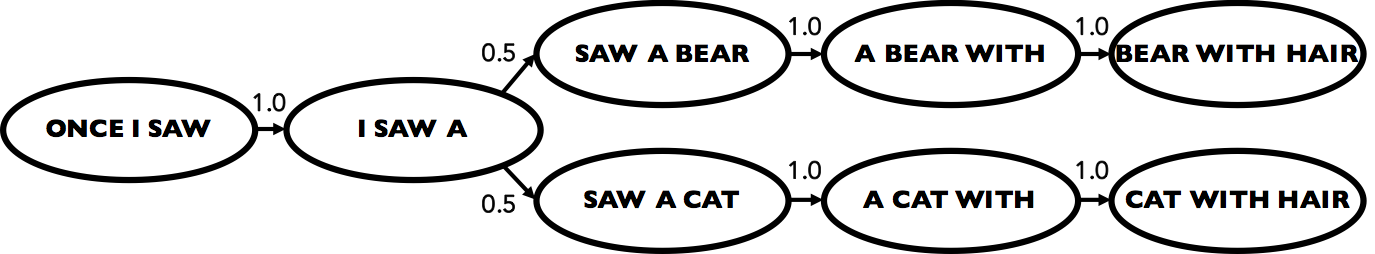
\includegraphics[width=\linewidth]{higher_order_mm}
\caption{\textit{A 3rd-Order word-level Markov model.} The model has been trained on the phrases ``once I saw a bear with hair'' and ``once I saw a cat with hair''. Since each word is a single syllable, this example also represents a syllable-level model. Each element in this model is a 3-length sequence of tokens and transitions are between sequences that overlap by all but one token. Note that though an element sequence from this model will have length 5, the generated token sequence will have length 7 (i.e., element sequence length + order - 1).}
\label{fig:higher_order_markov}
\end{figure}

\begin{figure*}
\centering
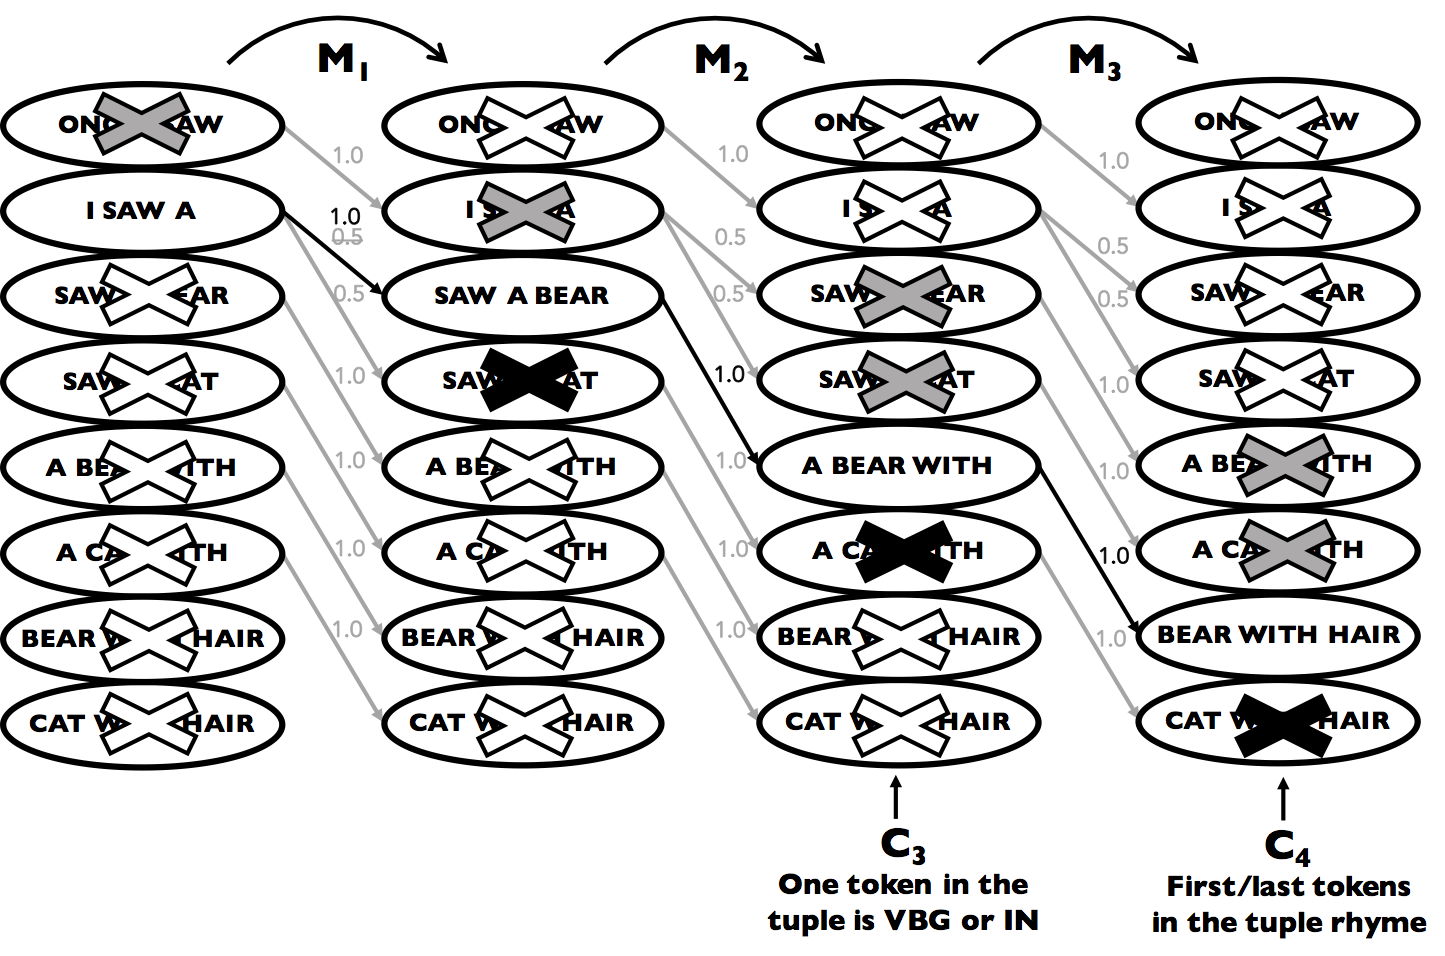
\includegraphics[width=.8\linewidth]{higher_order_nhm}
\caption{\textit{A 3rd-order NHMM of length 4.} This model is built from the Markov model in Figure~\ref{fig:higher_order_markov} and generates sequences of length 6. States marked with a white `X' are pruned due to the length constraint (i.e., transitions through these states do not result in element sequences of length 4). States marked with a gray `X' are pruned due to the addition of the $C_3$ POS constraint. This constraint is an example of a floating constraint in that the POS constraint is effectively satisfied by any satisfying token appearing at sequence positions 3, 4, or 5. States marked with a black `X' are pruned due to the further addition of the $C_4$ rhyme constraint. The $C_4$ constraint is an example of a dynamic constraint in that the token constraint at sequence position 6 effectively depends on the token at sequence position~4. Grey transitions represent transition probabilities that are zeroed as a result of applied constraints.}
\label{fig:higher_order_nhmm}
\end{figure*}

\subsubsection{Optimizing NHMM Construction}

For $n$ distinct tokens (e.g., in $A_1$), the number of potential distinct elements in $\tilde{M_d}$ is $|A_d| = n^d$, and the number of possible transitions (copied $l-1$ times) is thus $(l-1)n^{2d}$. Therefore increasing $d$ substantially increases both the time and memory required to implement $\tilde{M_d}$. We present two important optimizations for implementing $M_d$ which improve on the algorithm presented by \citeauthor{pachet2011finite} (\citeyear{pachet2011finite}). Given the sparsity of these matrices, we assume that matrices are implemented as a map that includes only non-zero transition probabilities.

First, whereas \citeauthor{pachet2011finite}'s algorithm suggests initializing \textit{a priori} new matrices $Z^{(i)} = M_d$ (i.e., the transitions of $M_d$) for $i \in [1,\cdots,l-1]$, it is far more efficient to initialize these matrices one at a time, starting from empty and only adding non-zero transition probabilities $j \Rightarrow k$ to $Z^{(i)}$ for which $j$ is reachable given $Z^{(i-1)}$. For example, if there is only one reachable state, $P_j$, given $Z^0$ (i.e., the prior probabilities of $M$), then $Z^{(1)}$ need only add transitions in $M_d$ from $P_j$ rather than copying all of $M_d$ ($L-2$ times over) and then pruning all transitions except those from $P_j$. 

Second, the addition of transitions $j \Rightarrow k$ to $Z^{(i)}$ at each position $i$ should be further limited according to whether $k$ satisfies all unary constraints and whether $j \Rightarrow k$ satisfies all transitional constraints relevant to position $i$. 

Normalization proceeds as described by \citeauthor{pachet2011finite}. In solving the DBTB problem, where viable paths are significantly reduced from applying constraints at even the first few positions, we observed improvements in speed and memory of roughly 50x as a result of these optimizations.

\subsubsection{Floating Constraints}

Higher-order NHMMs enable a class of constraints which we call \textit{floating constraints}. In essence this type of constraint allows unary (or other) constraints to be satisfied at any one of several positions rather than at a specific position. For example, rather than constrain the $i$th position of a phrase to be a particular POS, we can constrain the model such that any token in the range of positions $[i-d,i]$ must be a particular POS or such that the sequence of tokens in the range of positions $[i-d,i]$ must represent a particular meta-level POS, such as a noun phrase. Floating constraints are useful for allowing the model to have more flexibility in generation.

Floating constraints are made possible in higher-order NHMMs because a transition $j \Rightarrow k$ representing the transition from $P_j$ to $P_k$ is sufficient to determine whether the $(d+1)$-length sequence represented by the overlap of $P_j$ and $P_k$ satisfies the floating constraint (e.g., contains the requisite POS tokens)(see Figure~\ref{fig:higher_order_nhmm}).

An example of the application of floating constraints is in defining semantic constraints. \citeauthor{barbieri2012markov}~(\citeyear{barbieri2012markov}) define unary semantic constraints at fixed positions to achieve significant improvements in generating semantically related poetry. By their own admission, this approach has limited flexibility because of having to define unary constraints at specific positions. Their idea of \textit{cardinality constraints} (envisaged as future work) is itself an example of a floating constraint.

Floating constraints can also be used to not over-restricting syllable-level NHMMs when imposing word-level POS constraints. Using a word-level Markov process \citeauthor{barbieri2012markov} (\citeyear{barbieri2012markov}) are able to constrain according to \textit{word-level POS templates}. For example, the word-level POS template for the phrase ``Yesterday, all my troubles seemed so far away'' is denoted as [NN, IN, DT, NN, PRP, MD, VB, NN]. Although we can impose the same constraints using a \textit{syllable-level POS template} (e.g., [NN, NN, NN, IN, DT, NN, NN, PRP, MD, VB, NN, NN]), note that doing so reduces the expressiveness of our syllable-level model by up to a factor of $2^{l-1}$ insofar as we limit the model's ability to determine the numbers of syllables per word and words per phrase. One solution is to place POS constraints at only a subset of positions (e.g., [NN, , , IN, DT, NN, ,PRP, MD, VB, , NN]), allowing the model to fill in the gaps. This solution, however, still severely restricts the model's expressiveness. It also requires statically defining a sequence of POS tags allowed at each position, essentially limiting the number of allowable POS sequences to one.

Floating constraints provide a means of imposing word-level POS templates without sacrificing expressiveness \textit{and} with the ability to allow multiple valid POS sequences. In a syllable-level $d$-order NHMM, the $(d + 1)$-length syllable sequence deriving from each transition $j \Rightarrow k$ (e.g., ``llama wearing polka-dot pajamas'') also represents a $(d+1)$-length syllable-level POS sequence (e.g., {[NN,NN,VBG,VBG,NN,NN,NN,NNS,NNS,NNS]}\footnote{\label{note1}POS tags are those inferred by Stanford CoreNLP Toolkit \cite{Manning2014}}). A syllable-level NHMM can impose a floating word-level POS template constraint (e.g., ``must match {[NN,VBG,NN(S)]}'') over positions $[i-d,i]$ to only allow transitions $j \Rightarrow k$ whose associated $(d+1)$-length syllable-level POS sequence matches the word-level POS template of the constraint. In this way word-level POS constraints can be imposed without specifying a precise position where they must be satisfied. Furthermore, multiple POS templates can be included in the constraint to allow sequences to be validated by one of many alternatives (see Figure~\ref{fig:syntax_tree}). In this way sequences can be validated using many different word-level lexical analyses (e.g., noun phrase classifiers).

\subsubsection{Dynamic Constraints}

Higher-order NHMMs also enable what we call \textit{dynamic constraints}. A dynamic constraint allows a constraint's definition to be determined at runtime as a function of elements at neighboring positions rather than it being statically and independently defined \textit{a priori}.

For example, \citeauthor{barbieri2012markov} (\citeyear{barbieri2012markov}) demonstrate the use of NHMMs to generate lyrics for a song such that the last word in the first line is constrained to \textit{be} a particular word (``today'') and the last word in the second line is statically constrained to \textit{rhyme} with that same word. Using a dynamic constraint, the system is able to dynamically determine whether a particular pair of words rhyme without needing to know the rhyme group of either word ahead of time.

A dynamic constraint is accomplished in higher-order NHMMs by considering whether or not the $d + 1$ length sequence deriving from the transition $j \Rightarrow k$ represents a subsequence of tokens where the tokens at the two dynamically constrained positions satisfy the desired property (e.g., rhyme). This requires that the dynamically constrained positions must be within $d+1$ positions of each other, thereby maintaining the Markov property (see Figure~\ref{fig:higher_order_nhmm}). Effecting more distant rhymes requires high values for $d$ and results in less stochasticity in generated sequences. This makes dynamic constraints particularly well-suited for genres like rap where rhymes are often closely situated.

\subsubsection{Limitations of Dynamic Constraints}

In many applications the dynamic constraints of interest relate elements at very distant positions. Such dynamic constraints are not well-suited for the approach we have outlined here. As $d$ increases fewer satisfying solutions can be generated and solutions tend towards replicating exact phrases from the training corpus. \cite{papadopoulos2014avoiding} demonstrate a regular constraint solution to the problem of sampling exact phrases above a certain length from training data. Regular constraints are also a viable alternative to increasing $d$ solely for the purpose of effecting dynamic constraints \cite{bodily2018relational}.

The examples shown below use values of $d$ in the range $4 <= d <= 8$. In these cases we have elected to retain potentially exact phrases both for the sake of demonstration and because we deem that there remains an important aesthetic value in repurposing existing artefacts in novel problem domains (e.g., an \textit{objet trouv\'{e}}). In fields such as computational creativity these solutions represent a significant contribution in their own right \cite{ColtonExperimentsBrowsing}.

\section{Dynamic and Floating Constraint Examples}

In each of the three following examples we demonstrate a unique advantage afforded by dynamic and/or floating constraints in NHMMs. 

\subsection{Dynamic Relational Constraints in Lyrics}

We demonstrate the use of dynamic constraints in the context of a lyric-generation problem which we call the \textit{Down by the Bay (DBTB) problem}. ``Down by the Bay'' is a traditional song requiring improvisation of novel lyrics which conform with rhythmic, rhyming, and part-of-speech (POS) patterns representative of the song's characteristic structure. Incidentally this task has been the focus of many studies in behavioral sciences and education \cite{jalongo1997using,pasiali2004use,robb2008randomized,towell1999motivating,kolb1996read}.

After careful consideration of several prototypical solutions to the DBTB problem, we define a set of constraints for solving the DBTB problem with a sequence of length $l$ as follows:

\begin{enumerate}
\item The word at position 1 must be `a' or `an'\footnote{1-based numbering is used throughout the paper}.
\item The $l$th syllable must be the last syllable in a word.
\item The rhythmic template for $p$ must be one of the following: [011001], [0110101], [01010010], [01101011], or [01010101010].
\item \label{mandatory_rhyme_constraint}The first and last stressed syllables must rhyme.
\item \label{optional_rhyme_constraint}If the rhythmic template for $p$ ends with $0$, then the second and last \textit{un}stressed syllables must also rhyme.
\item \label{POS_floating_constraint}The syntax of the phrase must be that of a noun phrase.
\end{enumerate}

Because there are variable satisfactory lengths for $p$ and the length $l$ for a NHMM must be fixed \textit{a priori}, we create a syllable-level NHMM for each rhythmic template, adjusting constraint sets for each according to the corresponding template. %For example, from the solution ``a bear combing his hair'' which aligns to beats 0, 1, 5, 6, 8, and 9, we define a rhythmic template of [011001] together with the corresponding POS and token constraints relevant to these positions. %We discuss the challenge of automating the generation of rhythmic templates in Section~\ref{automatic_rhythmic_template_generation}.

Note that constraints \ref{mandatory_rhyme_constraint} and \ref{optional_rhyme_constraint} are easily implemented using dynamic constraints and constraint \ref{POS_floating_constraint} is easily implemented using a floating constraint. The rest are also easily implemented using fixed-position unary constraints.

%\subsubsection{A Syllable-Level Markov Model}
%
%There are several advantages to using a syllable-level as opposed to a word-level Markov model. First, for much of poetry and song lyric generation we think about music and poetry at a syllable-level, not at a word level. Many poetic forms (e.g., haiku, limericks, etc.) dictate the number (and sometimes stress pattern) of syllables that should appear in each line. Though song lyrics do not directly impose syllabic requirements, melodic rhythm and rhyme constraints place some limitations on the number and stress patterns of syllables. 
%
%Second, a syllable-level Markov model has greater expressive power than a word-level model. Although \citeauthor{barbieri2012markov} (\citeyear{barbieri2012markov}) are able to constrain the number and stress patterns of syllables in a line in their \textit{word-level} Markov model using word-level rhythmic templates, this approach has significant limitations. For example, the word-level rhythmic template for the phrase ``Yesterday, all my troubles seemed so far away'' is denoted as [100, 1, 1, 10, 1, 1, 1, 01]. Consider that a word-level Markov model constrained to match this rhythmic template would be capable of generating only the first of the following phrases:
%
%\begin{itemize}
%\item ``innocence of a story I could leave today'' ([100, 1, 1, 10, 1, 1, 1, 01])
%\item ``innocence I imagined I could leave today'' ([100, 1, 110, 1, 1, 1, 01])
%\item ``innocence of a story in an alleyway'' ([100, 1, 1, 10, 1, 1, 101])
%\end{itemize}
%
%\noindent Although the word-level rhythmic template and Markov model would only be capable of expressing the first, all three of these phrases have the same \textit{syllable}-level rhythmic template (i.e., [100111011101]), making them reasonable solutions to the problem we really care about solving. In fact, for a phrase with 12 syllables (as in our example), there are $2^{11}$ possible word-level rhythmic templates for the equivalent syllable-level rhythmic template. Using a word-level rhythmic template (and therefore word-level Markov model) in this instance would reduce the expressive power by $2^{11}$ times. Thus beyond being more conceptually accurate, a syllable-level model is simply more expressive than a word-level model. 
%
%Third, a syllable-level Markov model gains advantages in being able to impose constraints at the syllable-level rather than at the word-level. As an example, consider that one phrase has been constrained to end with the word ``repose'' and that the following phrase should be statically constrained to end with \textit{two} syllables that rhyme with ``repose''. For a syllable-level model, this is straightforward: place the appropriate syllable-level rhyme constraint on each of the last two positions in the verse. For a word-level model, this is not straightforward: phrases ending with a monosyllabic word (e.g., ``he goes'') would require \textit{two} rhyme constraints whereas those ending with a multisyllabic word (e.g., ``egos'') would require only a \textit{single} rhyme constraint. Thus the word-level model requires constraining the number of syllables in the last word in order to be able to implement bisyllabic rhyme constraints. The ambiguity of where to place constraints is further compounded in dynamic multisyllabic rhyme constraints (as in the DBTB problem).
%
%\subsubsection{Defining Syllable Tokens}
%
%Careful decisions have to be made about what constitutes a token in a Markov model. For example, if the derivative word is not included in defining a syllable token, it is possible to generate sequences of syllables that are not real words (see Figure~\ref{fig:syl_models}). Including the derivative word as part of a syllable token definition also ensures that the word-to-word probabilities contained in the (single-order) word-level Markov transition matrix are preserved in the syllable-level model. The syllable's position within the derivative word must be included to protect against cases where the word has multiple instances of a given syllable. The token must also (directly or indirectly) possess information needed to apply constraints including constraints which ensure that phrases start with the first syllable in a word and end with the last syllable in a word. In our syllable-level NHMMs we define a syllable token essentially as a function of its derivative word and the syllable position within the derivative word. From these can be inferred the syllable's constituent phonemes, stress, POS, semantic meaning, and role as starting or ending syllable.
%
%\begin{figure}
%    \centering
%    \begin{subfigure}[b]{.7\linewidth}
%        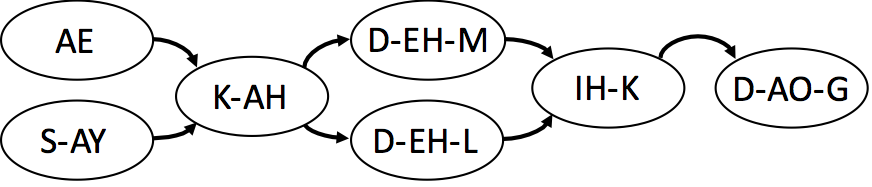
\includegraphics[width=\linewidth]{syl_model_1}
%        \caption{A Word-Independent Syllable-Model}
%        \label{fig:word-independent}
%    \end{subfigure} 
%    \begin{subfigure}[b]{.7\linewidth}
%    	\vspace{.3cm}
%        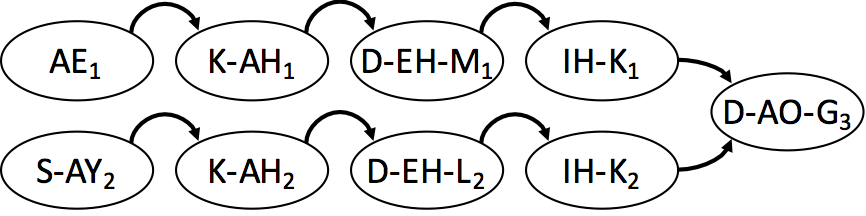
\includegraphics[width=\linewidth]{syl_model_2}
%        \caption{A Word-Dependent Syllable-Model}
%        \label{fig:word-dependent}
%    \end{subfigure}
%    ~ %add desired spacing between images, e. g. ~, \quad, \qquad, \hfill etc. 
%    %(or a blank line to force the subfigure onto a new line)
%    \caption{\textit{Two syllable-level Markov models}. Each model is trained on the syllable sequences representing the phrases ``academic dog'' and ``psychedelic dog''. (a) If syllables are defined as independent of the words they derive from, then the overlap of syllable states can result in syllable sequences representing undefined words (e.g., ``psychedemic dog''). (b) Including the derivative word in the syllable-definition (as represented here with subscripts) avoids this problem by preventing dissimilar states from overlapping.}
%    \label{fig:syl_models}
%\end{figure}
%
%\subsubsection{Higher-Order Syllable- Vs. Word-Level NHMMs} \label{syl_vs_word}
%
%Although single-order word- and syllable-level NHMMs can be designed to have the same degree of syntactic cohesion, the same is not true of their higher-order equivalents. The transition information in a 2nd-order word-level NHMM becomes diluted when converting to a 2nd-order syllable-level NHMM to varying extents depending on the specific prefix. For example, the word-level model might contain the following transitions:
%\begin{center}
%choose the $\Rightarrow$ right \\
%it happened $\Rightarrow$ fast
%\end{center}
%\noindent However a syllable-level model of the same order would lose information in some (but not all) transitions:
%\begin{center}
%choose the $\Rightarrow$ right \\
%hap-pened $\Rightarrow$ fast
%\end{center}
%\noindent Note that in the syllable model all information for the first transition is maintained from the word model whereas for the second transition ``it'' and ``fast'' are no longer associated. Only a variable-order Markov model will maintain information for all word-level model transitions. Suffice it to say that to learn the same amount of information as a $d_w$-order word-level NHMM (for $d_w > 1$), a $d_s$-order syllable-level model, where $d_s \geq d_w + (\delta-1)$ ($\delta$ representing the max number of syllables per word), is required. 

In the models applied to the DBTB problem we apply a floating word-level POS template constraint which spans the rhyming positions. We populate the constraint's syntax tree with POS templates derived from traditional DBTB solutions.

\begin{figure}
    \centering
    \begin{subfigure}[b]{\linewidth}
       	\centering
		``\textit{llama wearing polka-dot pajamas}'' \\
		{[NN,NN,VBG,VBG,NN,NN,NN,NNS,NNS,NNS]} \\
	\end{subfigure}
    \begin{subfigure}[b]{\linewidth}
    	\vspace{.3cm}
        \centering
        ``\textit{pirate advocating veggie diets}'' \\
		{[NN,NN,VBG,VBG,VBG, VBG,NN,NN,NNS,NNS]} \\
    \end{subfigure}
    \begin{subfigure}[b]{.7\linewidth}
        \vspace{.3cm}
        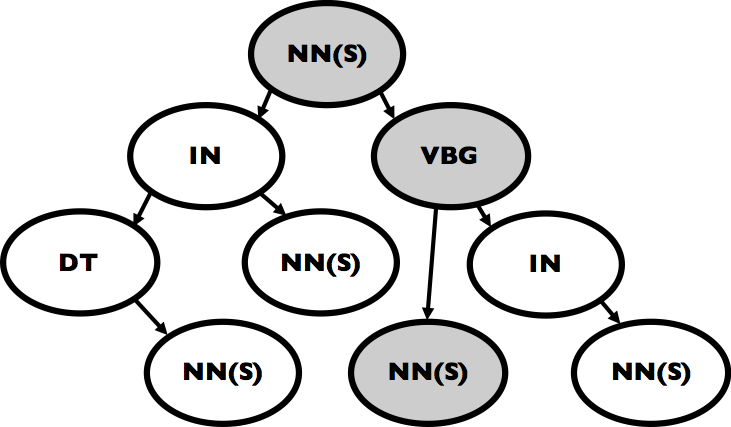
\includegraphics[width=\linewidth]{syntax_tree}
    \end{subfigure}
    \caption{\textit{Floating syntax constraints}. Shown are two 10-syllable phrases (representing the overlap of two states in a 9th-order NHMM) each with its syllable-level POS template (per the Stanford CoreNLP Toolkit). The tree represents a floating word-level POS template constraint. Each path through the tree represents a POS sequence that is valid per the constraint. Each phrase (representing a Markov transition) is either kept or pruned according to whether or not its syllable-level template (when identical consecutive tags are merged) has a valid path through the tree. This is a floating constraint because the POS tags from the constraint are not imposed on specific positions in the syllable-level template. Thus despite having different syllable-level POS templates, both phrases satisfy the constraint via the same path (grey).}
    \label{fig:syntax_tree}
\end{figure}

%We discuss possible non-Markovian solutions to this problem in Section~\ref{abstract_model_description}.

% \subsubsection{A Function for Rhyming}

% Most constraints have fairly straightforward implementations: if a syllable is constrained to be a certain stress, then it either is or it is not; likewise with POS constraints. However, rhyme constraints require a function that, given two syllables, can determine if or how well the syllables rhyme. Several approaches have been taken to this problem. Hirjee \cite{hirjee2010using}. Brown.

% In addition to these approaches, we developed a novel approach that uses linguistic features to analyze rhyme similarity between syllables. Weights for these features were learned using a genetic algorithm trained on data from the Datamuse project.

As training data for our DBTB models we used the Corpus of Contemporary American English (COCA) \cite{davies2009385+}. To improve parsing we selected only complete phrases (as delimited by any non-alphabetic or apostrophe characters) which had a maximum of 30 space-delimited word tokens. POS tagging was performed using the Stanford CoreNLP Toolkit \cite{Manning2014}. Sentence pronunciation was inferred using word pronunciations from the CMU dictionary\footnote{\url{http://www.speech.cs.cmu.edu/cgi-bin/cmudict}} and the CMUSphinx grapheme-to-phoneme converter \cite{Walker2004}. Models were trained on each unique pronunciation of the sentence, with each pronunciation being weighted in the model proportional to the number of pronunciations for the sentence.

We trained five NHMMs (see Table~\ref{tab:model_summaries}). All but one found satisfying solutions. Each model was trained on sentences whose syllable sequence length $l_s$ was $d \leq l_s \leq 30$. The system, implemented in Java 1.8, trained with 24 cores and 256 GB of RAM for 5 hours and 43 minutes.

\begin{table*}
\scriptsize	
\centering
\caption{$d$-order NHMMs with Floating and Dynamic Constraints for Solving the DBTB Problem}
\label{tab:model_summaries}
\begin{tabular}{llllll}
\hline
	& NHMM 1  & NHMM 2   & NHMM 3 & NHMM 4 & NHMM 5 \\ \hline
NHM Order & 4 & 5 & 5 & 6 & 8 \\
NHM Length & 3 & 3 & 4 & 3 & 4 \\
Sequence Length & 6 & 7 & 8 & 8  & 11 \\
Stress Template & {[}011001{]} & {[}0110101{]} & {[}01010010{]} & {[}01101011{]} & {[}01010101010{]} \\
\begin{tabular}[c]{@{}l@{}}Dynamic Rhyme\\ Constraint Positions\end{tabular} & 2\&6 & 2\&7 & 2\&7, 3\&8 & 2\&8 & 2\&10, 3\&11 \\
\begin{tabular}[c]{@{}l@{}}Floating POS\\ Constraint Positions\end{tabular}  & 2-6 & 2-7 & 2-7 & 2-8 & 2-10 \\ \hline
Training Sentences & 3,892,039 & 2,654,884 & 2,654,884 & 2,051,040 & 1,239,850 \\
Training Pronunciations & 366,062,046 & 286,075,704 & 286,075,704 &255,086,072 & 208,330,754 \\ \hline
Solutions Generated & \textbf{30} & 5 & 5 & 4 & \textit{Not Satisfiable}\\
Generated Example                            & \begin{tabular}[c]{@{}l@{}}``a dish of \\ pickled fish''\end{tabular} & \begin{tabular}[c]{@{}l@{}}``a cot and a \\ chamber pot''\end{tabular} & \begin{tabular}[c]{@{}l@{}}``a pillar that \\ was a mirror''\end{tabular} & \begin{tabular}[c]{@{}l@{}}``a mouse or a rat \\ in the house''\end{tabular} & \textit{n/a}\\
Average Novelty & 3.65 & 3.66 & \textbf{4.13} & \textit{3.40} & \textit{n/a }\\
Average Rhyme & 4.18 & \textbf{4.21} & \textit{1.94} & 4.00 & \textit{n/a} \\
Average Rhythm & 3.12 & \textbf{3.30} & \textit{2.13} & 3.16 & \textit{n/a} \\
Average Amusement & \textbf{2.53} & 2.39 & \textit{2.06} & 2.48 & \textit{n/a} \\
Average Likability & 2.51 & 2.66 & \textit{2.17} & \textbf{2.82} & \textit{n/a} \\ \hline
\end{tabular}
\end{table*}

To evaluate the effectiveness of higher-order NHMMs, we performed a qualitative assessment of DBTB solutions generated by our models. We first obtained human-generated solutions by inviting university faculty and students to ``come up with your own novel ending''. We randomly selected 88 DBTB solutions (44 computer-generated and 44 human-generated). We conducted 94 surveys in which participants were asked to rate five DBTB solutions (randomly and evenly sampled from our mixed pool) on Likert scales for novelty, rhyme, rhythm, amusement, and overall likability (each solution thus being rated an average of 5.34 times). Results are shown in Table~\ref{tab:model_summaries} and Figure~\ref{fig:results}.

\begin{figure} 
\centering
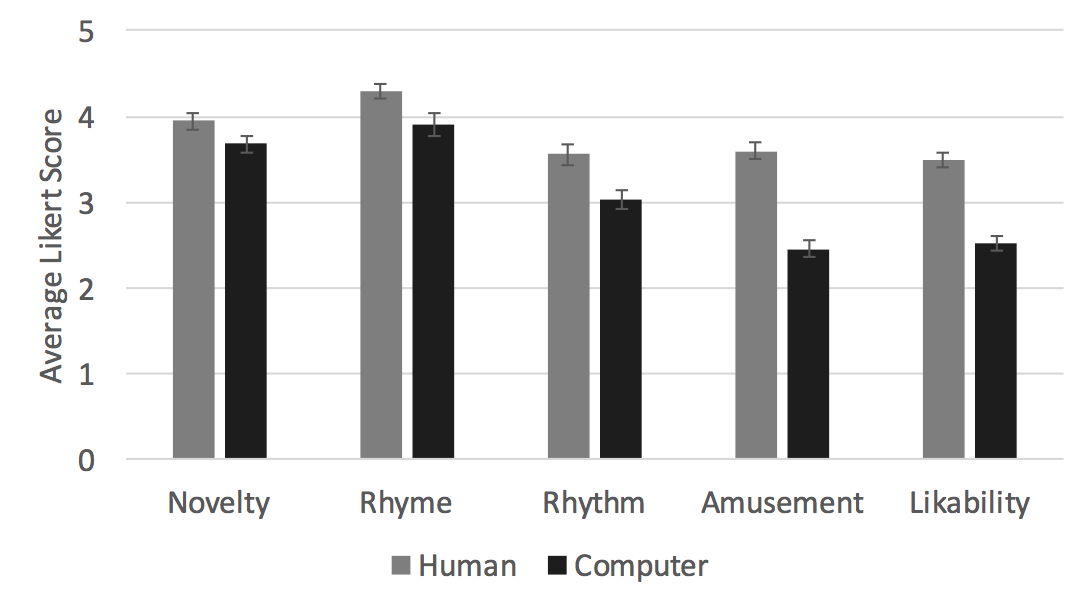
\includegraphics[width=\linewidth]{evaluative_results}
\caption{\textit{Qualitative evaluation.} Results of 470 survey responses rating human- and computer-generated solutions to the DBTB problem. Error bars represent standard error.}
\label{fig:results}
\end{figure}

The top five highest-scoring computer-generated solutions, their scores (averaged over the 5 criteria), and the NHMM that created them were:
\begin{itemize}
\item ``a way out of the bay'' - 4.04 - NHMM 1
\item ``a place in Chevy Chase'' - 3.85 - NHMM 1
\item ``a sign of the decline'' - 3.8 - NHMM 1
\item ``a scar shaped like a star'' - 3.75 - NHMM 1
\item ``a stream that wound like a dream'' - 3.74 - NHMM 2
\end{itemize}
%\noindent More examples can be found at twitter.com/botbythebay. 

We found that the novelty scores of human-generated solutions outscored computer-generated solutions by a margin of 0.25. The rhyme scores were also very competitive, with the delta (0.38) being partially explained by our failure to consider the matching of syllable onsets in multisyllabic words (e.g., ``pillar'',``mirror'') in Model 3. We hypothesize that the delta observed in the rhythm score may be due to the confounding variables of rhyme and grammaticality. For example, the poor rhyming performance of Model 3 (the only model with multisyllabic rhymes) may have carried over into the ratings for other aspects of Model 3 solutions. Likewise it seems a reasonable hypothesis that, although poor grammar does not affect rhythm, it may nonetheless be perceived to affect the rhythm; however, we did not include grammaticality in our assessment. The amusement and likability scores, with which the computer struggled most, may have been a affected by the genre-appropriateness of some of the computer-generated solutions (e.g., ``a flood of spurting blood'', ``an orphan and an abortion'') and would likely be improved if we had chosen a different training dataset.

\subsection{Floating Semantic Constraints in Haiku}

To demonstrate the generality of floating constraints, we designed and applied two different syllable-level NHMMs on the COCA fiction corpus \cite{davies2009385+}. The first was a 5th-order NHMM of length 13 with a \textit{nature}-themed floating semantic constraint applied over the first 5 syllables. The second was a 4th-order NHMM of length 14. In this model we applied a floating word-level POS template constraint (similar to those described for the DBTB models) over the last 5 syllables of each line. Each line-specific constraint had a syntax tree populated with word-level POS templates parsed from corresponding lines in a database of existing haiku. 

We also imposed a \textit{beauty/earth}-themed floating semantic constraint over the last 4 syllables using \citeauthor{mikolov2013distributed}'s word2vec approach  (\citeyear{mikolov2013distributed}) to ascertain semantic relatedness between words. In both models, each line was constrained to start and end with word-starting and word-ending syllables. Of the two models, the first found several interesting \textit{objets trouv\'es} whereas the second generated novel compositions (see Figure~\ref{fig:haiku}).

\subsection{Floating Stress Constraints in Prosody}

For generating prosodic rhythm, we designed a 4th-order NHMM over rhythm tokens of length 6 to generate suitable rhythms for the lyrics ``No more monkeys jumping on the bed''. We trained the model on lyric/rhythm sequences from the Wikifonia dataset. Given a stress template of [111010101] (per the CMU pronunciation dictionary), the model imposes floating stress constraints requiring 80\% of syllable stresses to be matched appropriately to emphasized rhythmic positions (one constraint over the first five syllables and another over the last four syllables). The model also has 4/4 floating time signature constraints at all positions (see Figure~\ref{fig:monkeys}). 

\begin{figure}
\centering
\begin{subfigure}[b]{.5\linewidth}
\centering
\textit{trees lifted themselves \\
up and snapped to attention \\
with seasonal fire \\}
\end{subfigure}
\begin{subfigure}[b]{.45\linewidth}
\centering
\textit{the trajectory \\
of the individual \\ 
nature and history \\}
\end{subfigure}

\caption{\textit{Haikus}. These haikus are generated from syllable-level NHMMs with floating constraints. (Left) An \textit{objet trouv\'e} found using a 5th-order NHMM with a \textit{nature}-themed floating semantic constraint. (Right) An original haiku generated from a 4th-order NHMM with floating word-level POS template constraints and a \textit{beauty/earth}-themed floating semantic constraint.}
\label{fig:haiku}
\end{figure}

\begin{figure}
    \centering
%     \begin{subfigure}[b]{\linewidth}
%         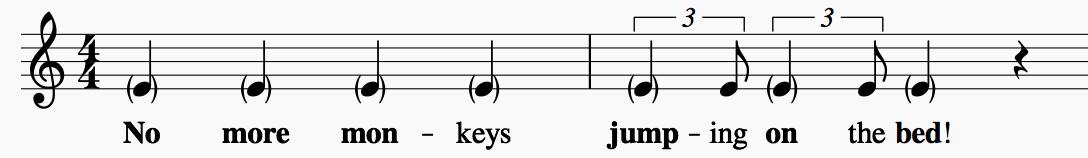
\includegraphics[width=\linewidth]{monkeys_1}
%     \end{subfigure}
    \begin{subfigure}[b]{\linewidth}
%         \vspace{.4cm}
        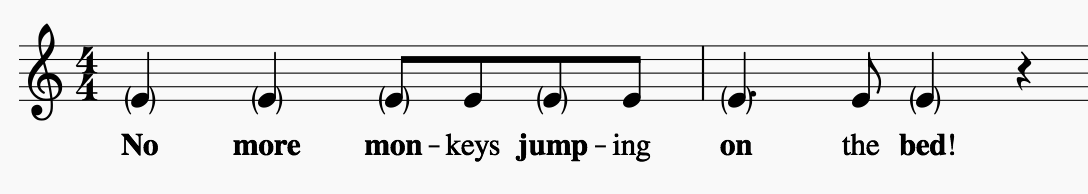
\includegraphics[width=\linewidth]{monkeys_2}
    \end{subfigure}
    \begin{subfigure}[b]{\linewidth}
%     	\vspace{.4cm}
        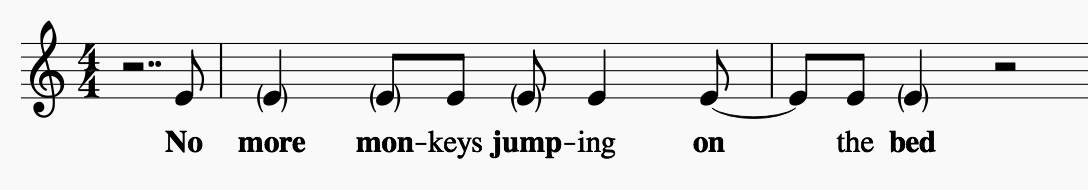
\includegraphics[width=\linewidth]{monkeys_3}
    \end{subfigure}
    \caption{\textit{Prosodic rhythm for lyrics}. Given the lyric ``No more monkeys jumping on the bed!'', we used a 4th-order NHMM over rhythm tokens to generate prosodic rhythms like those shown here. Stressed syllables are \textbf{bold} and notes in emphasized rhythmic positions are in parentheses.}
    \label{fig:monkeys}
\end{figure}

% \subsection{A High-Order vs A Variable-Order Markov Model} 
% \label{var_order_model}

% Besides the obvious advantages of using a variable-order Markov model, such a model is required to maintain equivalence between word-level and syllable-level model inasmuch as there are a variable number of syllables per word. As discussed above, the transition information in a $d$-order Markov model on word tokens gets diluted when converting to a syllable-level $d$-order Markov model (for $d > 1$) to varying extents depending on the specific prefix.

% It should be noted, however, that variably elongating the order for syllable prefixes in order to maintain the same transition info in a word model of any particular order is of questionable priority. In the case of the DBTB and similar problems, syllable prefixes are already (too) long in order to encompass rhyming syllable positions. Any variable-order syllable model would have to extend beyond that length, resulting in an even stronger trend towards memorizing the training set.

% Of larger philosophical significance is the fact that the information contained in word model is already of arbitrary value inasmuch as $d$-grams having varying expectation values. The prefix ``I love'' contains little information about what follows as compared with the prefix ``National Basketball'' which with high probability will be followed by ``Basketball Association''. Words might thus in some sense be considered arbitrary breaks in the syllable stream. It is of marginal value therefore to go to any great lengths when converting to a syllable model to preserve the (variable) expectation of prefix-prefix transitions in a word model.

% \subsection{Compromising Length, Order, and Constraints}

\section{Discussion}

The number of satisfying solutions to any given problem fluctuates significantly as a function of a model's length, order, and the cardinality/severity of its constraints. In practice this results in having to make compromises: adding constraints requires decreasing the order; increasing the order requires decreasing the length; increasing the length requires lowering a particular constraint threshold; and so on.

One ramification of this is a variation of the no free lunch theorem: different model settings will generate a different subset of the ideal solutions. In our study we tried several different permutations to find that which we felt worked best on average and which produced a reasonable number of good solutions. But there are likely many more good solutions we might have found via other permutations.

A second ramification of the need for compromise is that it presents several novel challenges to be solved: how can we find the optimal parameters for length, order, and constraints? Can constraints be prioritized or made more flexible so as not to over-prune the model? Some of the answers to these questions may require domain-specific knowledge; however, ideally we may find more generalizable solutions.

In this work we have demonstrated the implementation of higher-order NHMMs and presented two new classes of constraints (floating constraints and dynamic constraints) that are uniquely accessible to such models. We have presented several useful optimizations for implementing NHMMs. We have explored the advantages of syllable-level models for text generation. We have demonstrated the efficacy of these findings in several domains, including its application to the Down by the Bay problem.

\chapter{Sequential Structure Inference Via Multiple Self-Alignment}

\emph{We plan to submit this paper to the 2018 Association for the Advancement of Artificial Intelligence Conference on Artificial Intelligence}
\section{Introduction}

Human-level concept learning relies on the ability to model artefacts at increasing levels of abstraction \cite{lake2015human}. In visual imagery, pixels form strokes which form shapes which form objects. In natural language, letters make words which make phrases which make sentences. The ability to learn high-level features is critical to an effective model of the domain, either for discrimination or generation.

Often features of interest are abstract, that is they are not explicitly represented in an artefact description. In poetry or lyrics, features such as rhyme scheme are not usually labeled; however, even beginning readers are capable of identifying intentionally rhymed phrasing \cite{englemann1974distar}. In music, features such as verse-chorus segmentation and repeated motifs are infrequently labeled but are nonetheless readily inferred by even non-musicians from what \textit{is} represented (e.g., chords, melody). This structure significantly relates to meaning \cite{Nunes2014}, and although audiences will find structure even where it was not intended, they readily express criticism of artefacts in which they perceive little or no structure. Human-level reasoning about artefacts and domains hinges on the ability to recognize structure within \textit{primitive} features (i.e., features that are labeled) from which \textit{abstract} structural features can then be inferred.  Such features are helpful for evaluating, classifying, comparing, and/or generating structured artefacts \cite{Bodily2017ComputationalLearning}. In addition, style-transfer and cross-domain translation of ideas is better facilitated by the ability to elucidate abstract structural representation \cite{lecun2015deep}.

Much related work exists to finding structure in sequential data. \citeauthor{meredith2002algorithms} \cite{meredith2002algorithms} discover patterns of multidimensional repetition using maximal translatable patterns (MTPs). \citeauthor{collins2010comparative} \cite{collins2010comparative} follow up on this work with a pattern discovery algorithm called SIACT to discover translational patterns in baroque keyboard works which they later also use in extracting patterned repetitions in music \citeauthor{collins2017computer} \cite{collins2017computer}. \citeauthor{lattner2015pseudo} \cite{lattner2015pseudo} use bootstrapping in feed-forward neural networks to perform unsupervised melody segmentation. Other work has approached the musical sequence segmentation problem using restricted Boltzmann machines \citeauthor{lattner2015probabilistic} \cite{lattner2015probabilistic}.

We present a novel approach to inferring abstract structural features that uses genetic algorithms to determine viewpoint-specific scoring functions for structural sequence alignment. The approach is readily applicable across domains where structure can be modeled in terms of self-similarity (e.g., bioinformatics, natural language, and audio signal processing). As a concrete example for the purposes of demonstration, we examine the inference of abstract structure in lyrical, sectional-form music lead sheets, with the goal of identifying patterns of repetition within viewpoints (c.f., \cite{conklin1995multiple}) and at the more abstract levels of detecting chorus and verse structures.

Identifying \textit{identical} structural patterns is trivial for humans and computers alike. However, humans identify structure extremely well even when repetitions are \textit{not} identical. In music, for example, a human listener readily identifies melodic and harmonic similarity between verses despite variation in pitch, rhythm, and lyrics. Alignment algorithms---such as the Needleman-Wunsch (NW) \cite{needleman1970general} or Smith-Waterman (SW) \cite{smith1981identification} algorithms---have traditionally been used to align similar non-identical sequences in bioinformatics and natural language, although their implementation usually focuses on finding similarity \textit{between} rather than \textit{within} sequences (e.g., see Figure~\ref{fig:swexample}). Furthermore, sequence alignment algorithms have typically been used on sequences of discrete tokens belonging to finite-length alphabets, making it easy to derive static scoring matrices (e.g., PAM \cite{dayhoff197822} and BLOSUM \cite{henikoff1992amino}) for defining a pairwise scoring function.

\begin{figure*}
	\centering
	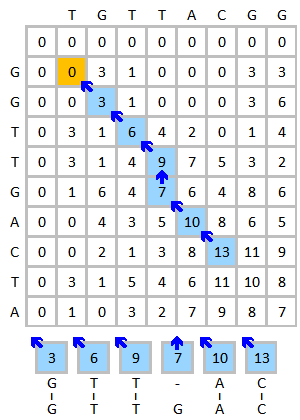
\includegraphics[width=.6\linewidth]{swexample}
    \caption{\label{fig:swexample}\textit{Traditional Smith-Waterman Alignment Example}. Shown is an example of DNA alignment using the Smith-Waterman algorithm. The highest scoring alignment is derived starting from the highest scoring cell in the alignment matrix and then backtracking along the path taken to arrive at that cell until the path reaches a cell with a score of 0. The alignment suggests which DNA bases from each DNA sequence are matching. We use an analogous method to find matching sequence events in music. Image courtesy of Wikimedia Commons.}
\end{figure*}

%Dan dropped
%Many domains, such as graphic art and signal processing, are represented as continuous sequences with abundant features that make enumerating the event space unreasonable. Furthermore, although there is significant interest in finding patterns \textit{between} artefacts in these domains, many important abstract features exist only as a result of patterns \textit{within} single artefacts. Therefore, though sequence alignment may serve well to find regions of self-similarity, several significant adaptations are required to elucidate structure within artefacts in continuous, feature-rich domains.

\section{Methods}

The fundamental premise of the approach is that structure in an artefact exists by virtue of self-similarity. In music, the verse-chorus structure is a product of similarity across viewpoints such as melody, chords, and (for choruses) lyrics.

A primary challenge in alignment is determining alignment parameters. Sequence alignment algorithms generally require defining a gap or \textit{insertion/deletion} cost, $G$, as well as a scoring function $s(x_1,x_2)$ for two arbitrary sequence elements $x_1$ and $x_2$. These definitions are non-trivial because they can dramatically affect the resulting alignment.

In traditional alignment domains, the definition of a scoring function is relatively straight-forward because sequence elements are easily represented using a (relatively) small alphabet. In this case the scoring function usually consists of a simple lookup table where values in the table represent the likelihood that one element is aligned with any other element \cite{henikoff1992amino}.

However in considering the alignment of musical sequences, a sequence element or \textit{event} is significantly more complex for a few reasons. First, music---both acoustic and symbolic---represents a continuous sequence of sound. It may be discretized at various intervals (e.g., acoustic sampling rates, metrical beats, etc.), but how the sequence is discretized will directly impact the ability to detect patterns across various viewpoints. Because the time and space required per alignment increase exponentially with the sampling rate, we chose a sampling rate of 2 events per beat.

The second complexity involved in a musical sequence element is that, even given a particular discretization of musical events, a single event (e.g., Figure~\ref{fig:music_sequence}) is composed of many different viewpoints. Even if we consider a relatively simple representation of music such as a lyrical lead sheet, combining the number of features to consider per musical event with their respective ranges is sufficient to define a intractable number of unique musical events (Table~\ref{tab:features}).

\begin{table*}
\footnotesize
\centering
\renewcommand{\arraystretch}{1.1}
\begin{tabular}{m{1.3in}|m{2.5in}|m{1.2in}|m{1in}}
\textbf{Event Feature} & \textbf{Description} & \textbf{Range} & \textbf{Feature Value for $E$ in Figure~\ref{fig:music_sequence}} \\ \hline
$is\_rest(E)$ & $True$ if $E$ occurs during a rest & $[True,False]$ & $False$ \\ \hline
$pitch(E)$ & the MIDI note value being voiced at $E$ & \begin{tabular}{@{}l@{}}[0,127] \\ ($\varnothing$ if $is\_rest(E)$)\end{tabular} & 69 \\ \hline
$measure(E)$ & the measure in which $E$ occurs (0-based) & $\mathbb Z_{> 0}$ & 3 \\ \hline
$beat(E)$ & the offset in beats within measure $measure(E)$ (0-based) & $\mathbb R_{> 0}$ & 0.5 \\ \hline
$duration(E)$ & the duration in beats of the note or rest being voiced at $E$ & $\mathbb R_{> 0}$ & 2.5 \\ \hline
$is\_note\_onset(E)$ & $True$ if the measure and beat of the onset of the note or rest being voiced at $E$ equals $measure(E)$ and $beat(E)$ & $[True,False]$ & $True$ \\ \hline
$lyric(E)$ & the lyric being sung at $E$ & Set of all valid syllables $\cup$ $\varnothing$ & ``try'' \\ \hline
$is\_lyric\_onset(E)$ & $True$ if the measure and beat of the onset of the lyric being voiced at $E$ equals $measure(E)$ and $beat(E)$ & $[True,False]$ ($\varnothing$ if $lyric(E)=\varnothing$) & $False$\\ \hline
$harmony(E)$ & the harmony (represented using chord symbols) being voiced at $E$ & Set of all valid chord symbols $\cup$ $\varnothing$ & F \\ \hline
$is\_harmony\_onset(E)$ &  $True$ if the measure and beat of onset of the harmony being voiced at $E$ equals $measure(E)$ and $beat(E)$ & $[True,False]$ ($\varnothing$ if $harmony(E)=\varnothing$) & $False$
\end{tabular}
\caption{\label{tab:features} Features for a music sequence event}
\end{table*}

\begin{figure*}
	\centering
	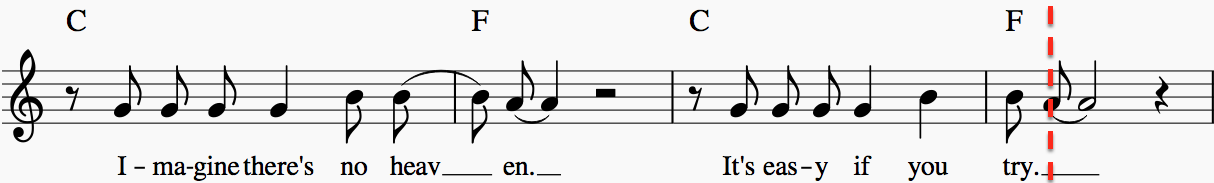
\includegraphics[width=.9\linewidth]{music_sequence}
    \caption{\label{fig:music_sequence}\textit{Example of a music sequence event}. Musical sequences are non-discrete and thus events must be sampled. Table~\ref{tab:features} describes the features and feature values for the event sampled at the dotted red line.}
\end{figure*}

%Dan dropped
%In practice our goal is to find structure across a subset of these features. For example, our intuition might suggest that structural motifs in a song's lyrics depend primarily on an event's lyric content, lyric onset information, and measure/beat (for evaluating temporal spacing). We might struggle, however, to know the relative importance of each of these features in scoring similarity. The lyric scoring function must also score pairs of events in which no lyric is sung or perhaps where no note is being played (rest), though intuition about what these scores should be may also be lacking.

%Dan dropped
%Rather than attempting to guess how each of these features should be weighted, we turn to a machine learning solution in which the computer via a genetic algorithm (GA) is able to find the weights for each of these features which, when used in the scoring function, properly aligns musical subsequences that are known to be similar. Each primitive viewpoint requires its own scoring function and its own training of weights. These functions and weights can then be combined to find abstract structural features \textit{across} primitive viewpoints through the definition of a combined alignment scoring function, effectively \textit{learning-to-learn} \cite{lake2015human}.

\subsection{Multiple Smith-Waterman Self-Alignment}

A traditional NW global sequence alignment is a dynamic programming algorithm \cite{needleman1970general}. For a sequence $a = (a_1,\cdots,a_n)$, let $a'=(a_1,\cdots,a_{n-1})$. The optimal score $S(a,b)$ for the alignment of sequences $a$ and $b$ (with lengths $|a|$ and $|b|$) is defined as a function of the optimal scores for subalignments of $a$ and $b$:
\[
S(a,b) =
\begin{cases}
|a| * G & \text{if } |b| = 0 \\
|b| * G & \text{if } |a| = 0 \\
\text{max}(S(a',b) + G, \\
\quad S(a,b') + G, & \text{otherwise} \\
\quad S(a',b') + s(a_{|a|},b_{|b|}))
\end{cases}
\]
\noindent where $G$ represents the cost of inserting a gap into the alignment and $s(a_{|a|},b_{|b|})$ represents a \textit{pairwise scoring function} which evaluates to a score representative of the cost of aligning the element $a_{|a|}$ with $b_{|b|}$. Some variations (including our own) differentiate between a \textit{gap open cost}, $G_o$, and a \textit{gap extend cost}, $G_e$, where the former is used the first time a gap is inserted and the latter is used for subsequent, consecutive gaps. In this manner the presence and length of a gap can be penalized independently. In practice, a NW alignment sequentially fills in a $(|a|+1)\times(|b|+1)$ matrix, $M$, where the value $M(i,j)$ at the $i$th row and $j$th column represents $S((a_1,\cdots,a_{i-1}),(b_1,\cdots,b_{j-1}))$ (where if $i=0$ or $j=0$ the corresponding sequence evaluates to the empty sequence). The global alignment score is the value of $M(|a|+1,|b|+1)$. The alignment is produced by starting at position $(|a|+1,|b|+1)$ and tracing back through the matrix according to the cells which were used (in the max function) in computing the current cell's value: moving diagonally from $(i,j)$ corresponds to aligning $a_i$ with $b_j$; moving up aligns $a_i$ with a gap; and moving left aligns $b_j$ with a gap. Backtrack continues as long as $i>0$ and $j>0$. 

The SW local alignment algorithm alters aspects of the NW global alignment algorithm to find the highest scoring subsequence alignment between two sequences \cite{smith1981identification}. Modifications are primarily three-fold. First, $S(a,b)$ is additionally constrained to be non-negative, essentially allowing the algorithm to discover the beginning of the optimal alignment anywhere in the alignment matrix $M$. Second, the local alignment score (for the optimal local alignment) is the maximum value in $M$. The row $i$ and column $j$ where this value appears mark the termination of the local alignment. Backtracking proceeds as in the NW algorithm as long as $M(i,j) > 0$.

We are interested in locally aligning musical phrases. We, however, are interested in more than simply the optimal local alignment; we would like to find all significant local alignments. We thus further adapt the SW algorithm to achieve what we call a \textit{multiple Smith-Waterman} (MSW) \textit{self}-alignment. In this variation, we find multiple backtrack points in $M$. To do this we define a \textit{local maximum threshold}, $\tau$, and a \textit{minimum event match distance}, $\epsilon$, such that $M(i,j)$ is a local maximum iff $M(i,j) \geq \tau$ and $M(i,j) \geq M(k,l)$ for $\forall k = i\pm\epsilon$ and $\forall l = j\pm\epsilon$. Backtracking then proceeds as in the SW algorithm. Because we are doing self-alignment, we need only compute the upper diagonal of $M$ (i.e., $j \geq i$). We are also not interested in alignments that are close to the diagonal (i.e., that represent the alignment of an event with itself or close neighbors). We therefore only compute $M$ where $j \geq i + \epsilon$ (see Figure~\ref{fig:alignment_example}). For our implementation, $\epsilon = 4$.

\begin{figure}
\centering
	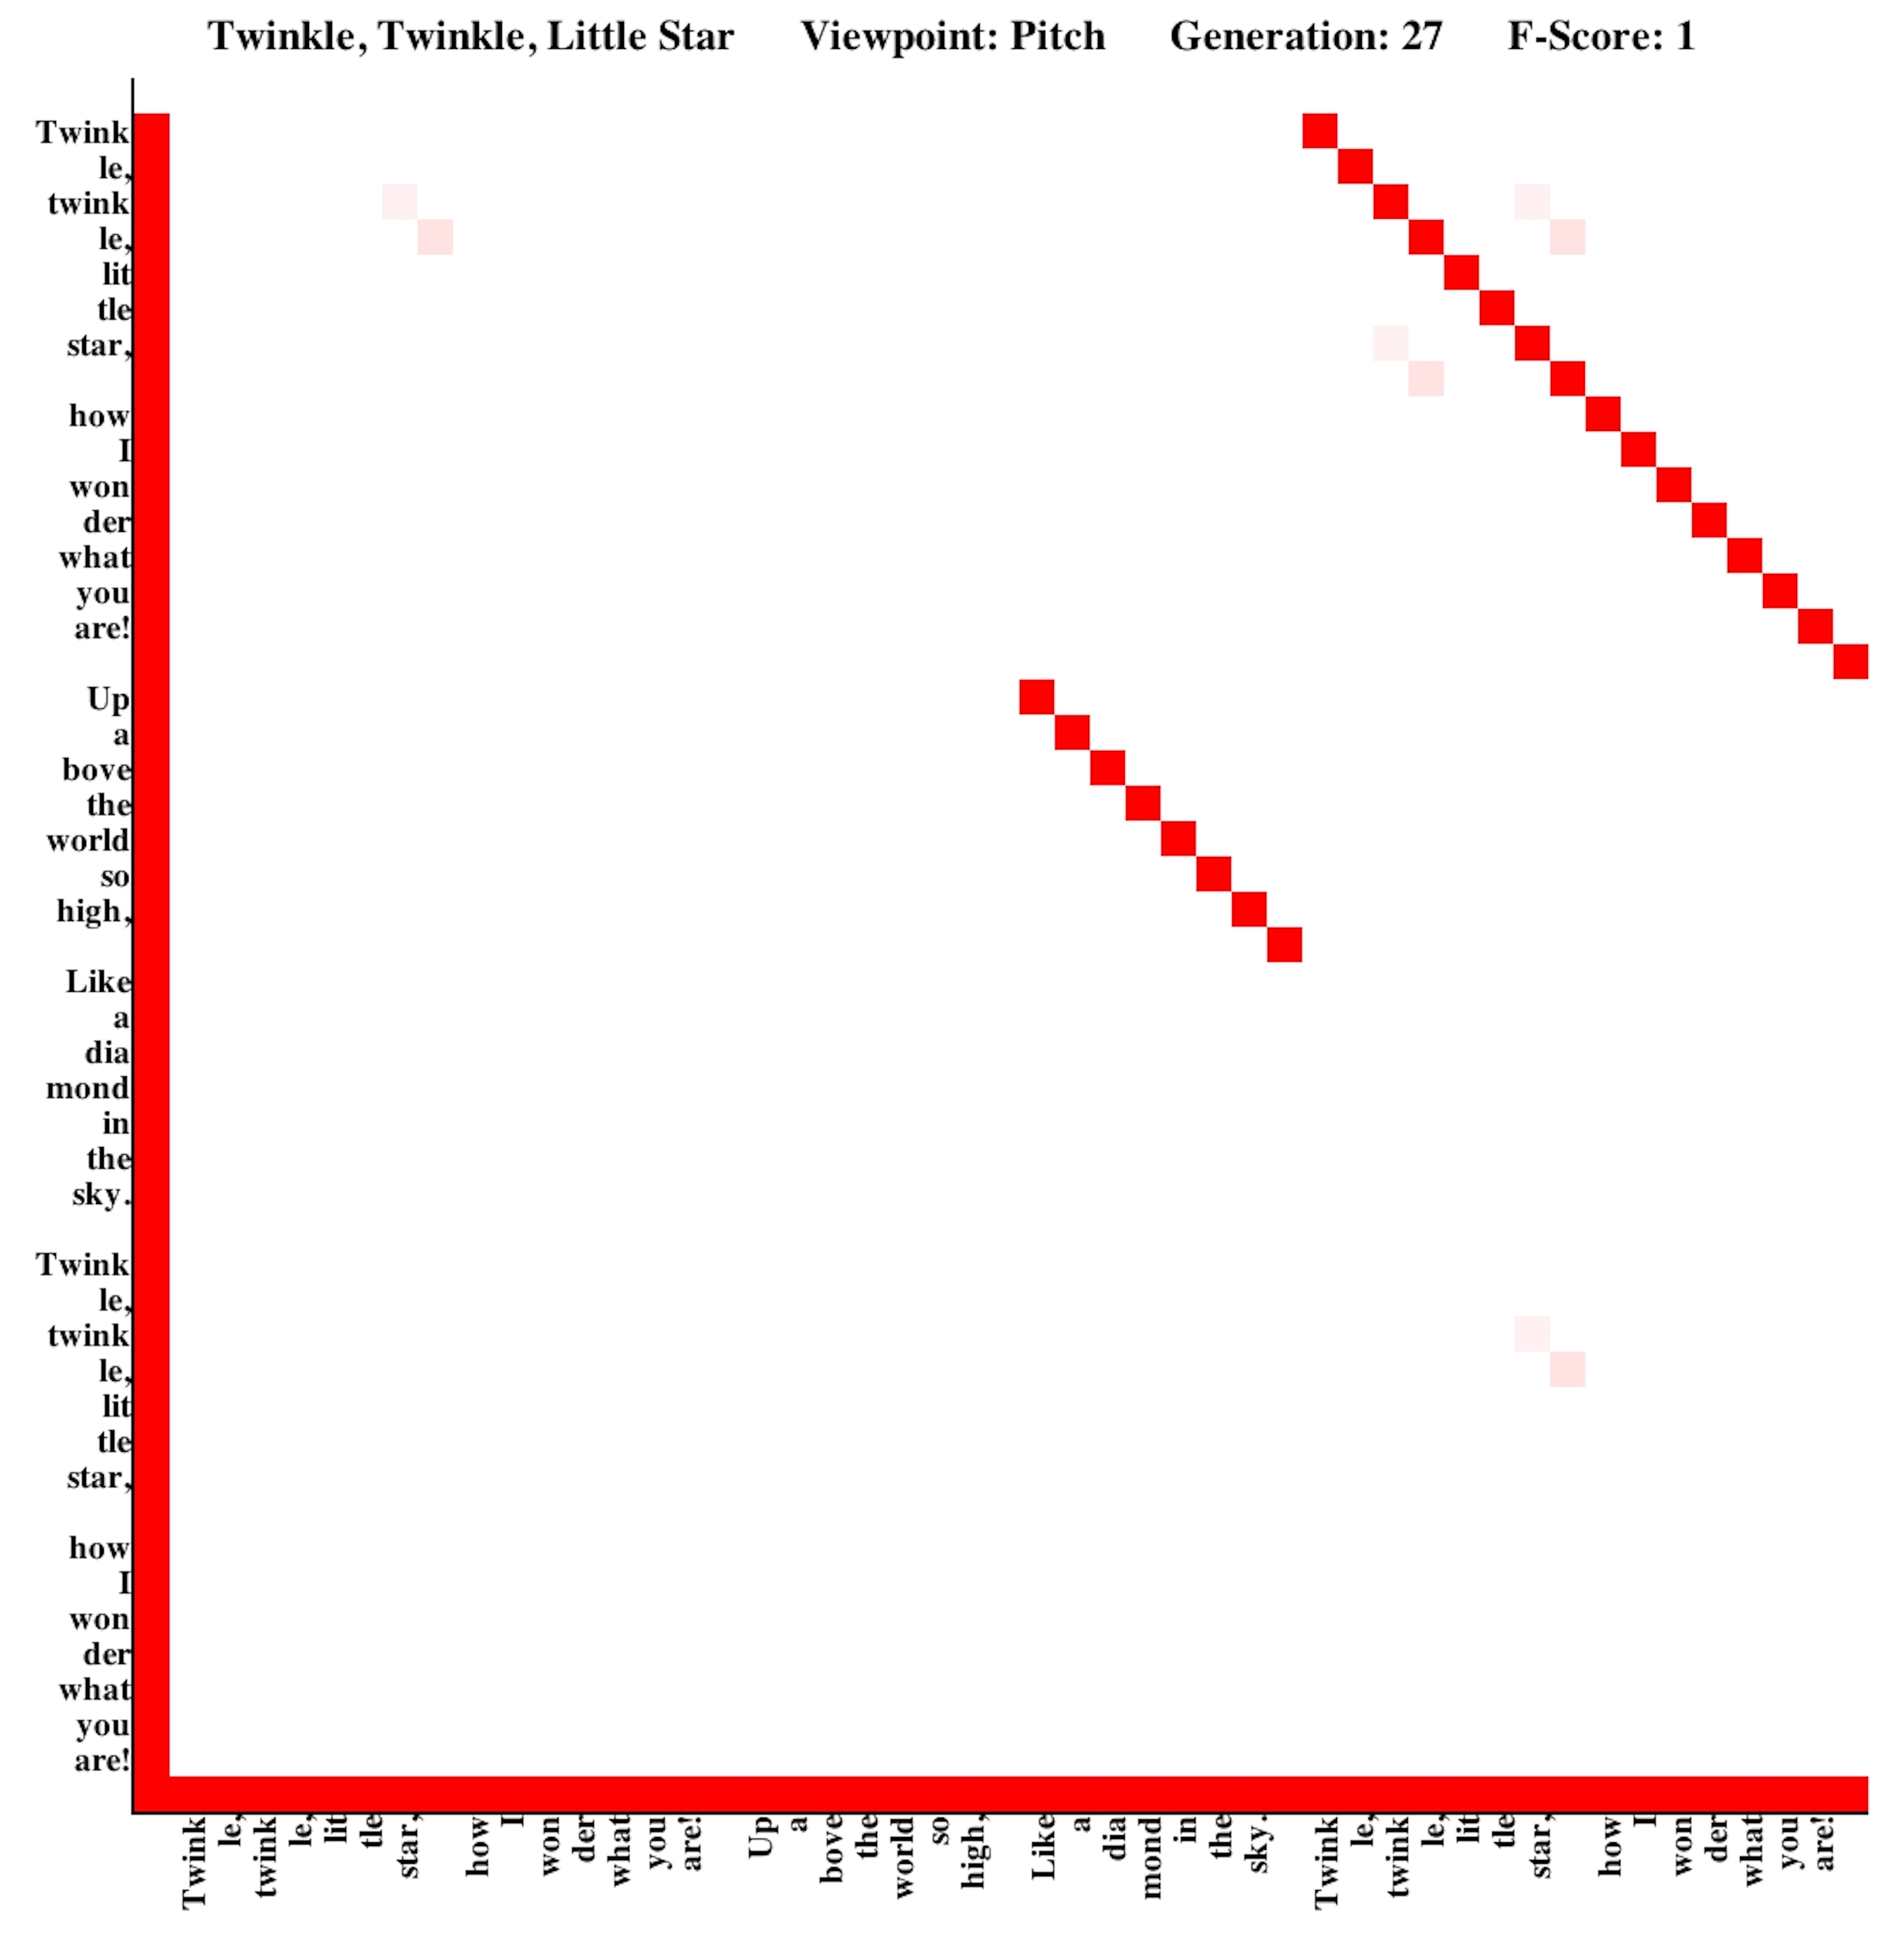
\includegraphics[width=.7\linewidth]{Twinkle__Twinkle__Little_Star_gen27_id137_pitch}

    \caption{\label{fig:alignment_example}\textit{Finding pitch structure via sequence alignment}. Representing the song \textit{Twinkle, Twinkle, Little Star} as a sequence of discrete events, we align the song against itself using a multiple Smith-Waterman alignment and a pitch-specific pairwise scoring function. The longer red diagonal represents the repetition of pitch between the two choruses in the song whereas the smaller diagonal represents repetition of pitch within the bridge section. Weights for the pairwise scoring function are learned via genetic algorithm (see Figure~\ref{fig:learning_weights}). In this example, 27 generations were required to find weights which maximize the fitness function (F-score).}
\end{figure}

\subsection{Genetic Algorithm Parameters}

Given this general approach, the challenge becomes properly defining the pairwise scoring function $s(a_i,b_j)$ and the general alignment parameters $G_o$, $G_e$, and $\tau$. We describe several viewpoint-specific definitions for $s(a_i, b_j)$ below, each of which defines several scoring function parameters. These viewpoint-specific parameters, along with the general alignment parameters, are learned via GA (see Figure~\ref{fig:learning_weights}).

\begin{figure*}
\centering
\newcommand{\colwidth}{1.1in}
\setlength\tabcolsep{2pt} % default value: 6pt
\newcolumntype{D}{ >{\centering\arraybackslash} m{\colwidth} }
\begin{tabular}{DDDDDDD}
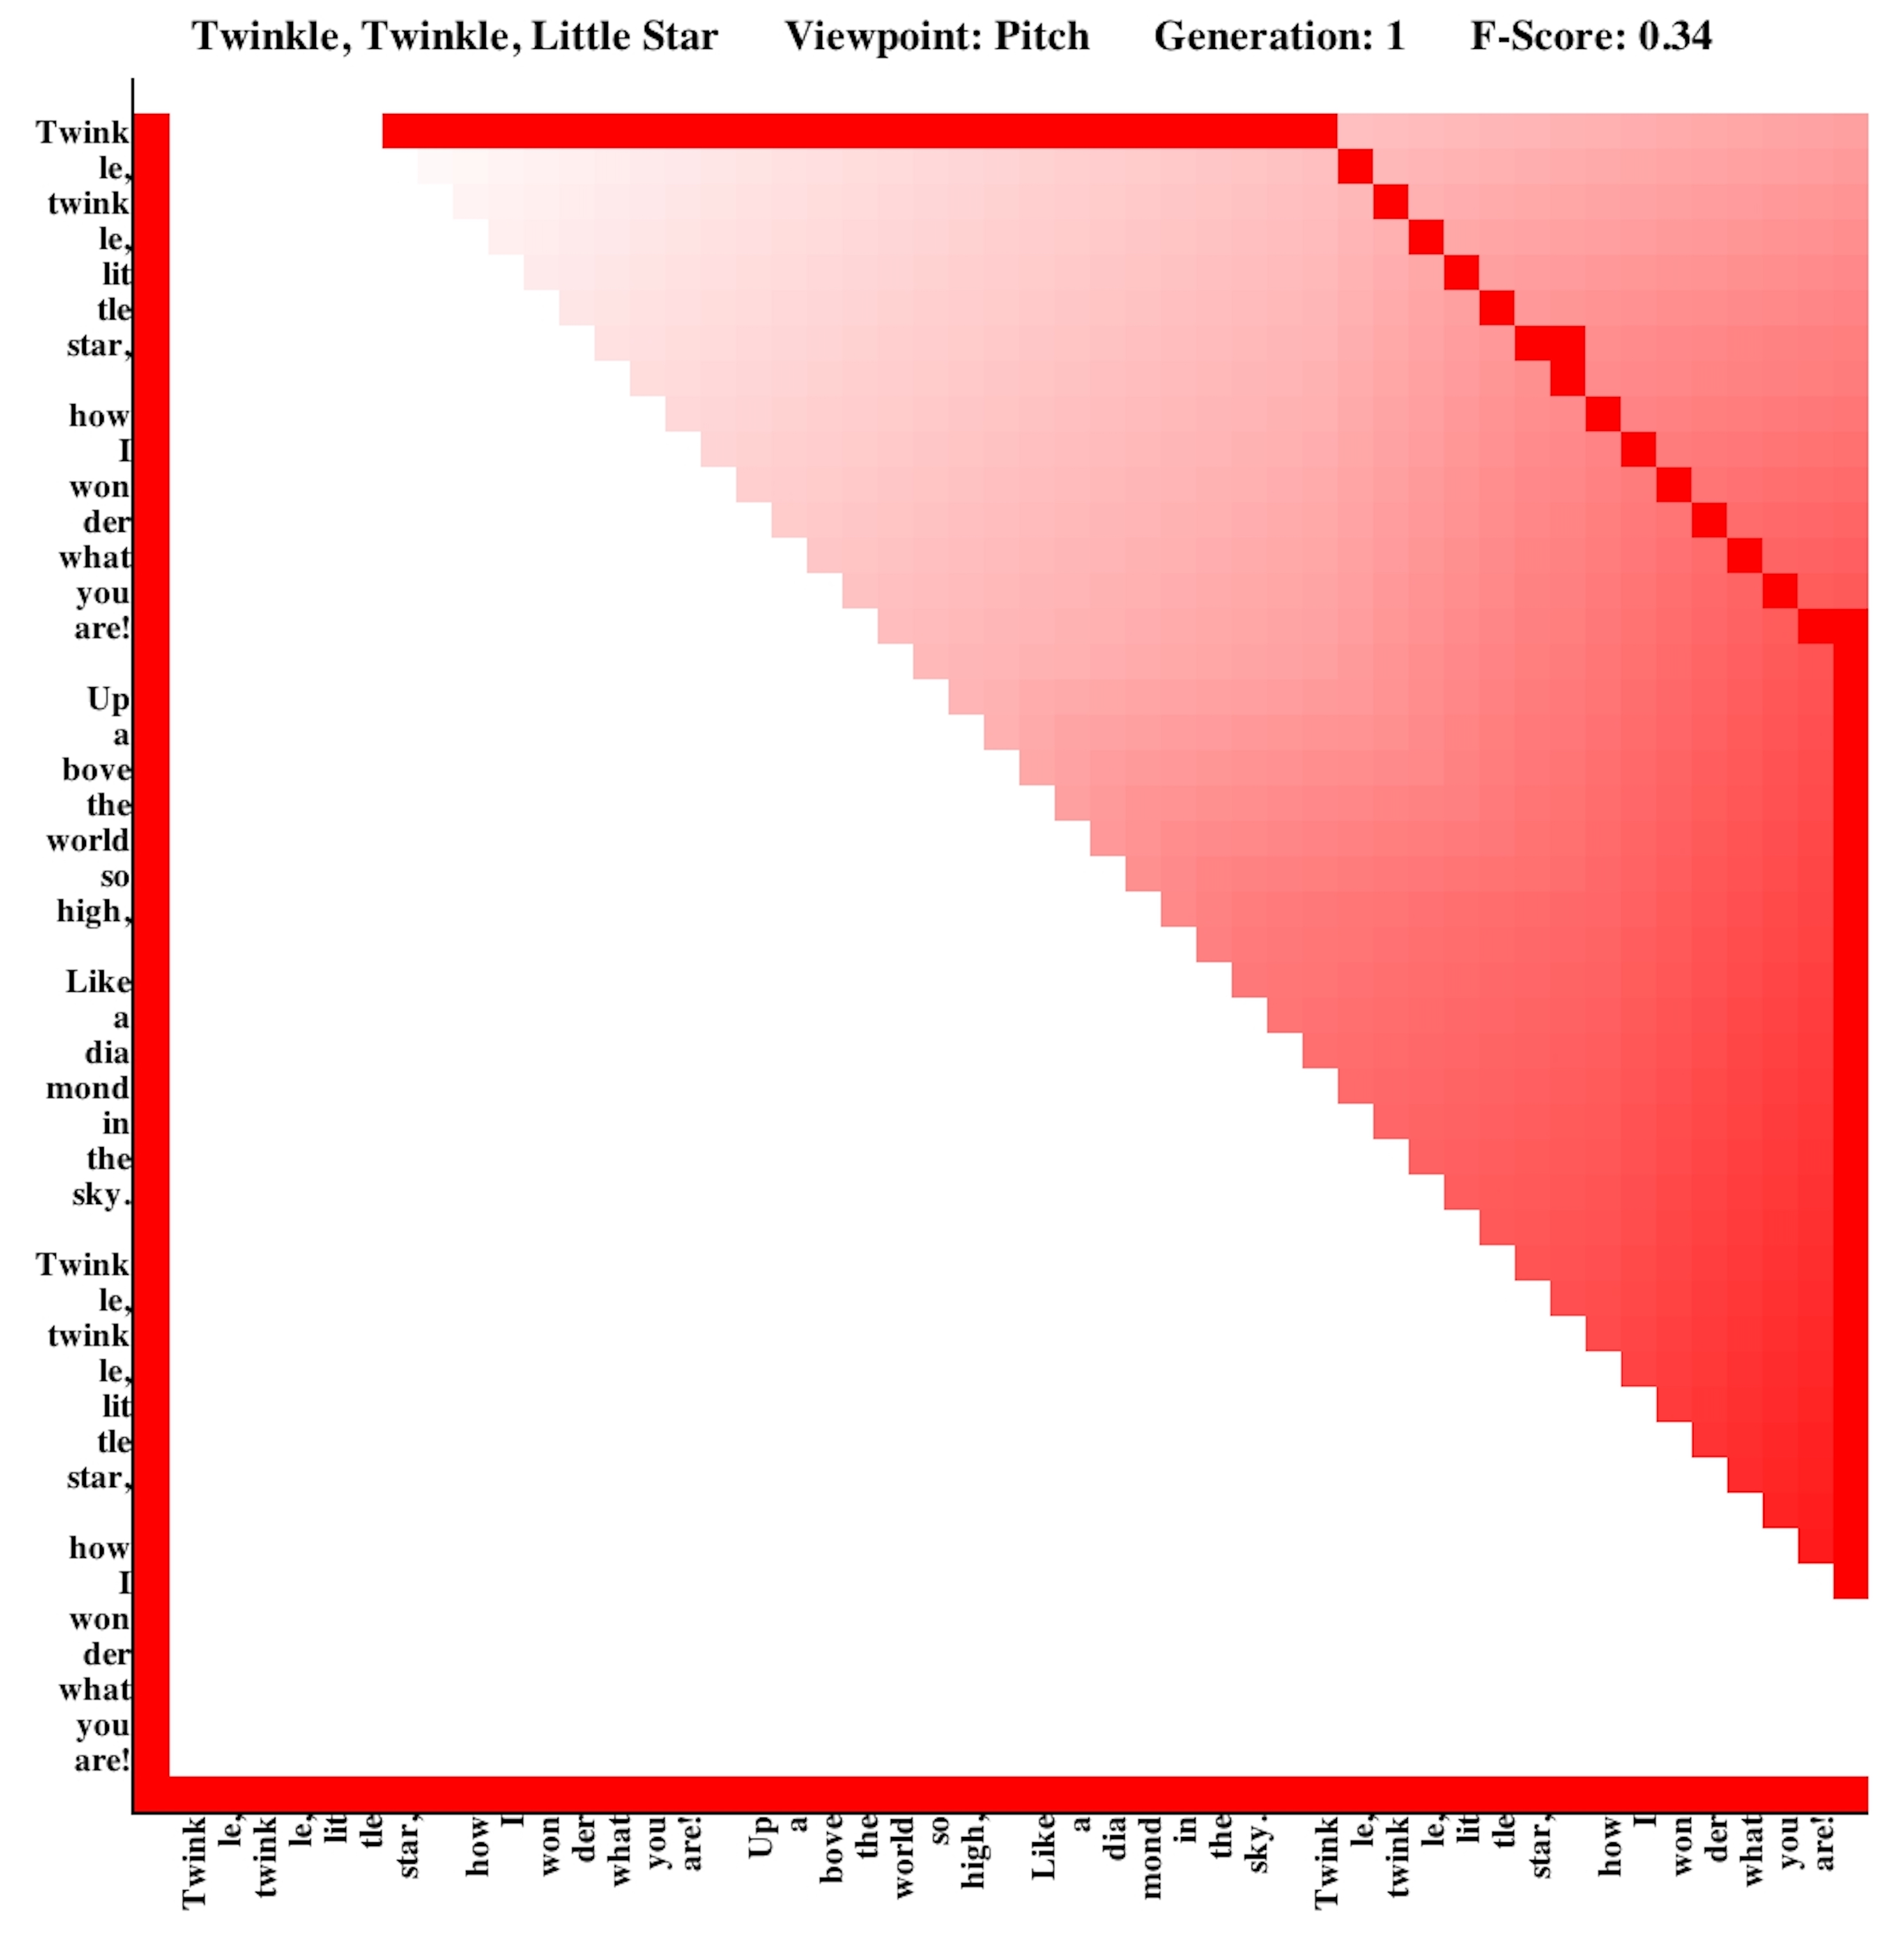
\includegraphics[width=\colwidth]{Twinkle__Twinkle__Little_Star_gen1_id0_pitch} & 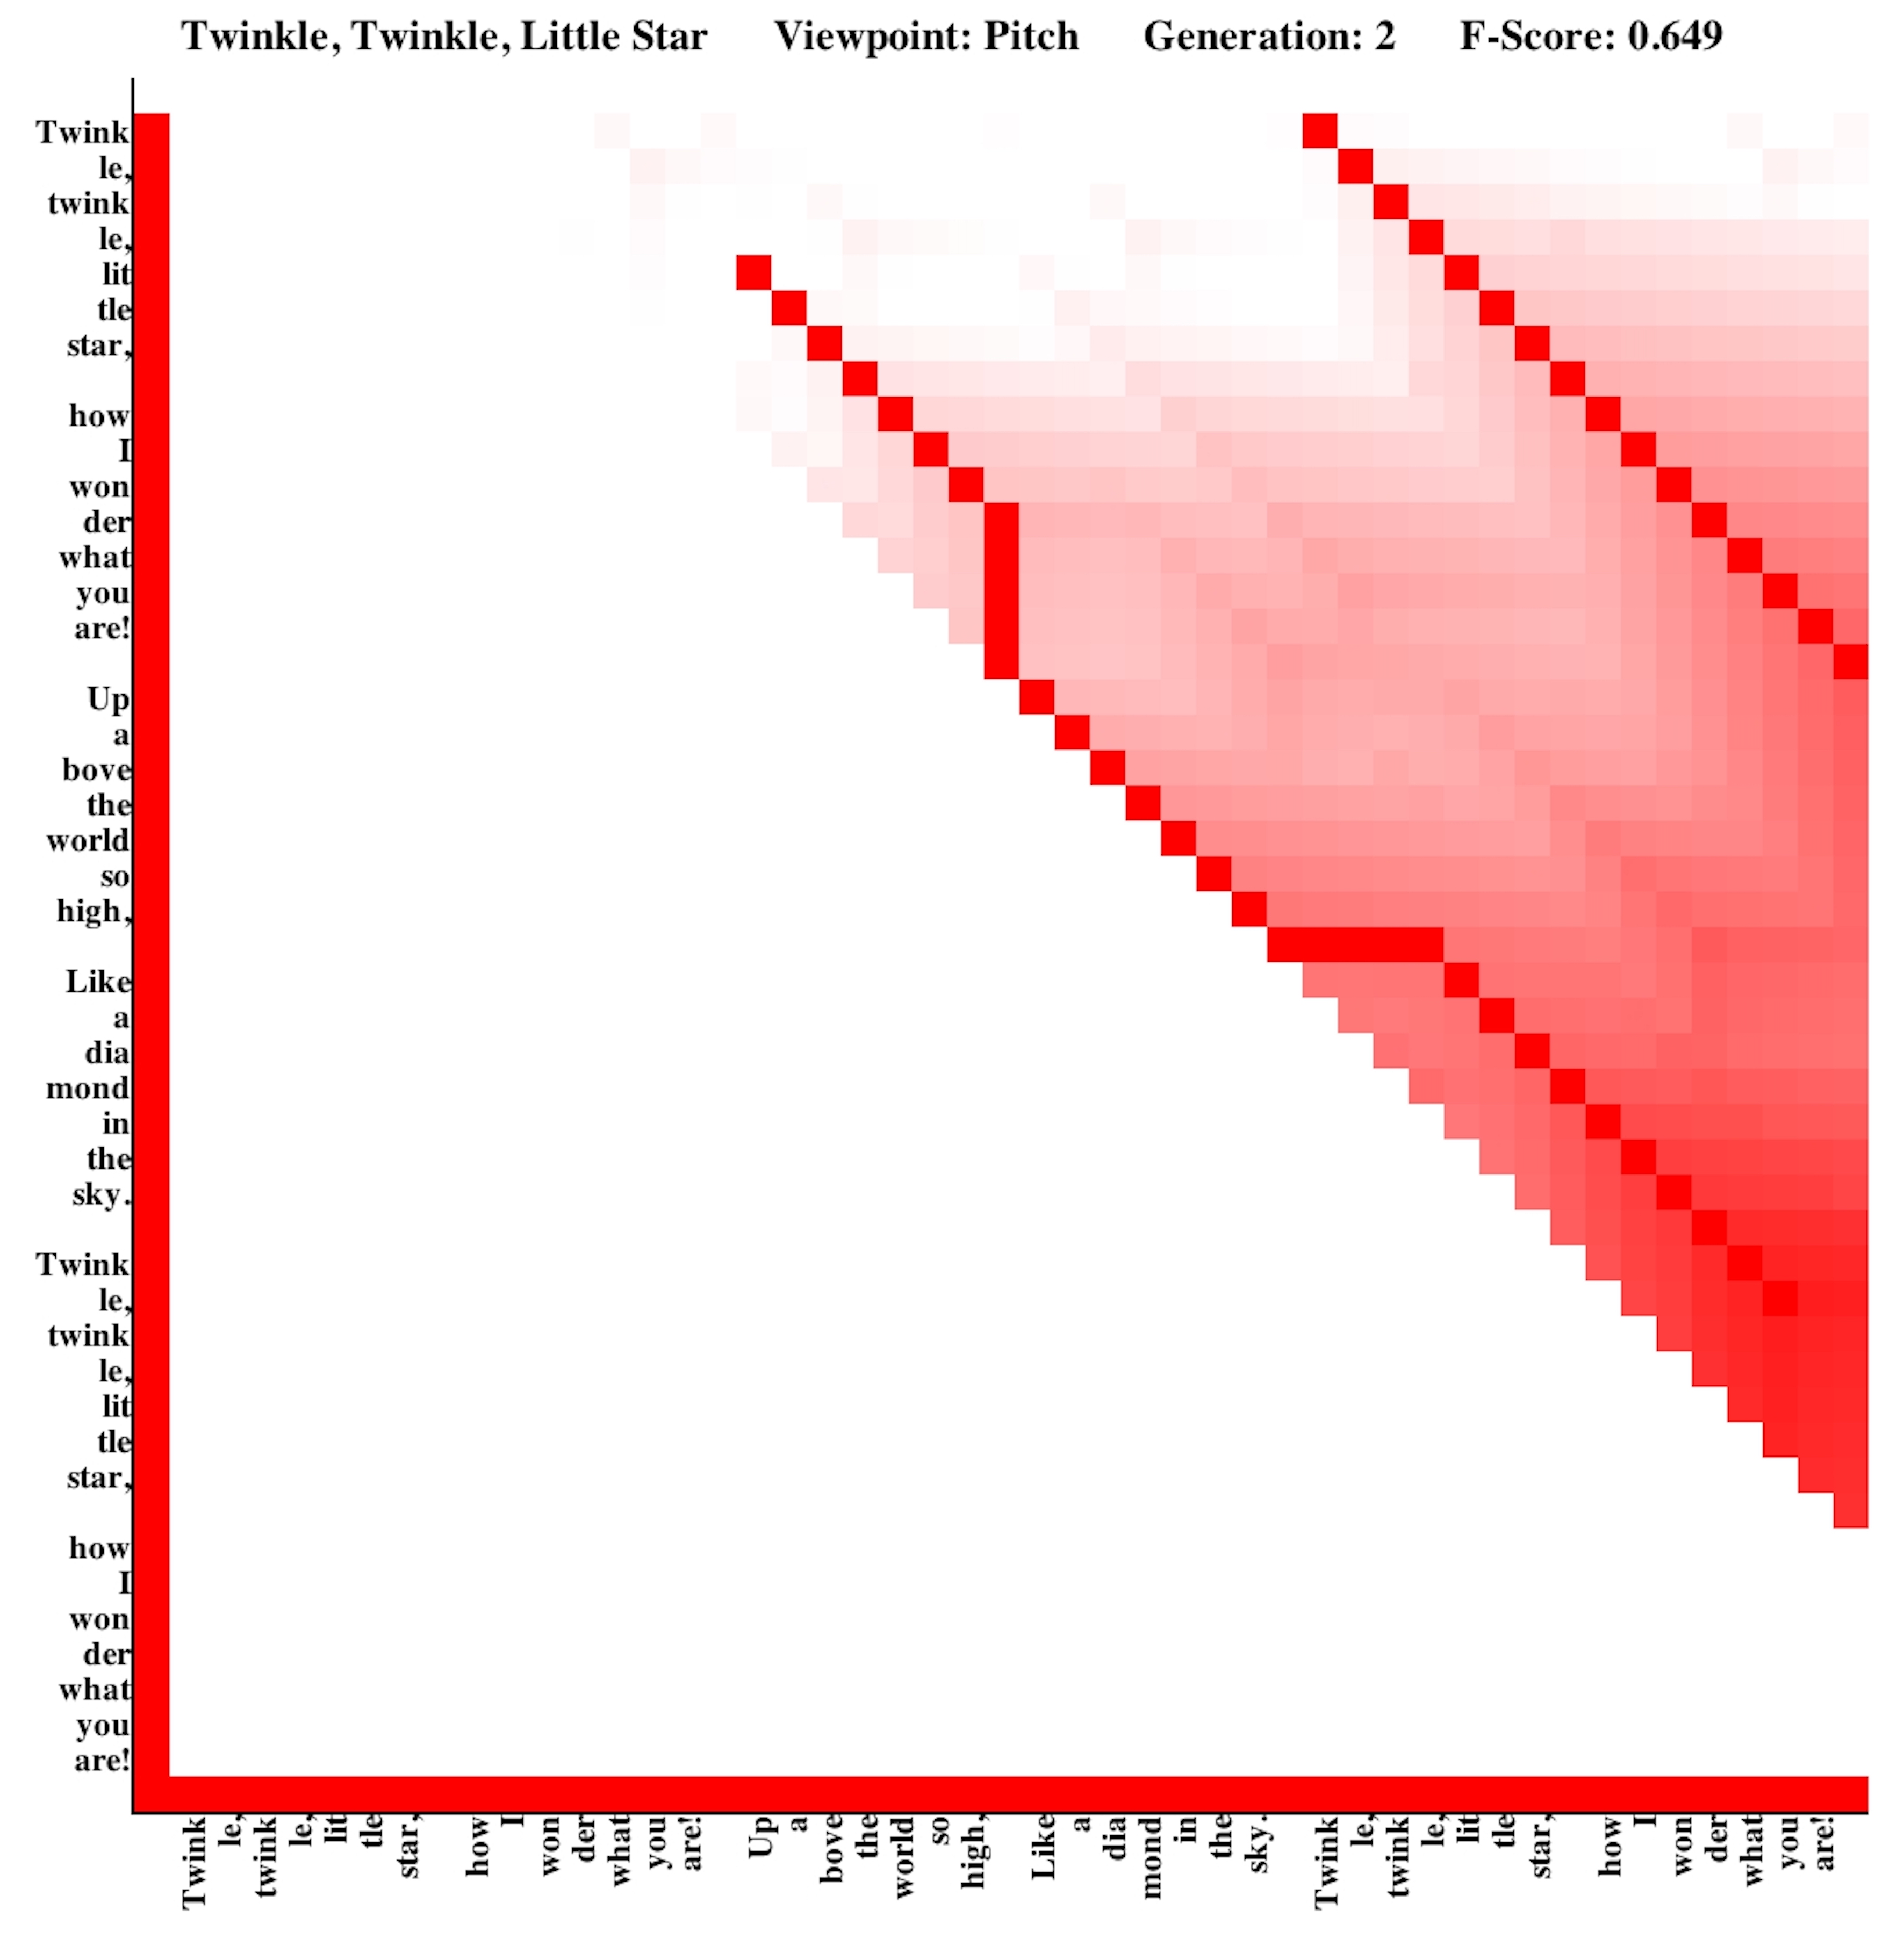
\includegraphics[width=\colwidth]{Twinkle__Twinkle__Little_Star_gen2_id20_pitch} & 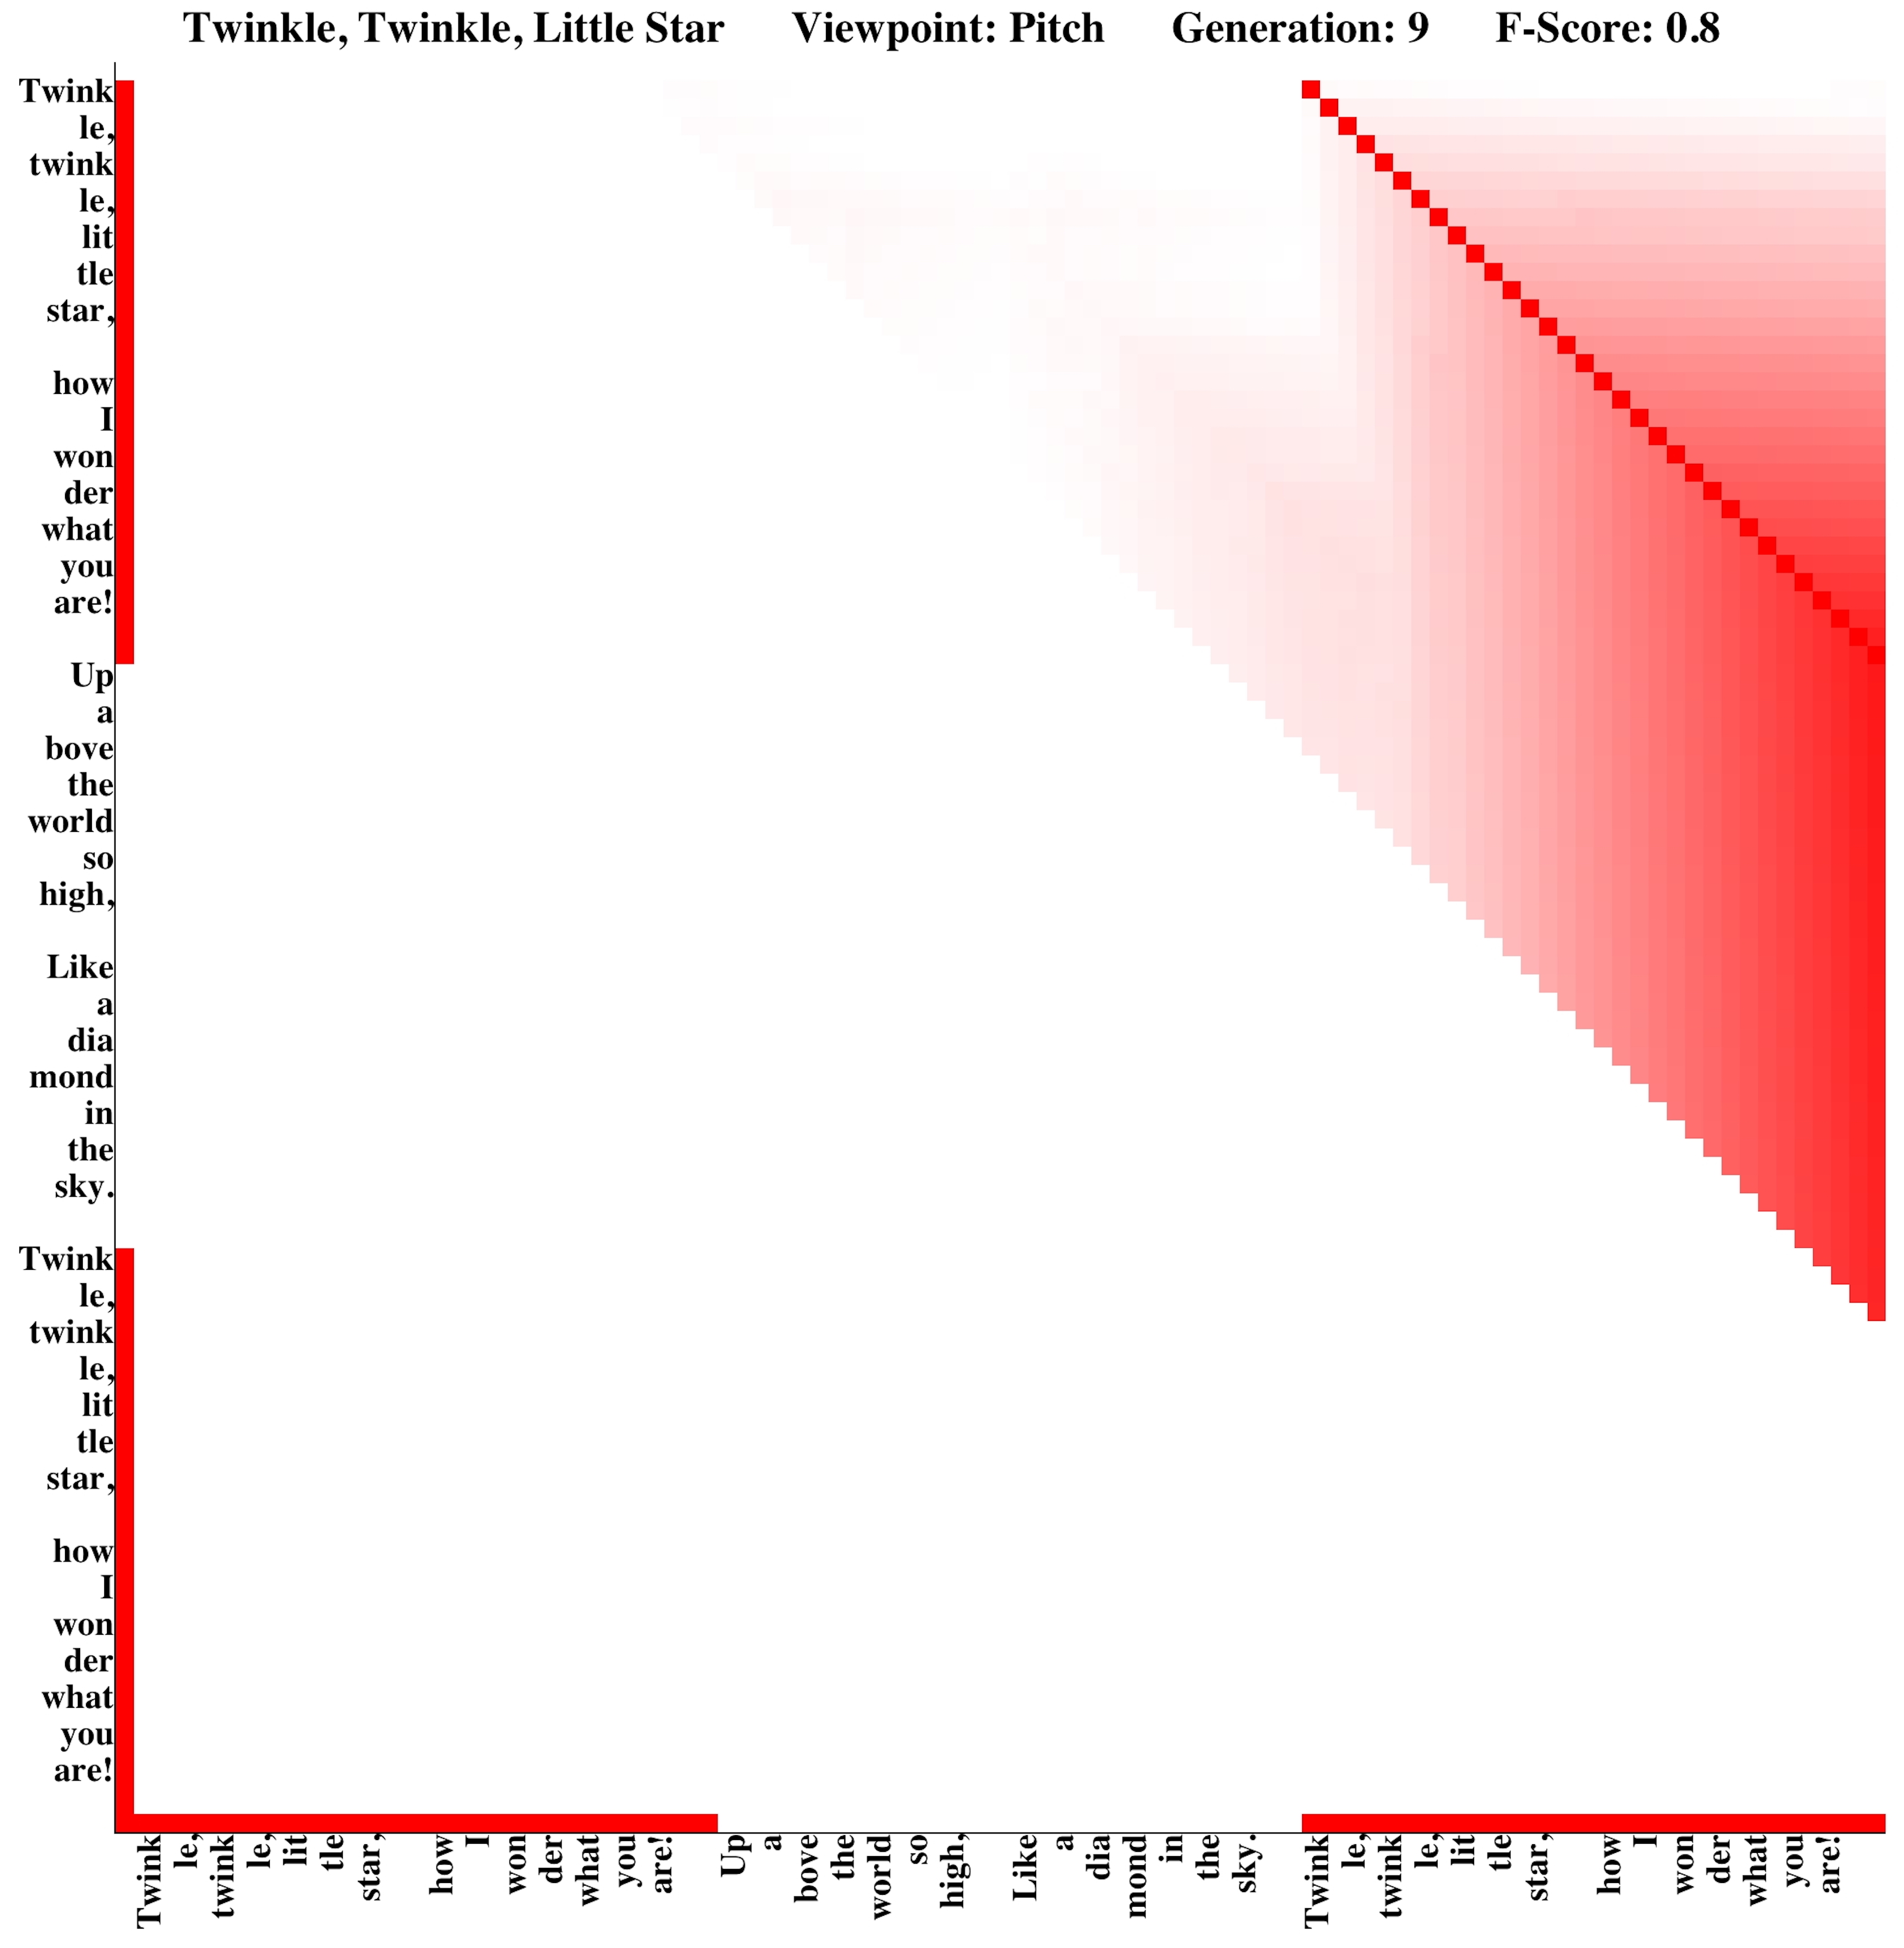
\includegraphics[width=\colwidth]{Twinkle__Twinkle__Little_Star_gen9_id55_pitch} & 
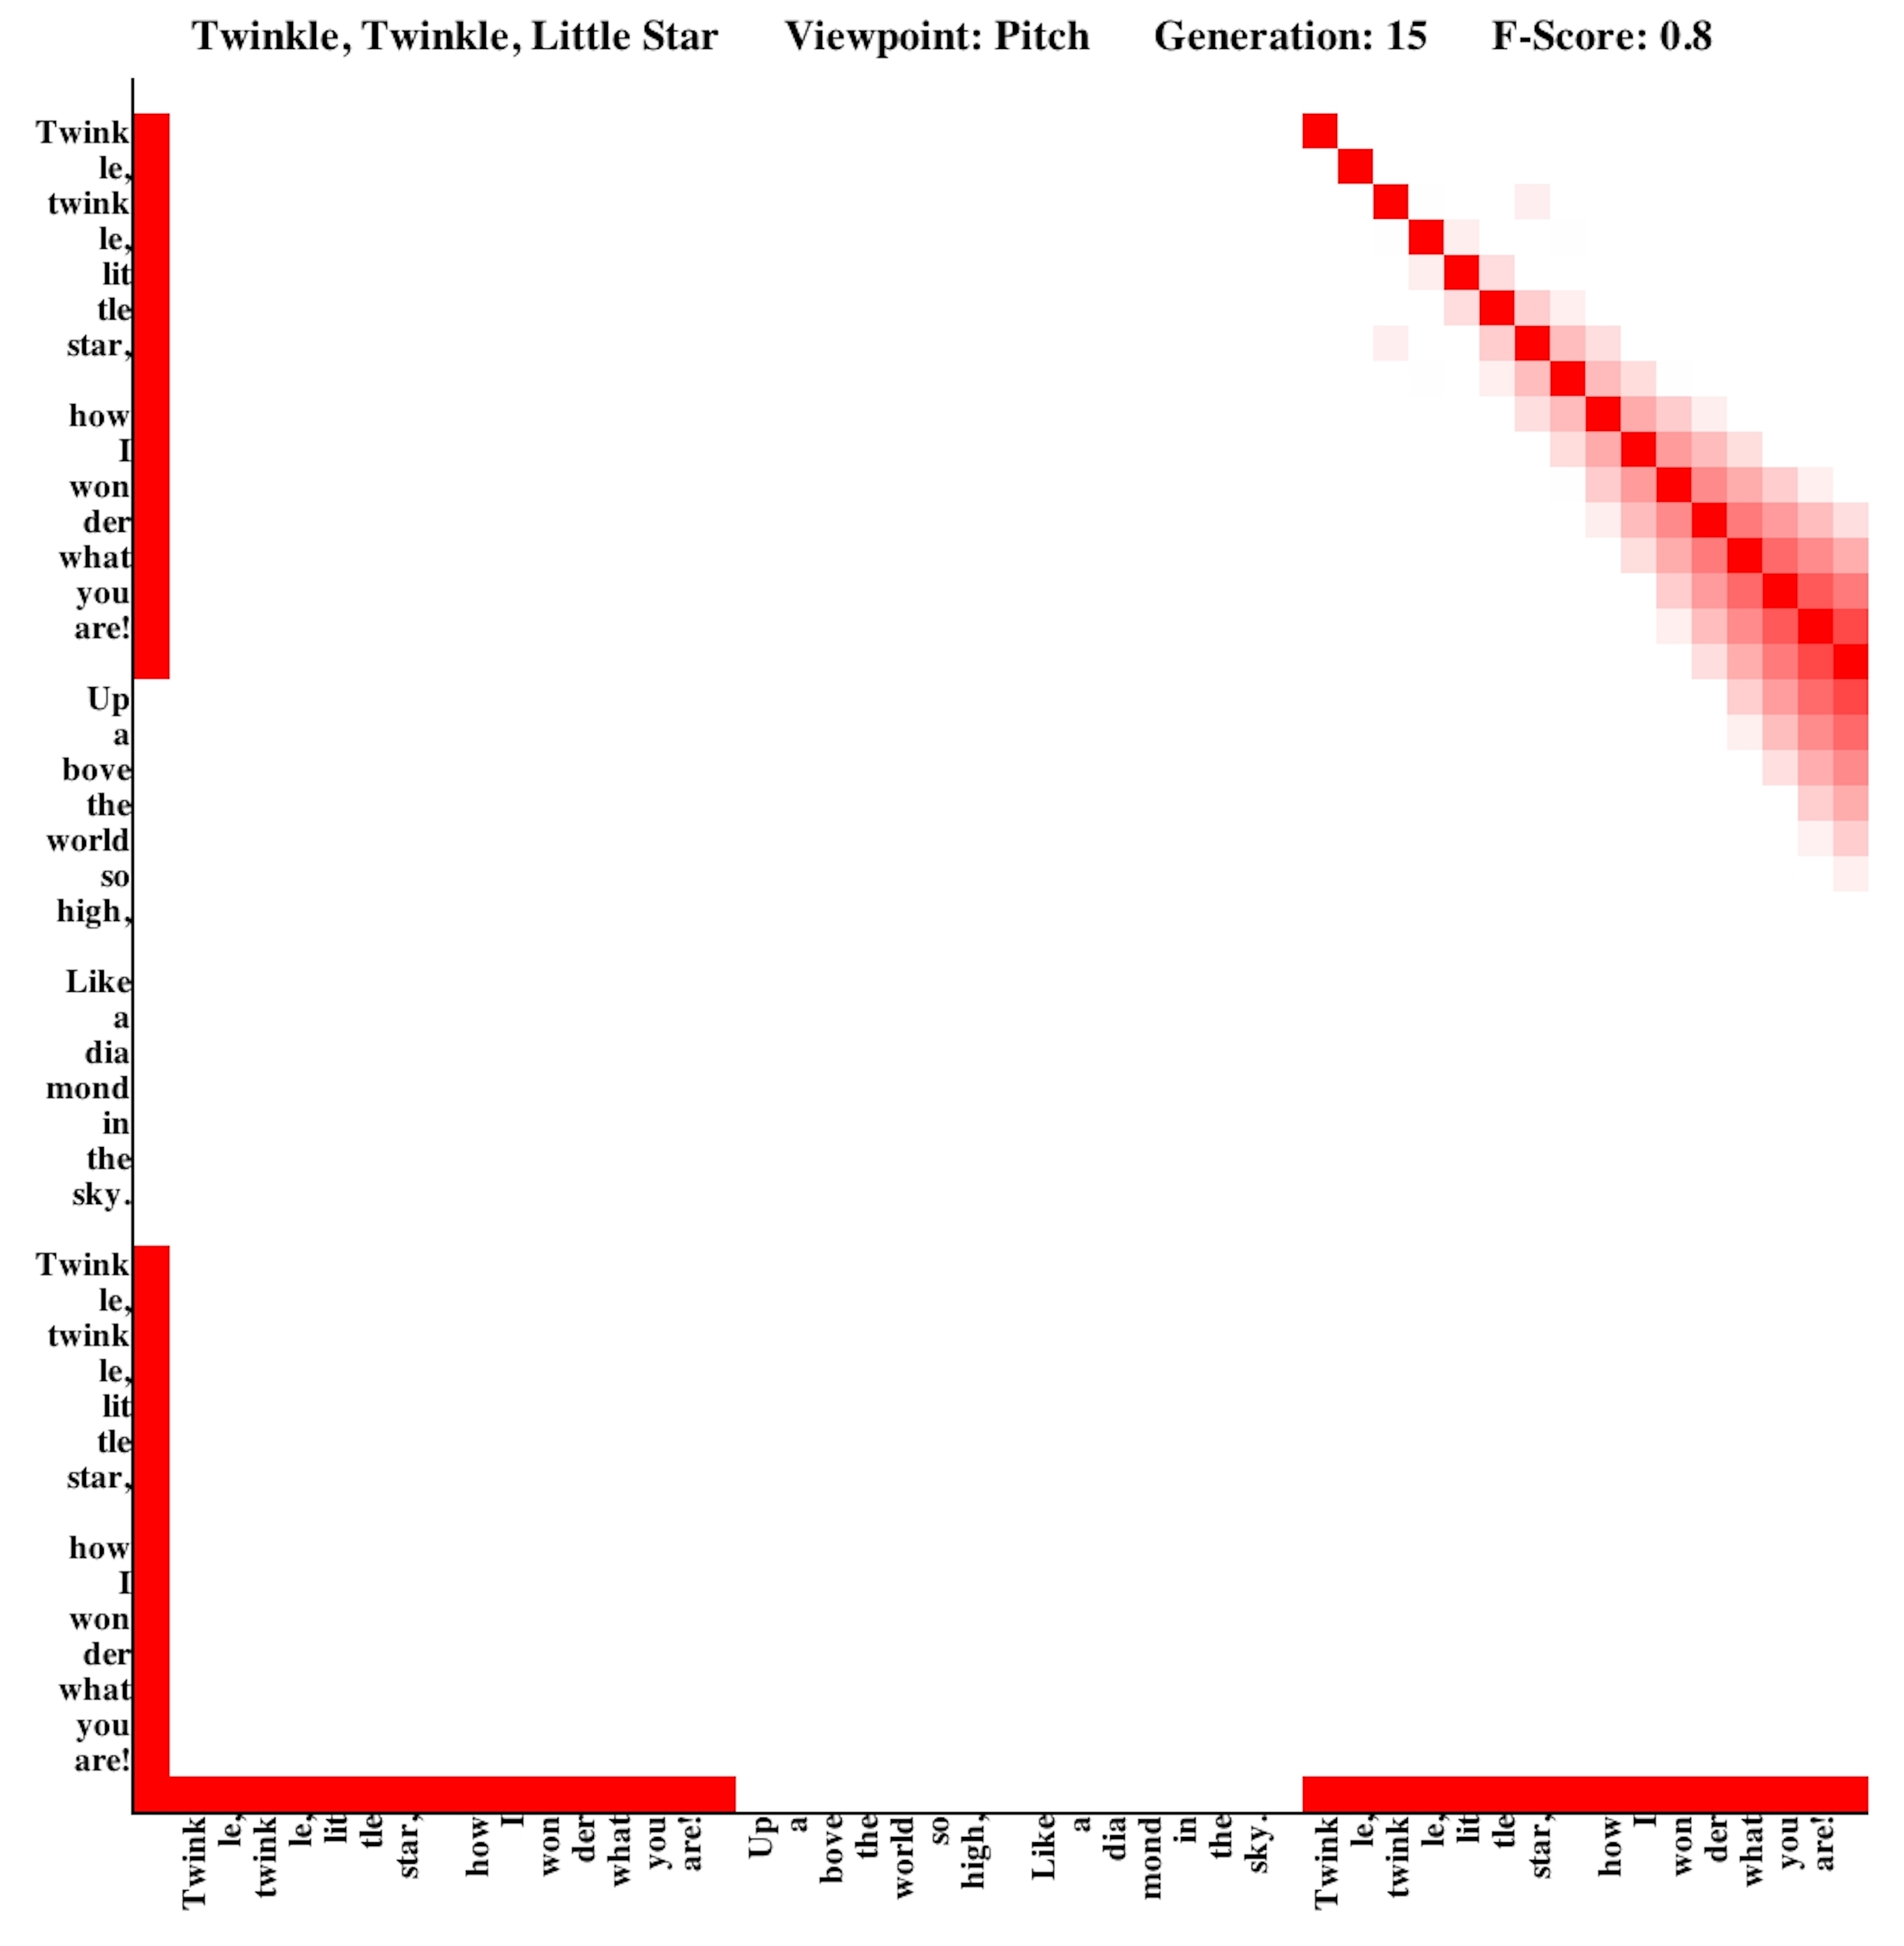
\includegraphics[width=\colwidth]{Twinkle__Twinkle__Little_Star_gen15_id79_pitch} & 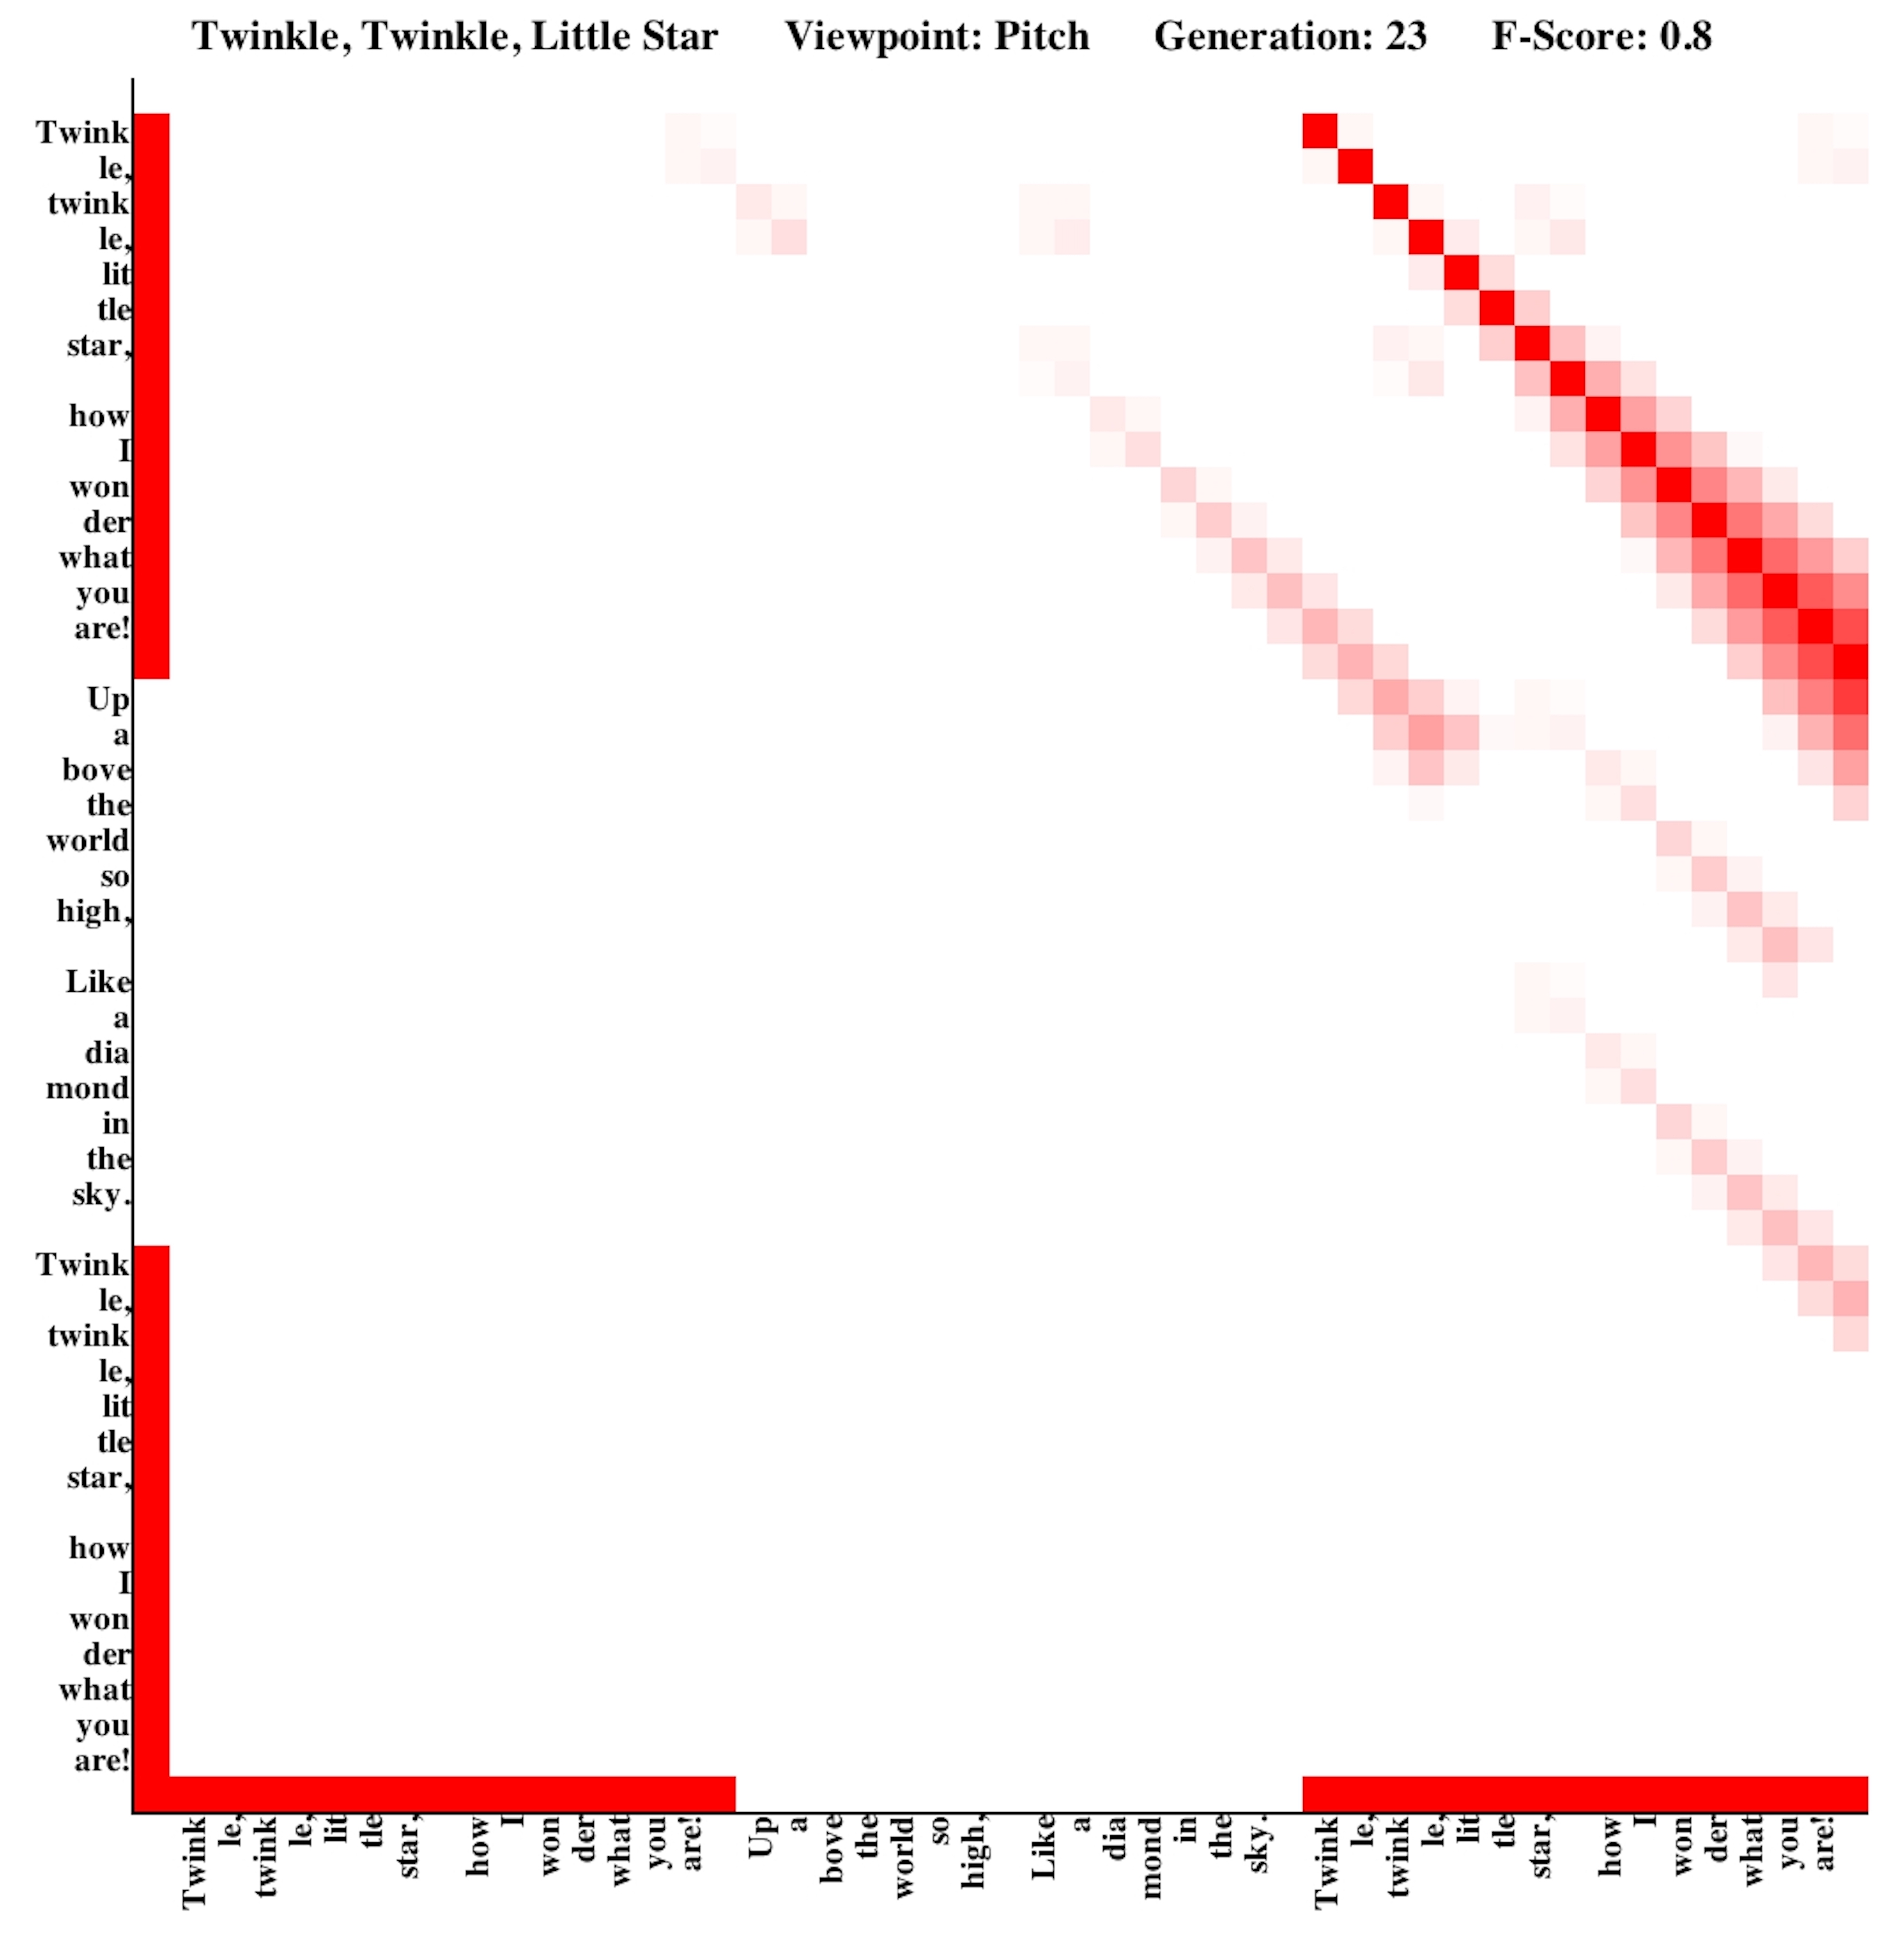
\includegraphics[width=\colwidth]{Twinkle__Twinkle__Little_Star_gen23_id118_pitch} & 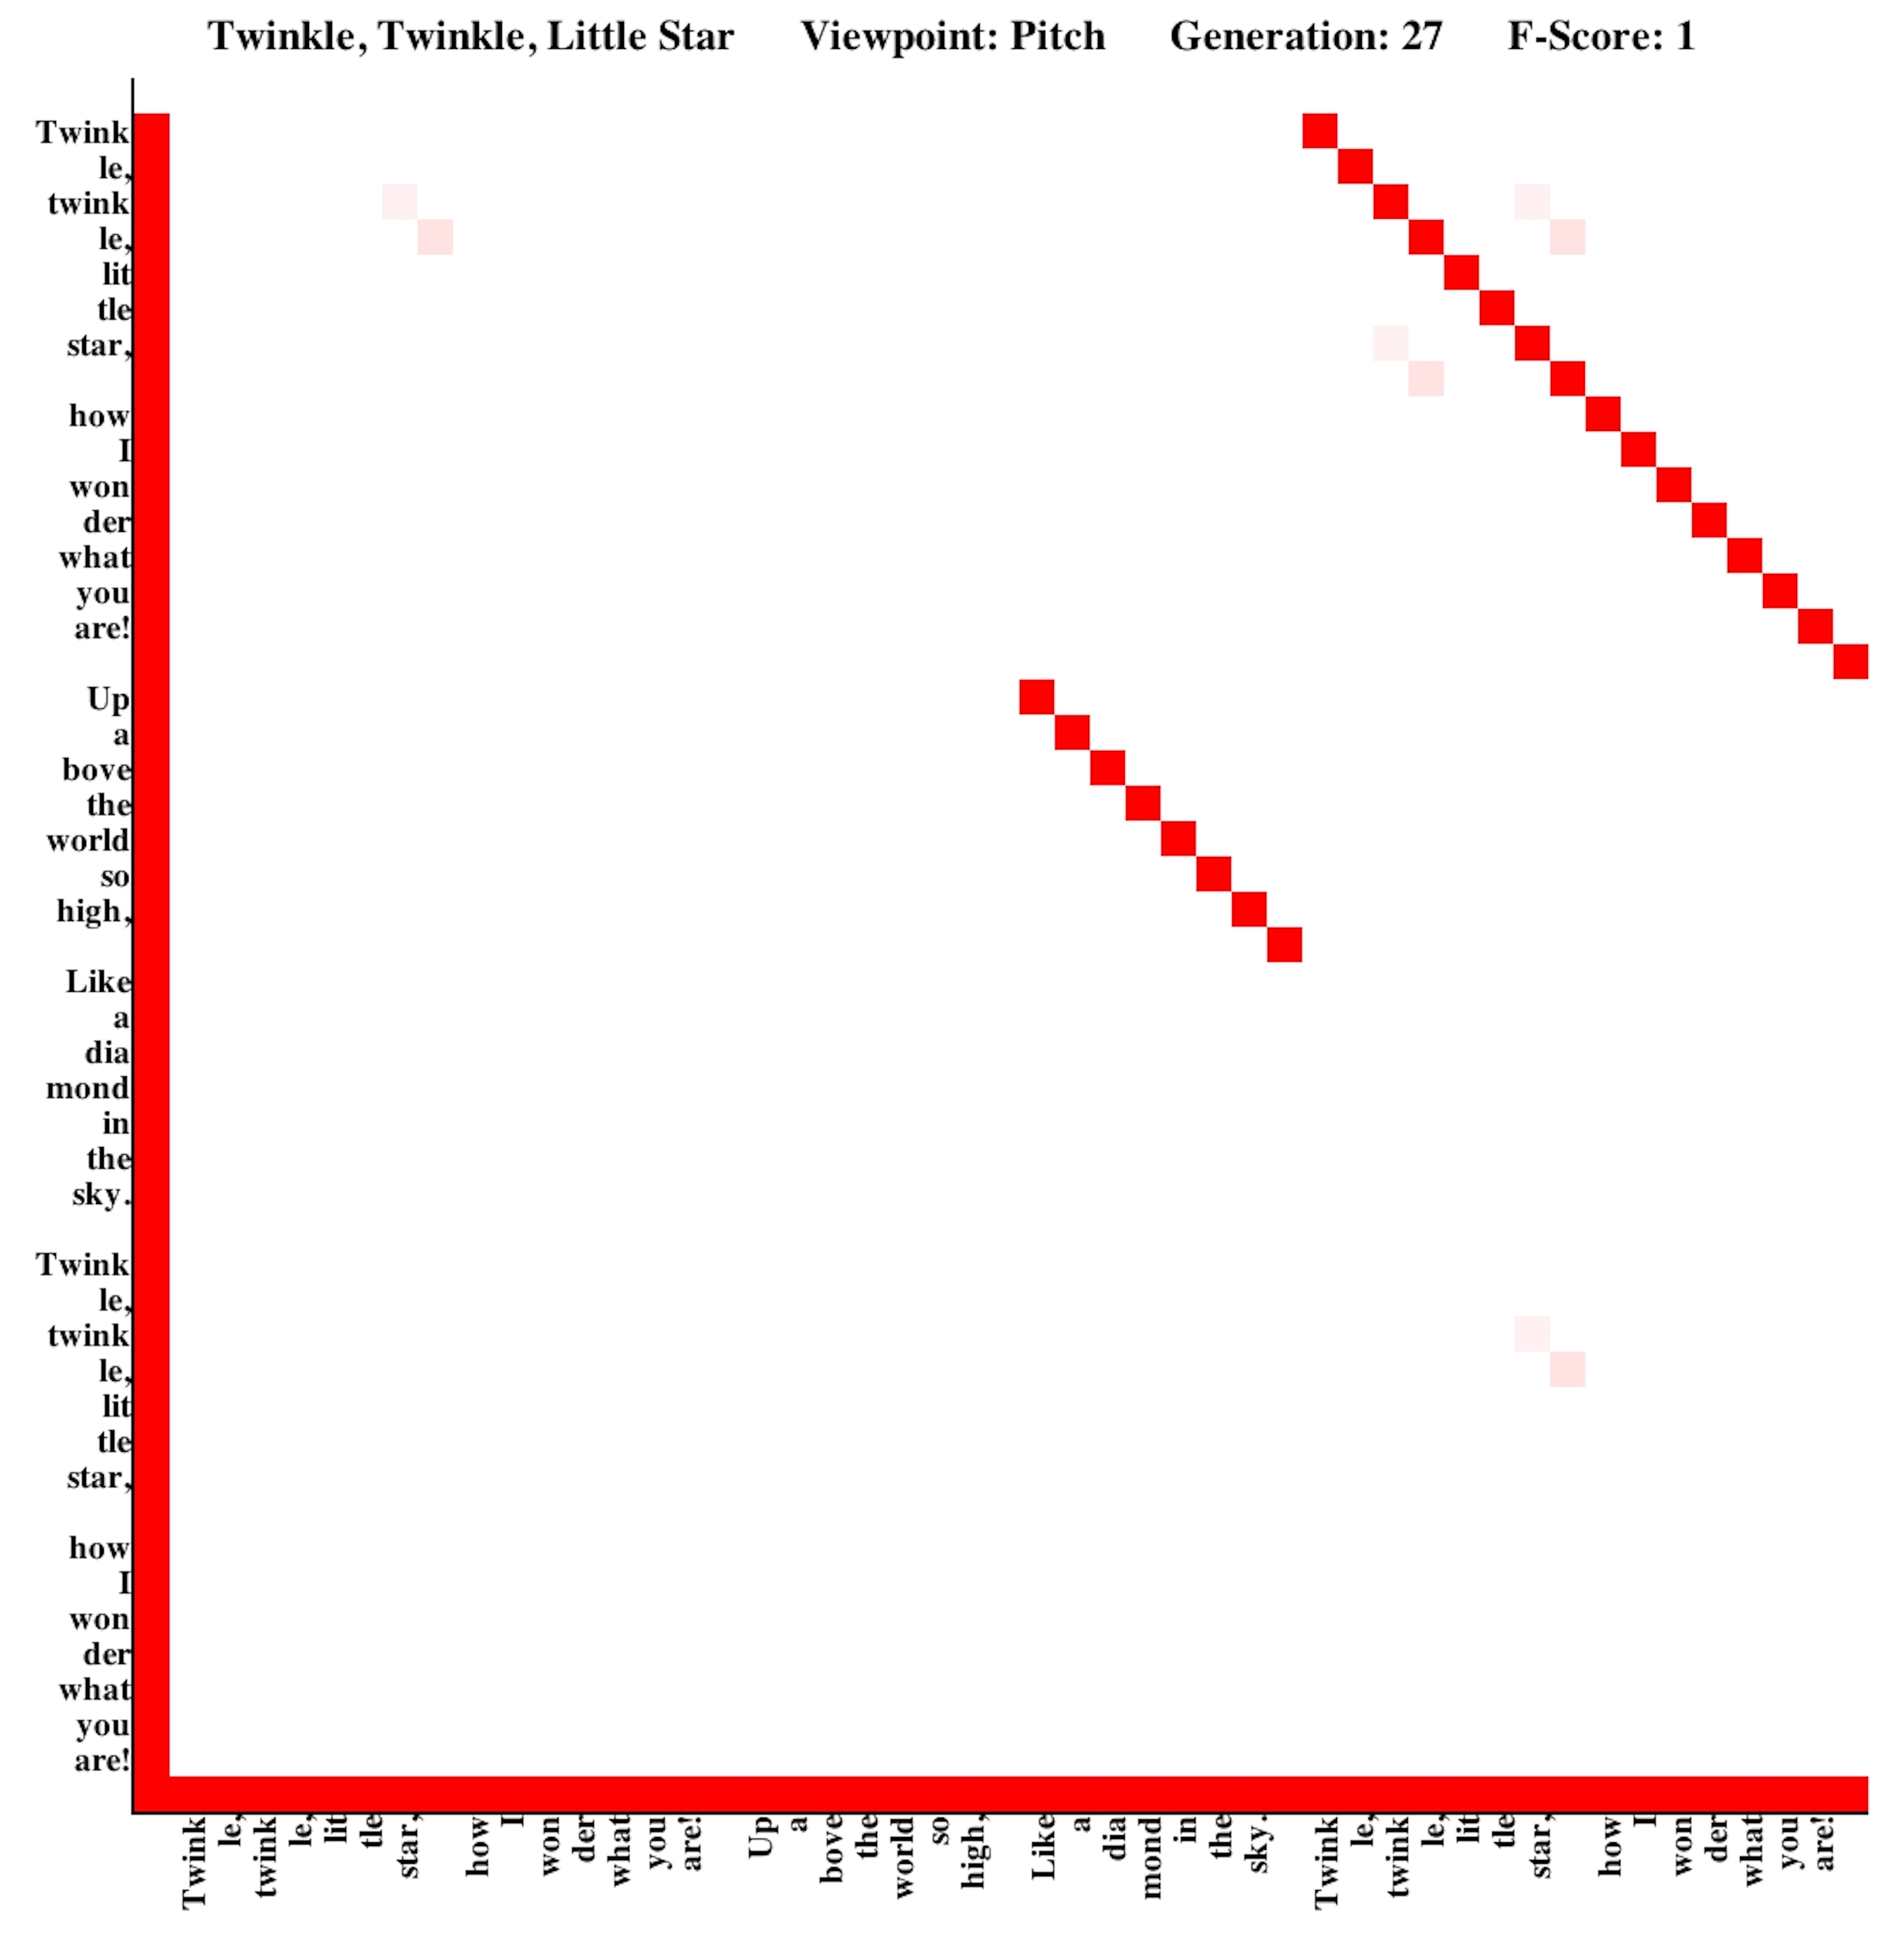
\includegraphics[width=\colwidth]{Twinkle__Twinkle__Little_Star_gen27_id137_pitch} \\
Generation: 1 & Generation: 2  & Generation: 9 & Generation: 15 & Generation: 23 & Generation: 27 \\
$F_{1}=0.34$ & $F_{1}=0.65$ & $F_{1}=0.80$ & $F_{1}=0.80$ & $F_{1}=0.80$ & $F_{1}=1.0$ \\
\end{tabular}
\caption{\label{fig:learning_weights}\textit{Learning weights for the pitch scoring function}. As scoring function weights are adjusted via the GA, different alignments result. We use a multiple Smith-Waterman alignment approach to find all local alignments that result in a score above a threshold $\tau$ (also determined by the GA). As weightings are found that more accurately align (labeled) pitch repetitions, the F-score increases. Shown is the alignment of the song \textit{Twinkle, Twinkle, Little Star}.}
\end{figure*}

Initially we generate a population of 20 unique parameterizations where each parameter is randomly initialized in the range [-3,3] ($\tau$ is randomly initialized in the range [0,20)). For each of 5000 generations of the GA, we generate 10 new parameterizations via 1) \textit{crossover} of two parameterizations randomly selected from the population and then 2) \textit{mutation} where each parameter has a 0.2 probability of adding a random number in the range [-10,10] to its value (with 0.2 probability $\tau$ is multiplied by a factor in the range [0,2)).

\subsubsection{Alignment Fitness Function}
We manually labeled a small subset of the Wikifonia leadsheet dataset with structural repetitions across viewpoints. These labels essentially represent which events we expect to be aligned via our MSW alignment. An event can be aligned with 0, 1, or many other events. We can evaluate a parameterization $\Gamma$ according to the number of event pair alignments that are true positive ($TP$), false positive ($FP$), and true negative ($TN$) when $\Gamma$ is used in our scoring function: %We do this using the F-score:
% (we count events that are accurately aligned to no other events as true positives)
\[ 
F_{1}(\Gamma)=\frac{(1+\beta^2) * TP + 1}{(1+\beta^2) * TP + \beta^2 * FN + FP + 1}
\]
\noindent with $\beta=1.0$ to equally weight recall and precision. We add 1 to the numerator and the denominator to ensure that $F_1$ is defined when no $TP$ are possible (e.g., \textit{Twinkle, Twinkle, Little Star} has no verse). Averaged over all songs in the training data, the F-score represents the fitness of an individual parameterization in our GA. Using this fitness function, we find the optimal parameterization $\Gamma^*_v$ for each viewpoint $v$ %(see Figure~\ref{fig:fscore_v_gens}) %Dan dropped
via its respective alignment scoring function as described below.

Here, F-score should be viewed as a relative rather than absolute measure of performance for several reasons. First, structure is inherently an abstract concept. This means that what should be labeled in our training data as structure is sometimes ambiguous and can be represented along a spectrum of granularity (e.g., hierarchical rhythmic structure). Second, the scoring functions described below are meant primarily to be illustrative. We found that structure learning is sensitive to which features are included and how they are combined. Third, GAs are stochastic by nature, and the (efficiency of) structure learning is sensitive to this stochasticity. %Substituting a neural network with backpropagation for the GA is envisioned as future work, although how that fits into the context of dynamic programming is complex. 
Fourth, we intentionally chose songs with non-trivial structure to see how well this approach would generalize. Thus, even suboptimal F-scores are in many cases reflective of alignments that yield significant structural representation.

%Dan dropped
%Dan dropped
%\begin{figure}
%	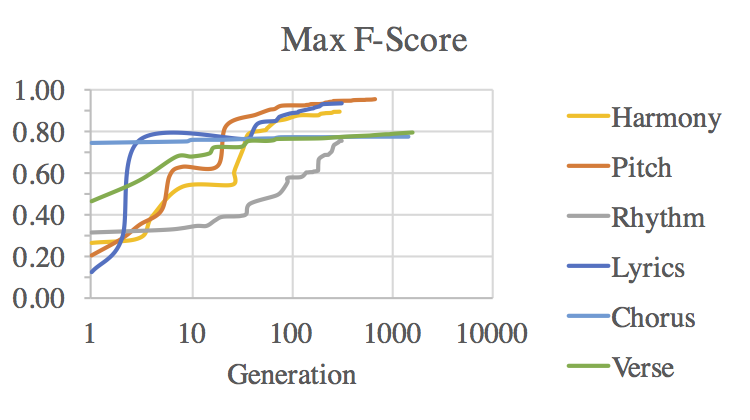
\includegraphics[width=\linewidth]{Max_f_score}
%    \caption{\label{fig:fscore_v_gens}\textit{Learning weights for multiple viewpoints}. Parameterizations for viewpoints were trained via GA for 5000 generations. The graph shows the F-score for the best individual parameterization for each generation (while stil increasing). Rhythm proved more difficult than other primitive viewpoints, likely because rhythm in lyrical music is more readily overlooked when identifying structure than variation in other viewpoints, making it more difficult to distinguish structural patterns from non-structural similarities. The irregular increases in F-score are indicative of the stochasticity of the GA. Because the Chorus and Verse alignment functions use pretrained primitive viewpoint alignment functions,  most of the difficult learning for these combinatorial features is done \textit{a priori}, thus requiring fewer generations to find optimal parameterizations.}
%\end{figure}

\subsubsection{Alignment Scoring Functions}

%The intractable range of musical events necessitates defining a dynamic scoring function, meaning a function that does not rely on lookup tables, to determine the similarity of two events. This function should assign a high score to pairs of events that are similar (per viewpoint) and a low score to pairs that are dissimilar.%Dan dropped

%In our case w
We define six different scoring functions: one scoring function for each of the primitive viewpoints of harmony, pitch, rhythm, and lyrics, and one scoring function for each of the derived viewpoints representing chorus and verse structures. Each scoring function scores the similarity of two musical events using a unique subset of event features that are indicative of self-similarity in that viewpoint.

Since structural repetitions in music tend to preserve meter, all viewpoint alignment functions are designed to consider the offset within the measure of the two events being aligned. For events $e_1$ an $e_2$ we define a beat matching subfunction $M_B(e_1,e_2)$ for this offset alignment as
\[
  M_B(e_1,e_2) =
  \begin{cases}
	\iota_B & \text{if } b_1 = b_2 \\
	\Delta_B + \delta_B * |b_1 - b_2| & \text{if } b_1 \neq b_2 
  \end{cases}
\]
\noindent where $b_i=beat(e_i)$ and $\iota_B$, $\Delta_B$, and $\delta_B$ are weights determined for each viewpoint by the GA.

\subsubsection{Harmony}

A harmony $harmony(e_i)$ represents a set of pitches which we denote $notes(harmony(e_i)) = \{p_1,\cdots,p_n\}$ where each pitch $p_i$ is a MIDI note value modulo 12 to normalize values to a common octave. Using the shorthand $N_i = notes(harmony(e_i))$ we define a harmonic scoring function $S_H(e_1,e_2)$ as follows:
\[
  S_H(e_1,e_2) = I_H(e_1,e_2) + O_H(e_1,e_2) + M_B(e_1,e_2)
\]
\noindent with the identity subfunction $I_H(e_1,e_2)$ computed as
\[ I_H(e_1,e_2) = 
  \begin{cases}
  	\iota_H & \text{if } N_1 = N_2 \\
    \Delta_H + \delta_H/ Z(N_1,N_2) & \text{if } N_1 \neq N_2
  \end{cases}
\]
\noindent where the set similarity function $Z(N_1,N_2)$ is defined as
\[
Z(N_1,N_2) = (2*|N_1\cap N_2|/(|N_1|+|N_2|))
\]
\noindent Letting $o_i = is\_harmony\_onset(e_i)$,
\[ O_H(e_1,e_2) = 
  \begin{cases}
  	\Omega_H & \text{if } o_1 \land o_2 \\
    \omega_H & \text{if } o_1 \lor o_2 \\
    \gamma_H & \text{otherwise}
  \end{cases}
\]
\noindent In this manner, $\iota_H$, $\Delta_H$, $\delta_H$, $\Omega_H$, $\omega_H$, and $\gamma_H$ represent weights to be learned by the GA.

\subsubsection{Pitch}

Letting $r_i = is\_rest(e_i)$ and $p_i = pitch(e_i)$, we compute the pitch score $S_P(e_1,e_2)$ of events $e_1$ and $e_2$ as 
\[
S_P(e_1,e_2) =
  \begin{cases}
	R & \text{if } r_1 \land r_2 \\
	\rho & \text{if } r_1 \lor r_2 \\ 
    \gamma_R + M_P(e_1,e_2) & \text{otherwise}
  \end{cases}
\]
\noindent with $M_P(e_1,e_2)$ representing the pitch matching subfunction for scoring two events:
\[ M_P(e_1,e_2) = I_P(e_1,e_2) + O_P(e_1,e_2) + M_B(e_1,e_2) \]
\noindent with
\[ I_P(e_1,e_2) = 
  \begin{cases}
  	\iota_P & \text{if } p_1 = p_2 \\
    \Delta_P + \delta_P * |p_1-p_2| & \text{if } p_1 \neq p_2
  \end{cases}
\]
\noindent letting $o_i = is\_pitch\_onset(e_i)$,
\[ O_P(e_1,e_2) = 
  \begin{cases}
  	\Omega_P & \text{if } o_1 \land o_2 \\
    \omega_P & \text{if } o_1 \lor o_2 \\
    \gamma_P & \text{otherwise}
  \end{cases}
\]
\noindent Again $R$, $\rho$, $\gamma_R$, $\iota_P$, $\Delta_P$, $\delta_P$, $\Omega_P$, $\omega_P$, and $\gamma_P$ represent weights to be learned by the GA.

\subsubsection{Rhythm}

Letting $r_i = is\_rest(e_i)$ and $d_i = duration(e_i)$, we compute the melodic rhythm score $S_R(e_1,e_2)$ as 
\[
S_R(e_1,e_2) = M_R(e_1,e_2) * (I_D(e_1,e_2) + O_P(e_1,e_2) + M_B(e_1,e_2))
\]
\noindent with $M_R(e_1,e_2)$ representing the rest matching subfunction for scoring two events:
\[ M_R(e_1,e_2) = 
  \begin{cases}
  	R & \text{if } r_1 \land r_2 \\
    \rho & \text{if } r_1 \lor r_2 \\
    \gamma_R & \text{otherwise}
  \end{cases}
\]
\noindent with
\[ I_D(e_1,e_2) = 
  \begin{cases}
  	\iota_D & \text{if } d_1 = d_2 \\
    \Delta_D + \delta_D * |d_1-d_2| & \text{if } d_1 \neq d_2
  \end{cases}
\]
\noindent $R$, $\rho$, $\gamma_R$, $\iota_D$, $\Delta_D$, and $\delta_D$ are weights learned by the GA.

%Dan dropped
%\begin{figure*}[ht]
%\centering
%\begin{tabular}{rl}
%\textbf{Harmony} & \begin{tabular}{@{}l@{}}\textit{Genetic Representation}: $\Gamma_H = (G_o,G_e,\tau, \iota_B, \Delta_B, \delta_B, \iota_H, \Delta_H, \delta_H, \Omega_H, \omega_H, \gamma_H)$ \\ \textit{Best Solution}: $\Gamma^*_H$ = (-4, -18, 16.89, 3.23, 3.42, -0.24, 0.39, 1.32, -16.99, -0.97, -10.76, -3.23)\end{tabular} \\  \vspace{.06cm}
%\textbf{Pitch} & \begin{tabular}{@{}l@{}}\textit{Genetic Representation}: $\Gamma_P = (G_o,G_e,\tau, \iota_B, \Delta_B, \delta_B, R, \rho, \gamma_R, \iota_P, \Delta_P, \delta_P, \Omega_P, \omega_P, \gamma_P)$ \\ \textit{Best Solution}: $\Gamma^*_P$ = (-18, -11, 27.64, 2, -11.76, -25.79, 3.43, -1.44, -6.88, 4.78, 8.46, -3.53, 3, 0.44, 0.97)\end{tabular} \\  \vspace{.06cm}
%\textbf{Rhythm} & \begin{tabular}{@{}l@{}}\textit{Genetic Representation}: $\Gamma_R = (G_o,G_e,\tau, \iota_B, \Delta_B, \delta_B, R, \rho, \gamma_R, \iota_D, \Delta_D, \delta_D, \Omega_P, \omega_P, \gamma_P)$ \\ \textit{Best Solution}: $\Gamma^*_R$ = (-16, -2, 5.84, -5.49, -3.15, -27.99, 0.3, 0.28, 1.38, 10.53, 14.82, -10.9, -4.86, -6.61, -4.9)\end{tabular} \\  \vspace{.06cm}
%\textbf{Lyric} & \begin{tabular}{@{}l@{}}\textit{Genetic Representation}: $\Gamma_L = (G_o,G_e,\tau, \iota_B, \Delta_B, \delta_B, R, \rho, N, \nu, \iota_L, \Delta_L, \Omega_L, \omega_L, \gamma_L)$ \\ \textit{Best Solution}: $\Gamma^*_L$ = (-5, -13, 24.1, -2.24, -11.15, -28.18, -4.56, -9.26, 3.11, -10.39, -1.72, -10.99, 7.38, 5.06, 4.83)\end{tabular} \\ \vspace{.06cm}
%\textbf{Chorus} & \begin{tabular}{@{}l@{}}\textit{Genetic Representation}: $\Gamma_C = (G_o,G_e,\tau, \iota_B, \Delta_B, \delta_B, w_H, w_P, w_R, w_L)$ \\ \textit{Best Solution}: $\Gamma^*_C$ = (-32, -20, 137.92, 9.05, -11.51, 16.18, 0.43, 3, 0, 4.45)\end{tabular} \\ \vspace{.06cm}
%\textbf{Verse} & \begin{tabular}{@{}l@{}}\textit{Genetic Representation}: $\Gamma_V = (G_o,G_e,\tau, \iota_B, \Delta_B, \delta_B, w_H, w_P, w_R, w_L)$ \\ \textit{Best Solution}: $\Gamma^*_V$ = (-7, -17, 313.41, -3.18, 4.18, -3.79, 3, 3.49, 0.07, 1.13)\end{tabular}
%\end{tabular}
%\caption{\label{fig:final_weights}\textit{Best viewpoint parameterization $\Gamma^*_v$ for each viewpoint $v$ from the GA after 5000 generations}.}
%\end{figure*}

\subsubsection{Lyrics}

Intuitively structural patterns in lyrics are a product of word sequences that repeat. This happens, for example, in choruses or taglines. It does happen on occasion that different iterations of the chorus contain added words or phrases for which some flexibility is needed. Thus we design the lyric scoring function in order to allow the GA to learn appropriate weights for pairs of notes in which one or both notes are either rests or non-lyrical. We also design the lyric scoring function to learn weights that favor the alignment of lyric onsets.

For two events $e_1$ and $e_2$, we compute the lyric score $S_L(e_1,e_2)$. Letting $r_i = is\_rest(e_i)$ and $l_i = lyric(e_i)$,
\[
  S_L(e_1,e_2) =
  \begin{cases}
	R & \text{if } r_1 \land r_2 \\
	\rho & \text{if } r_1 \lor r_2 \\ 
    N & \text{if } l_1 = \varnothing \land l_2 = \varnothing\\
    \nu & \text{if } l_1 = \varnothing \lor l_2 = \varnothing \\
    M_L(e_1,e_2) & \text{otherwise}
  \end{cases}
\]
\noindent with $M_L(e_1,e_2)$ representing the lyric matching subfunction for scoring two events with non-empty lyrics:
\[ M_L(e_1,e_2) = I_L(e_1,e_2) + O_L(e_1,e_2) + M_B(e_1,e_2) \]
\noindent with
\[ I_L(e_1,e_2) = 
  \begin{cases}
  	\iota_L & \text{if } l_1 = l_2 \\
    \Delta_L & \text{if } l_1 \neq l_2
  \end{cases}
\]
\noindent Letting $o_i = is\_lyric\_onset(E_i)$,
\[ O_L(e_1,e_2) = 
  \begin{cases}
  	\Omega_L & \text{if } o_1 \land o_2 \\
    \omega_L & \text{if } o_1 \lor o_2 \\
    \gamma_L & \text{otherwise}
  \end{cases}
\]
\noindent $R$, $\rho$, $N$, $\nu$, $\iota_L$, $\Delta_L$, $\Omega_L$, $\omega_L$ and $\gamma_L$ are learned by the GA.

\subsubsection{Chorus and Verse}

Having defined scoring functions for primitive viewpoint alignments, we can now define compound scoring functions for more abstract feature alignment. Consider, for example, that a chorus is generally defined as a musical subsequence in which harmony, pitch, rhythm, and lyrics repeat. A verse is generally defined as a musical subsequence in which harmony, pitch, and rhythm repeat, and lyrics do not repeat. Given that both of these abstract features consider the same set of primitive features, we define a single compound scoring function that can be used (with different parameterizations) to learn structure for both. 

For two events $e_1$ and $e_2$, we compute a compound alignment score $S_C(e_1,e_2)$ as
\[
S_C(e_1,e_2) = w_H * S_H(e_1,e_2) + w_P * S_P(e_1,e_2) + w_R * S_R(e_1,e_2) + w_L * S_L(e_1,e_2)
\]
\noindent with $w_H$, $w_P$, $w_R$, and $w_L$ representing the weights (to be determined by the GA) of the viewpoints harmony, pitch, rhythm, and lyric respectively, and each of the viewpoint-specific scoring functions as defined above. In learning these abstract features we use optimal parameterizations $\Gamma^*_H$, $\Gamma^*_P$, $\Gamma^*_R$, and $\Gamma^*_L$ for the subscoring functions as learned on the respective viewpoint-specific alignment tasks% (see Figure~\ref{fig:final_weights}) %Dan dropped
. For learning verse structure, the values of $\iota_L$ and $\Delta_L$ in $\Gamma^*_L$ are swapped because $\Gamma^*_L$ is trained to find where lyrics are similar and verses require lyrics which are different (in similar positions). General alignment parameters $G_o$, $G_e$, and $\tau$ for subscoring functions are ignored.

\begin{figure*}[t!]
\centering
\newcommand{\colwidth}{1in}
\setlength\tabcolsep{1.5pt} % default value: 6pt
\newcolumntype{C}{ >{\centering\arraybackslash} m{.7in} }
\newcolumntype{D}{ >{\centering\arraybackslash} m{\colwidth} }
\begin{tabular}{CDDDDDD}
 & \textbf{Harmony} & \textbf{Pitch} & \textbf{Rhythm} & \textbf{Lyric} & \textbf{Chorus} & \textbf{Verse} \\
  & $F_{1}=0.90$ & $F_{1}=0.95$ & $F_{1}=0.78$ & $F_{1}=0.94$ & $F_{1}=0.78$ & $F_{1}=0.80$ \\
\textbf{Twinkle, Twinkle Little Star} $F_{1}=0.99$ & 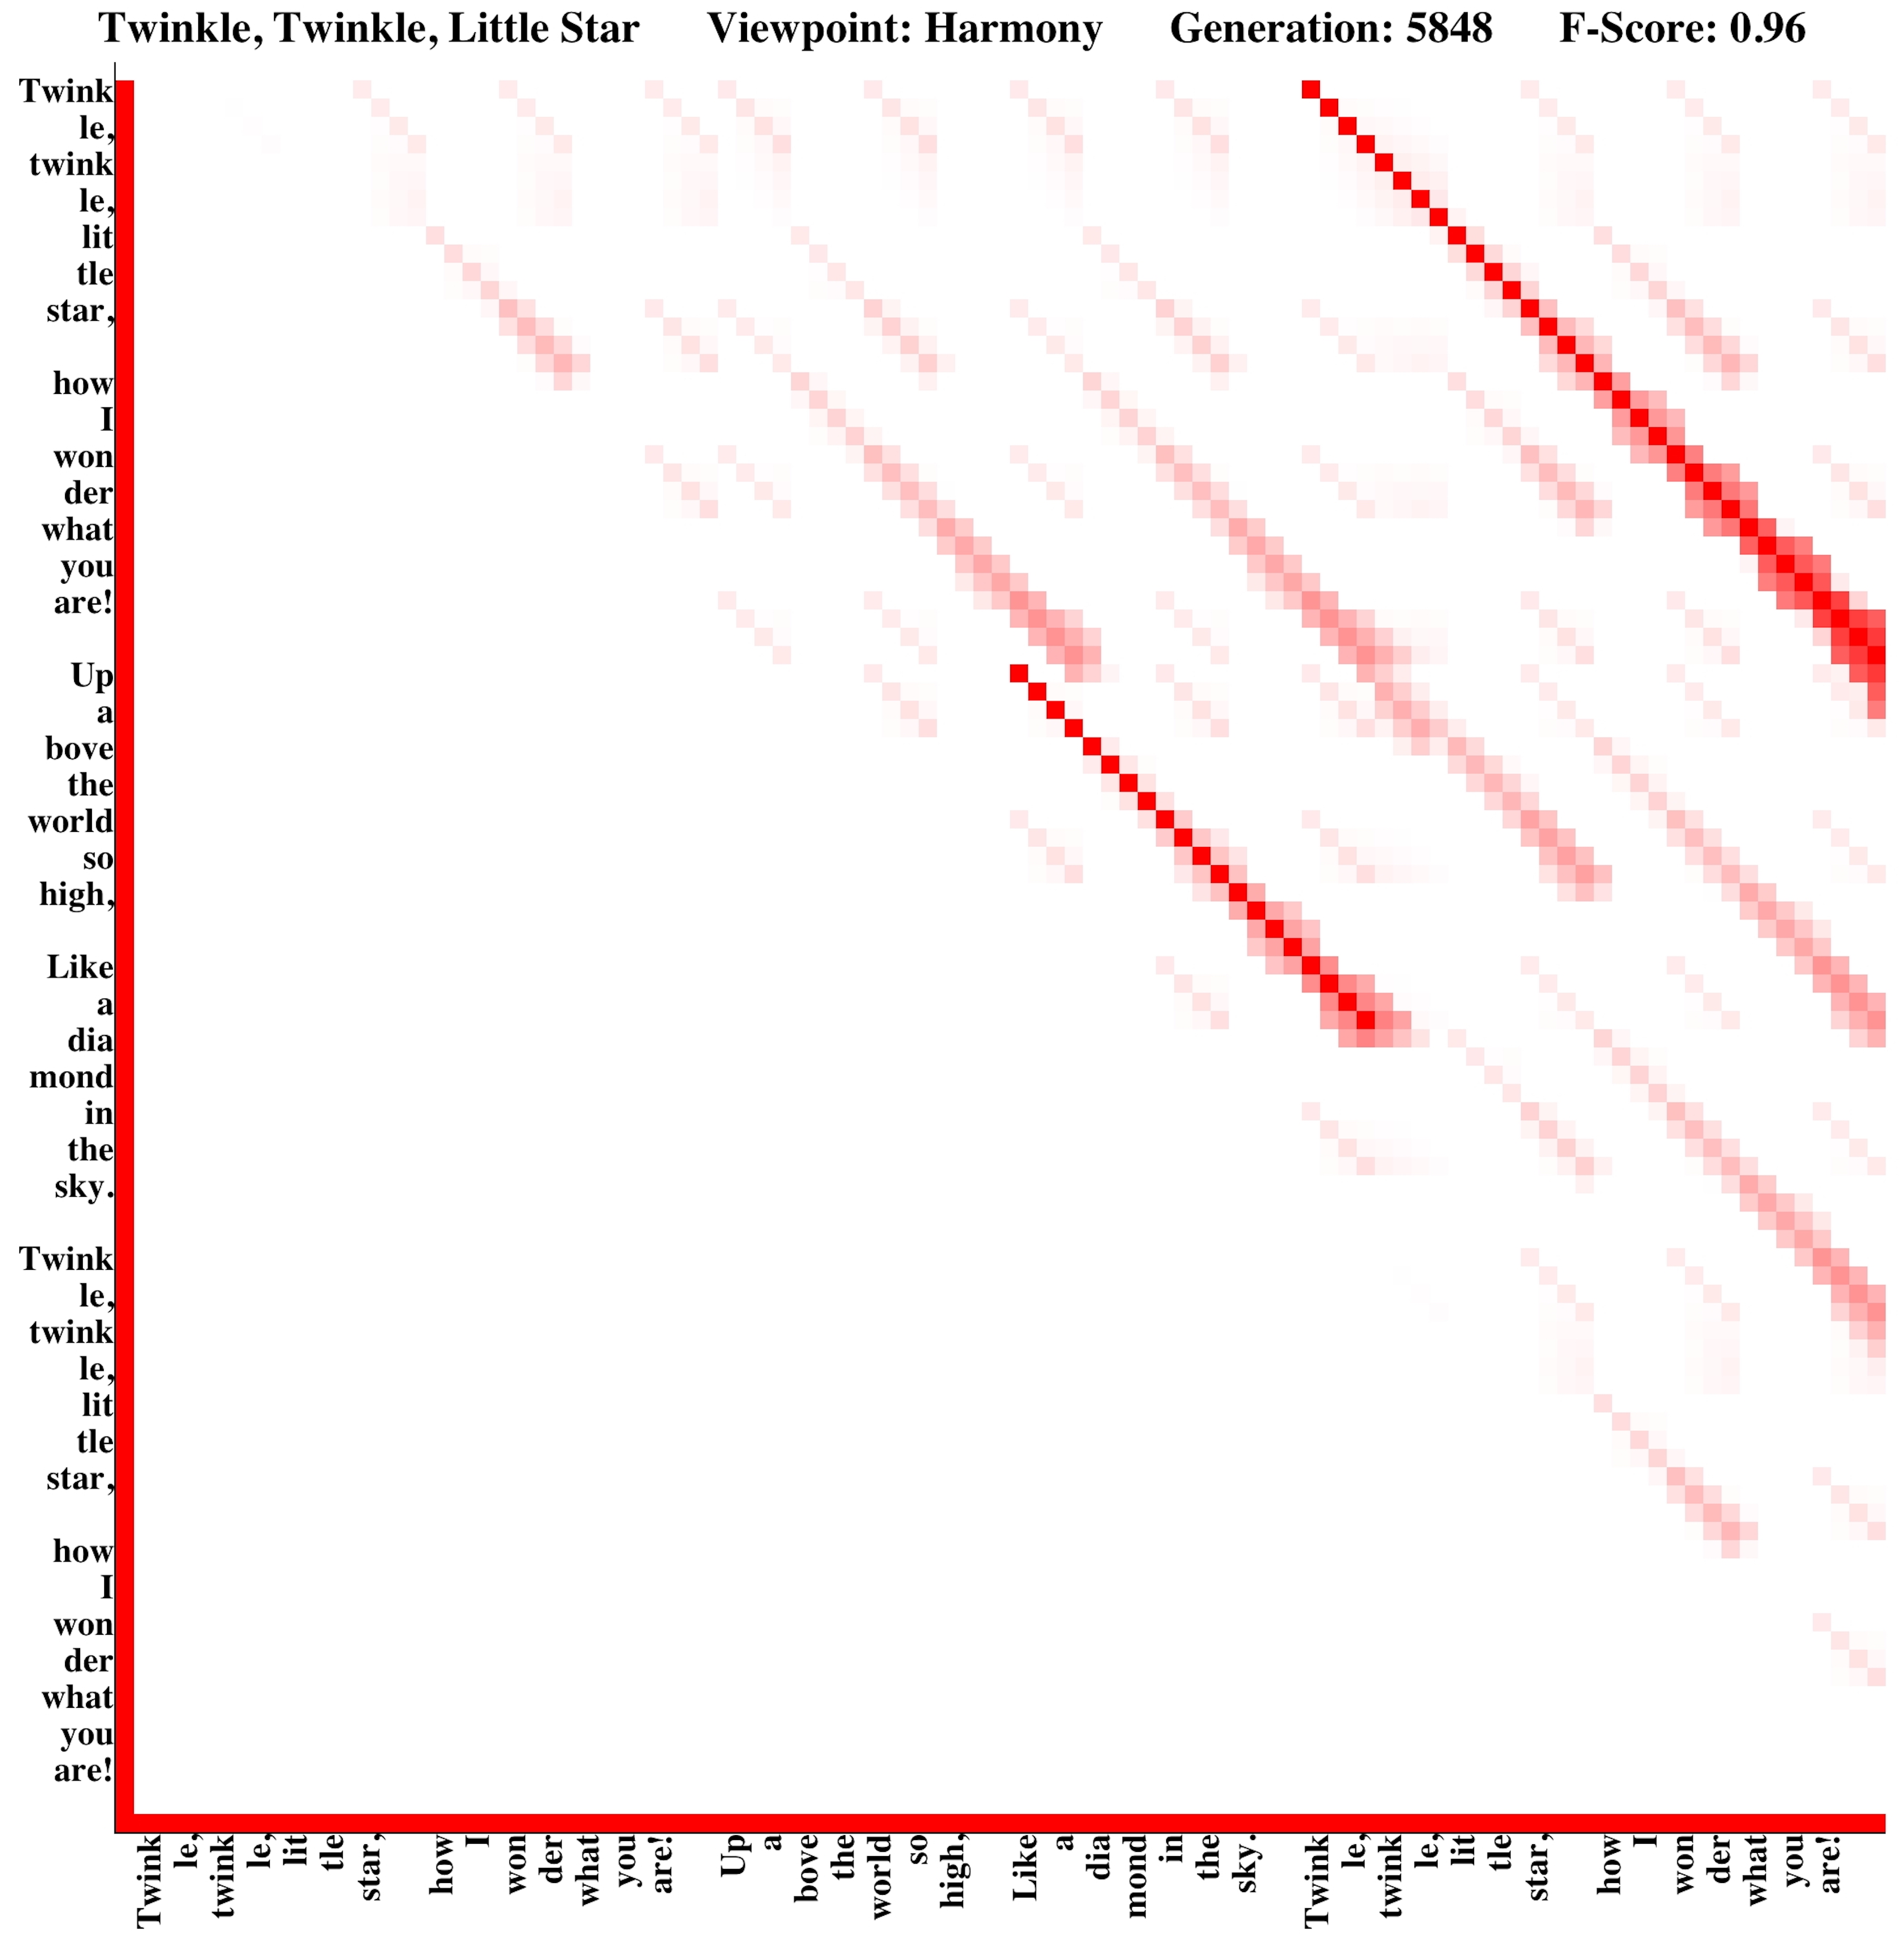
\includegraphics[width=\colwidth]{Twinkle__Twinkle__Little_Star_gen5848_id631_harmony} & 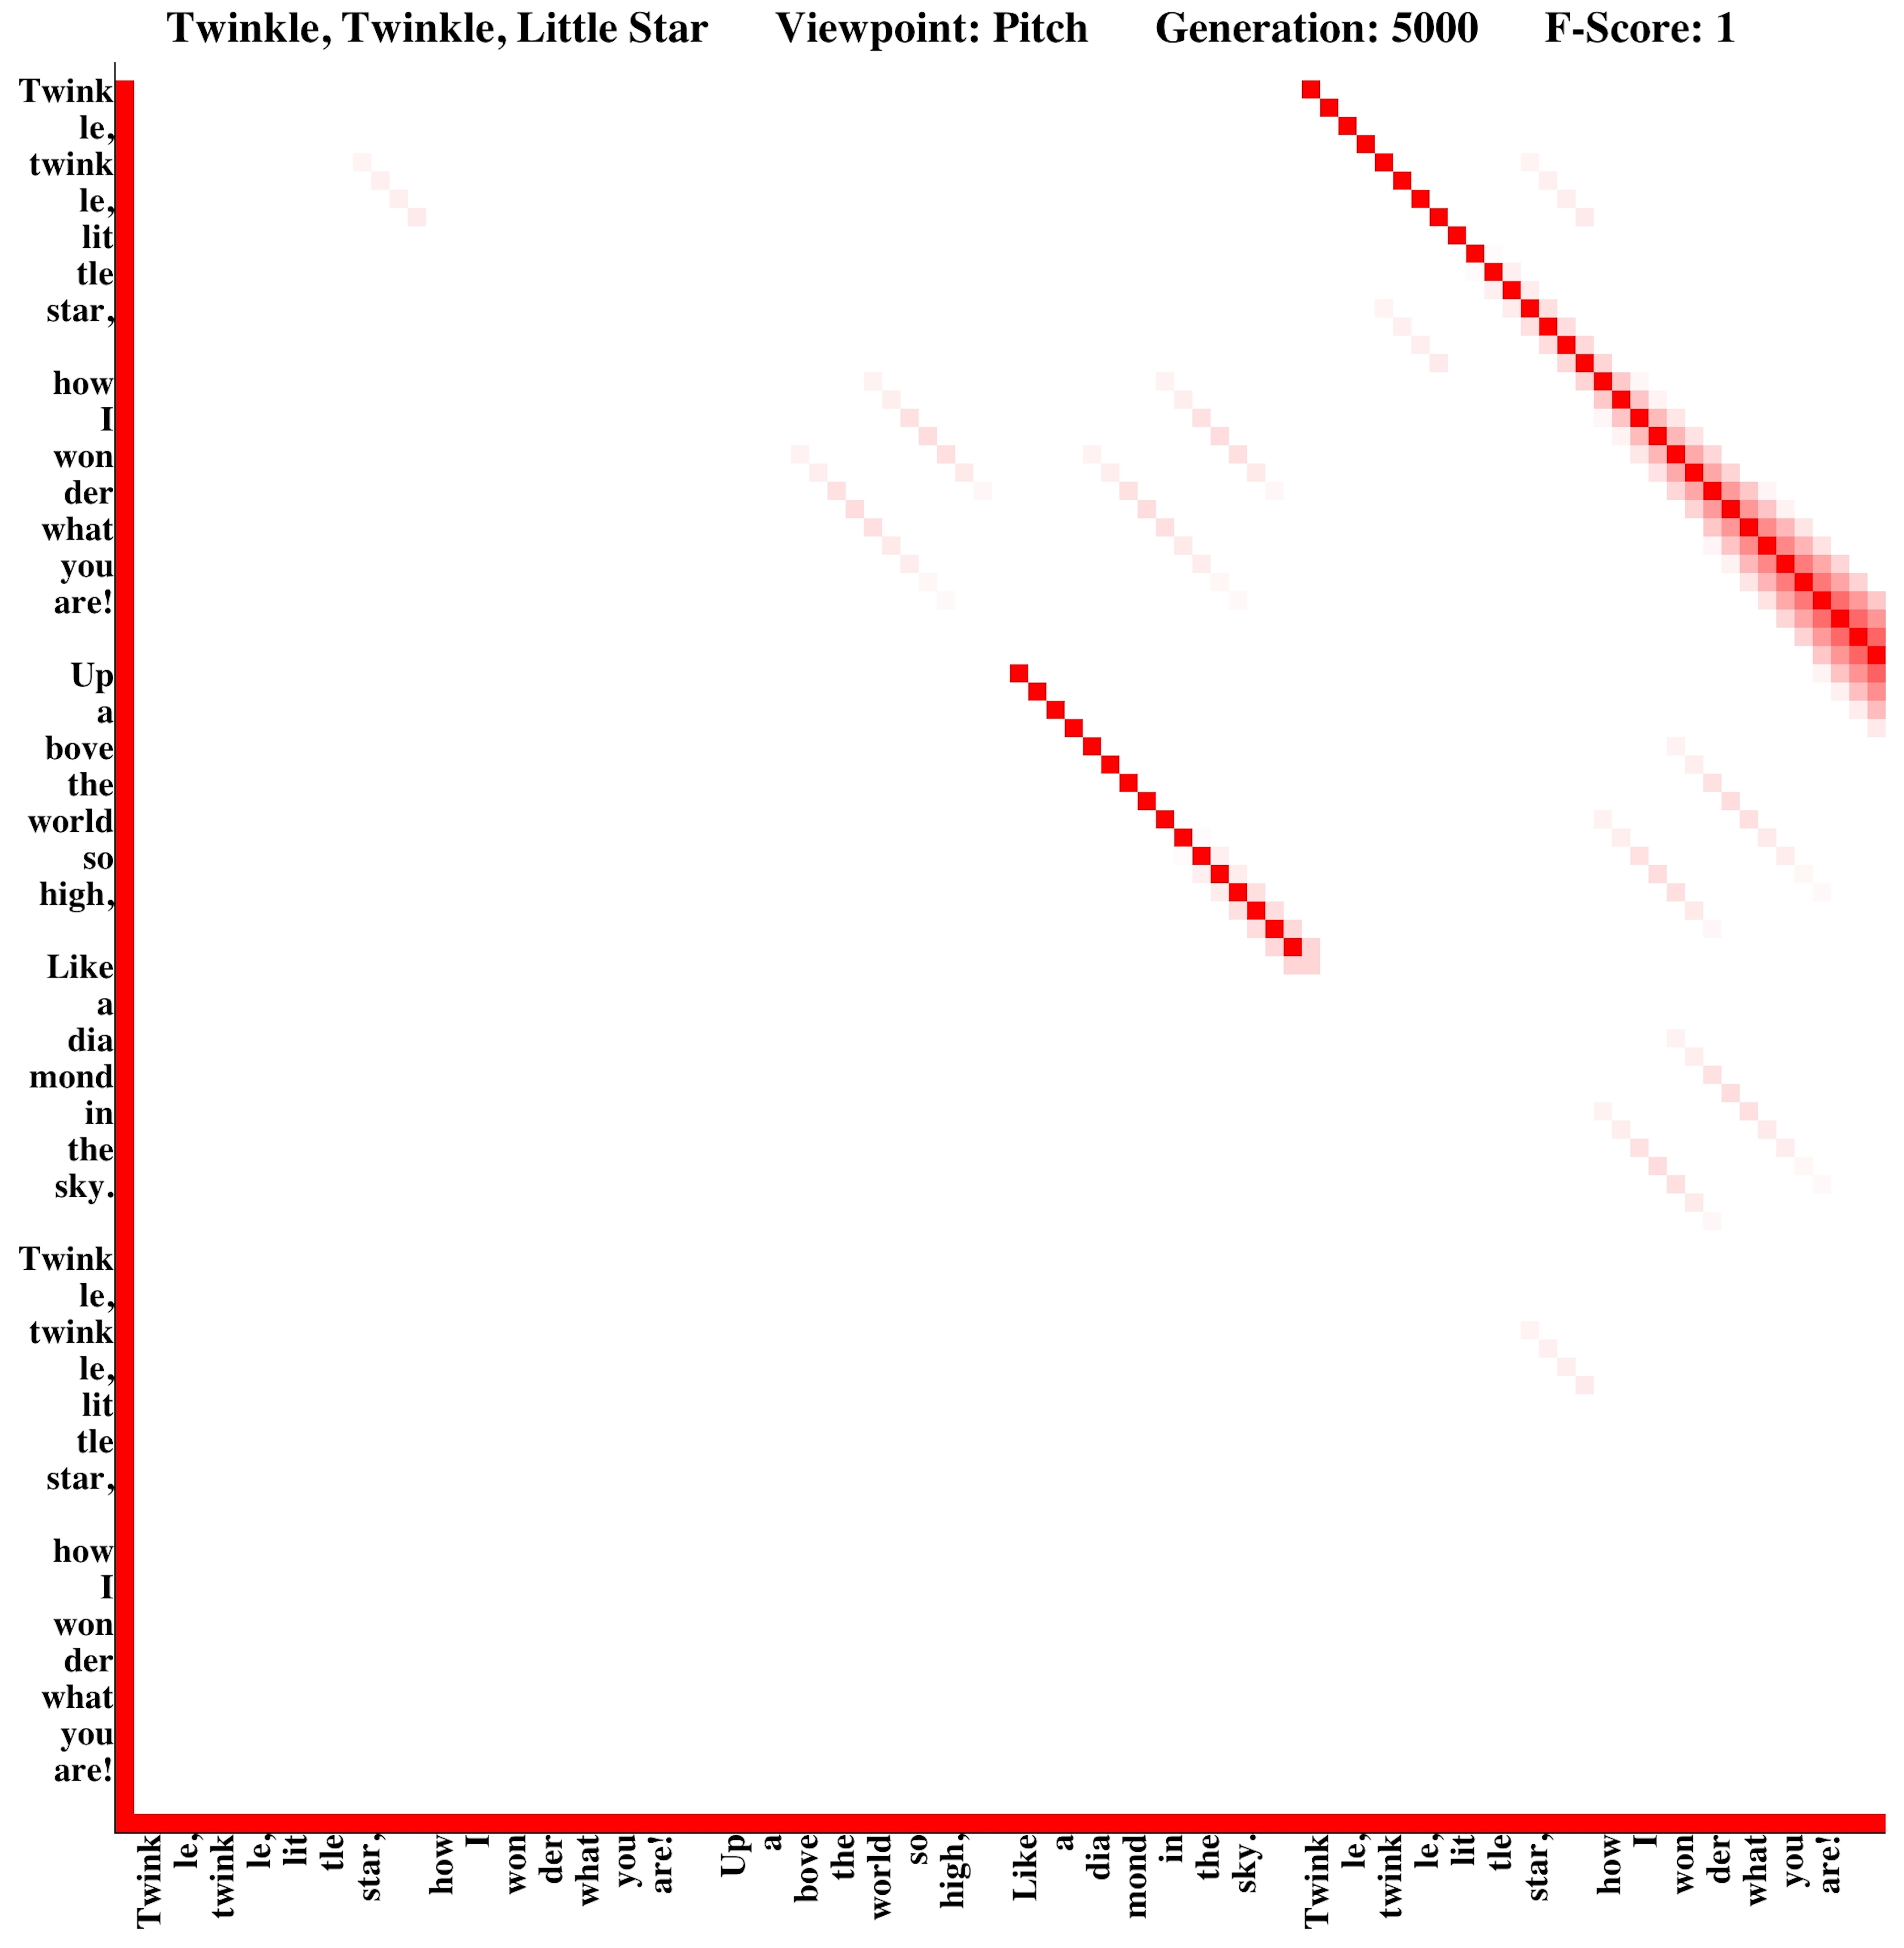
\includegraphics[width=\colwidth]{Twinkle__Twinkle__Little_Star_gen5000_id544_pitch} & 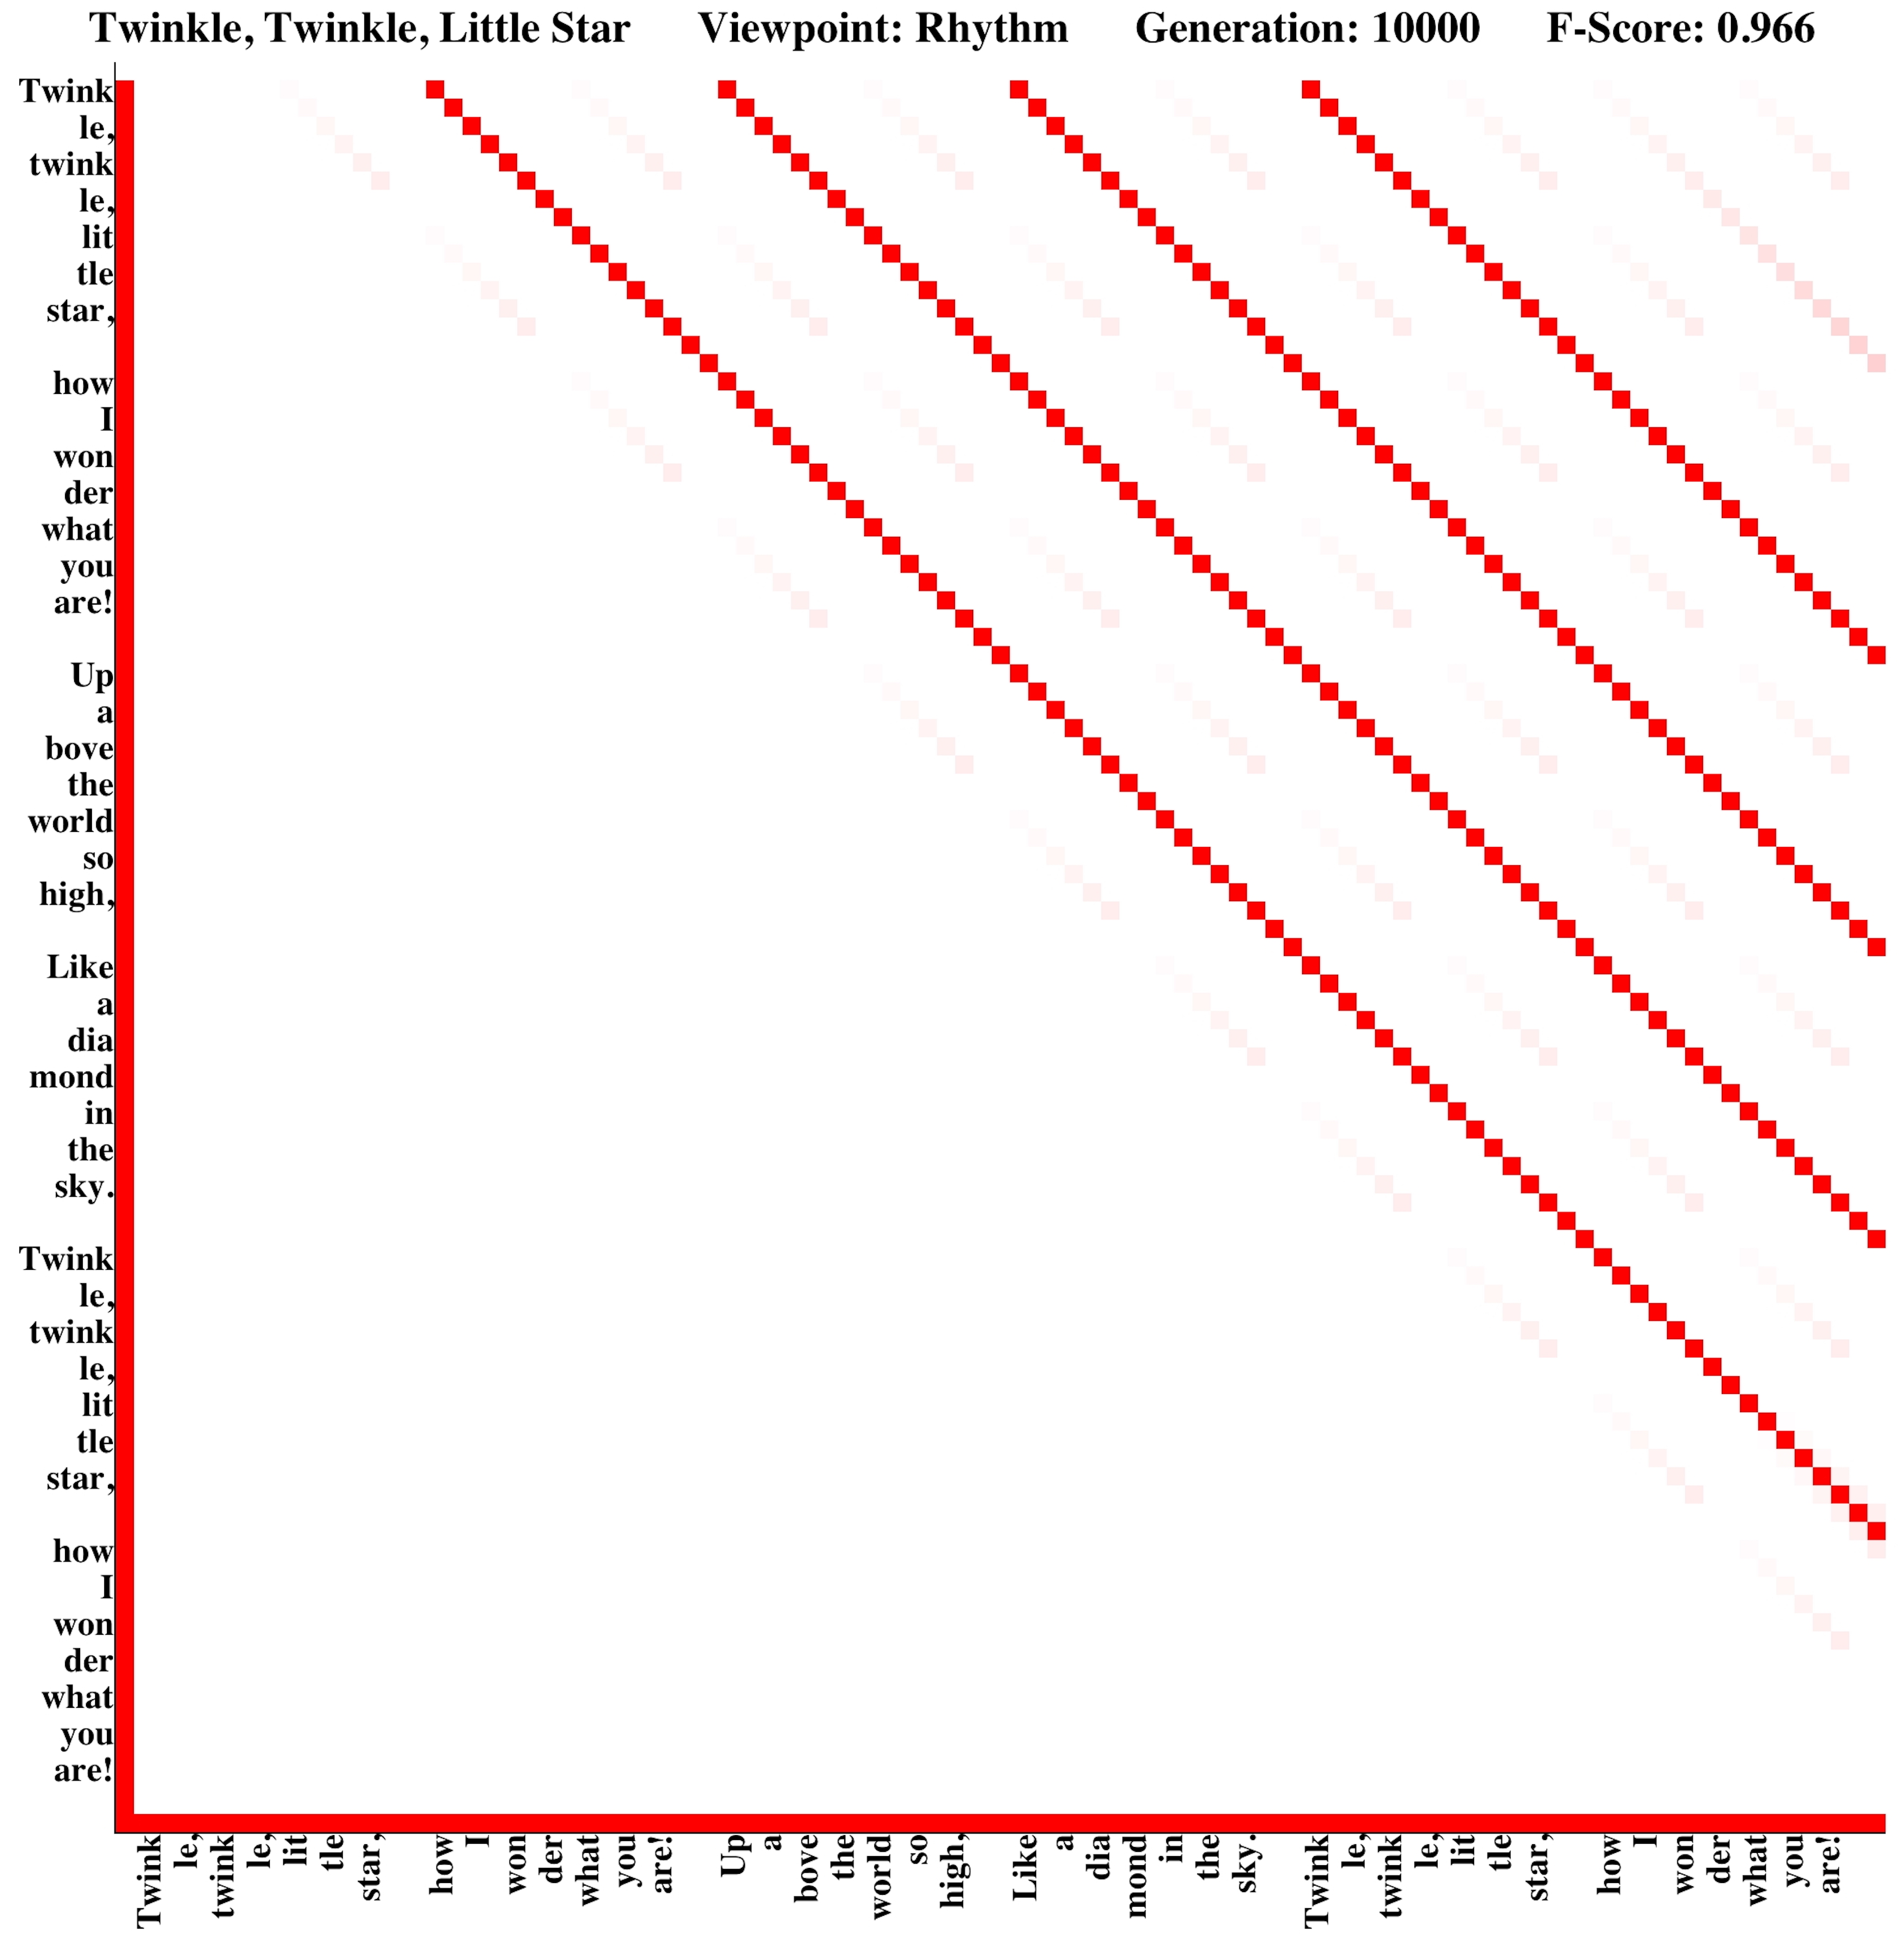
\includegraphics[width=\colwidth]{Twinkle__Twinkle__Little_Star_gen10000_id784_rhythm} & 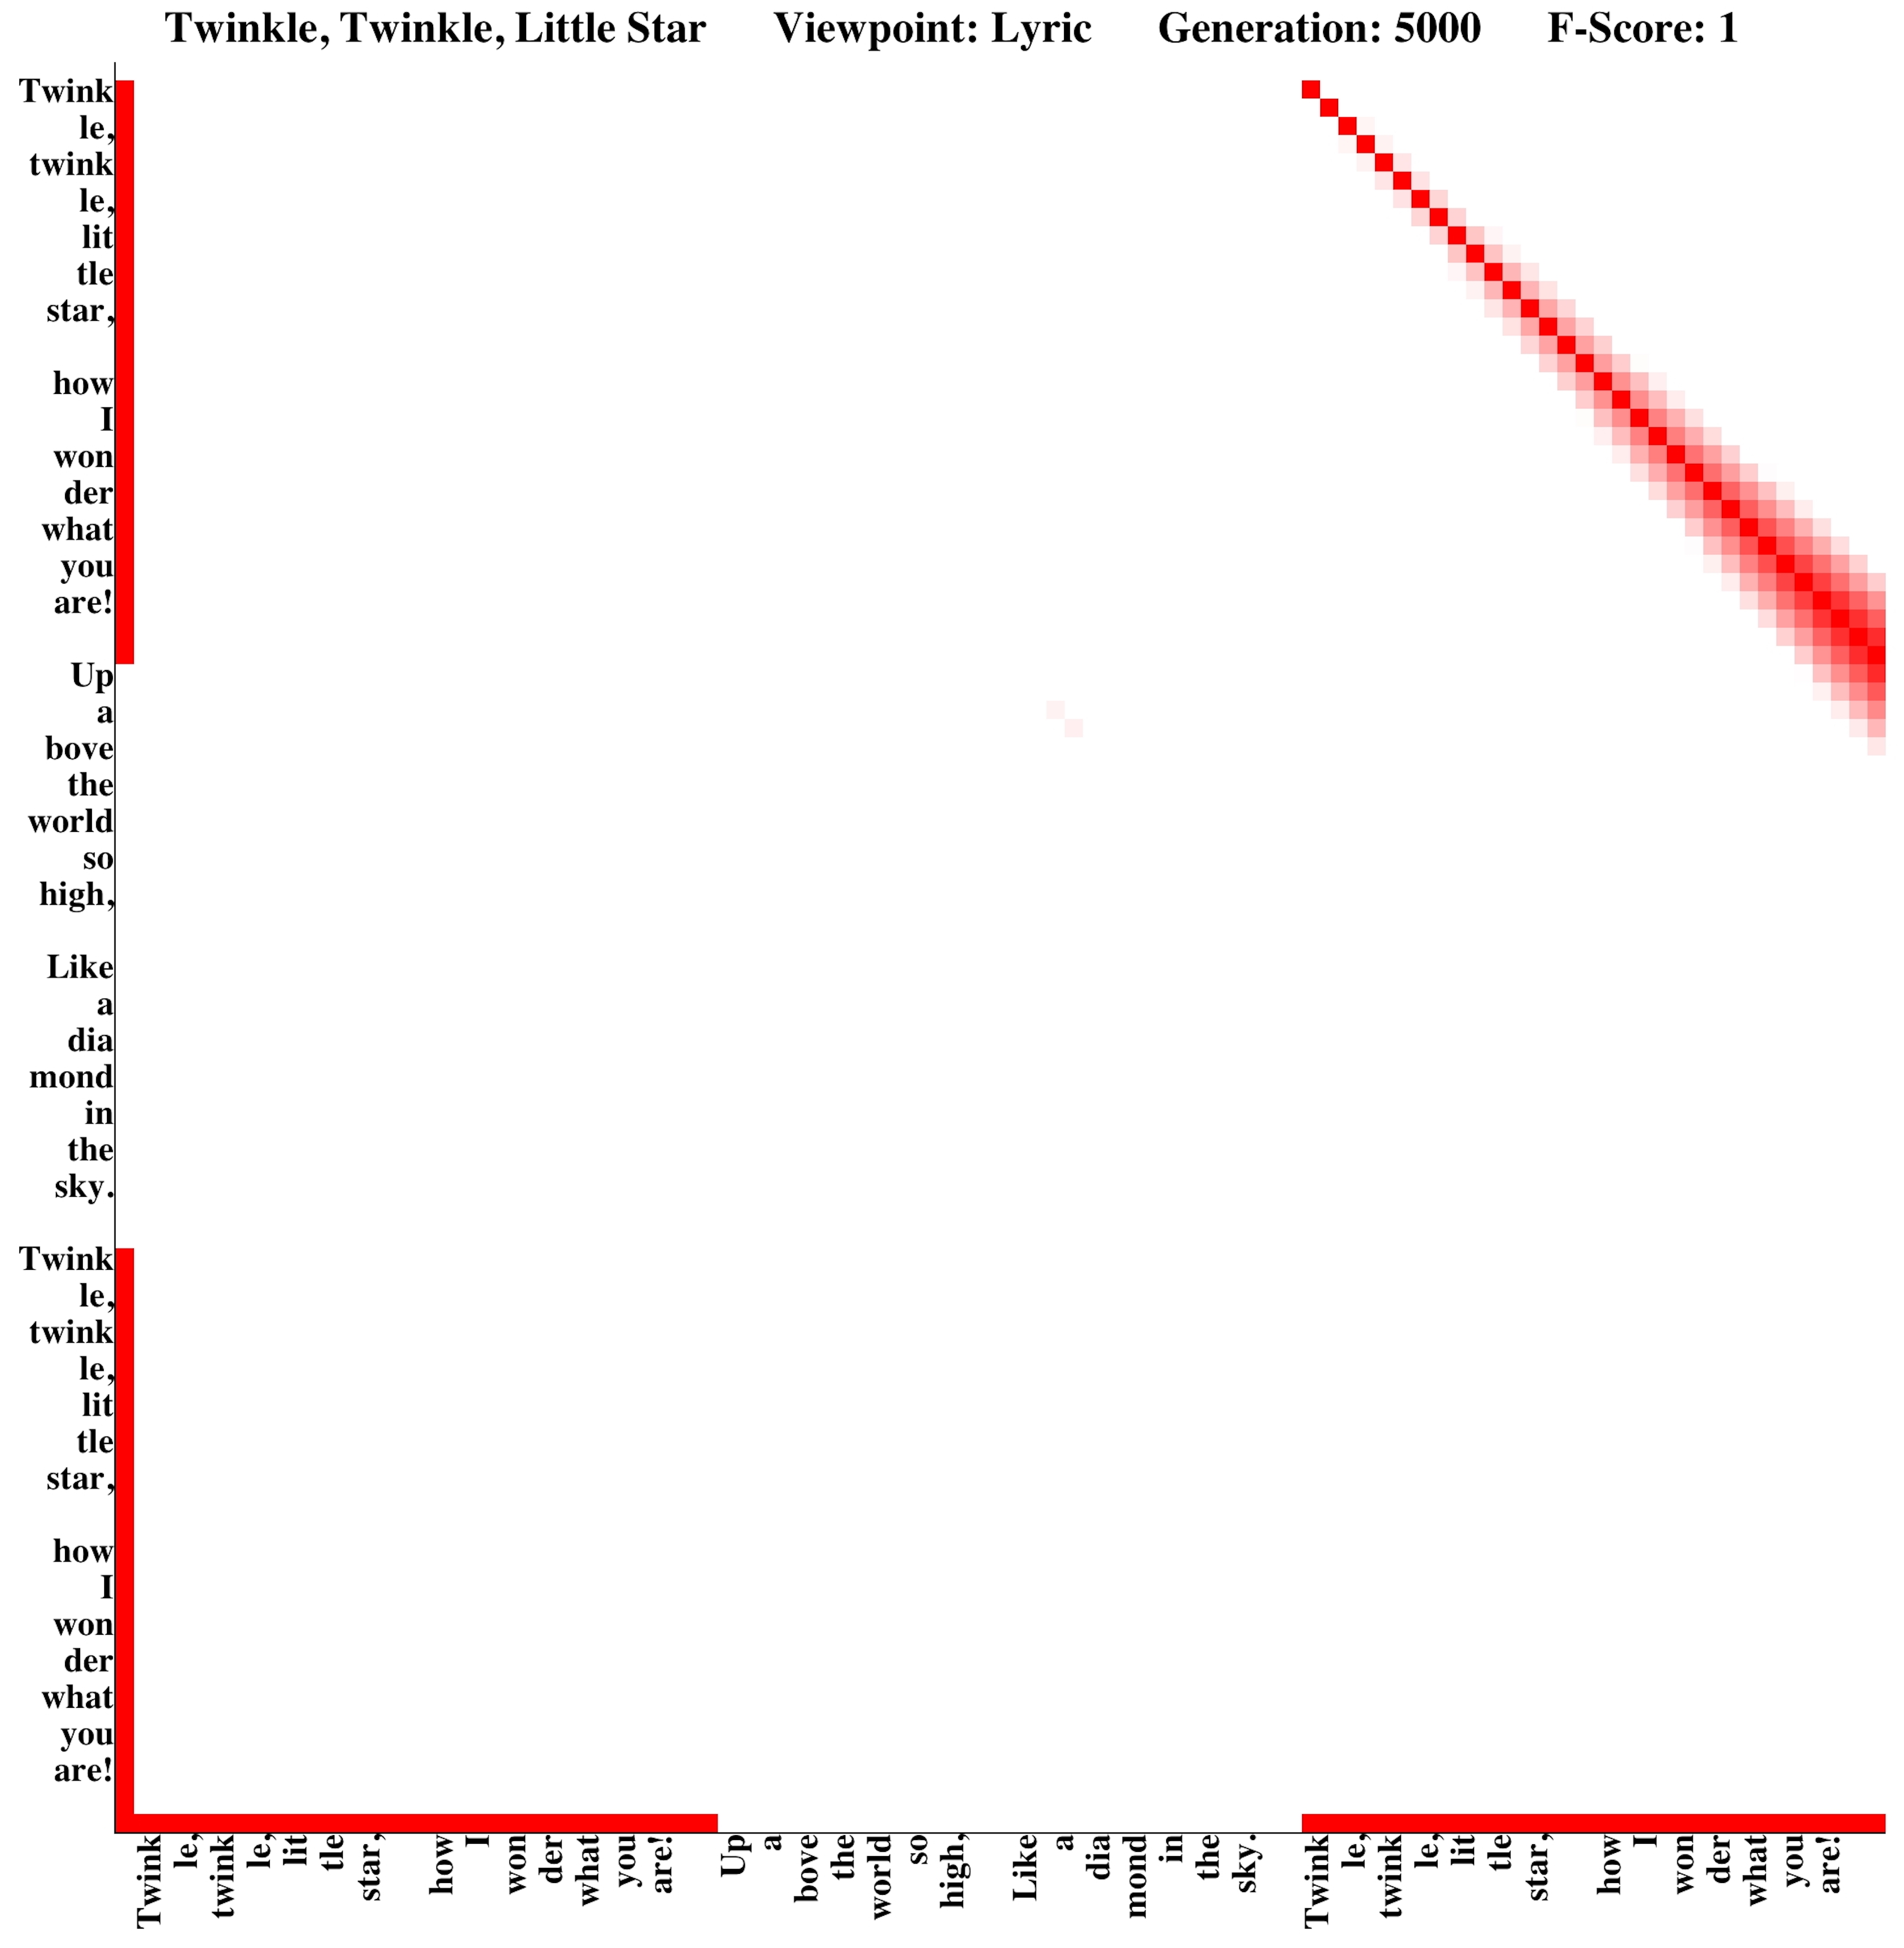
\includegraphics[width=\colwidth]{Twinkle__Twinkle__Little_Star_gen5000_id435_lyric} & 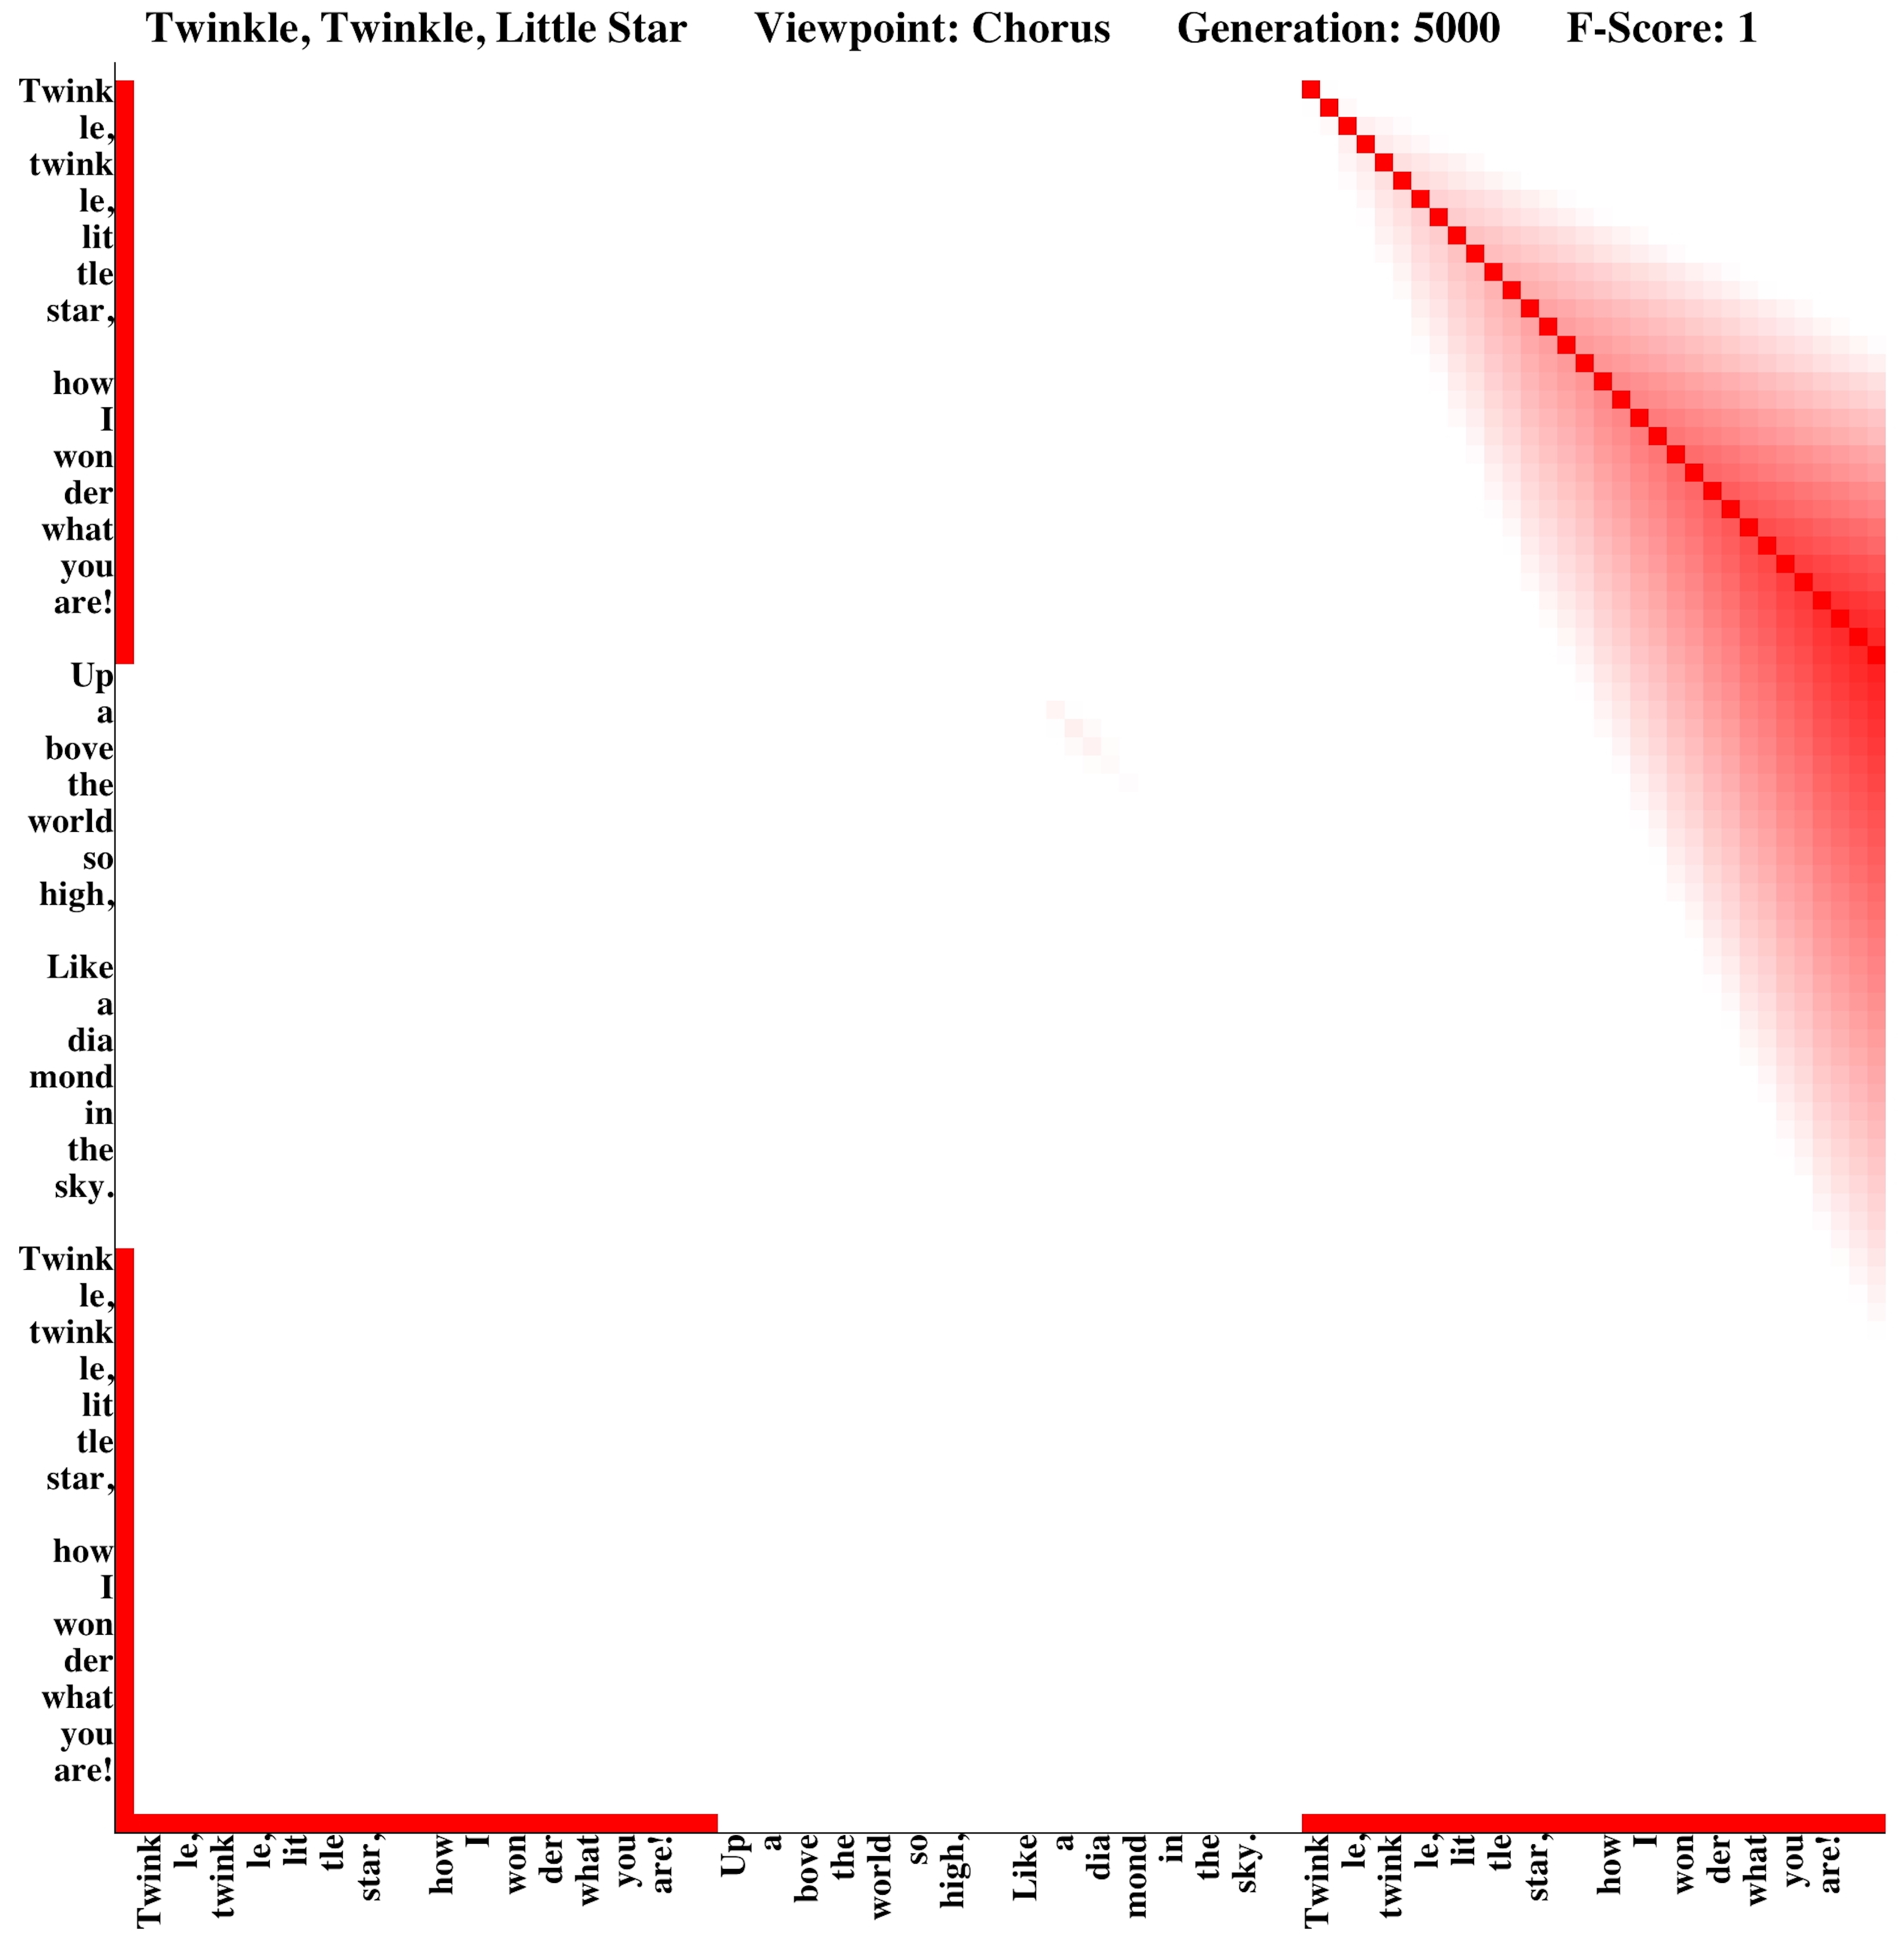
\includegraphics[width=\colwidth]{Twinkle__Twinkle__Little_Star_gen5000_id399_chorus} & 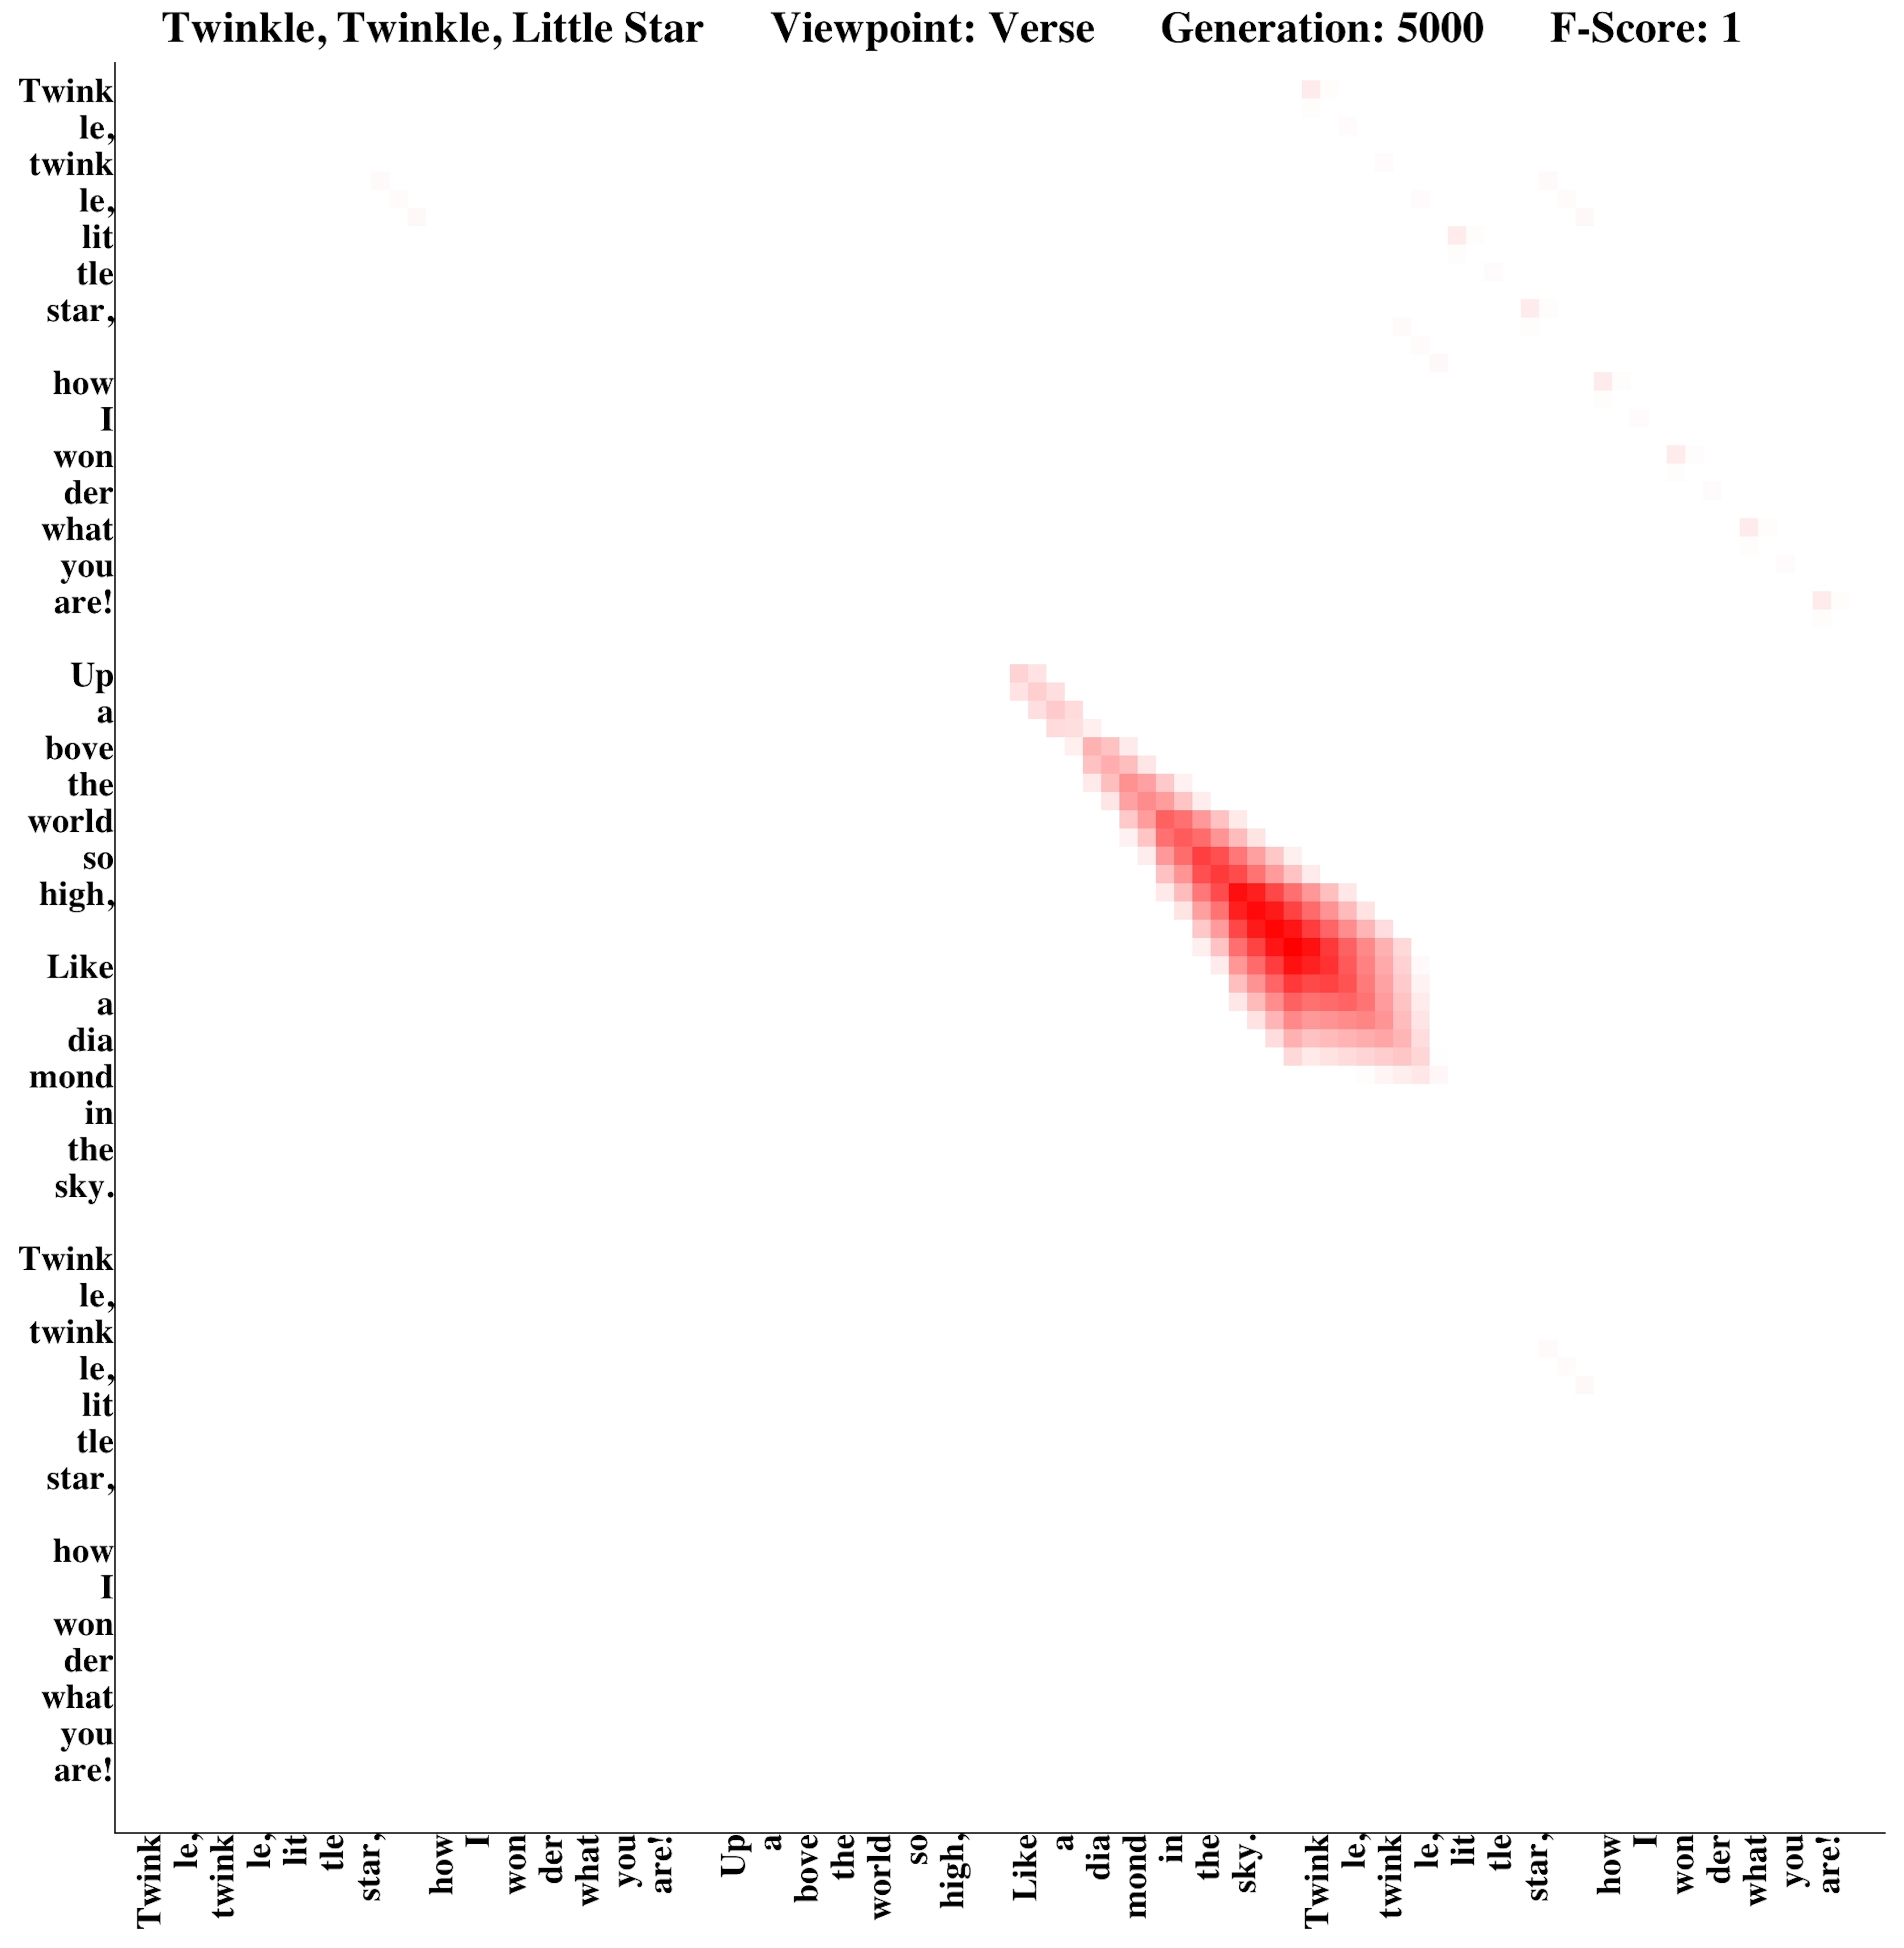
\includegraphics[width=\colwidth]{Twinkle__Twinkle__Little_Star_gen5000_id467_verse} \\
% & F-Score:0.96 & F-Score:1.00 & F-Score:1.00 & F-Score:1.00 & F-Score:1.00 & F-Score:0.00 \\
\textbf{Over the Rainbow} $F_{1}=0.97$ & 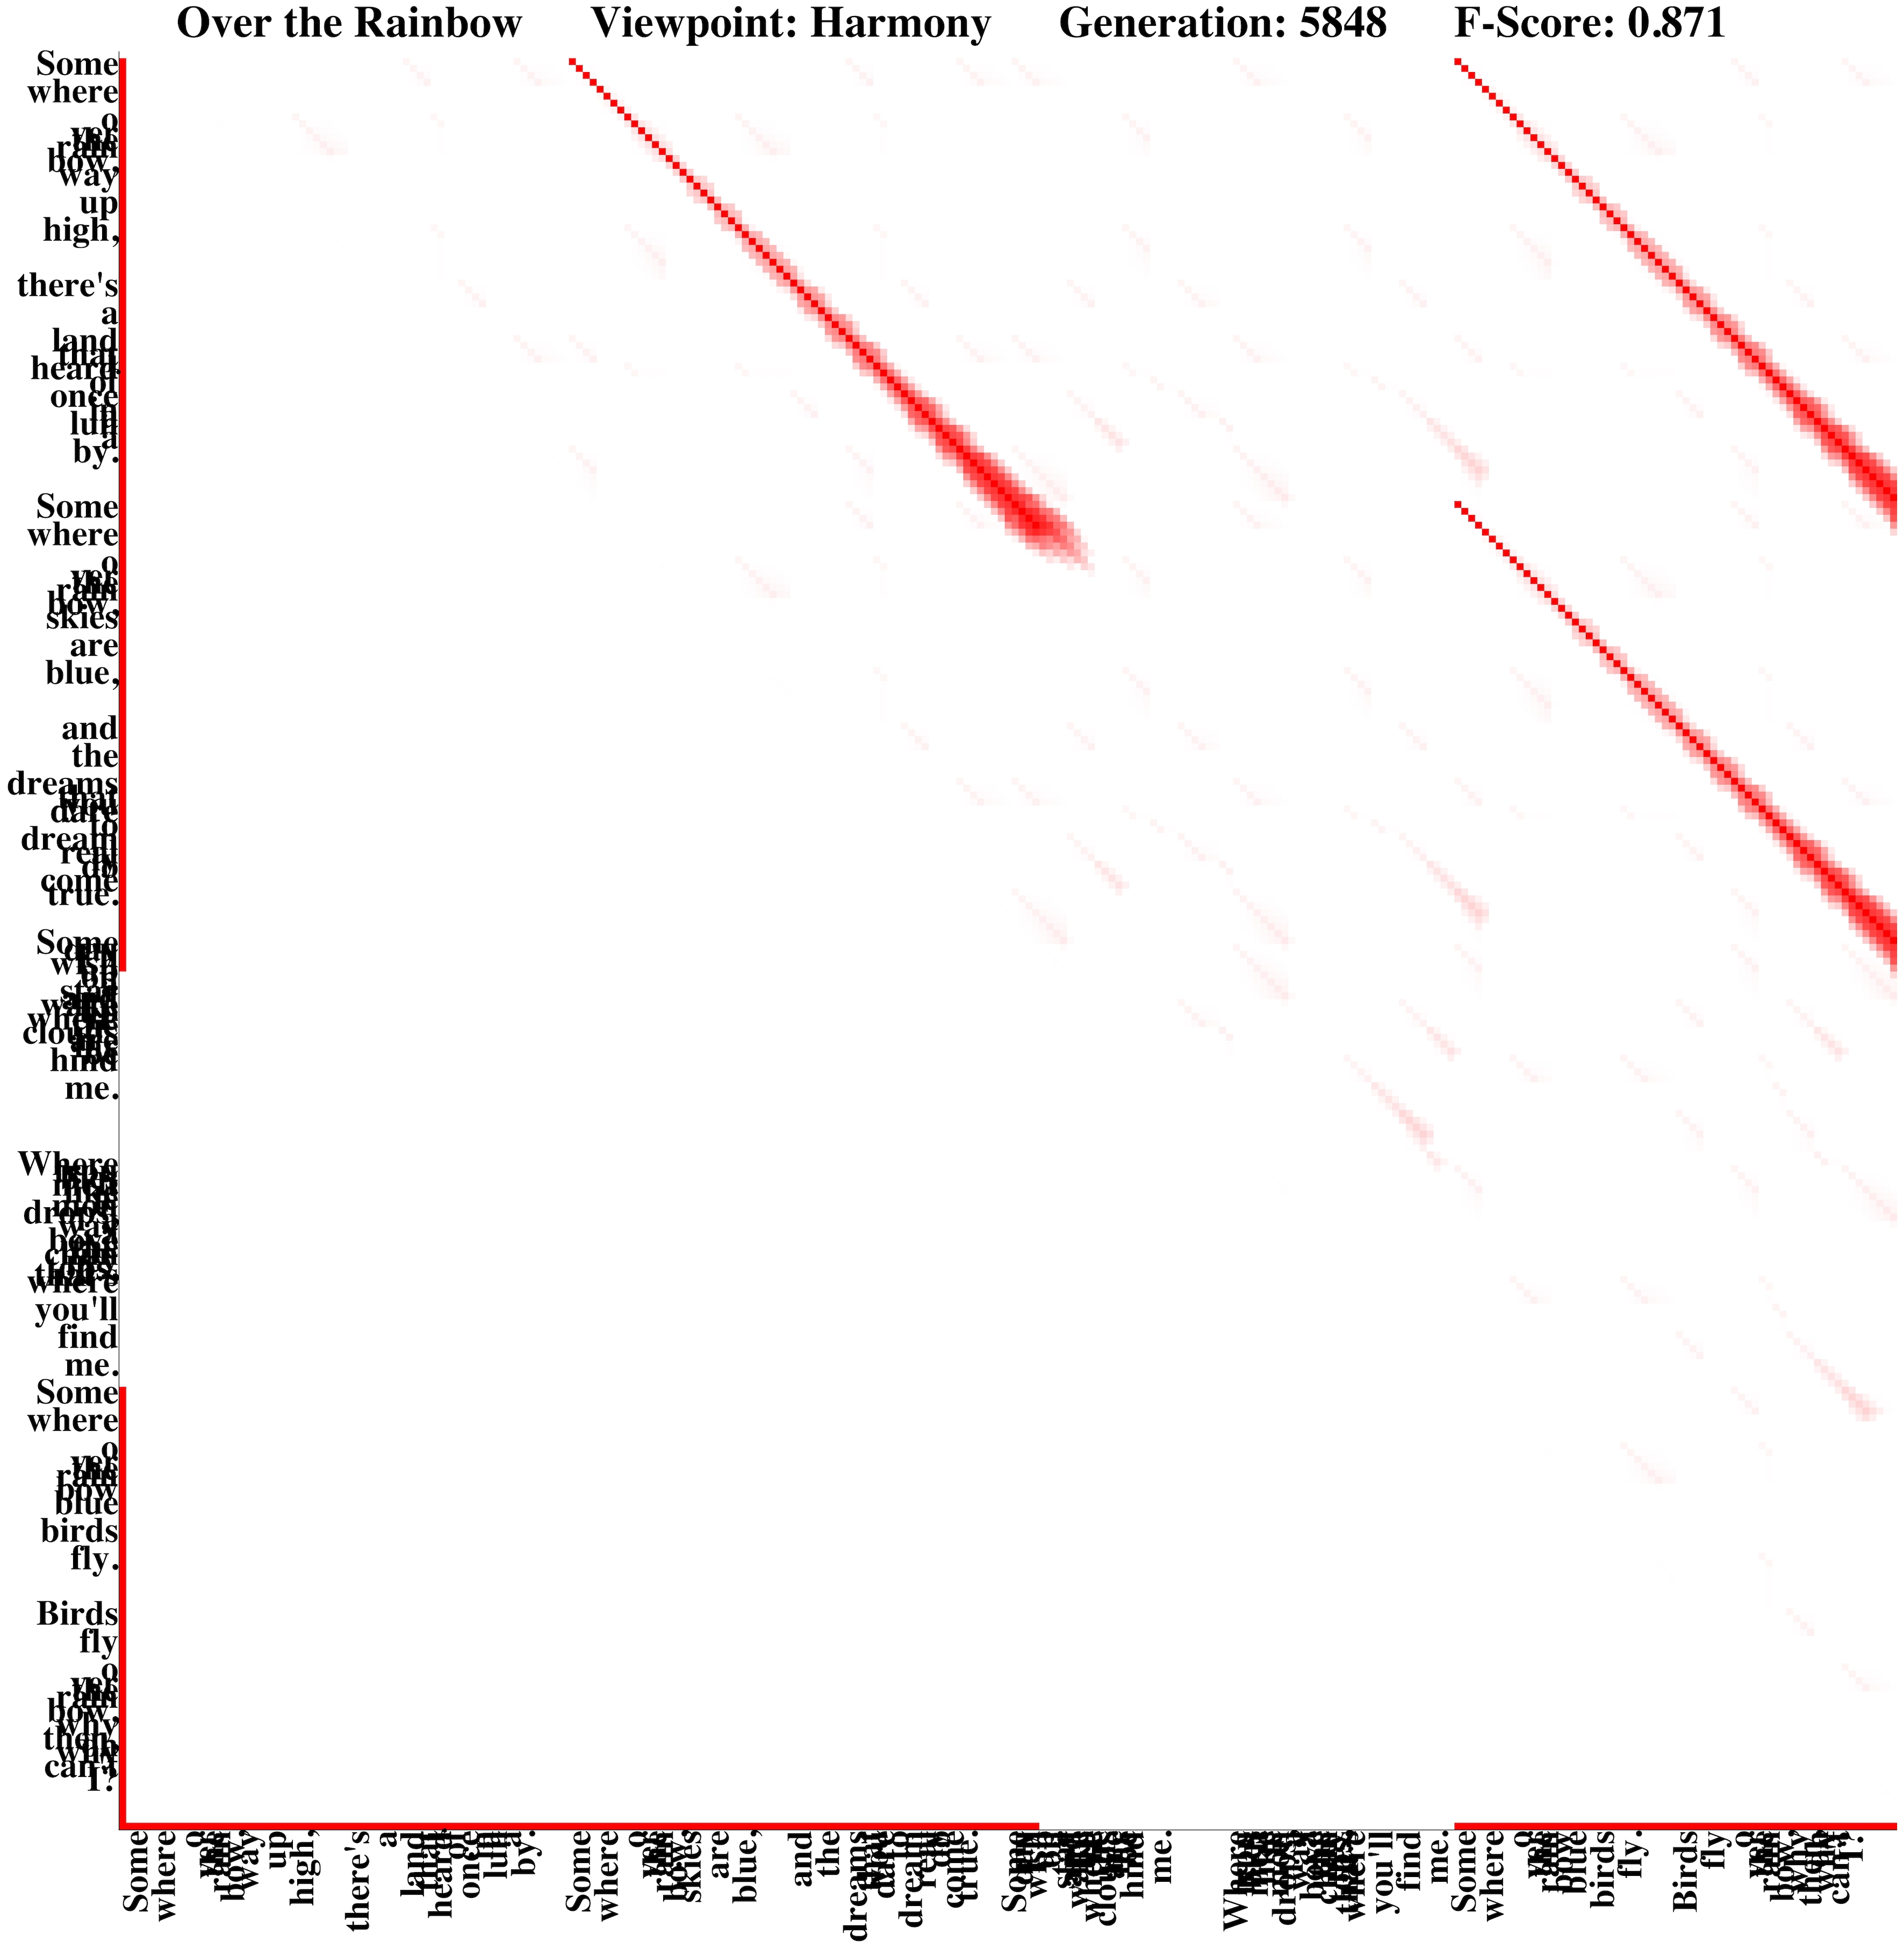
\includegraphics[width=\colwidth]{Over_the_Rainbow_gen5848_id631_harmony} & 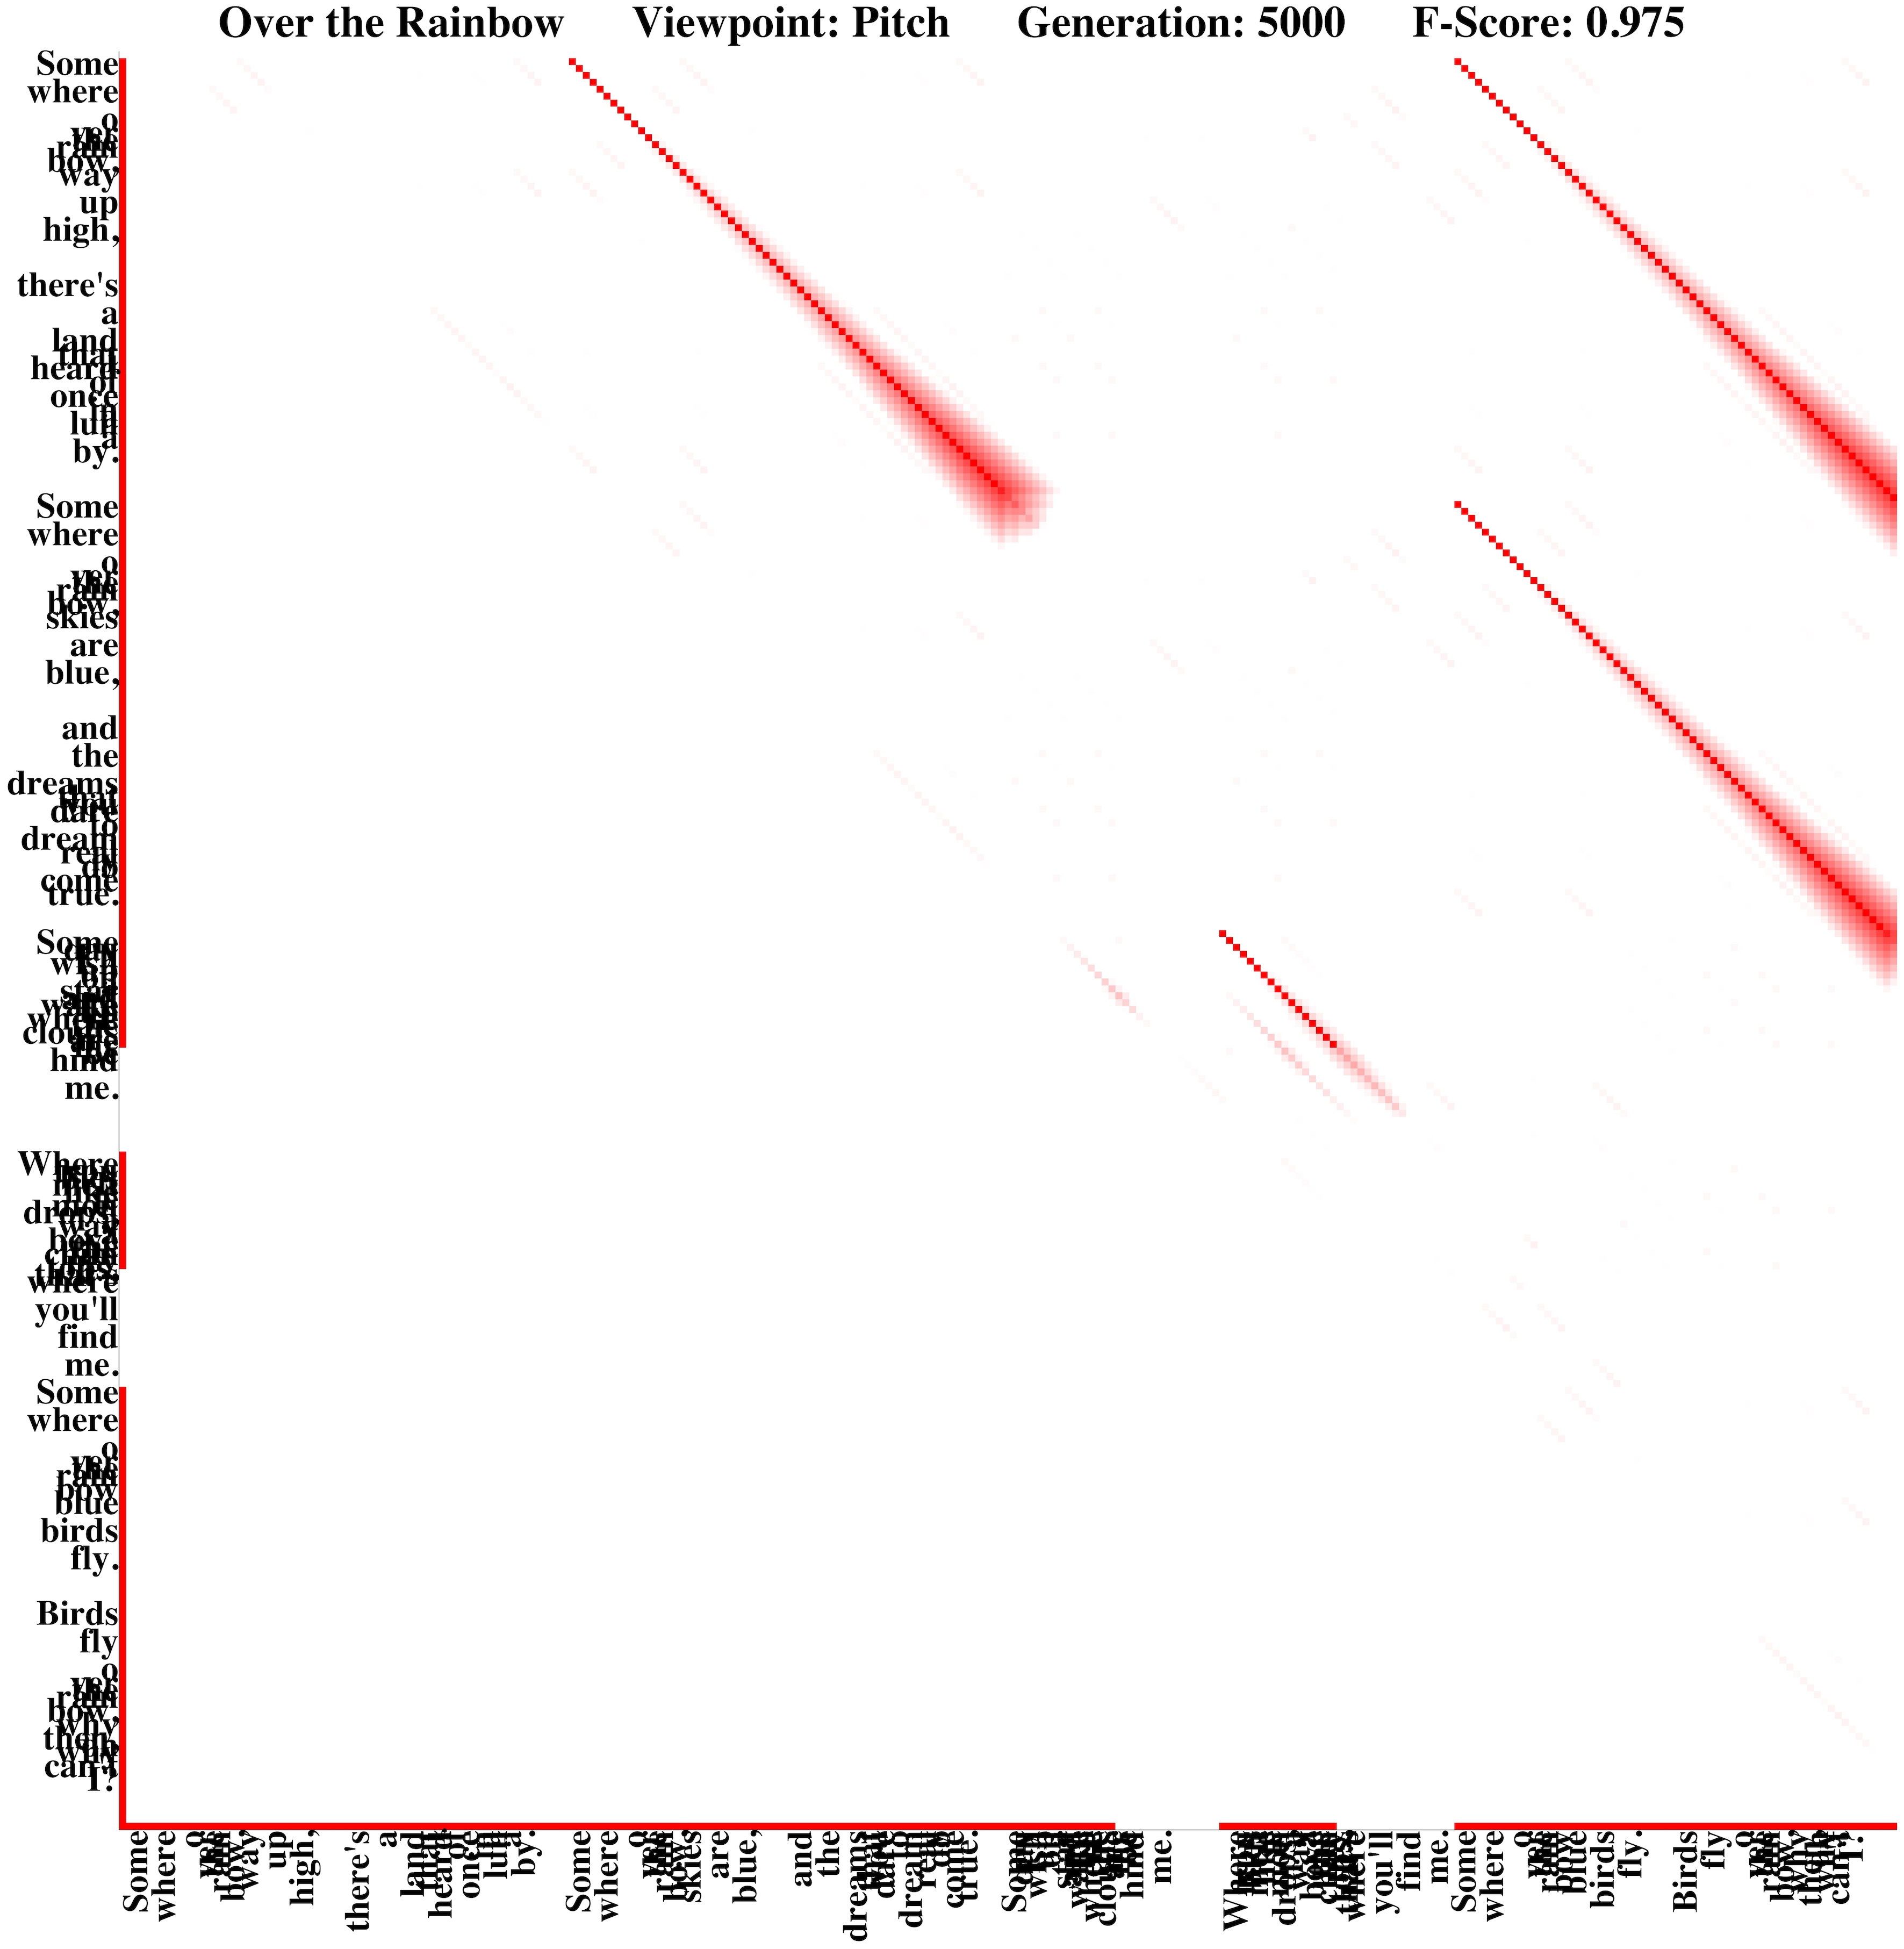
\includegraphics[width=\colwidth]{Over_the_Rainbow_gen5000_id544_pitch} & 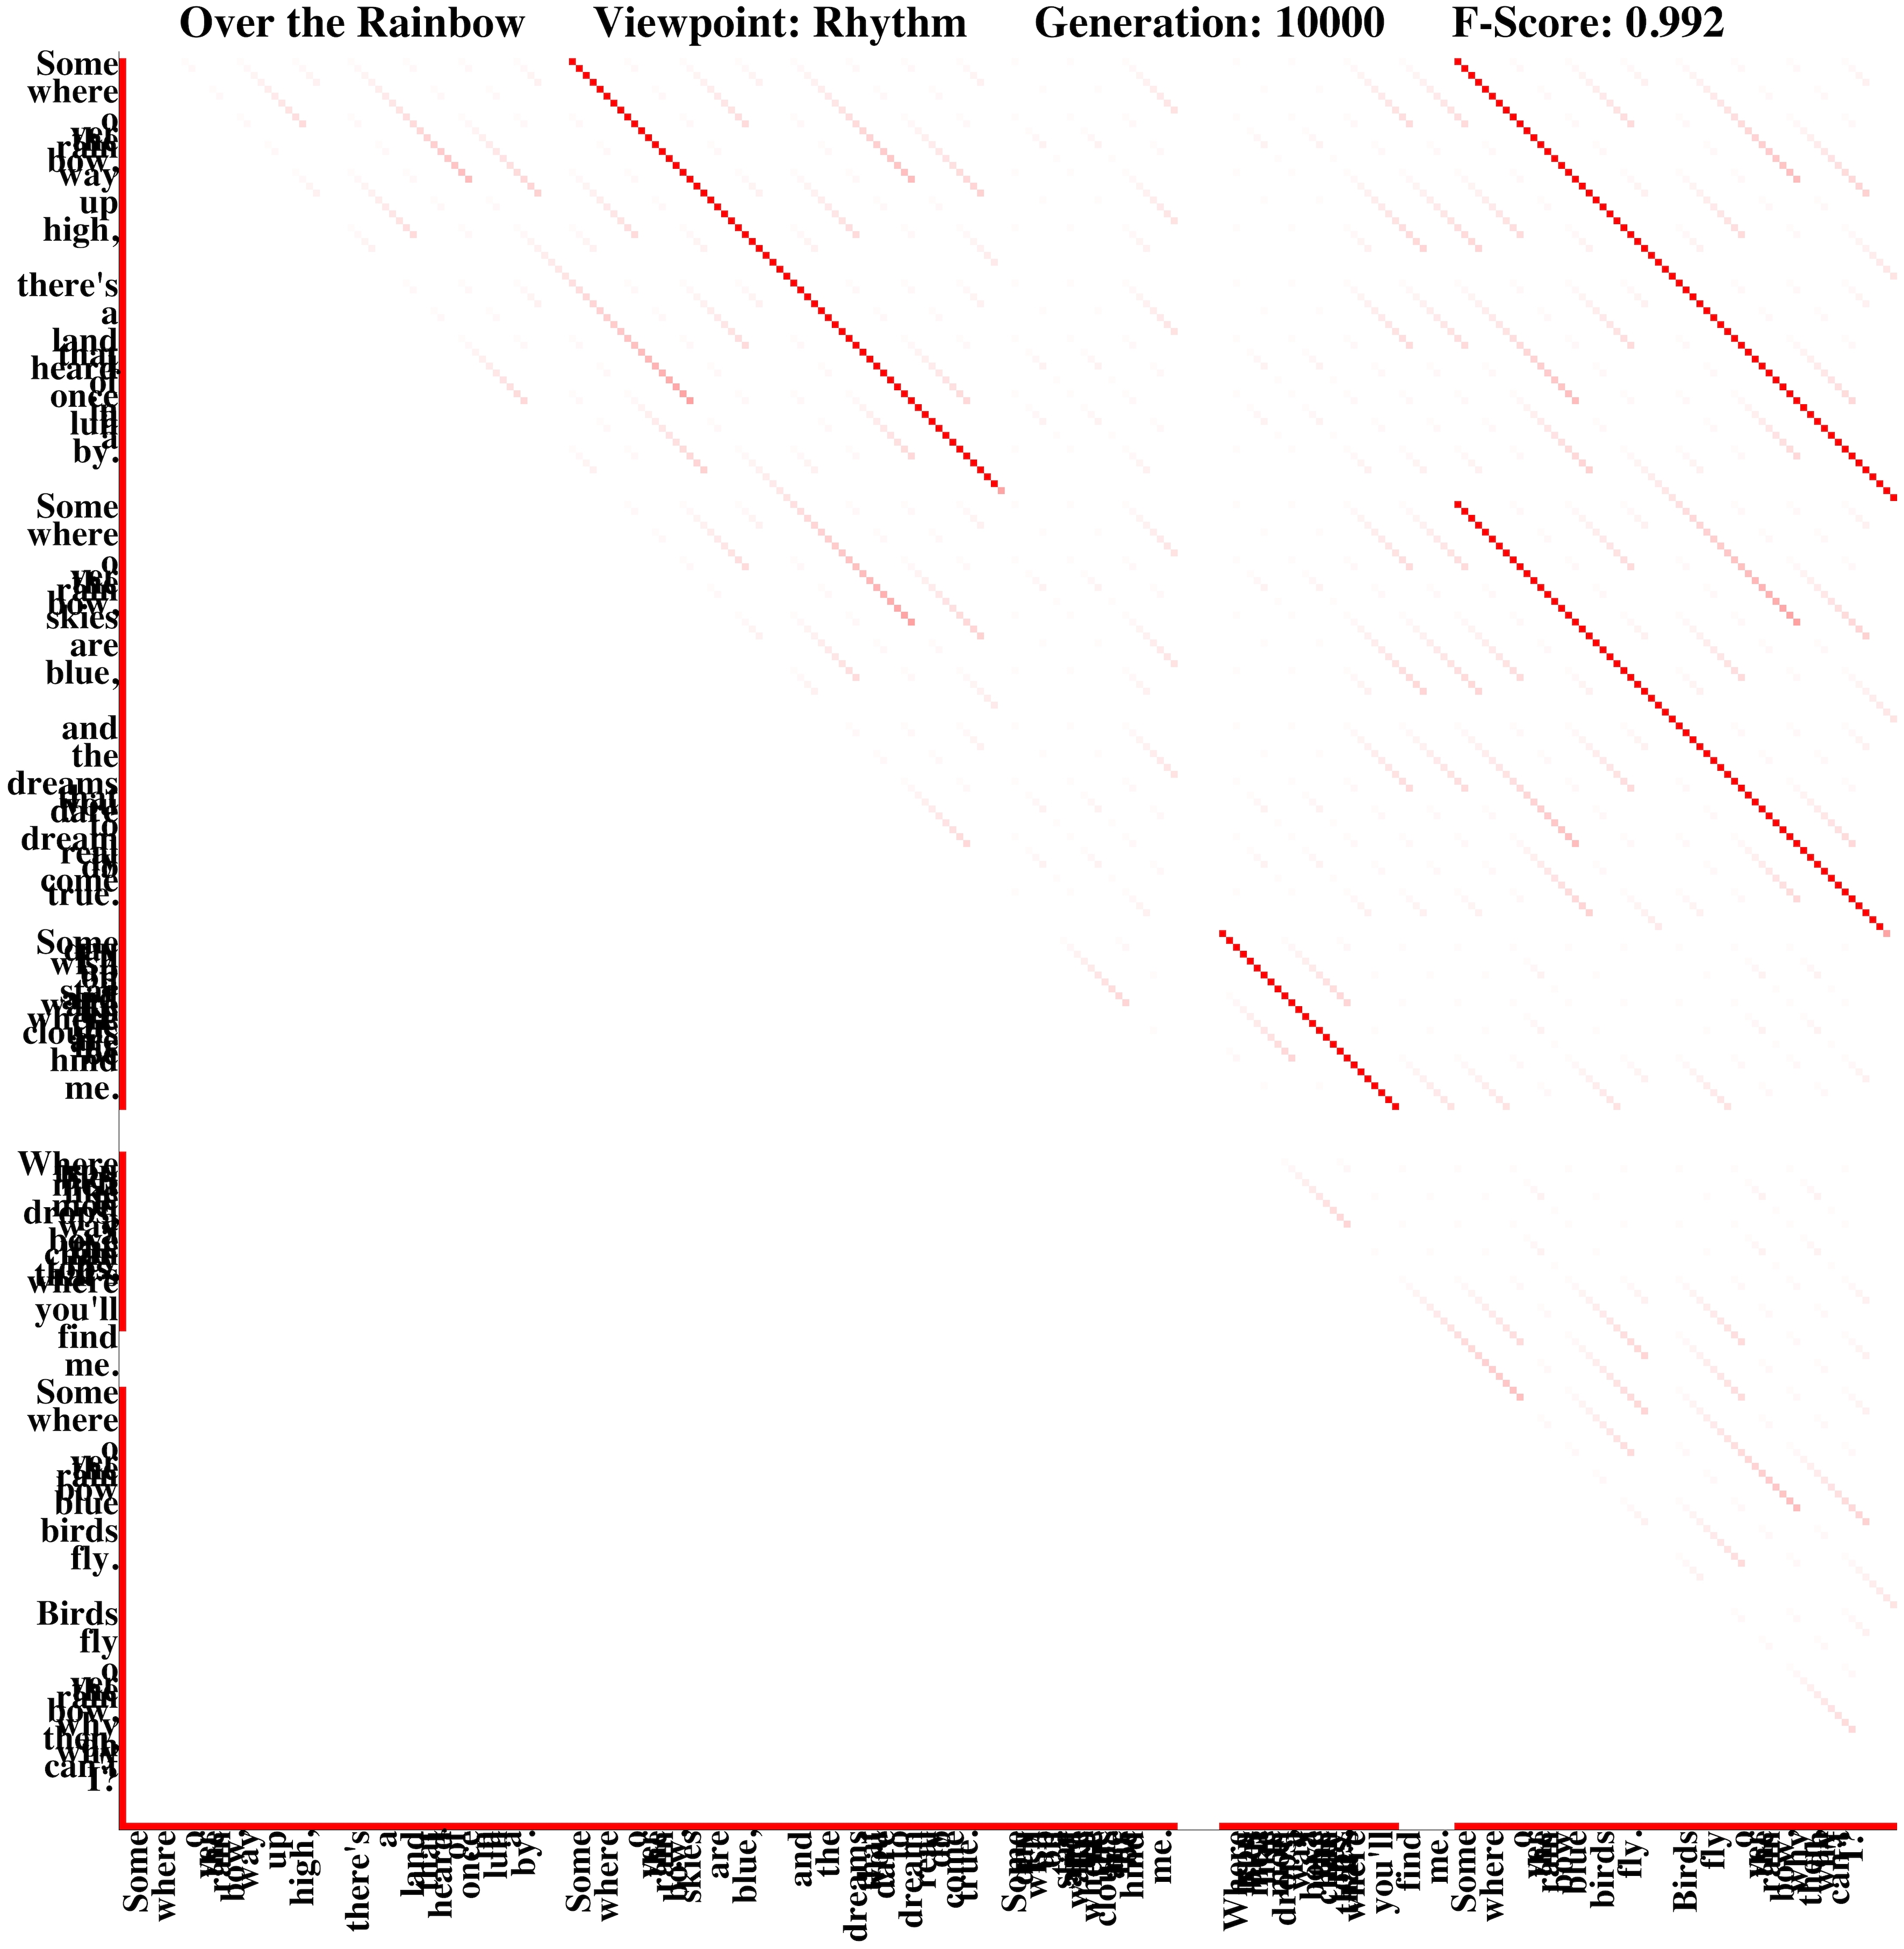
\includegraphics[width=\colwidth]{Over_the_Rainbow_gen10000_id784_rhythm} & 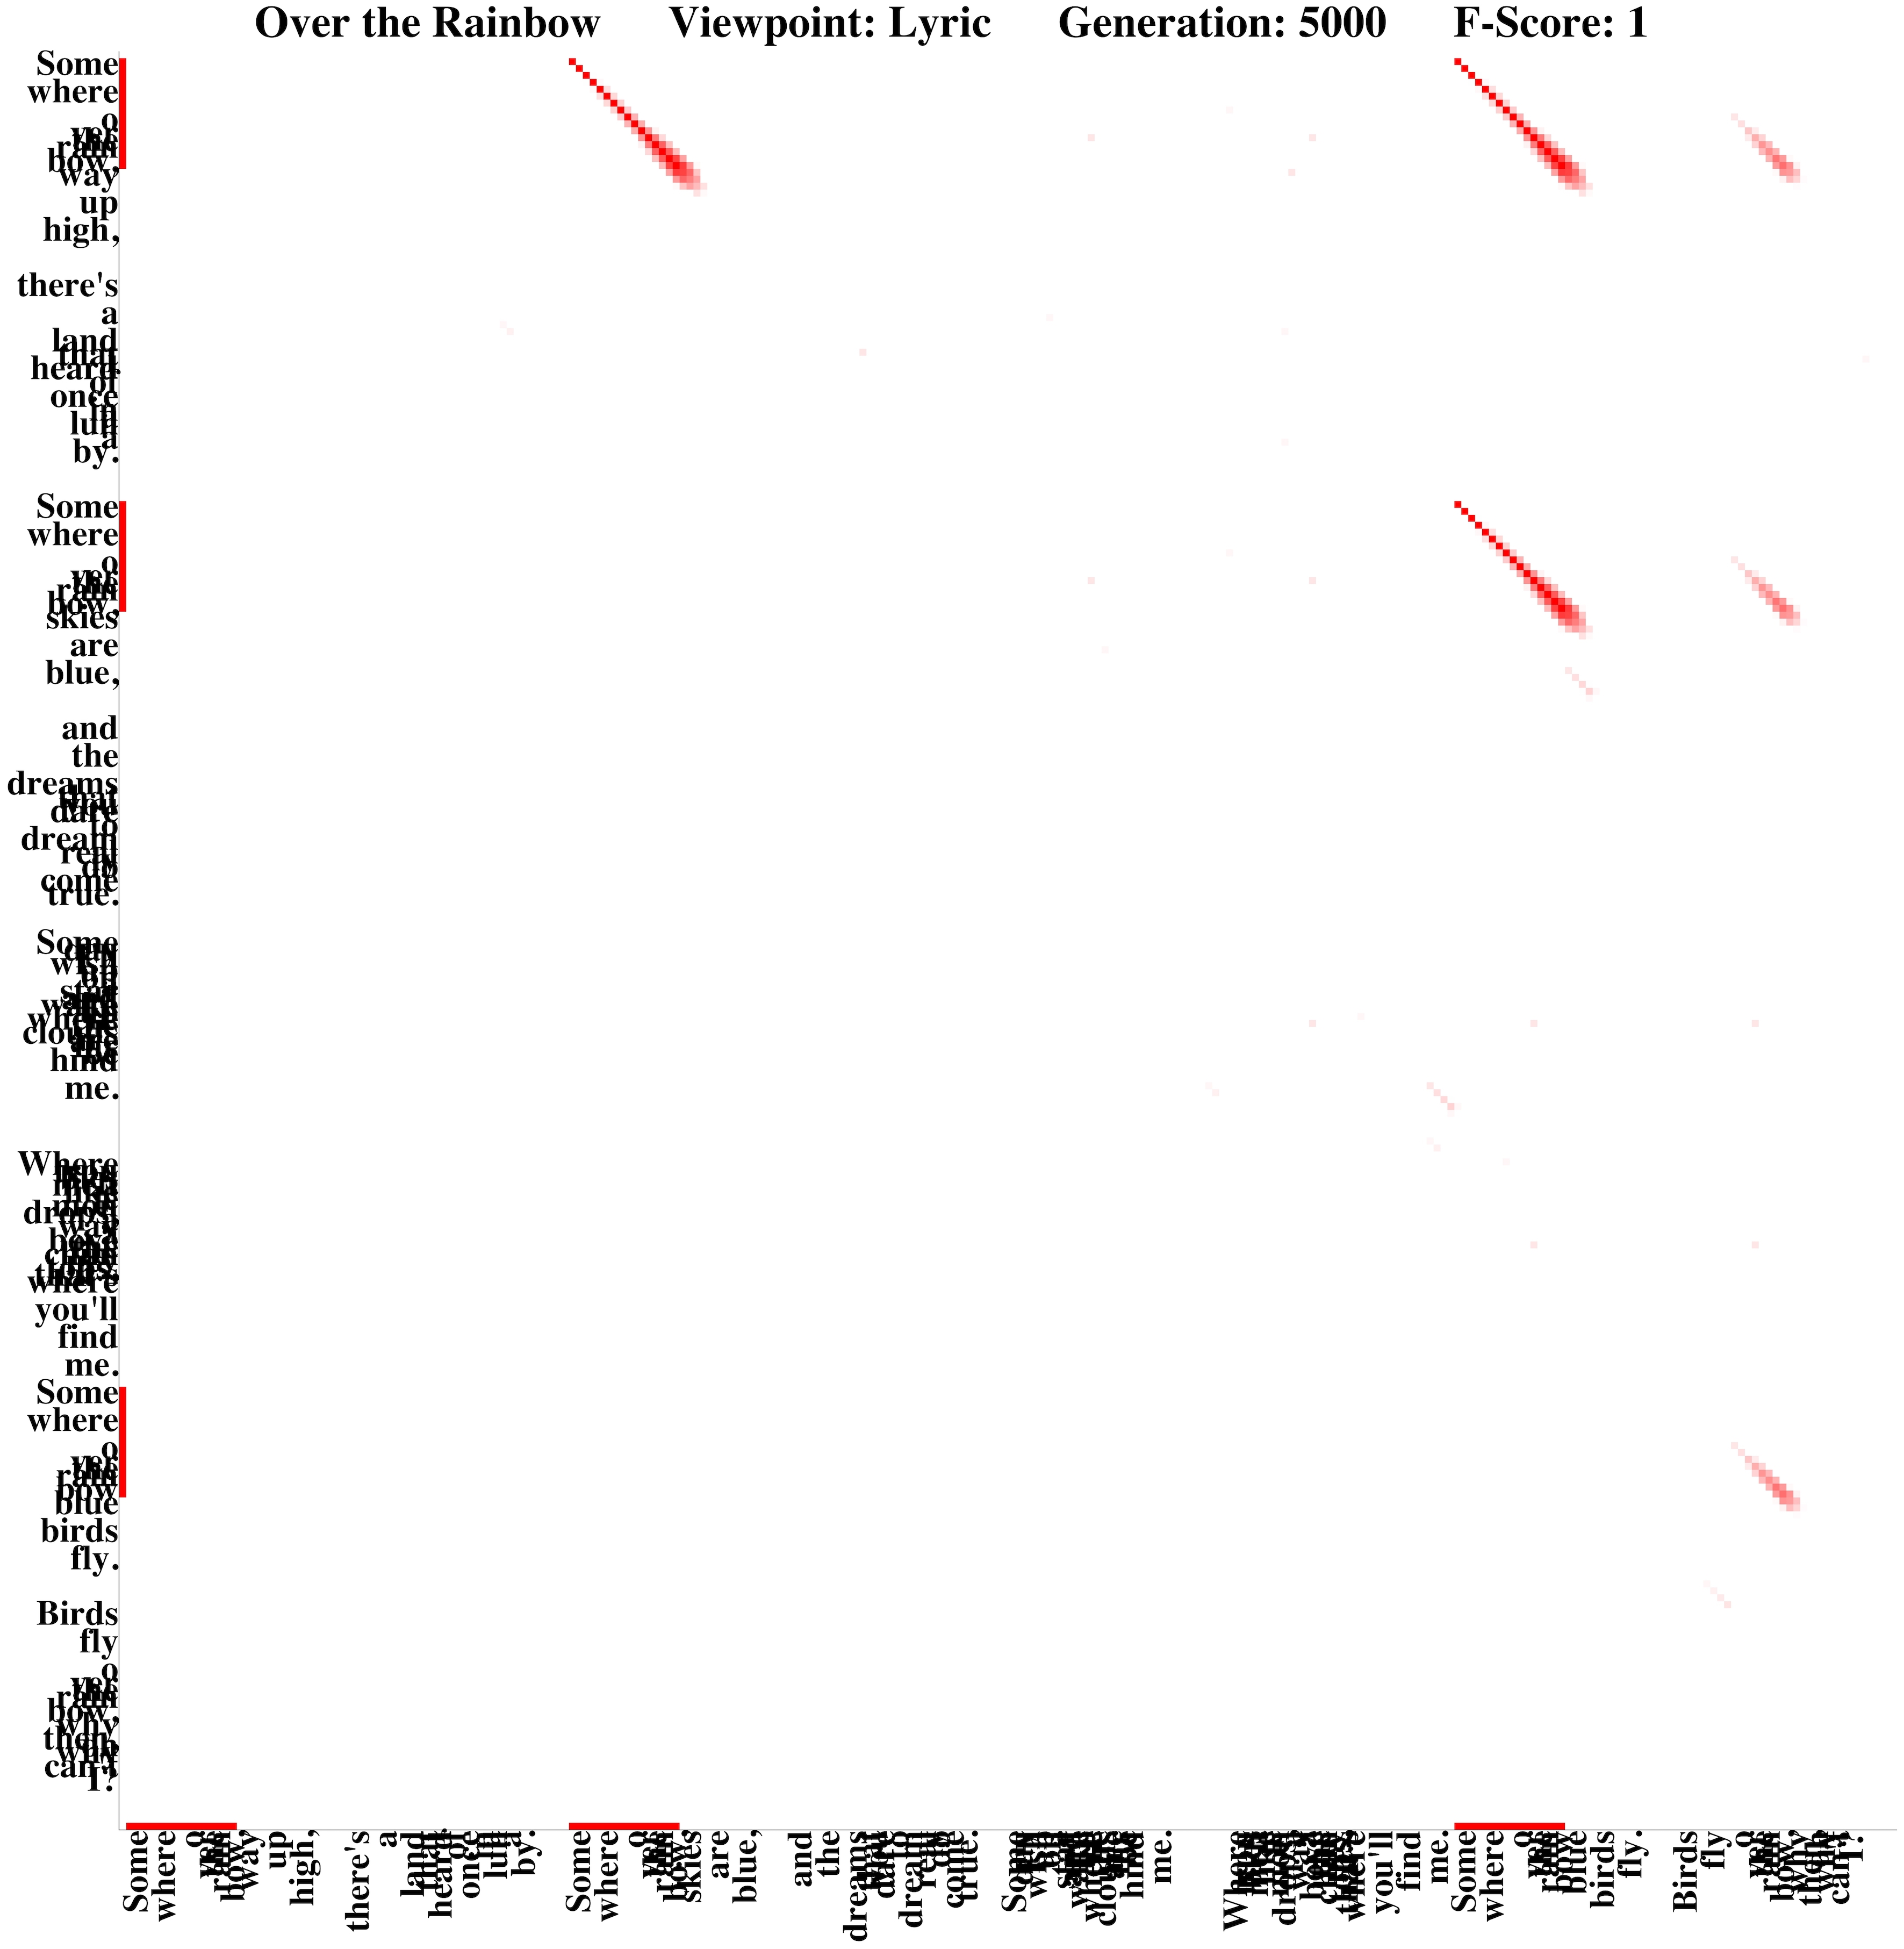
\includegraphics[width=\colwidth]{Over_the_Rainbow_gen5000_id435_lyric} & 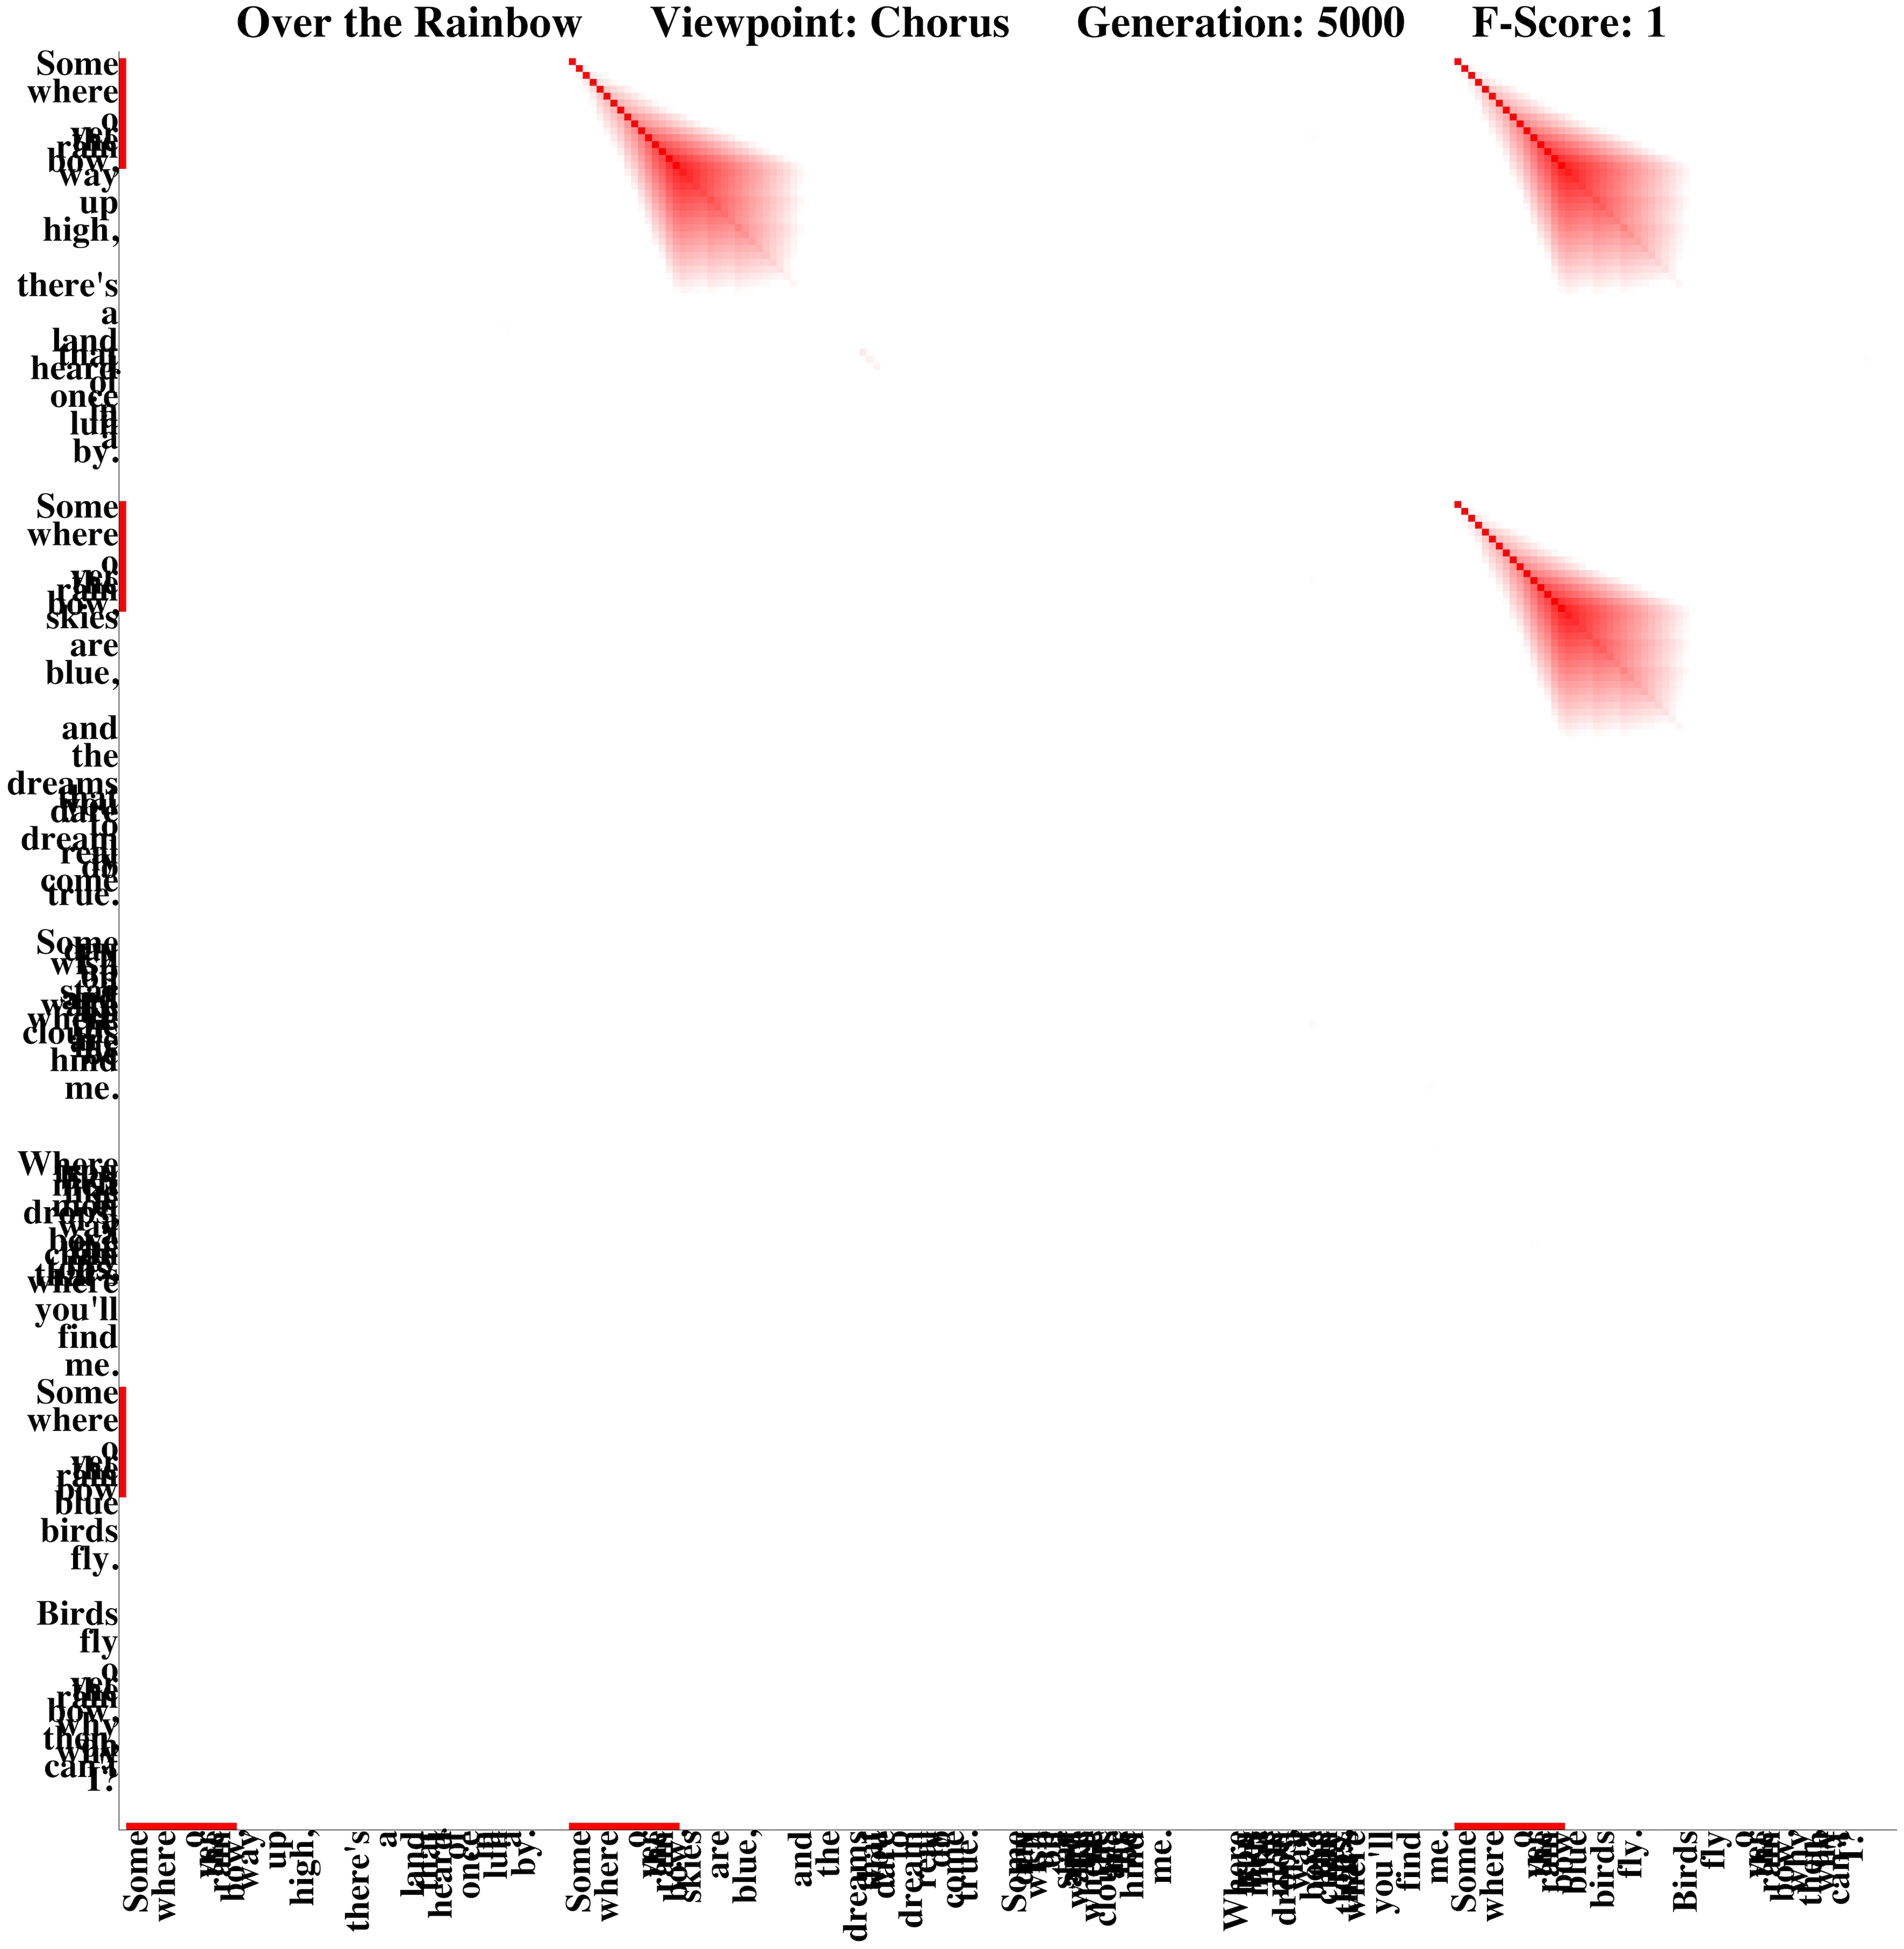
\includegraphics[width=\colwidth]{Over_the_Rainbow_gen5000_id399_chorus} & 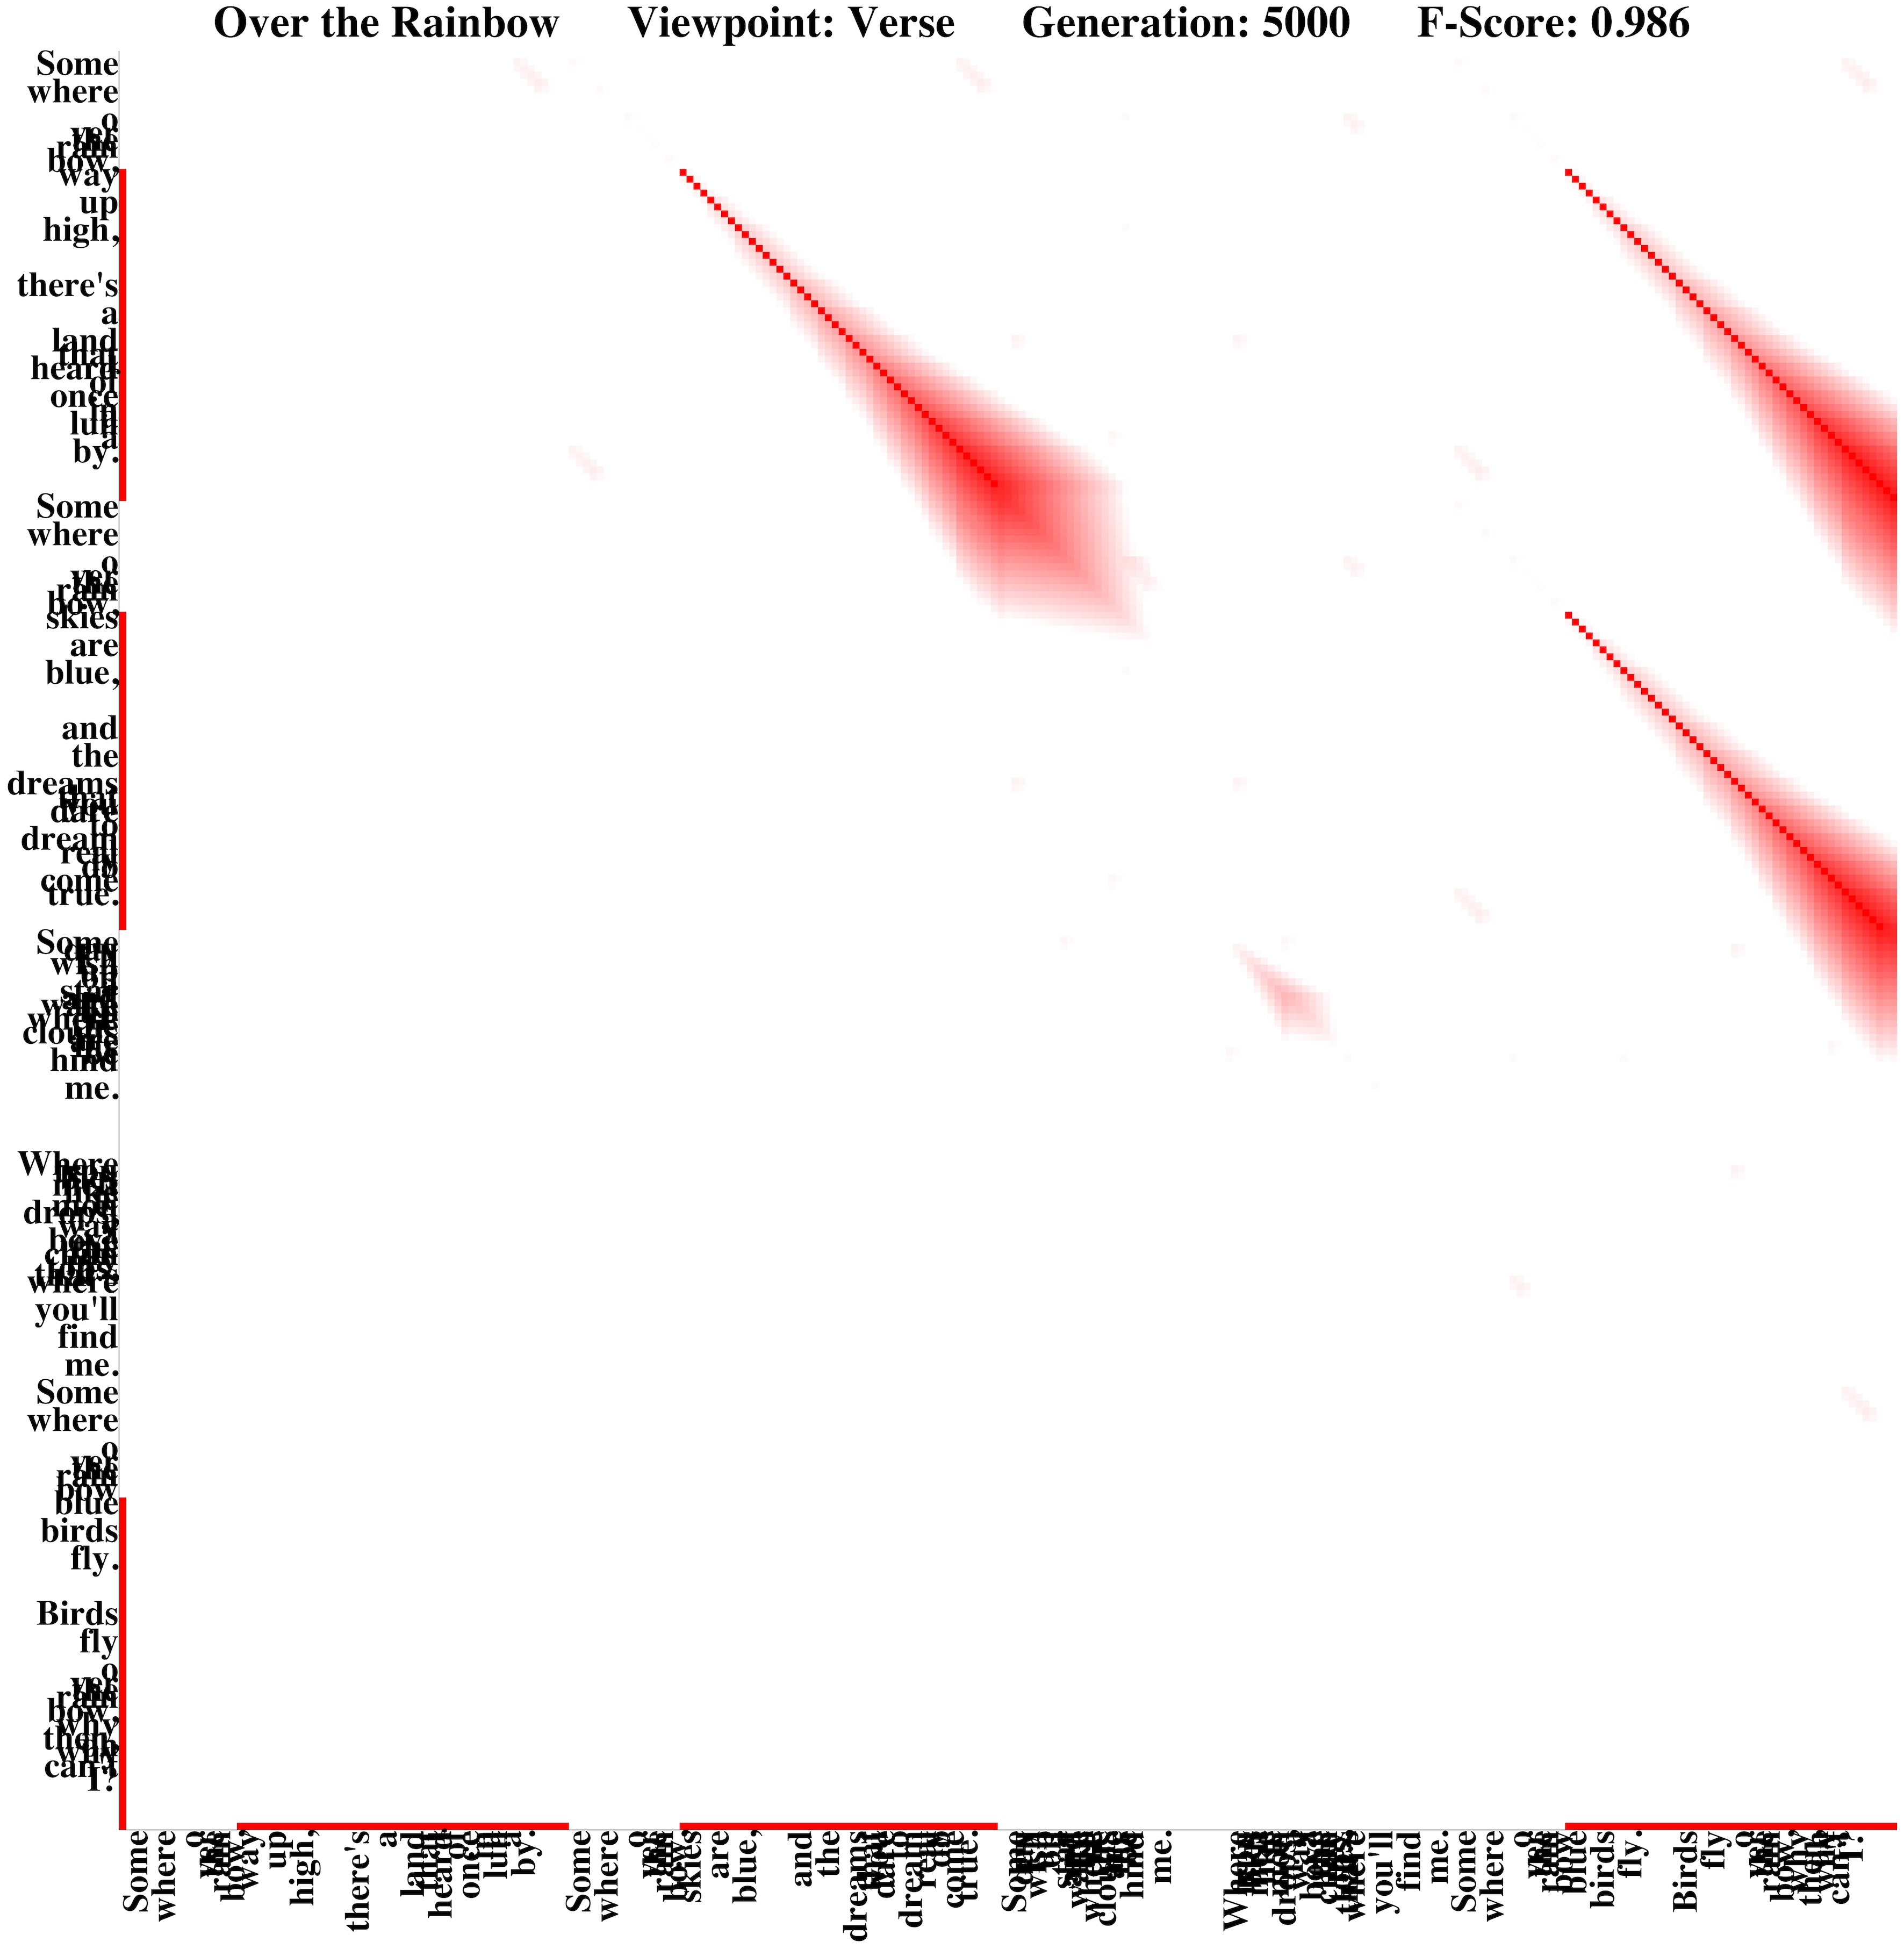
\includegraphics[width=\colwidth]{Over_the_Rainbow_gen5000_id467_verse} \\
% & F-Score:0.87 & F-Score:0.99 & F-Score:0.73 & F-Score:1.00 & F-Score:1.00 & F-Score:0.00 \\
\textbf{Hey Jude} $F_{1}=0.66$ & 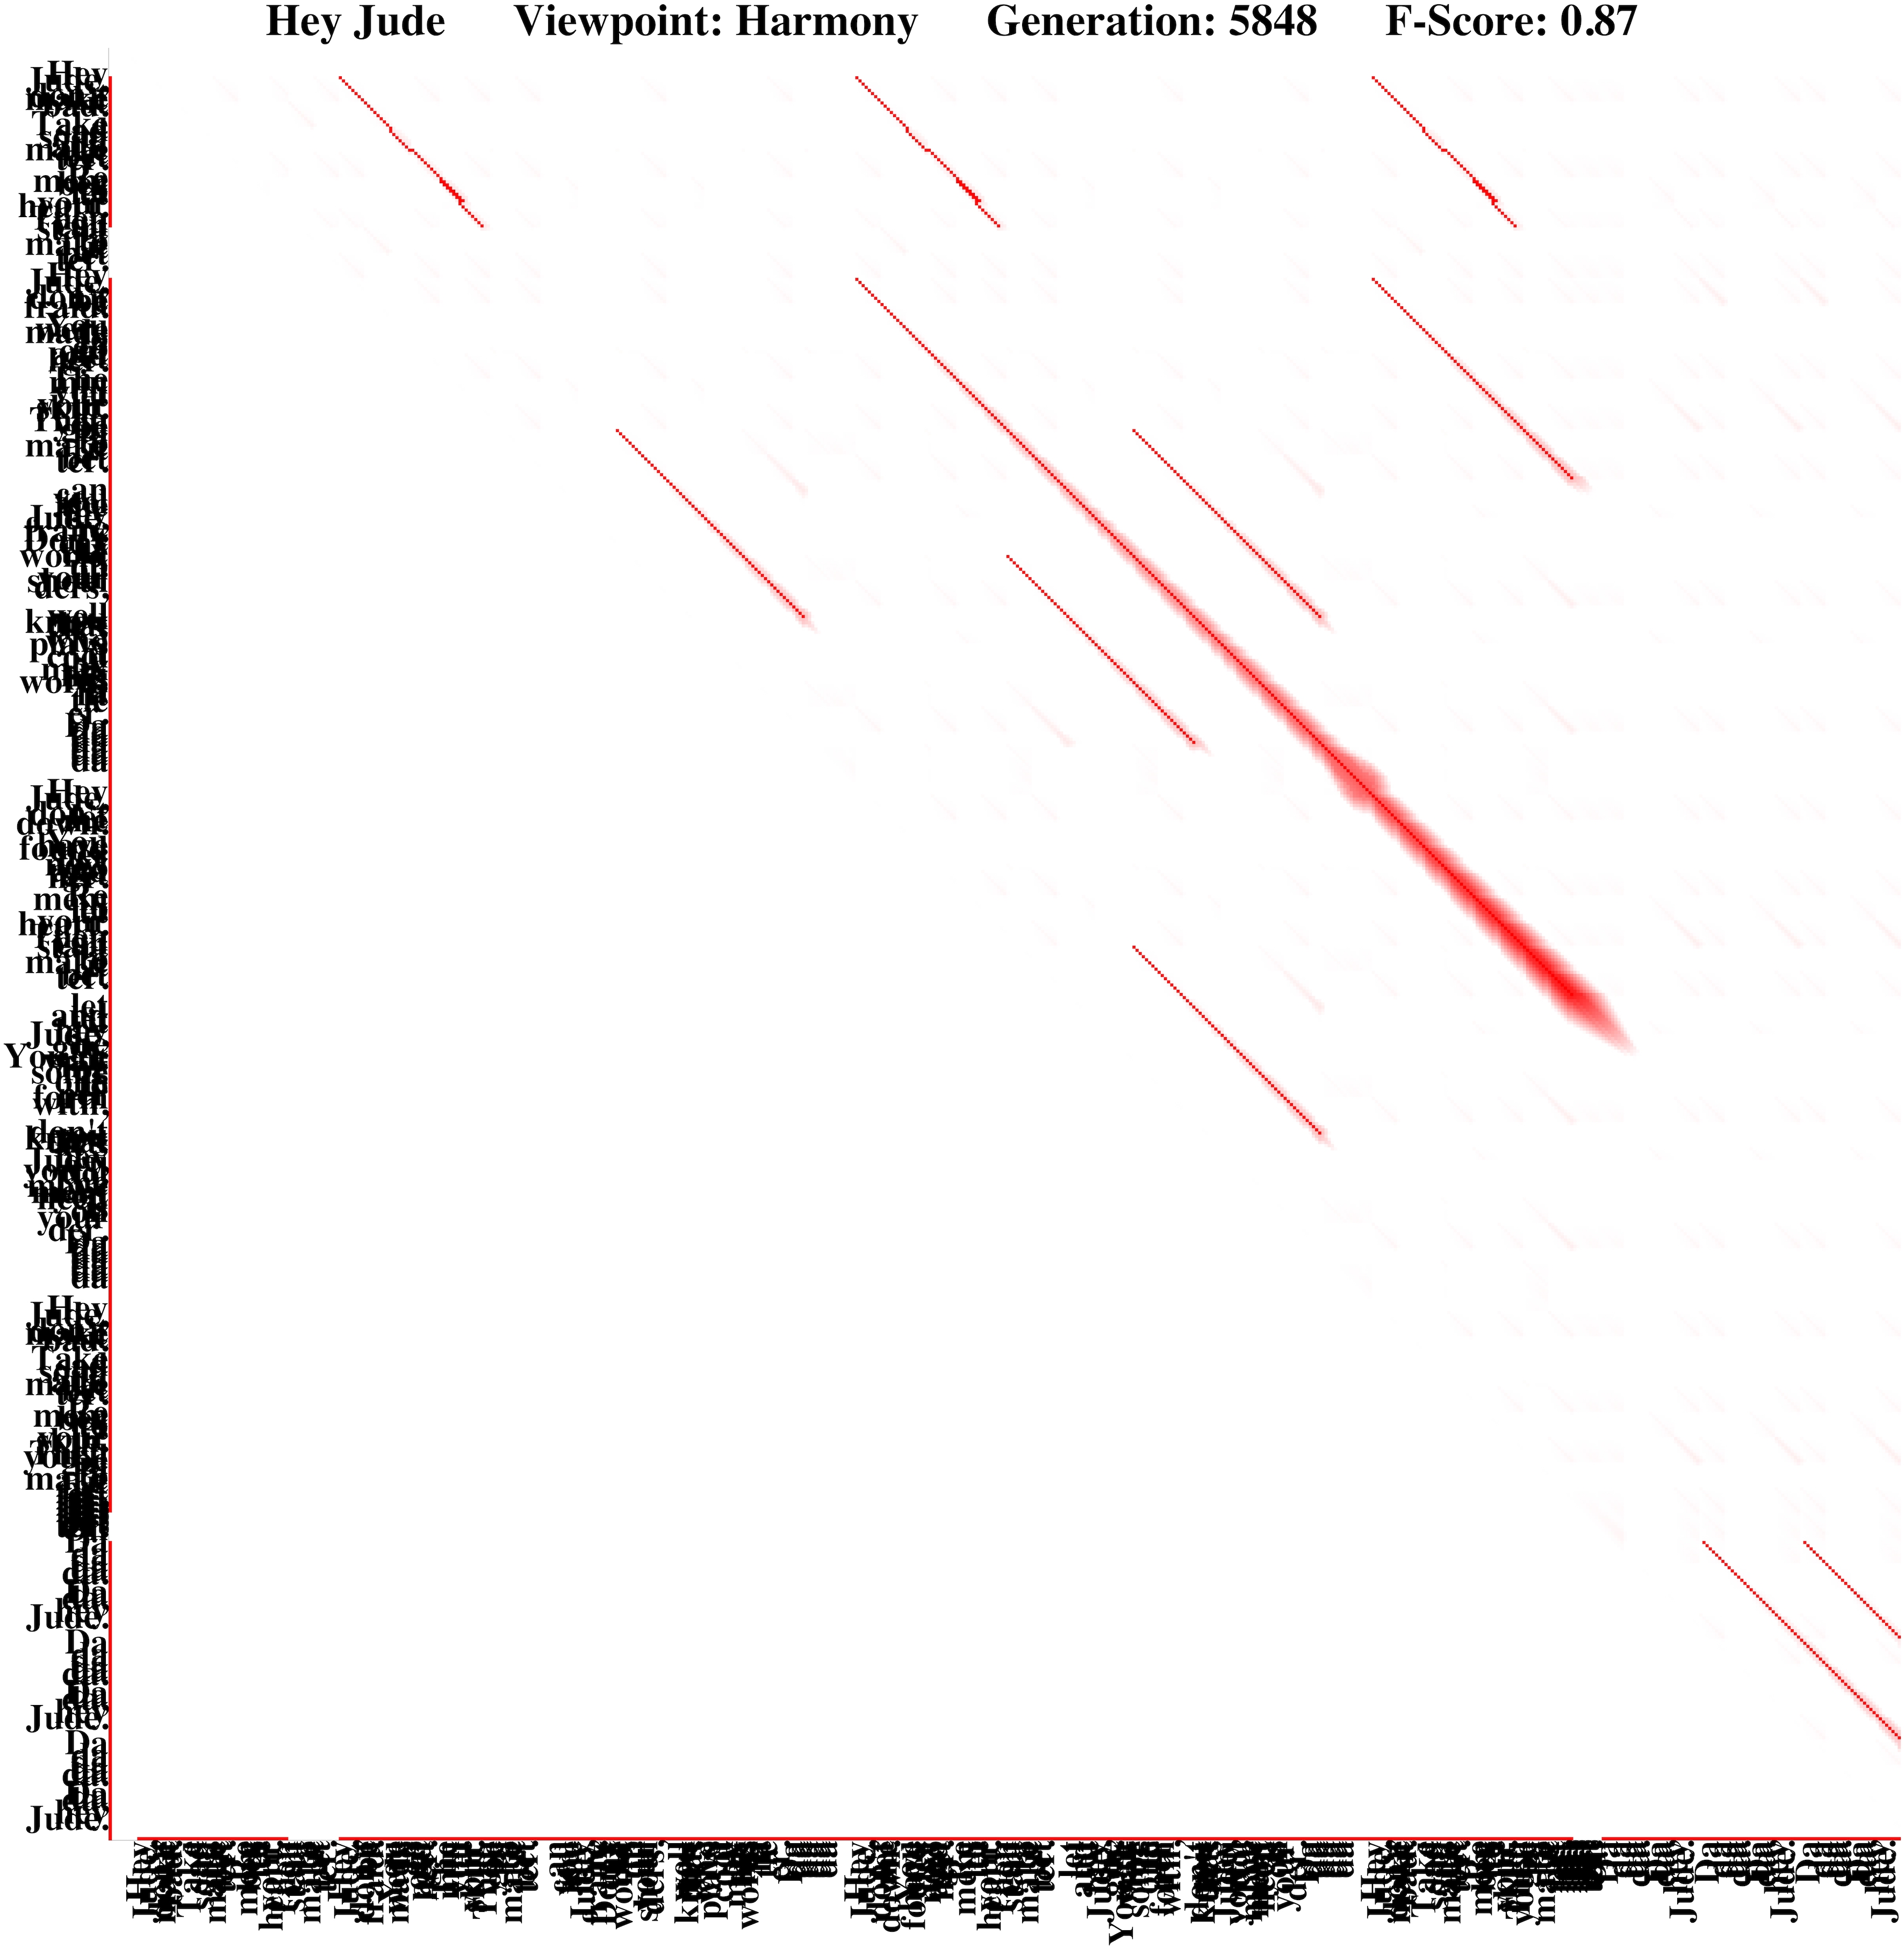
\includegraphics[width=\colwidth]{Hey_Jude_gen5848_id631_harmony} & 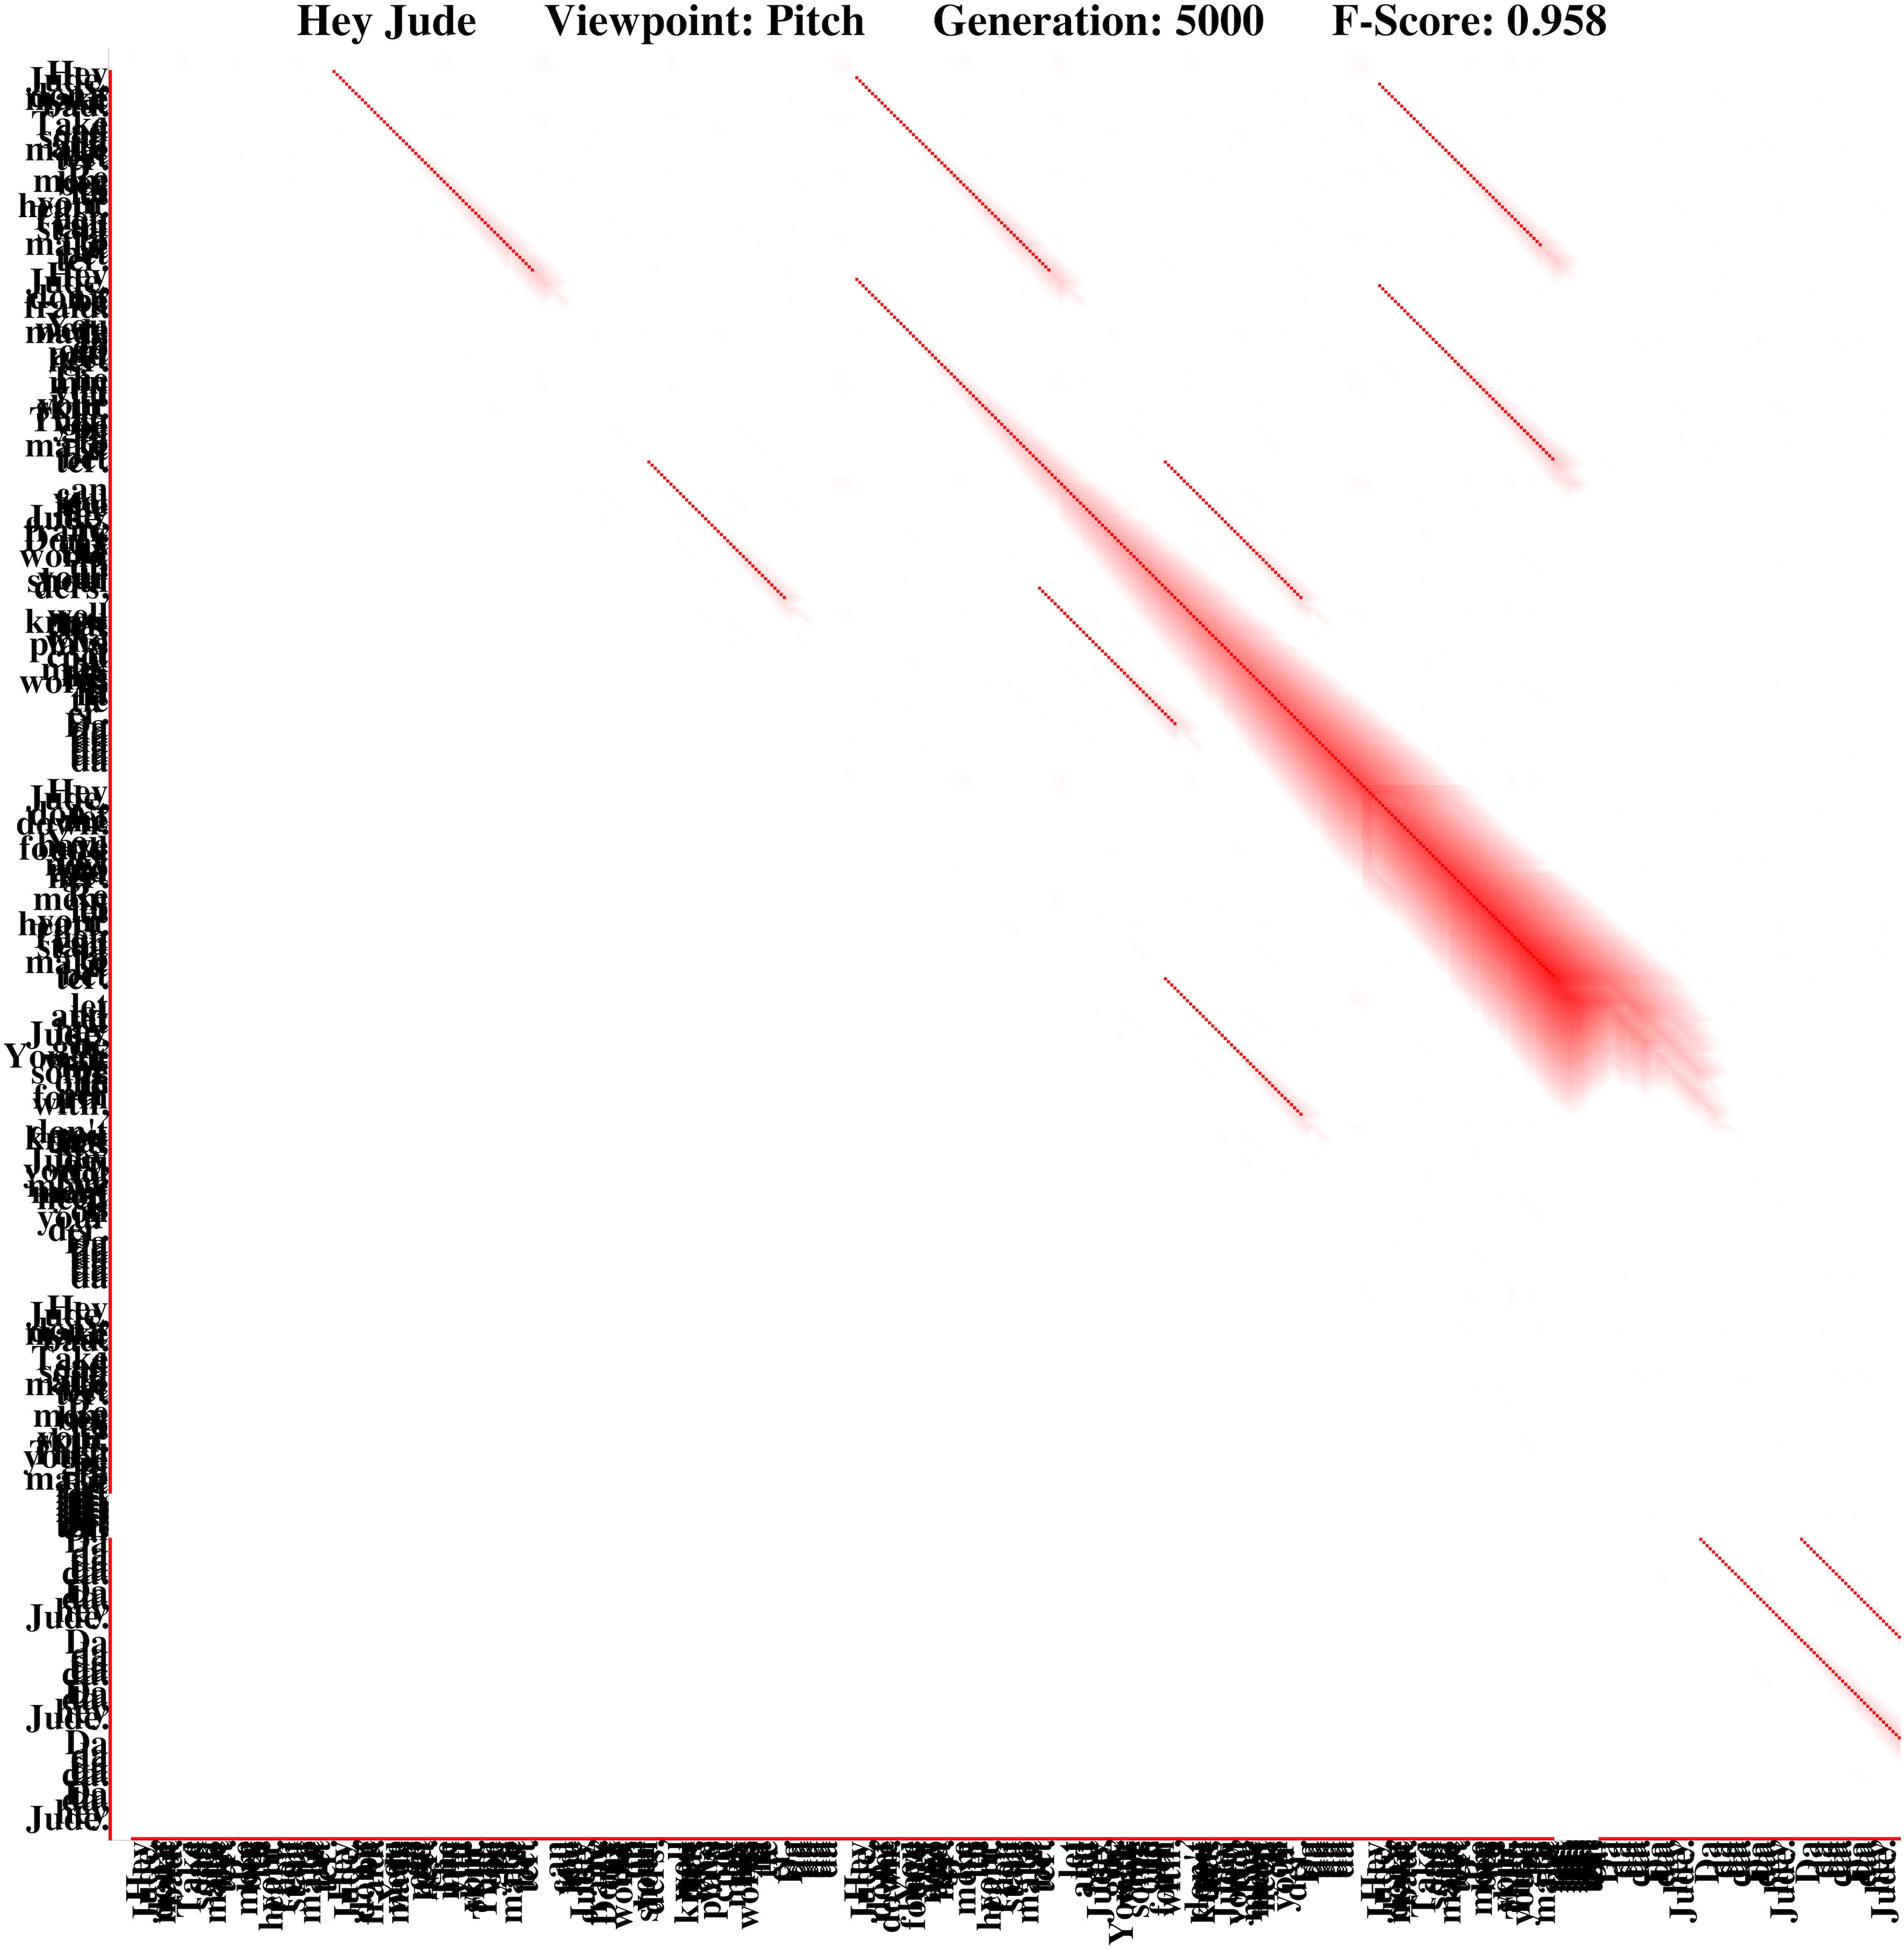
\includegraphics[width=\colwidth]{Hey_Jude_gen5000_id544_pitch} & 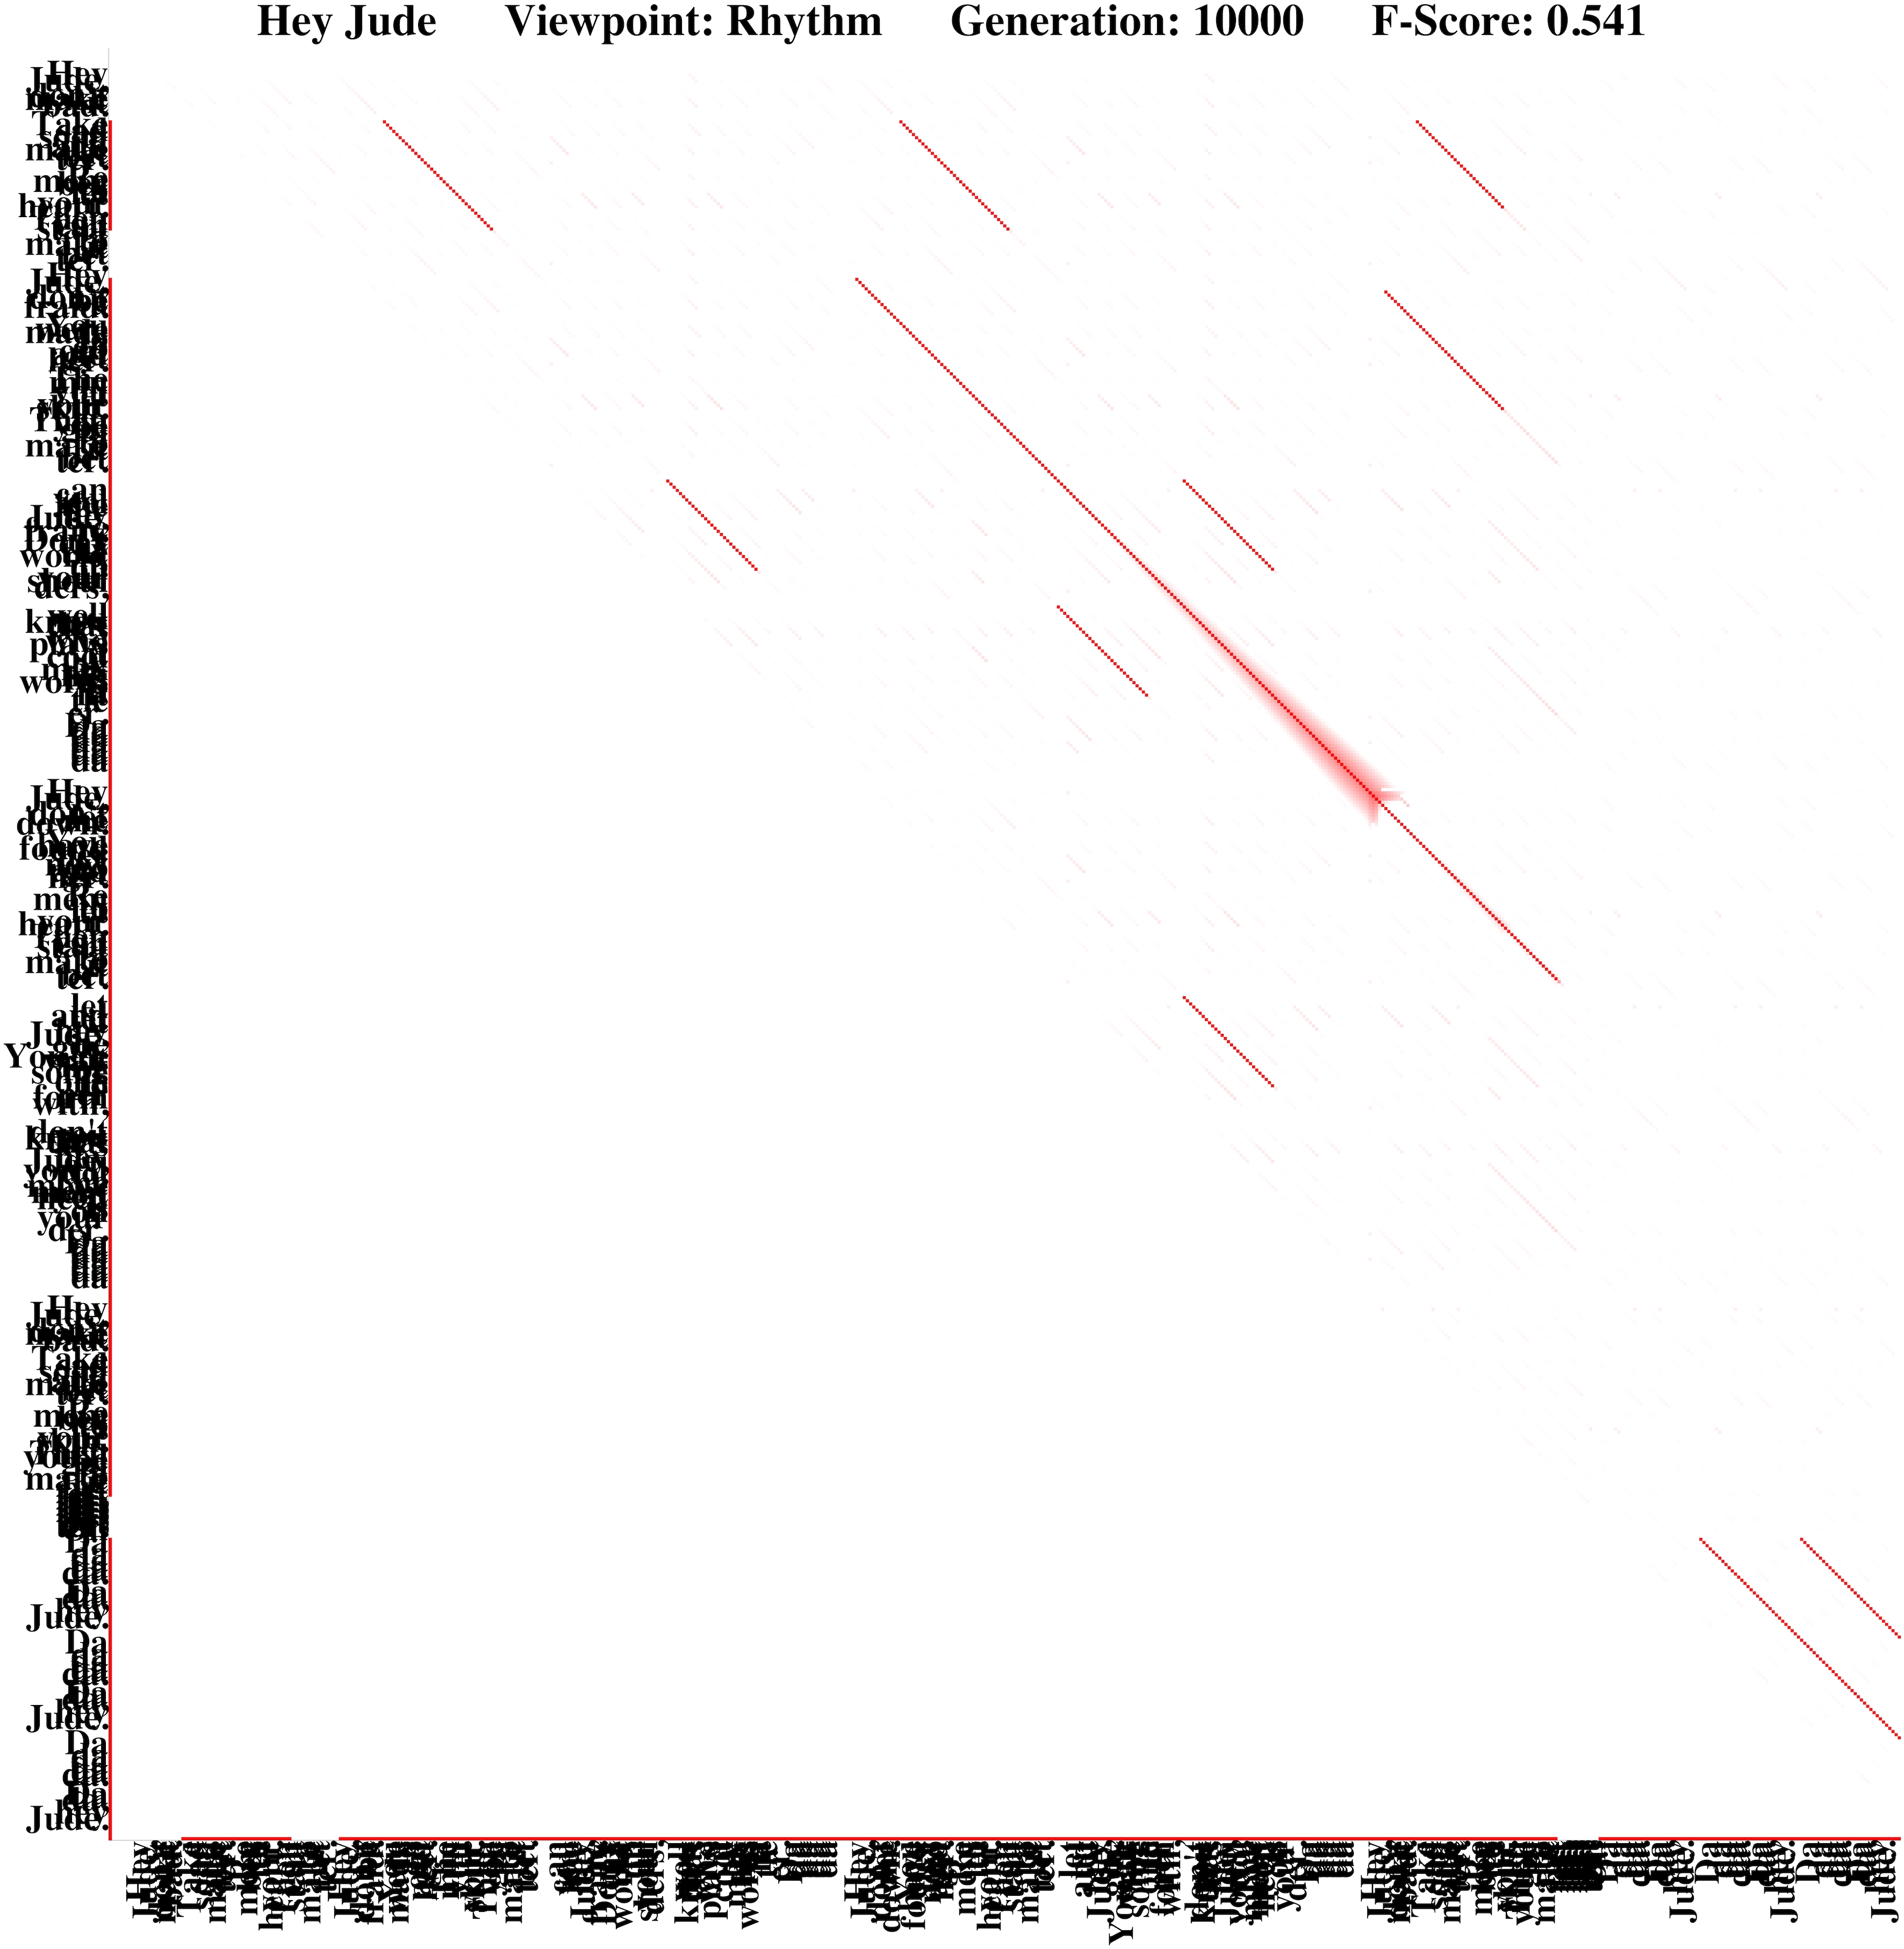
\includegraphics[width=\colwidth]{Hey_Jude_gen10000_id784_rhythm} & 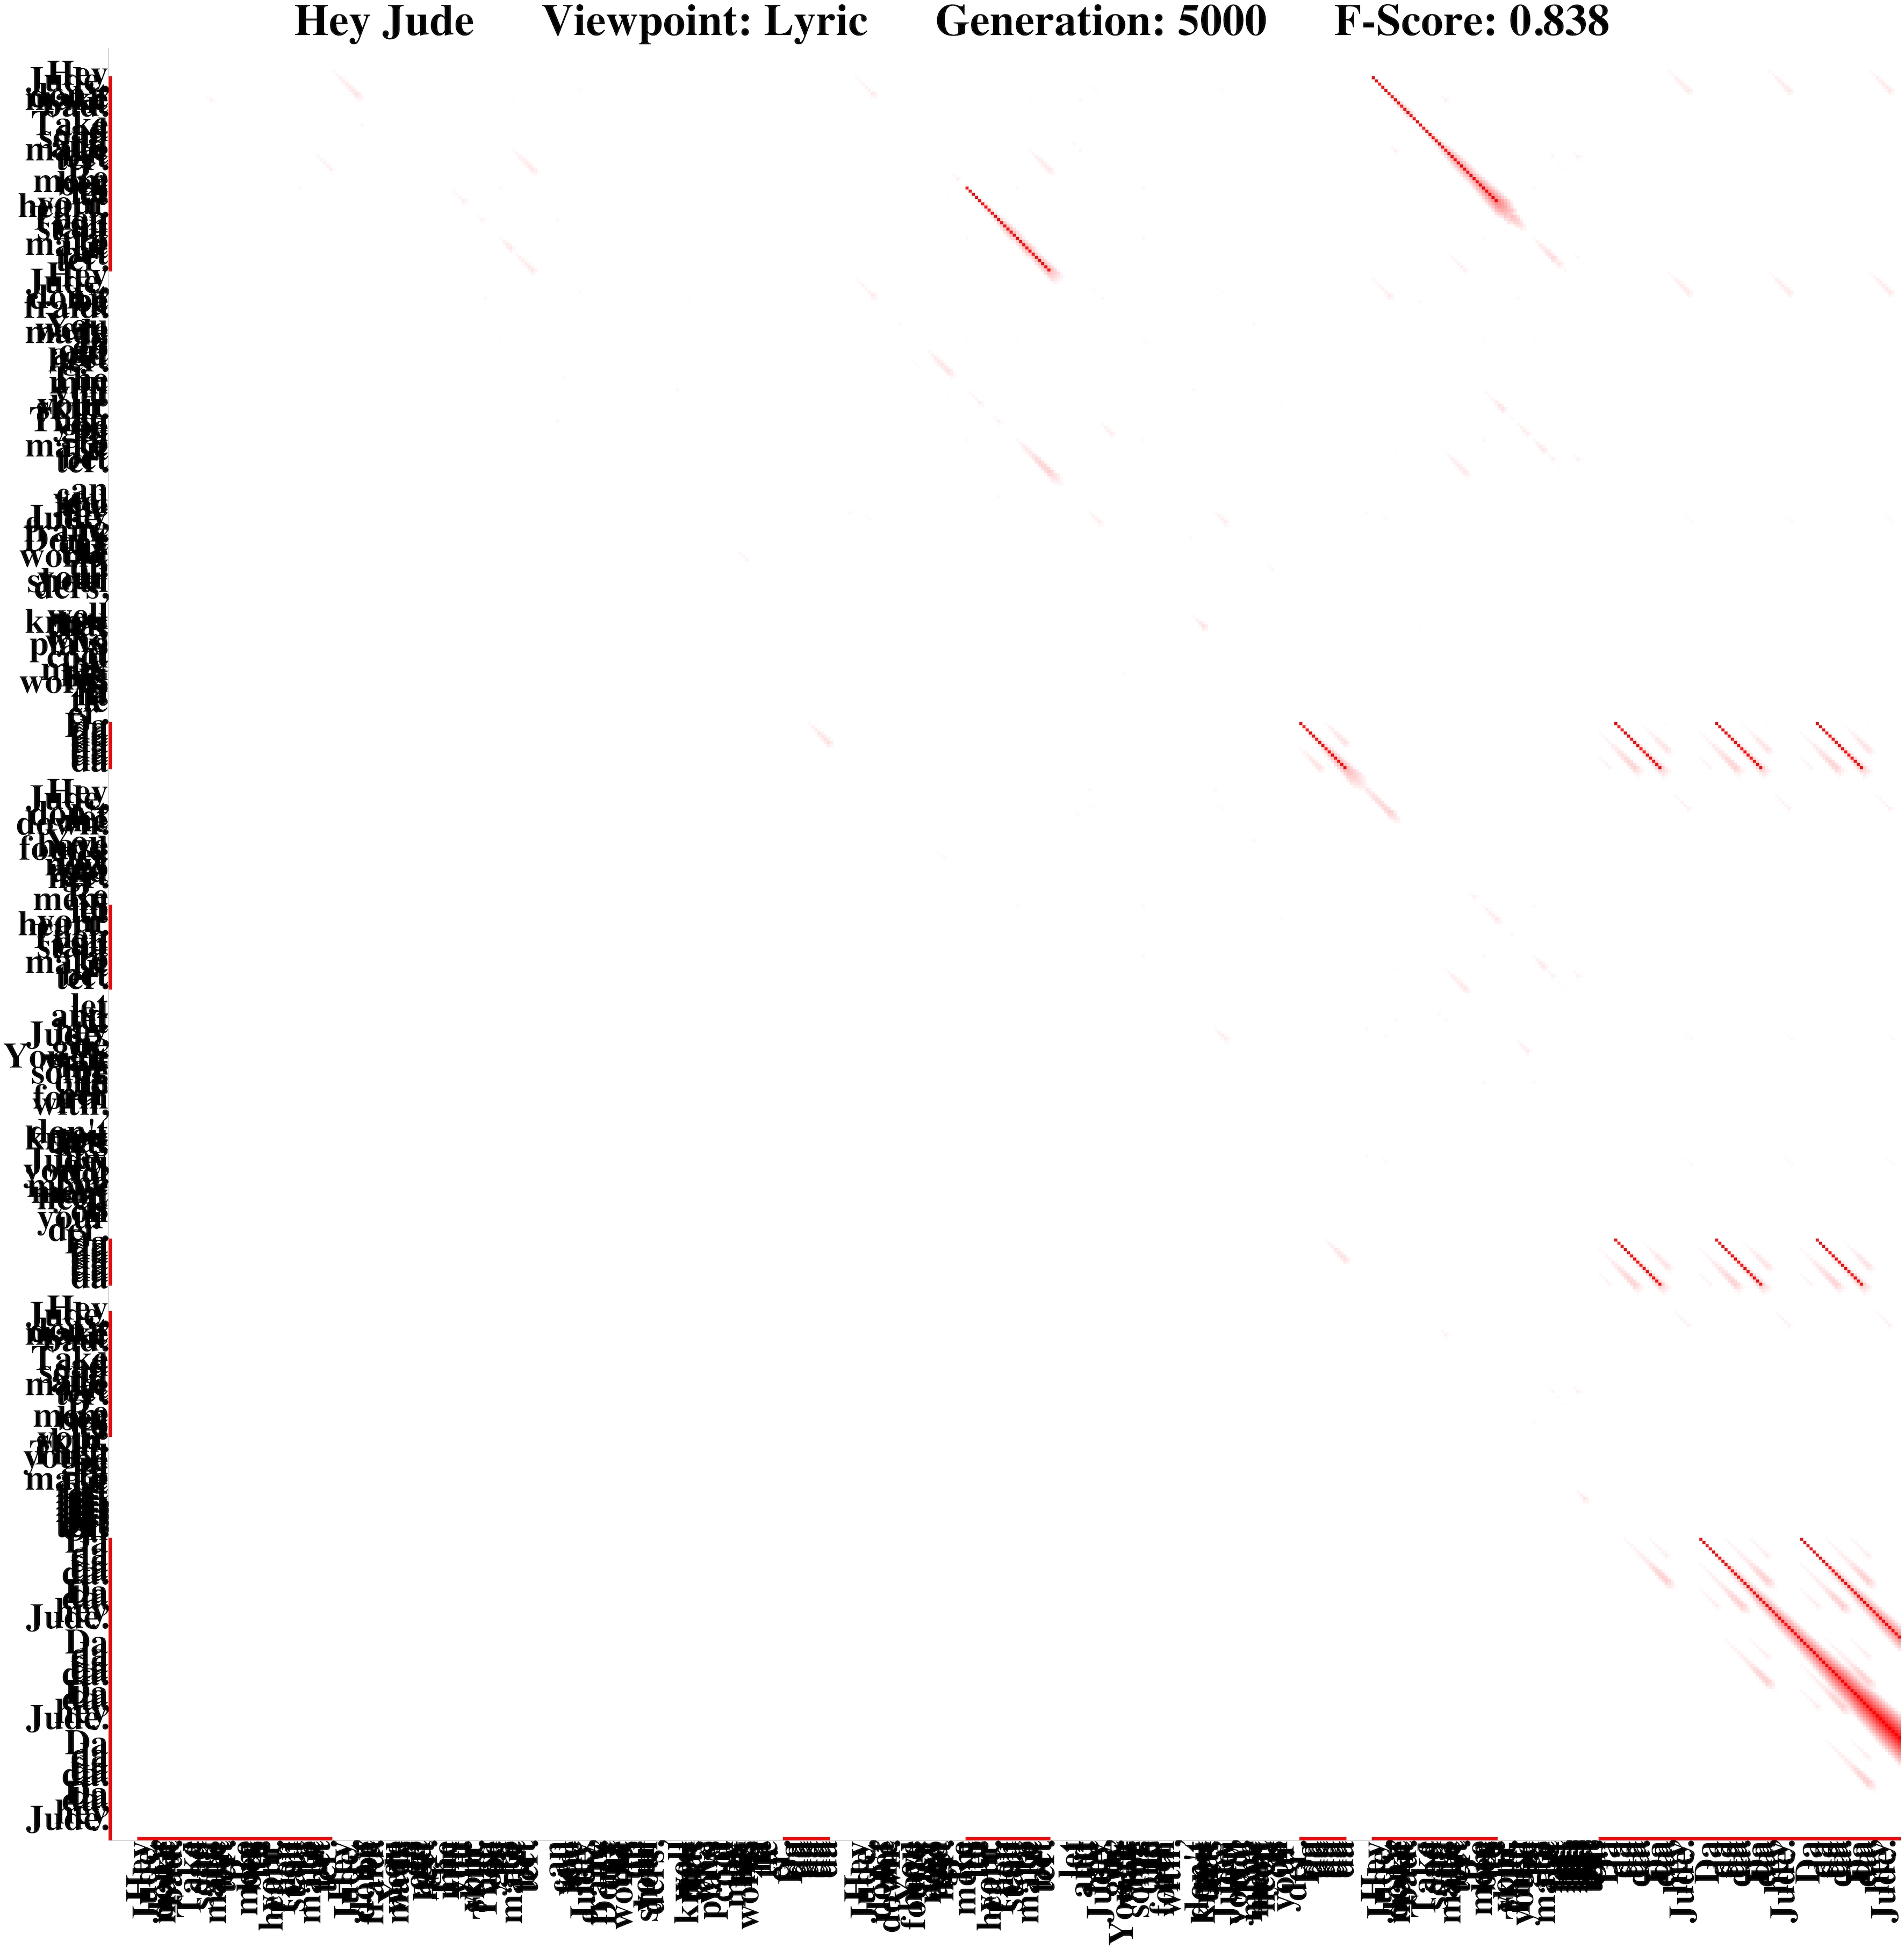
\includegraphics[width=\colwidth]{Hey_Jude_gen5000_id435_lyric} & 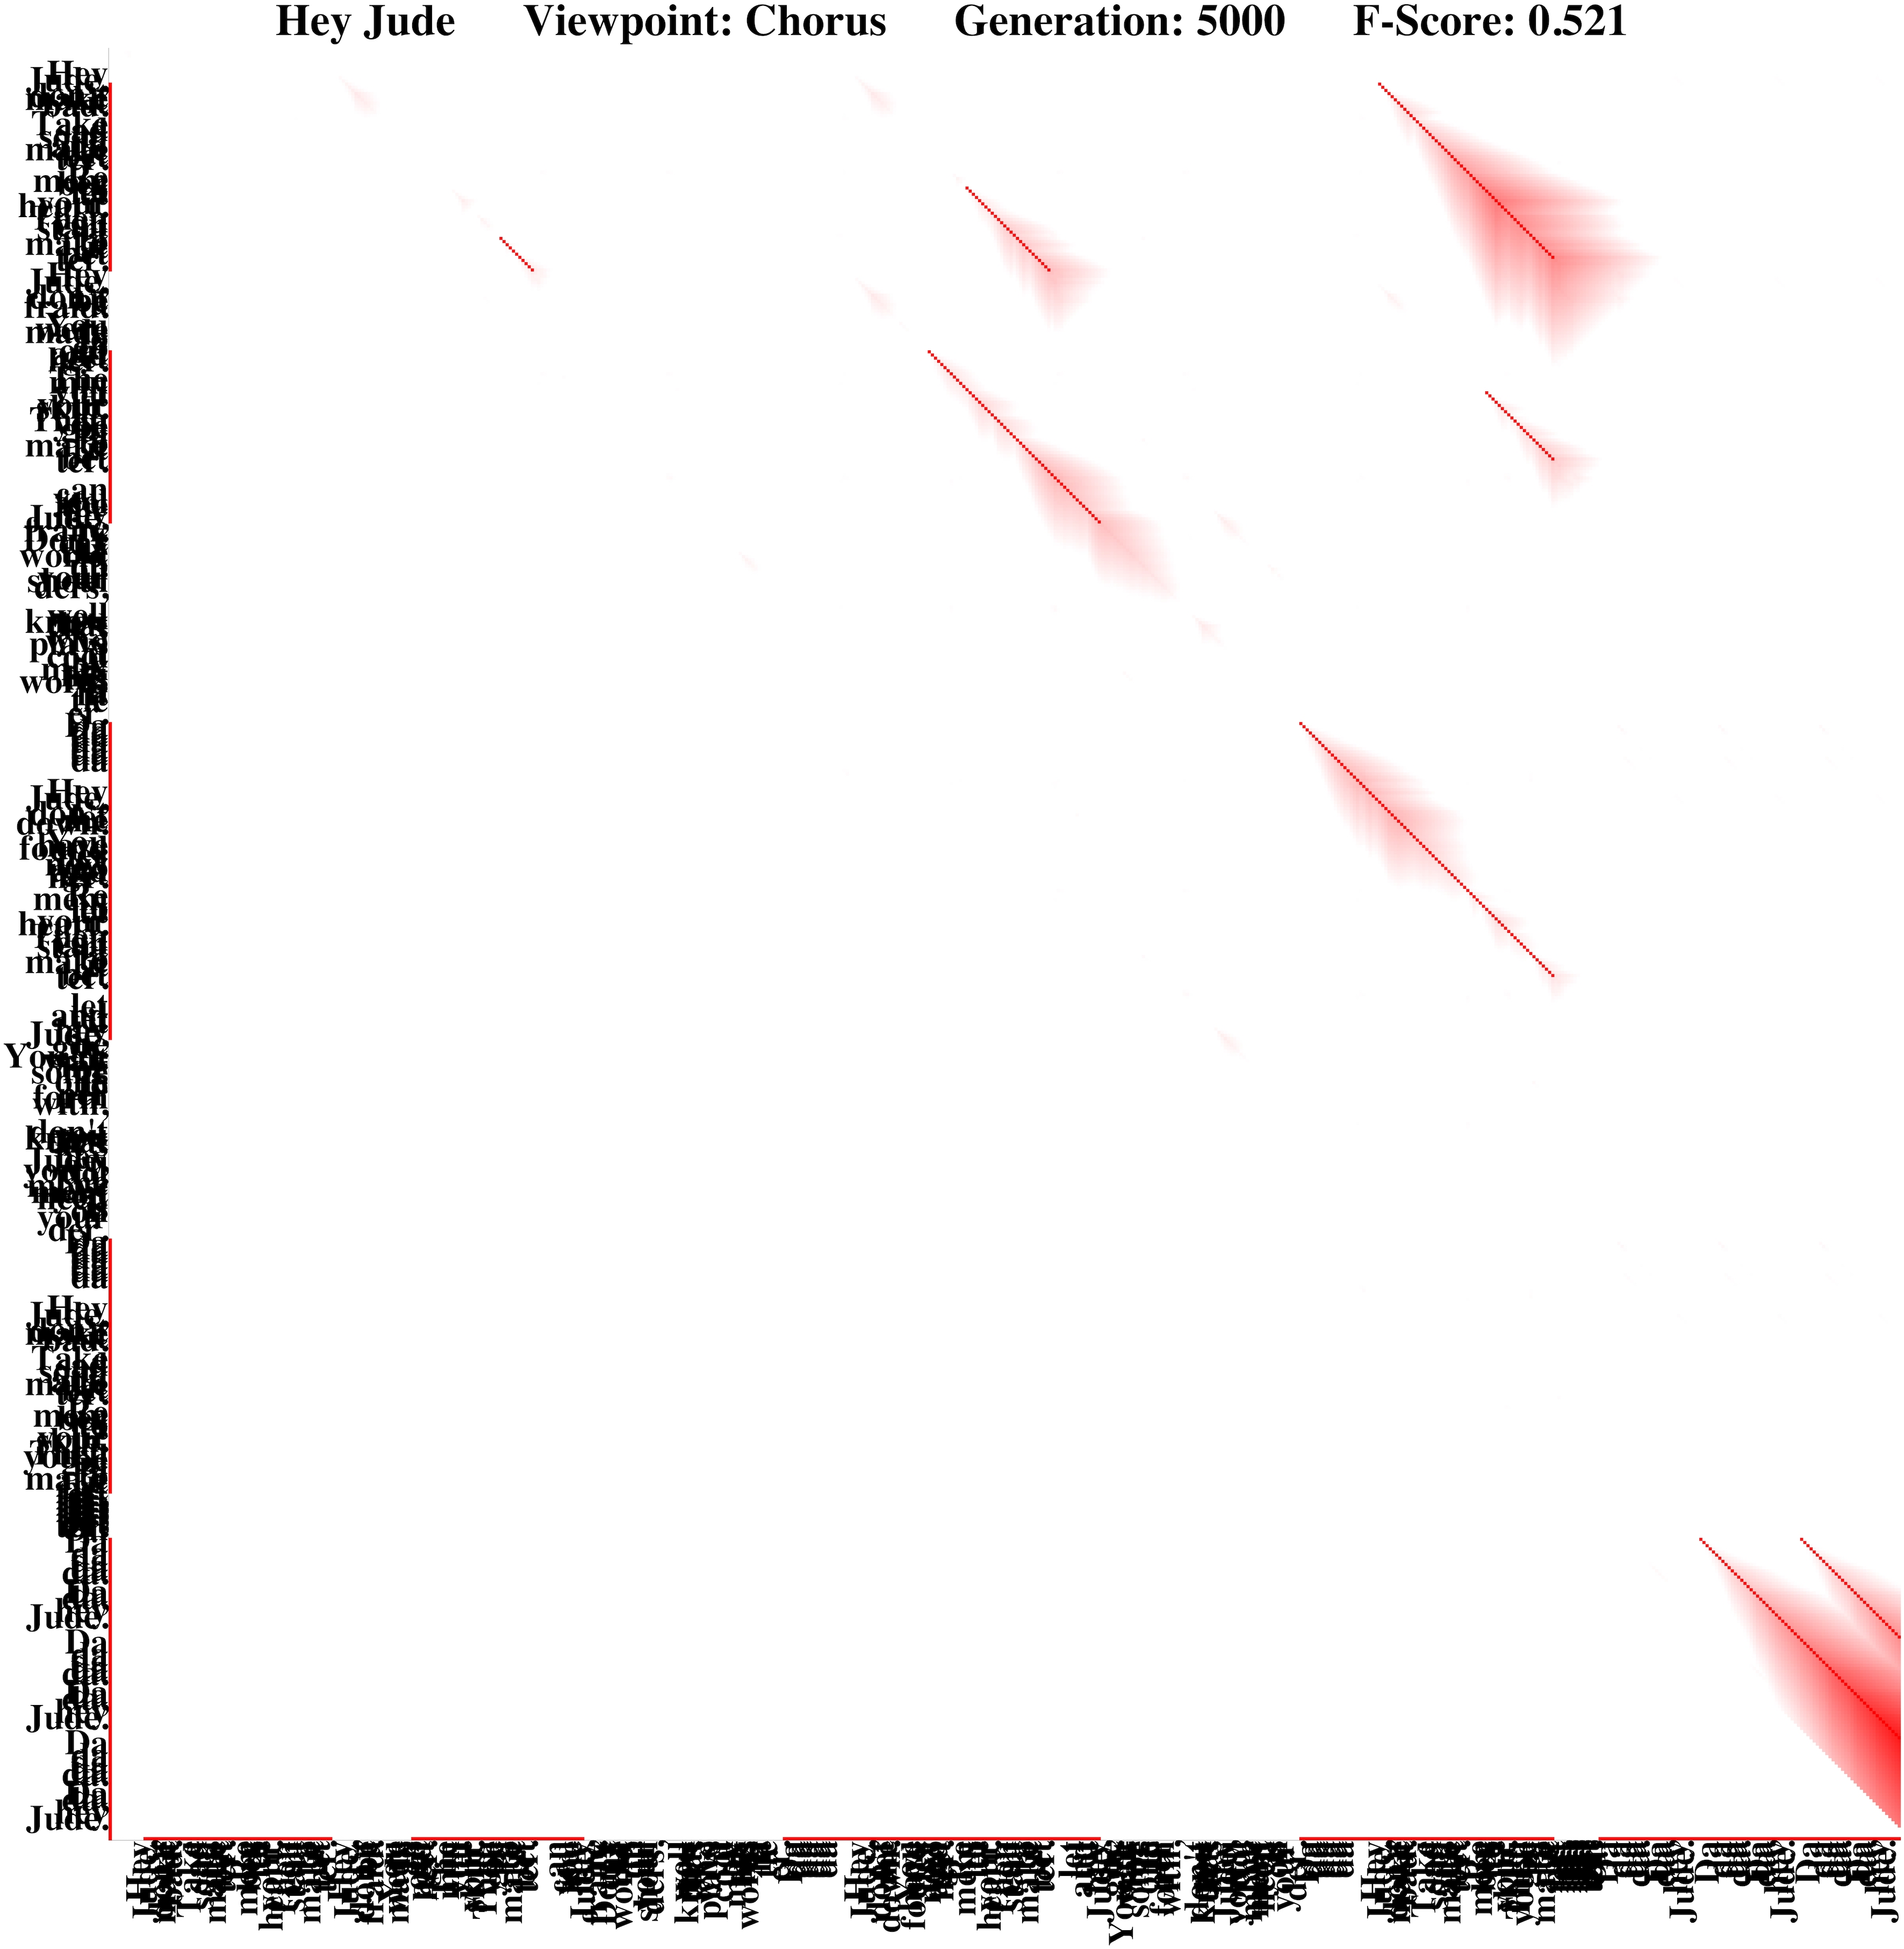
\includegraphics[width=\colwidth]{Hey_Jude_gen5000_id399_chorus} & 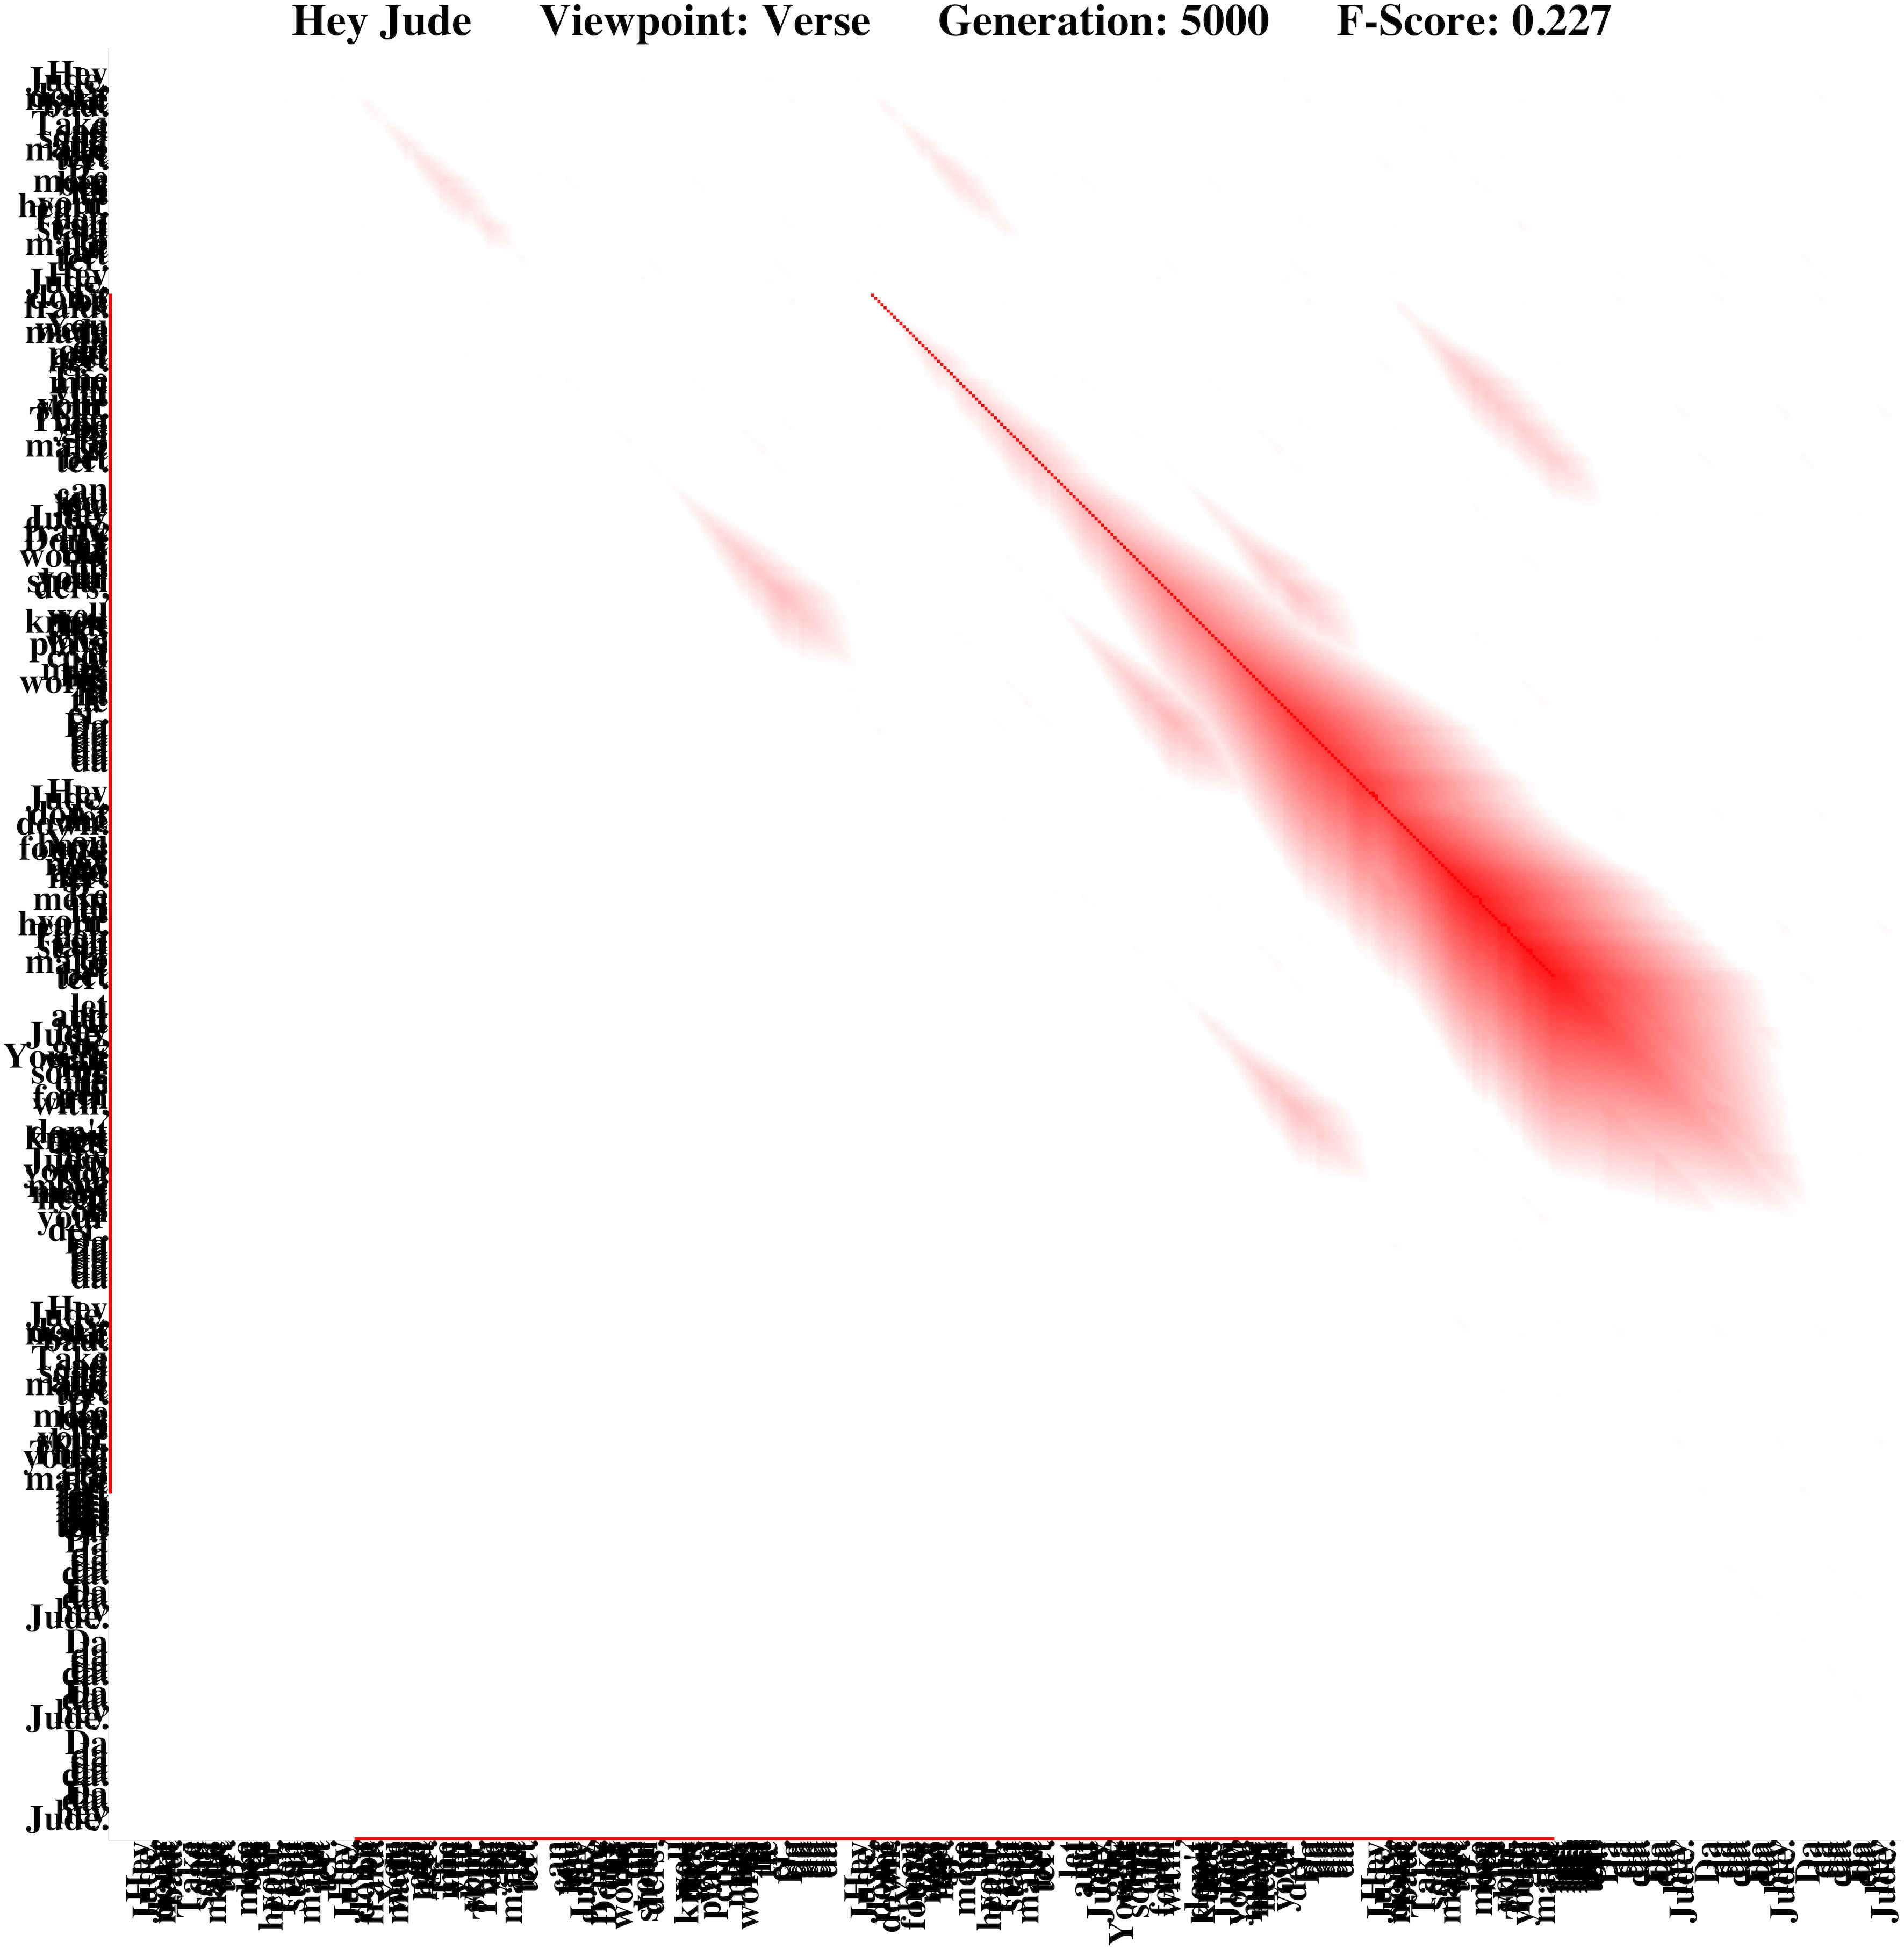
\includegraphics[width=\colwidth]{Hey_Jude_gen5000_id467_verse} \\
% & F-Score:0.87 & F-Score:0.98 & F-Score:0.87 & F-Score:0.87 & F-Score:0.78 & F-Score:0.00 \\
\textbf{Take Me Home, Country Roads} $F_{1}=0.87$ & 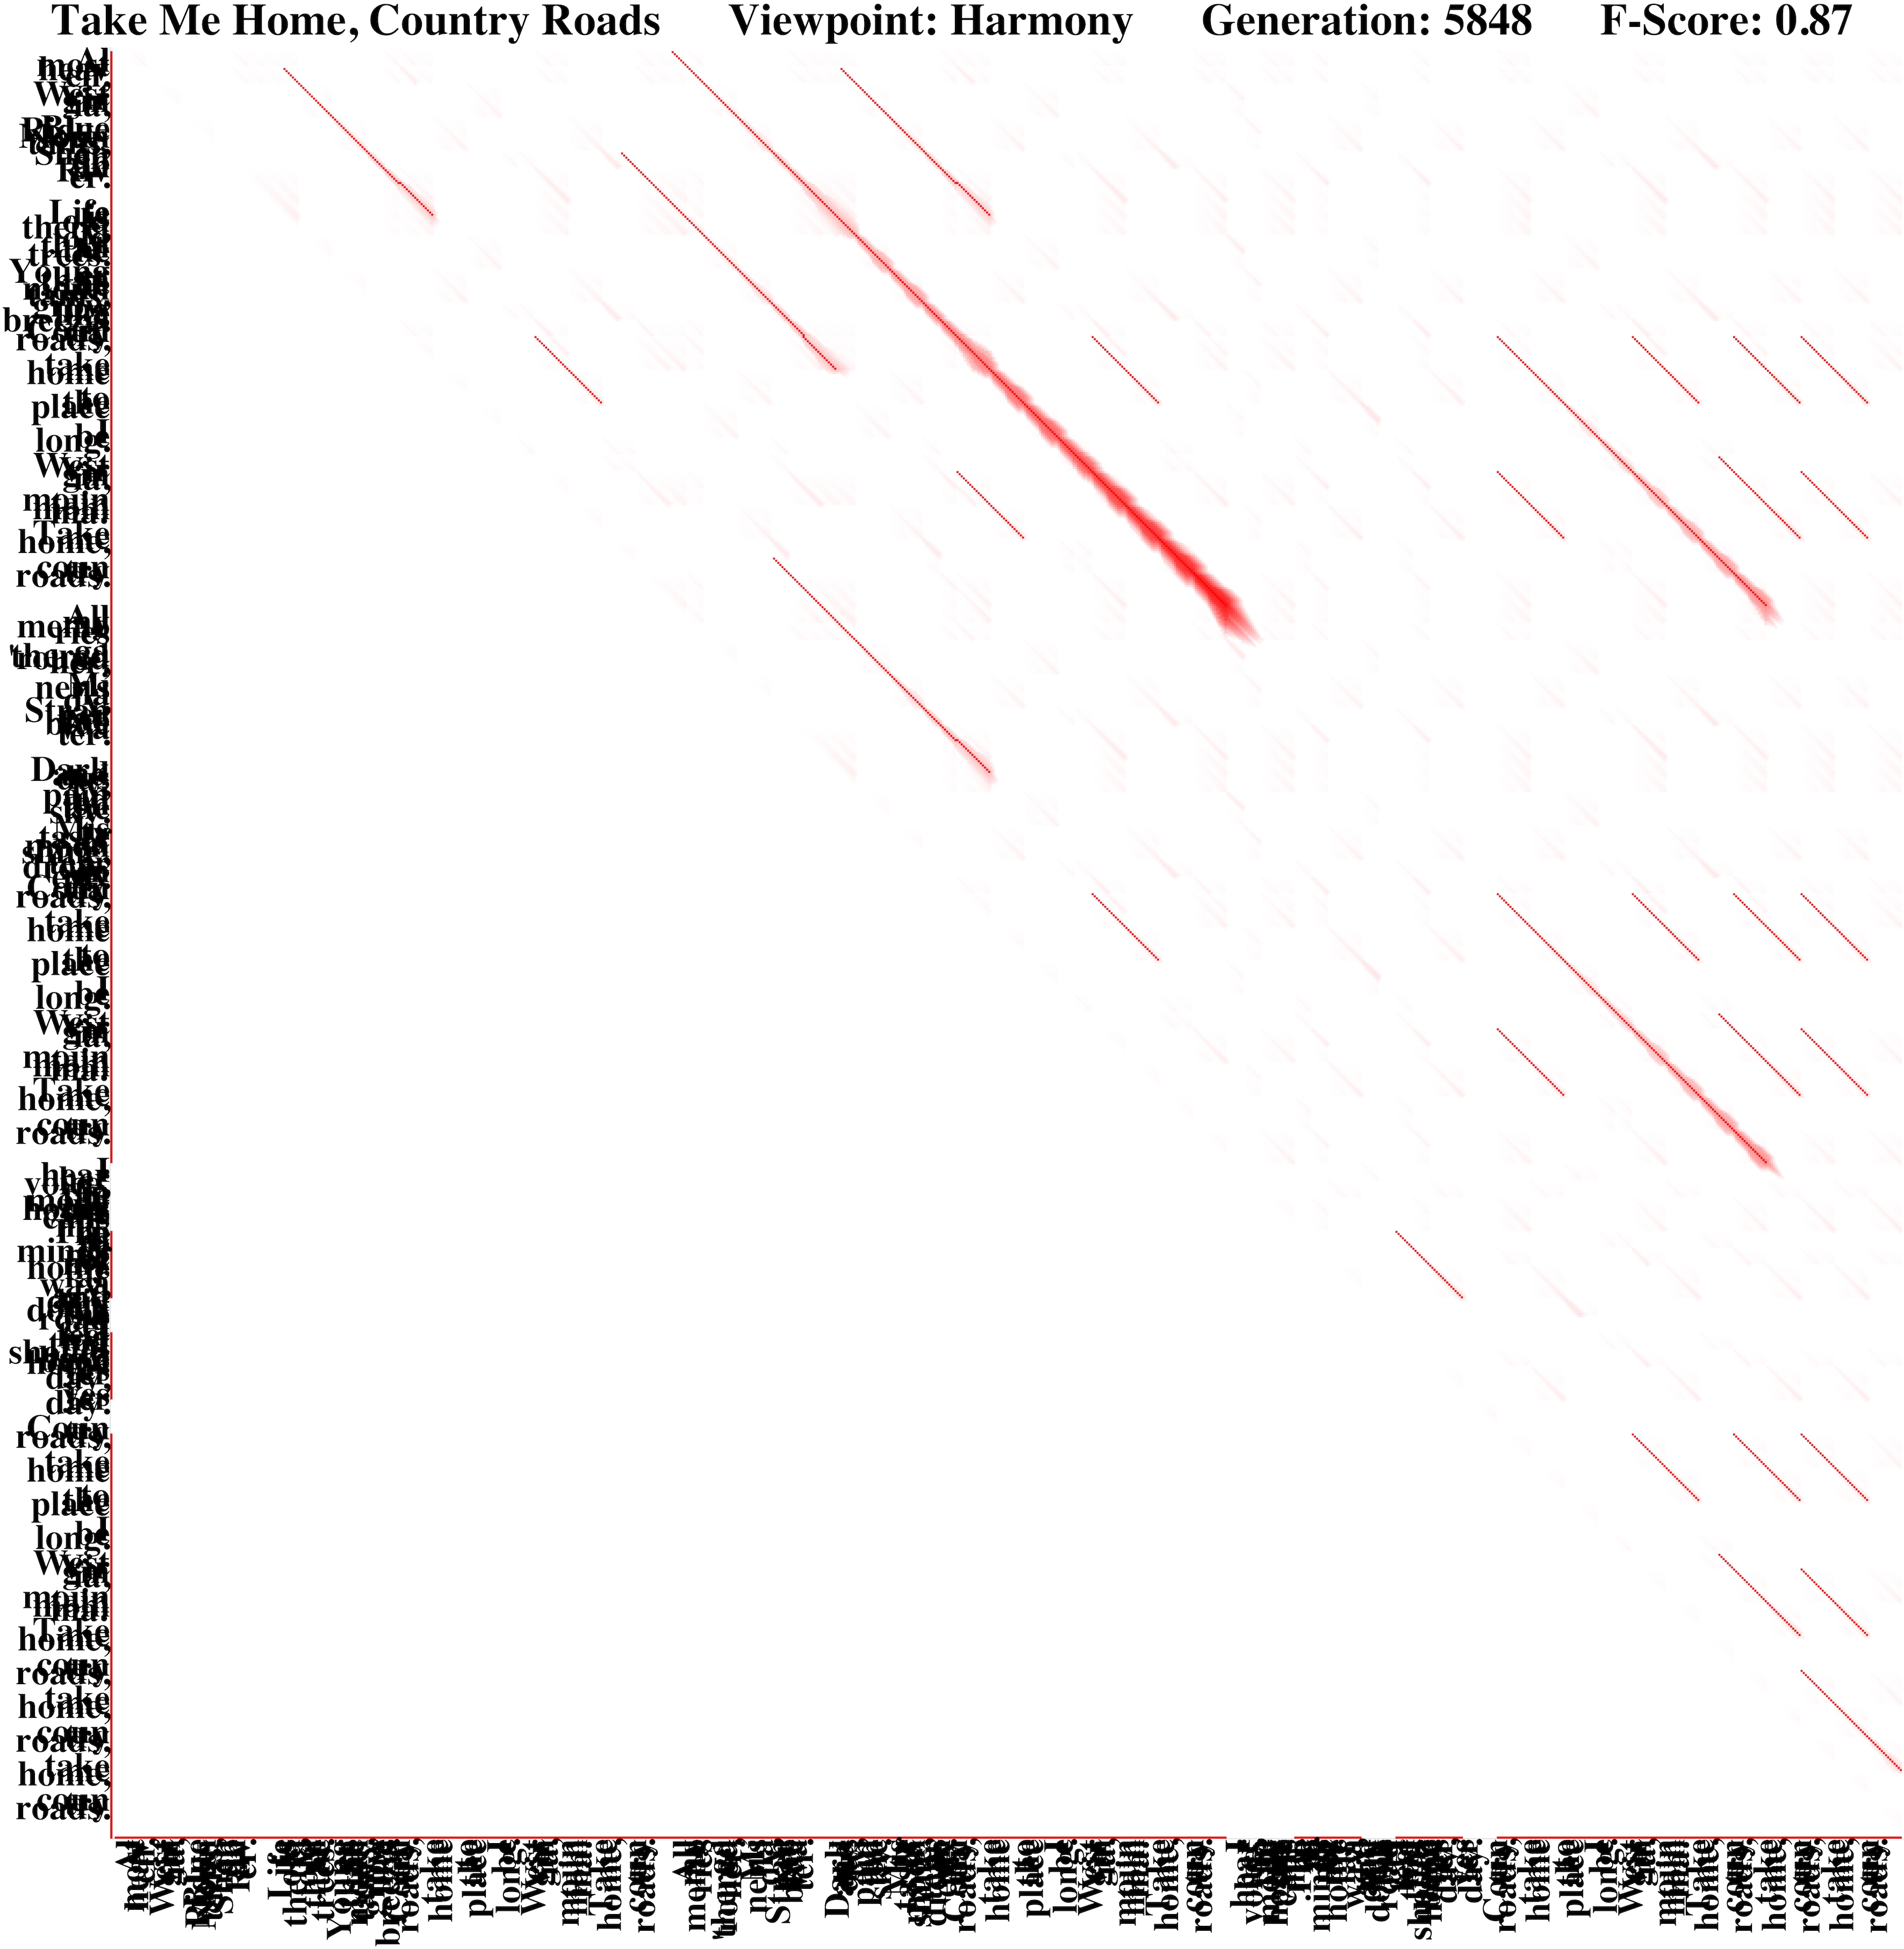
\includegraphics[width=\colwidth]{Take_Me_Home__Country_Roads_gen5848_id631_harmony} & 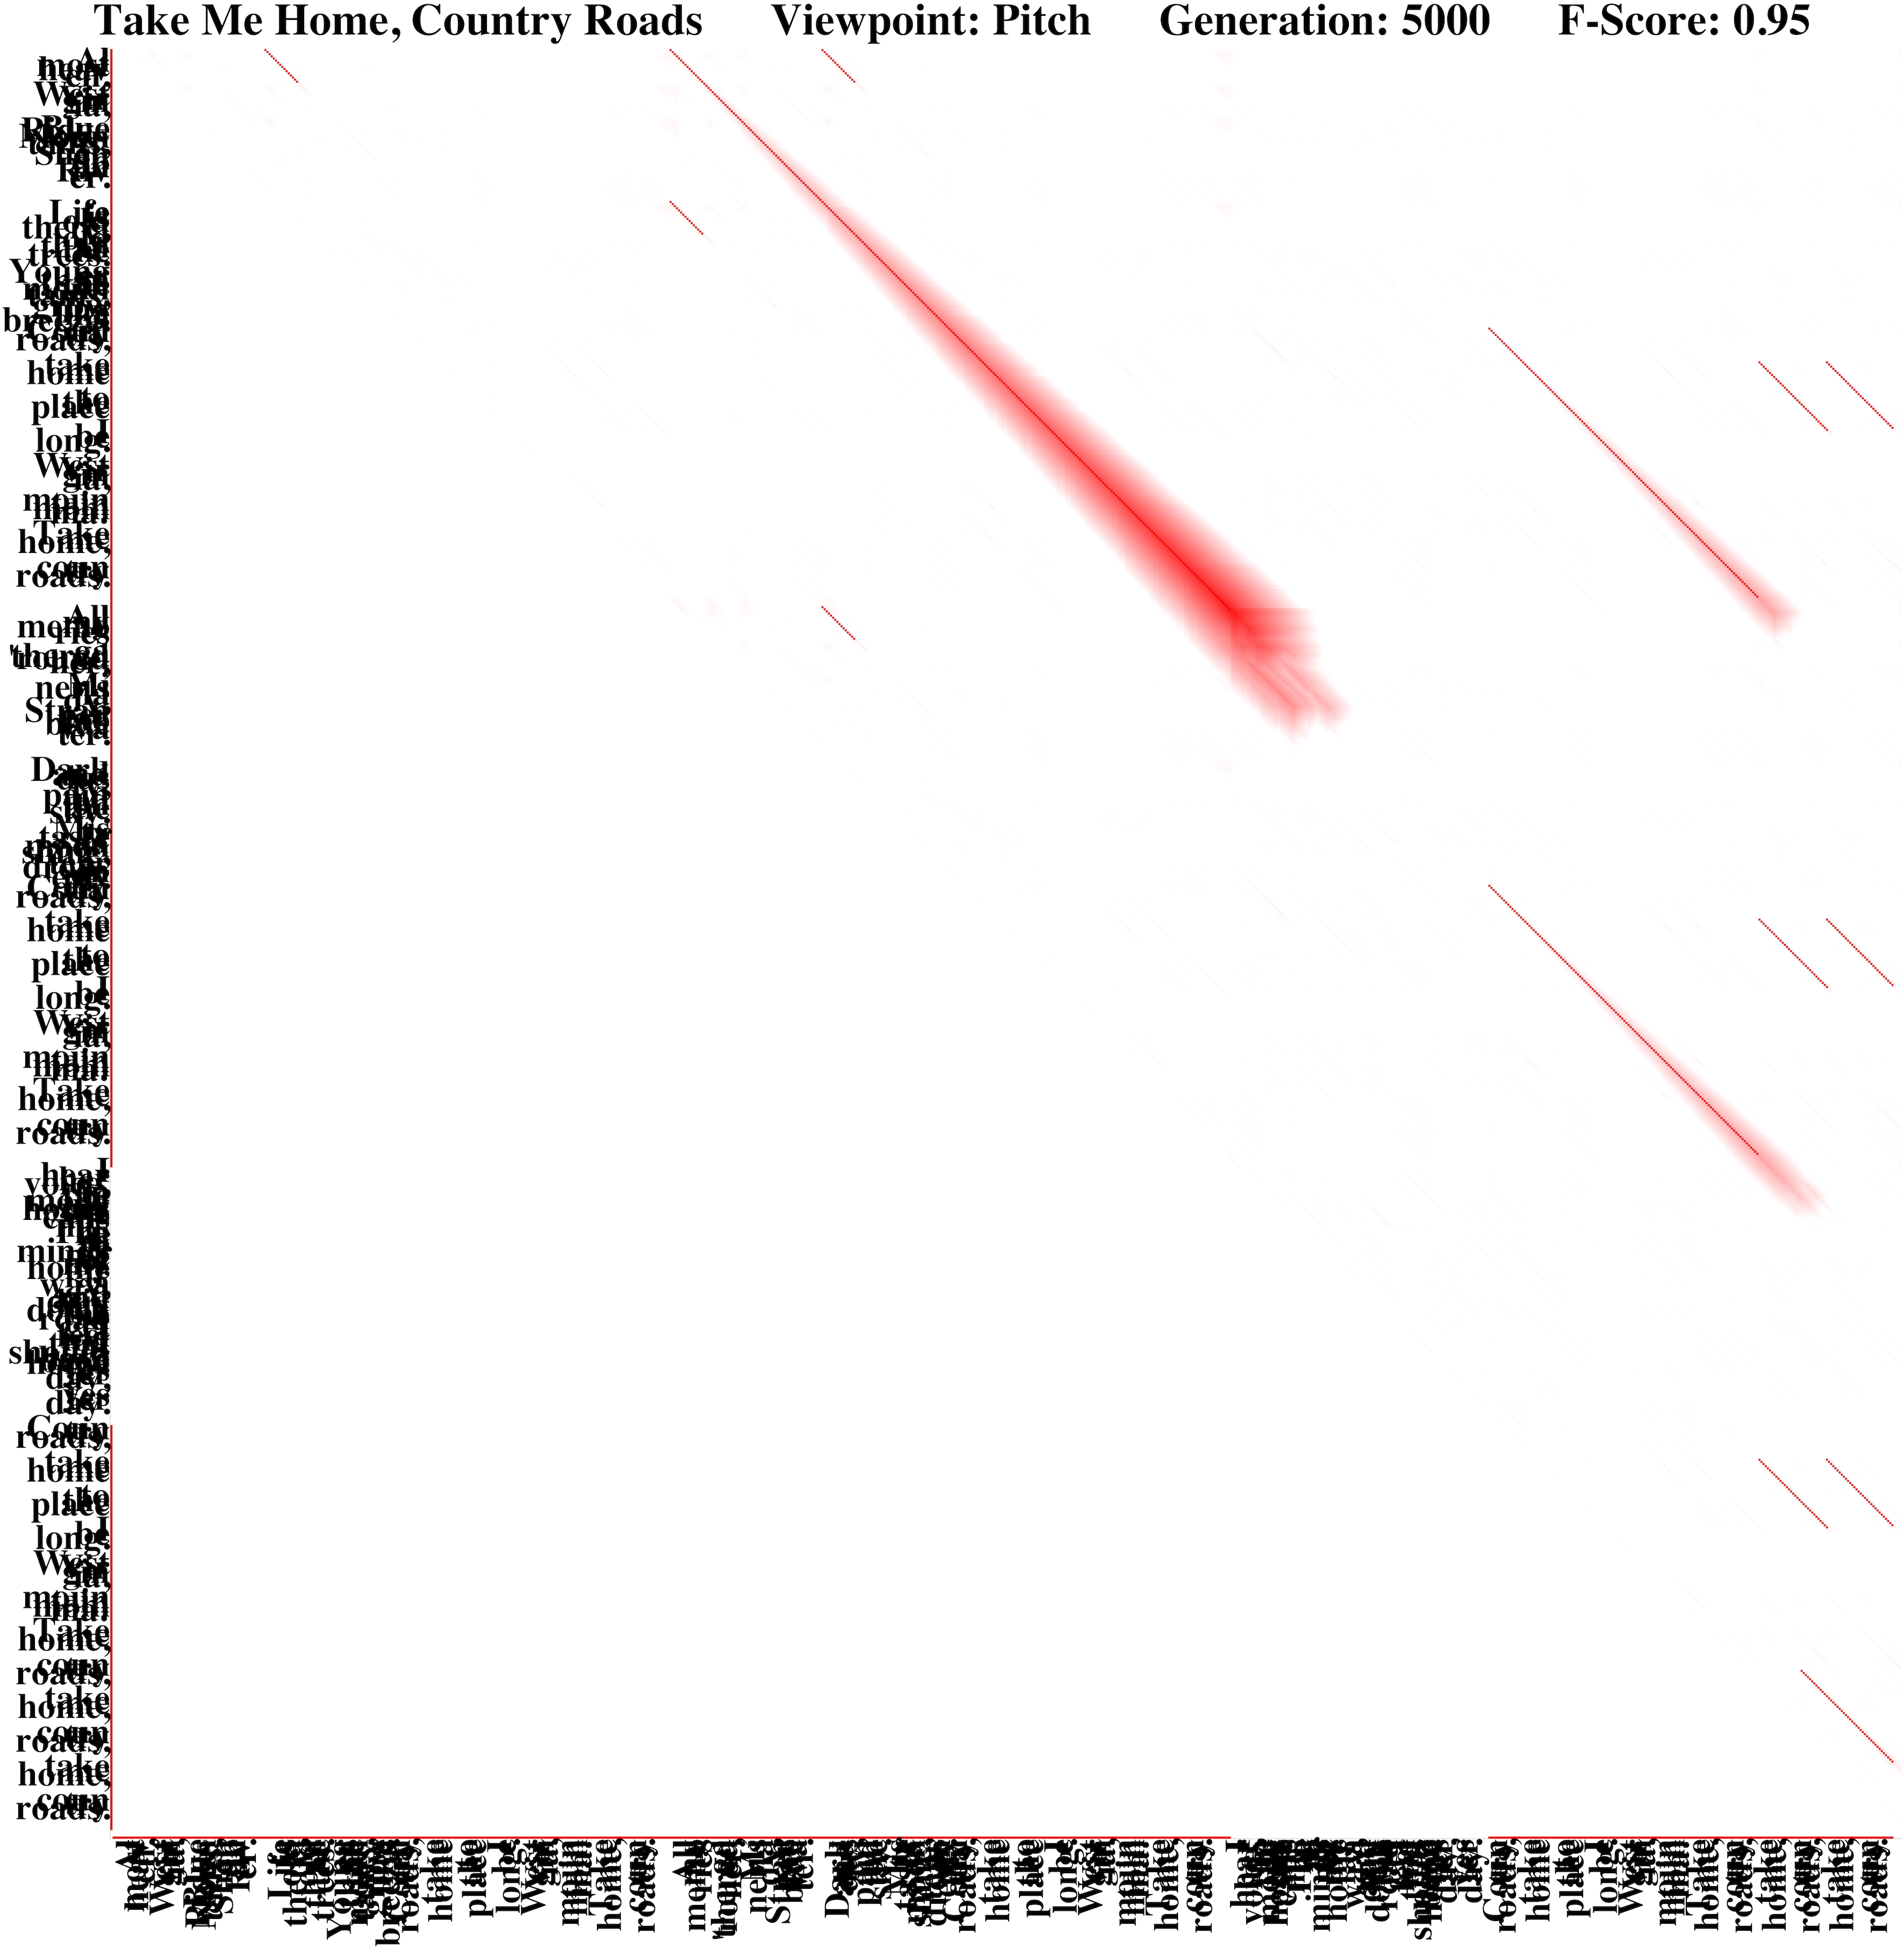
\includegraphics[width=\colwidth]{Take_Me_Home__Country_Roads_gen5000_id544_pitch} & 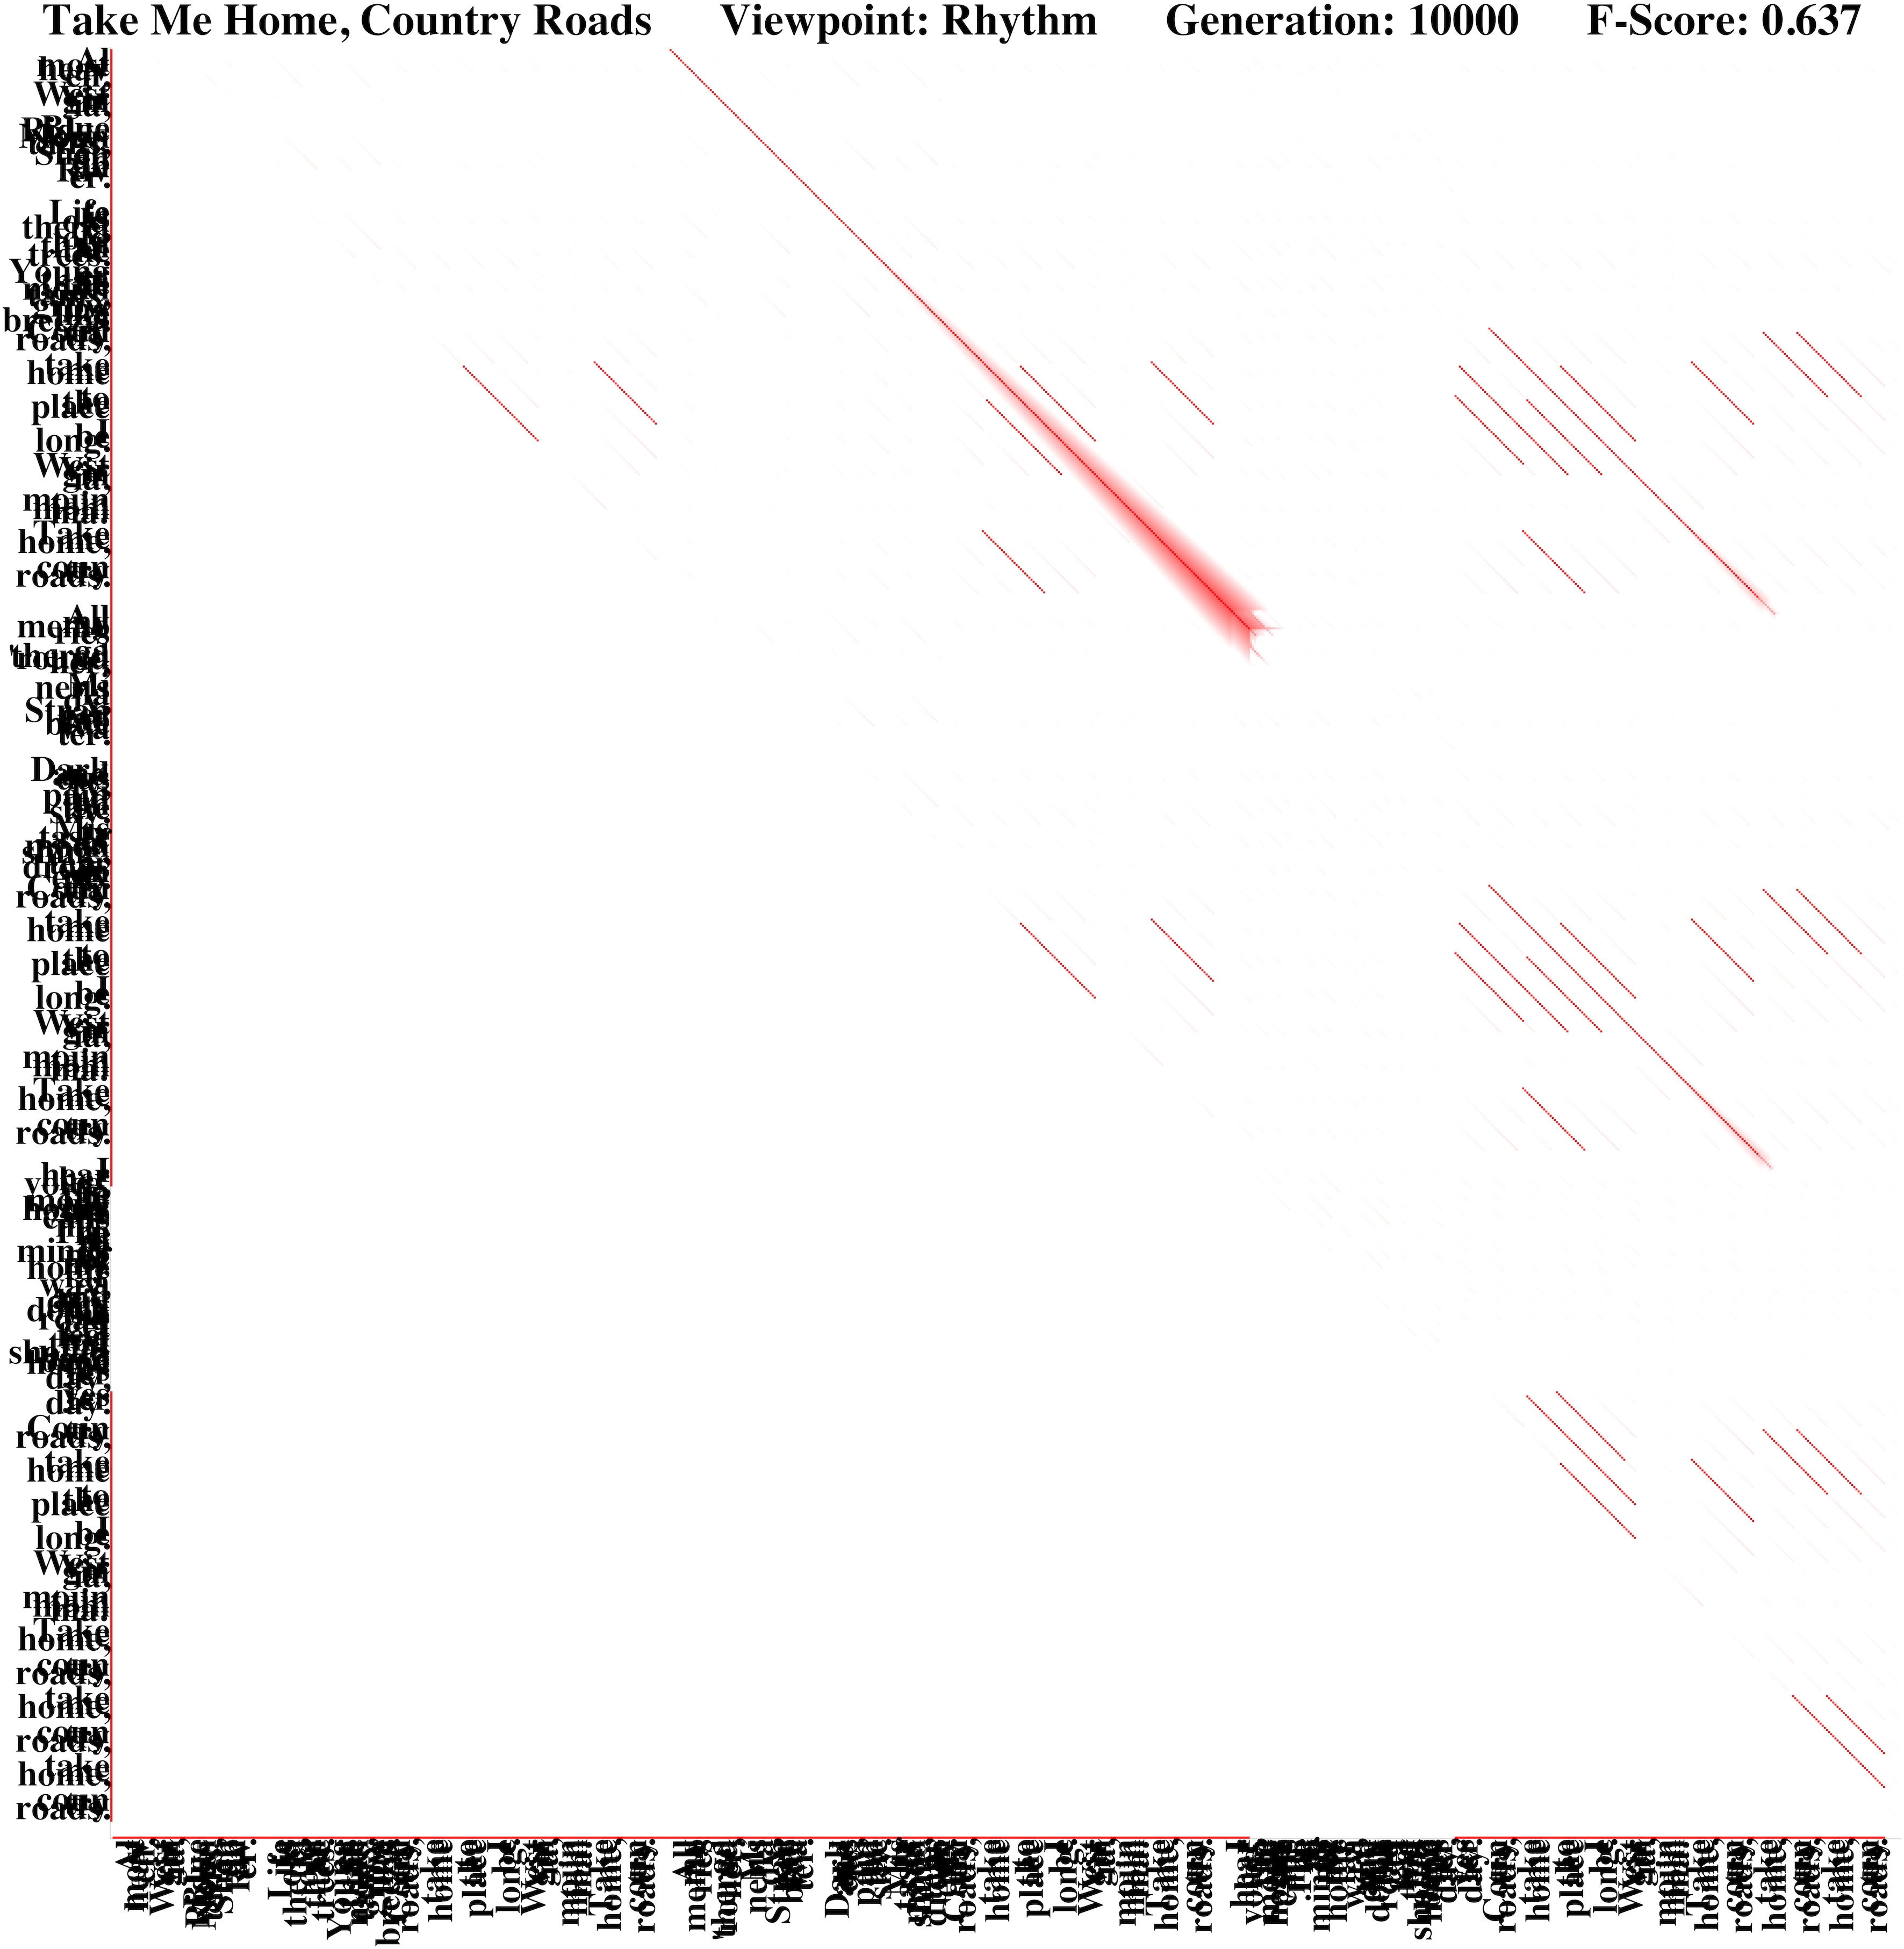
\includegraphics[width=\colwidth]{Take_Me_Home__Country_Roads_gen10000_id784_rhythm} & 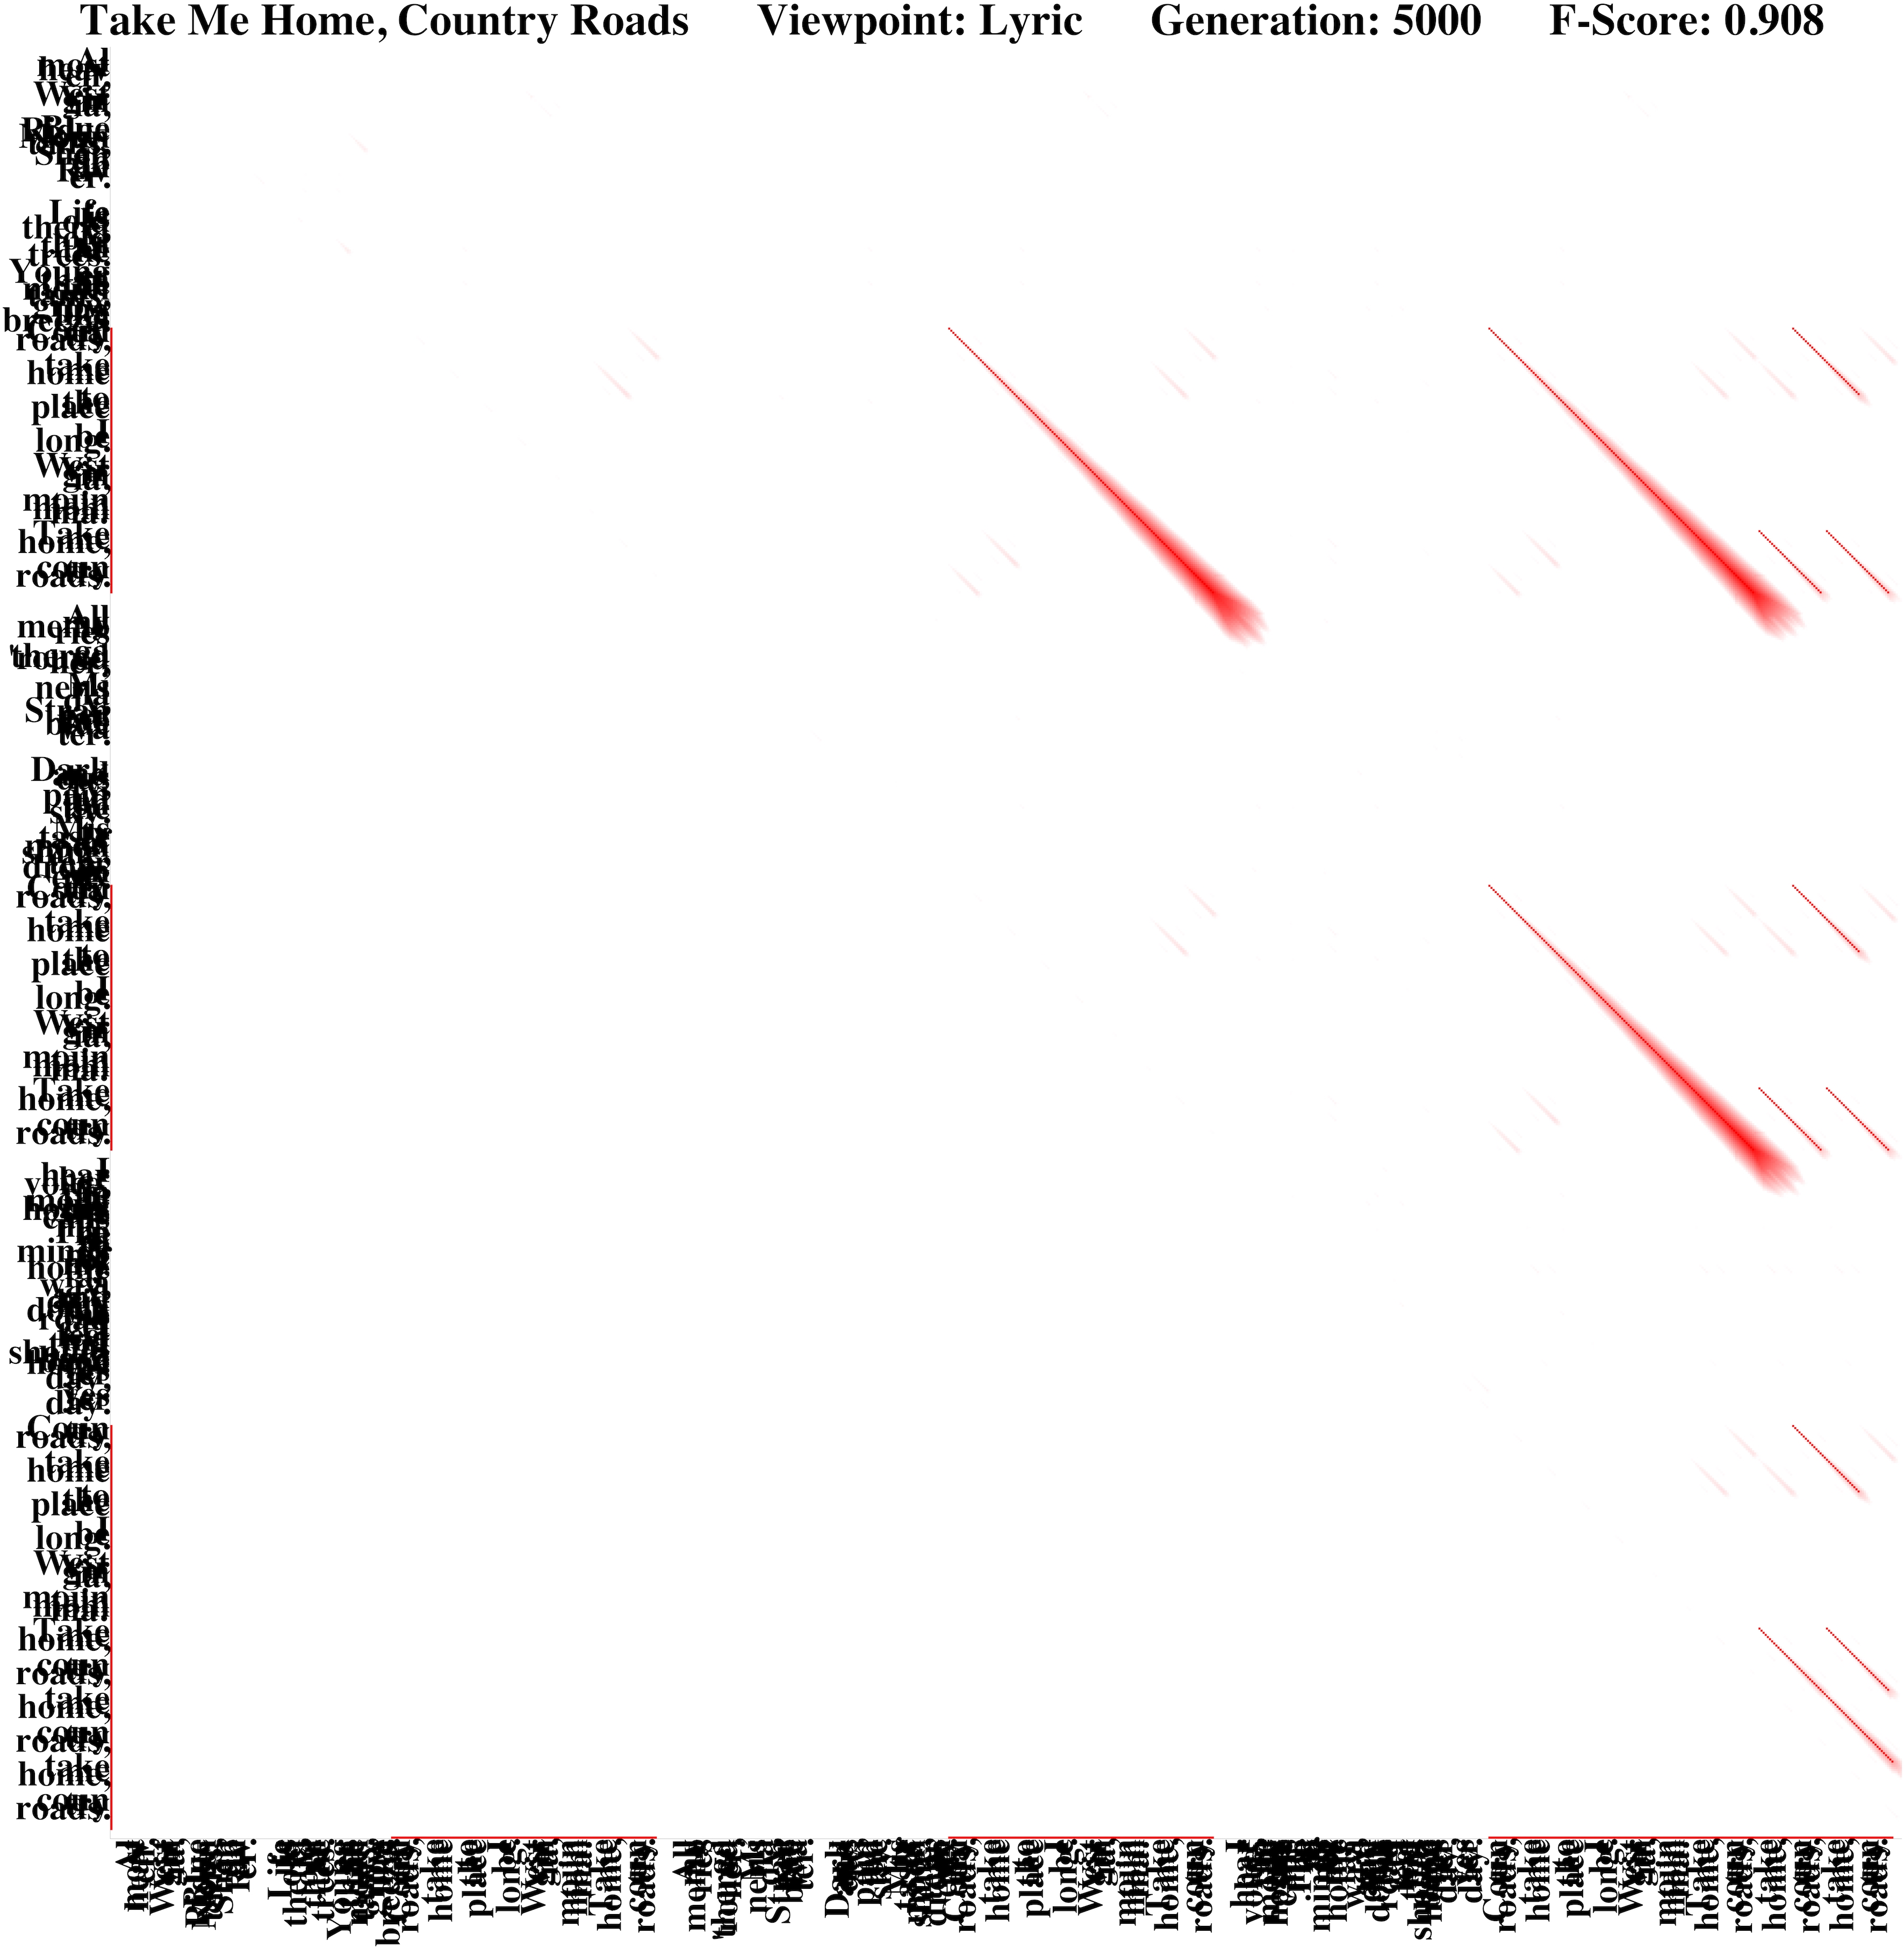
\includegraphics[width=\colwidth]{Take_Me_Home__Country_Roads_gen5000_id435_lyric} & 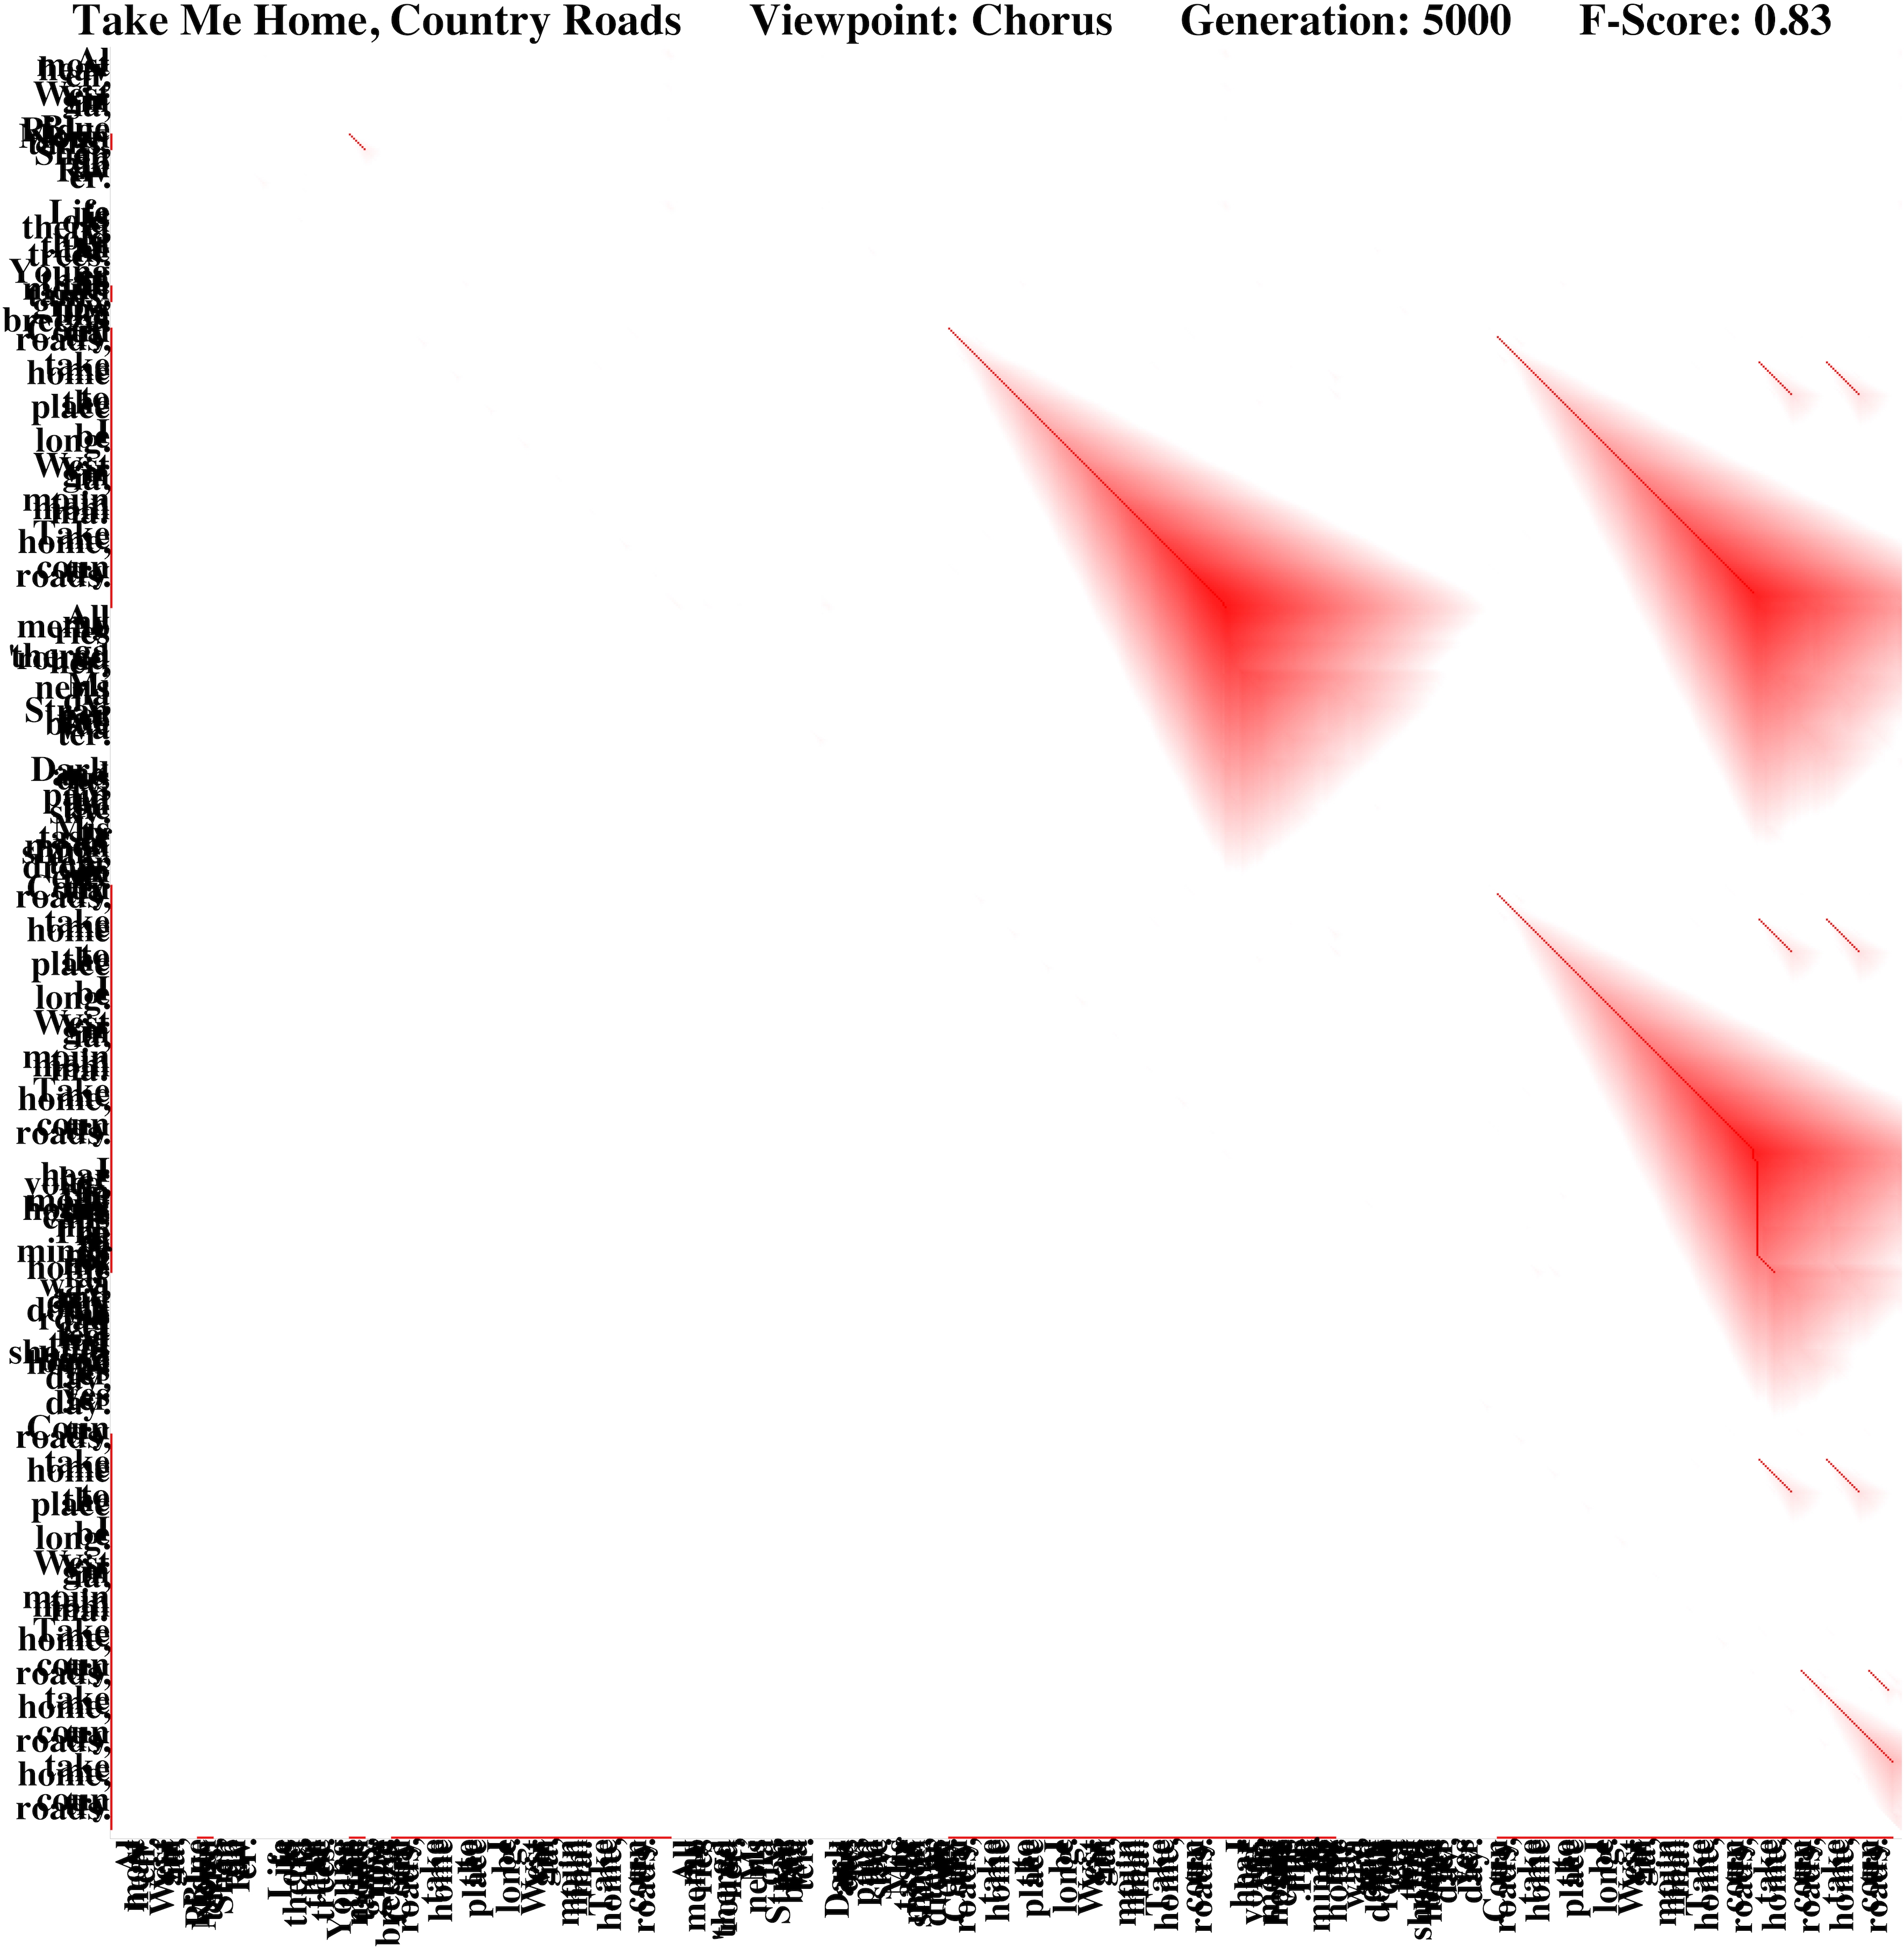
\includegraphics[width=\colwidth]{Take_Me_Home__Country_Roads_gen5000_id399_chorus} & \includegraphics[width=\colwidth]{Take_Me_Home__Country_Roads_gen5000_id467_verse} \\
% & F-Score:0.87 & F-Score:0.94 & F-Score:0.58 & F-Score:0.91 & F-Score:0.98 & F-Score:0.00 \\
\textbf{Imagine} $F_{1}=0.81$ & \includegraphics[width=\colwidth]{Imagine_gen5848_id631_harmony} & \includegraphics[width=\colwidth]{Imagine_gen5000_id544_pitch} & \includegraphics[width=\colwidth]{Imagine_gen10000_id784_rhythm} & \includegraphics[width=\colwidth]{Imagine_gen5000_id435_lyric} & \includegraphics[width=\colwidth]{Imagine_gen5000_id399_chorus} & \includegraphics[width=\colwidth]{Imagine_gen5000_id467_verse} \\
% & F-Score:0.94 & F-Score:0.87 & F-Score:0.71 & F-Score:0.93 & F-Score:0.53 & F-Score:0.00 \\
\end{tabular}
\caption{\label{fig:song_v_viewpoint}\textit{Structure Detection}. For each viewpoint (i.e., column), the same scoring function weights were used. This suggests a common scoring function can be used to find viewpoint-specific structure across different songs. The \textit{Chorus} and \textit{Verse} columns use scoring functions that are a composite of the four primitive viewpoint scoring functions. Using the GA approach for finding alignment weights for each viewpoint, we can extract the structure for each viewpoint for a given song. These structural representations can then be used for subsequent analyses including classification and generation. For each viewpoint, $v$, $F_{1}$ is $F_{1}(\Gamma^*_v)$. For each song, $F_{1}$ is the average $F_{1}(\Gamma^*_v)$ across alignments for all viewpoints $v$ for that song only.}
\end{figure*}

\section{Results and Discussion}

For each primitive viewpoint $v$ we trained for 5000 generations to find the parameterization $\Gamma^*_v$ which maximized $F_1(\Gamma_v)$ on the training data% (see Figure~\ref{fig:final_weights}) %Dan dropped
. These parameterizations then are used to identify structure in several songs (see Figure~\ref{fig:song_v_viewpoint}). We also tested for how well results generalize to an independent dataset (Table~\ref{tab:generalization}).

\begin{table}
\centering
\begin{tabular}{lllllll}
                     & H & P & R & L & C & V \\
\hline \\ [-1.5ex]
Train & 0.90    & 0.95  & 0.73   & 0.82  & .79  & .75     \\
Test     & 0.83    & 0.88  & 0.66   & 0.75  & .52      & .50  \\ 
\hline \\ [-1.5ex]
Train (hard) & 0.90    & 0.94  & 0.69   & 0.89  & 0.74   & .67   \\
Test (easy)     & 0.84    & 0.99  & 0.91   & 1.00  & 0.75   & 1.00 \\
\hline
\end{tabular}
\caption{\textit{Generalizability}. (Top) Shown are average F-scores for training and test sets resulting from a 5-fold cross-validation on a 5-song dataset (1000 generations). (Bottom) Results aggregated from 2 of the 5 cross-folds in which the holdout song is of simpler composition (\textit{Twinkle, Twinkle} and \textit{Over the Rainbow}). Results suggest that even with limited training, generalization is possible, particularly when generalizing to compositions with complexity less than or equal to that represented in the training set.}
\label{tab:generalization}
\end{table}

Each row in Figure~\ref{fig:song_v_viewpoint} effectively represents a 6-faceted structure of a song. Note that within each column, patterns across primitive viewpoints emerge, ultimately combining to yield structural information about abstract features. Notice, for example, how the overlapping across the first 4 columns effectively identifies the choruses of a song whereas overlapping the first 3 and subtracting the 4th effectively identifies the verses. These patterns reinforce the notion that each song has a characteristic abstract structure that is learnable via MSW self-alignment.

Significant patterns also emerge within columns. Harmonic and pitch structure, for example, tend to show up in longer isolated bands with limited horizontal (or vertical) overlap. Rhythmic structure often shows up as ``pyramids'' of lines with significant horizontal overlap. These patterns point to the fact that rhythmic structure is far more frequent and even \textit{hierarchical} as compared to structure in other viewpoints. Lyric structure is similar to harmony and pitch structure, but with fewer, sometimes shorter bands. This points to the fact that patterns in harmony and pitch usually span longer ranges within a song whereas lyric patterns are made up of short, dispersed repetitions.

Song-specific and viewpoint-specific structural trends are significant for different reasons. Song-specific trends make it possible to effectively compare the similarity of two songs at an abstract, musical level. This has implications for being able to classify music, recognize different arrangements of the same song, and recommend music with similar structural elements. Viewpoint-specific trends are significant in being able to generate novel structures for novel music, aiding song-writers and musical metacreationists to discover novel, meaningful structures. These trends have implications for probabilistic parsing, referring to the ability to compute a probability representing how well a musical sequence fits within a particular genre or appeals to a particular audience.

The approach, results, and implications we have demonstrated are not constrained to the symbolic music domain---similar functions, alignments, and patterns can be derived in other domains. For example, MSW self-alignment applied to musical audio signals can be used for chorus-detection, an area that has garnered significant interest (e.g., \cite{gao2015octave}). MSW self-alignment applied to linguistic features of poetry or lyrics can be used for rhyme scheme detection.

The ability to infer abstract structural features demonstrated here imbues computational systems with the ability to analyze artefacts in a way that more closely approaches their underlying meanings and intentions.

\chapter{Binary Relational Constraints in Non-Homogeneous Markov Models}

\emph{We plan to submit this paper to the 2018 Association for the Advancement of Artificial Intelligence Conference on Artificial Intelligence}

\section{Introduction}

Structure is often observed or created in sequential data as a result of relationships between elements at potentially distant positions. Protein and RNA folding depend on bonds formed by the pairing of amino acids and ribonucleotide bases respectively at various intervals. In natural language subject-verb and pronoun-antecedent agreements depend on the correct pairing of potentially distant words. Other examples of sequencing problems with relational structures might include the rostering and car sequencing problems.

In this paper we are interested in the problem of probabilistically modeling sequences under \textit{relational constraints}, that is sequences in which values at distant positions within the sequence are constrained to relate according to an arbitrary predefined relation (e.g., matching, bonding, agreement, etc.). Owing to their stochasticity, Markovian sequential data models struggle to account for structure beyond the Markov window which results in a limited ability to generate or classify sequences in problem domains characterized by such structures. 

Much work has been done to impose structure in Markov processes by combining such processes with constraint programming (CP) and constrained probabilistic modeling techniques. Non-homogeneous Markov models (NHMMs) \cite{pachet2011finite} generate finite-length sequences which adhere to a set of unary constraints with probabilities determined from a Markov process.

Recent work has focused on statistical models which obey \textit{regular constraints}. A regular constraint on a sequence of finite-domain variables is a constraint that requires that the corresponding sequence of values taken by these variables belongs to a given regular language \cite{pesant2004regular}. These models are convenient because they can effect structure without imposing unary constraints at fixed positions. \cite{papadopoulos2014avoiding} demonstrate how a regular constraint in the form of a deterministic finite automaton (DFA) can be combined with probabilistic Markov model to create a model that generates sequences belonging to the language of the automaton with probability approximately equal to the Markov probability distribution. Their follow-up work devises a belief propagation model in the form of a factor graph capable of exact sampling of sequences under arbitrary regular and Markov constraints \cite{papadopoulos2015exact}.

Relational constraints can often not be characterized using regular languages (e.g.,  $A = \{ww\mid w\in{a,b}*\}$ or $A = \{ww\mid w\in\Sigma\}$ where $\Sigma$ is an infinite domain). However, under the assumptions of finite-domain variables and finite-length sequences, relational constraints can be modeled using regular constraints. This suggests that an approach similar to that of \cite{papadopoulos2015exact} may be suitable for imposing relational constraints given a method for proper DFA construction.

In what follows we detail the formulation of a regular constraint (in the form of a DFA) from an arbitrary set of relational constraints. We also detail a method for exact probabilistic sampling of sequences from the language an arbitrary DFA which uses NHMMs and demonstrate its improved efficiency over factor graphs for sampling large batches of constrained sequences. 

\section{Related Work}

Several works have been presented which address the problem of imposing relational constraints.

\cite{barbieri2012markov} demonstrate examples of how unary constraints can be used to imitate relational rhyming constraints. This approach is not suitable for most relational constraint applications as it relies on separately constraining values at independent positions rather than constraining based on the comparison of values. 

\cite{bodily2018floating} demonstrate that arbitrary relational constraints can be effected in $d$-order NHMMs but only when matching positions are within the Markov window (i.e., at most $d$ sequence positions apart). The method we present has no limitation on the distance between relationally constrained positions.

\cite{roy2016enforcing} define an Allen constraint as a global constraint relating indices with temporal positions. This work is designed to primarily address contiguous temporal sequences in which temporal positions and sequence indices are not directly related. Their interest is primarily in sub-sequence \textit{equality} constraints. The algorithm for how these constraints are effectuated is not presented.

\cite{collins2017computer} create long-term repetitive and phrasal structure in music using a ``copy-paste'' approach to enforce binary matching of full sequences at intervals. This approach is fundamentally non-Markovian at splice sites causing unnatural transitions at splice sites. \cite{pachet2017sampling} present a similar ``copy-paste'' method for creating structured music lead sheets, but use a controlled variation mechanism to ensure that copies are contextually situated to satisfy Markovian properties.

To our knowledge, the method described below is novel in its strict use of Markovian processes (of arbitrary order) for generation while simultaneously enforcing arbitrary relational constraints at arbitrary distances.

\section{A DFA for Relational Constraints}

A \textit{binary relation} $\rho$ on a set $\Sigma$ is defined as a set of ordered pairs of elements of $\Sigma$. Examples include the set of pairs of amino acids $(x,y)$ such that $x$ forms a bond with $y$; or the set of ordered pairs of words $(x,y)$ such that $x$ is an antecedent and $y$ is a pronoun that agrees with $x$.

In generating a sequence of random variables $X=(X_1,\mydots,X_n)$ we define a \textit{relational constraint} $(X_i,X_j,\rho)$ for an arbitrary binary relation $\rho$ to mean that the values $x_i$ and $x_j$ assigned to the variables $X_i$ and $X_j$ are constrained so as to ensure that $(x_i,x_j)\in\rho$. A partially instantiated relational constraint of the form $(x_i,X_j,\rho)$ or $(X_i,x_j,\rho)$ represents a unary constraint in which $X_i$ or $X_j$ has been further constrained to the values $x_i$ or $x_j$ respectively.

A DFA, or simply an automaton, is defined as a quintuple $\mathcal{A} = \langle Q, \Sigma, \delta, q_0, F\rangle$ in which:
\begin{itemize}
\item $Q$ is a finite set of states;
\item $\Sigma$ is a finite set of symbols termed the alphabet;
\item $q_0 \in Q$ is the initial or start state of the automaton;
\item $\delta$ is the transition function $Q \times \Sigma \rightarrow Q$, mapping a state to a successor state for a given symbol;
\item $F \subseteq Q$ is the set of final or accept states.
\end{itemize}

A sequence $s = \{s_1,\mydots,s_n\}$ is \textit{accepted} by $\mathcal{A}$ iff there exists a sequence $q_0,\mydots, q_n$ of states such that $\forall i, 1 \leq i \leq n$, $\delta(q_{i-1},s_i) = q_i$ and $q_n\in F$. The language $\mathcal{L}(\mathcal{A})$ is the set of all sequences which $\mathcal{A}$ accepts.

A Markov model is a stochastic process where the probability of a sequence of random variables $X=(X_1,\mydots,X_n)$ is computed as $P(X)=P(X_1)\cdot P(X_2\mid X_1)\cdots P(X_n\mid X_{n-1})$. As such a Markov model consists of a set of initial probabilities $\mathcal{I}$ for each state and a set of transition probabilities $\mathcal{T}$ between states. Note that when combining a DFA and Markov model, the domain $\Sigma$ for variables $X_1,\mydots,X_n$ is the same as the alphabet $\Sigma$ for the DFA.
\newcommand{\gbfs}{\ensuremath{\mbox{\sc Relational Automaton}}}
\renewcommand{\algorithmicrequire}{\textbf{Data:}}
\renewcommand{\algorithmicensure}{\textbf{Result:}}
\begin{algorithm}[!b]
\caption{$\gbfs$}\label{alg:matching} 
\begin{algorithmic}
%\medskip
\Require{$n$ a sequence length}\newline
$\mathcal{M}$ a set of binary relational constraints \newline
$I$ a set of valid initial states \newline
$T$ a set of valid transitions
\Ensure{$\mathcal{A}$ a DFA for $\mathcal{M}$}
\State{$\mathcal{A} \leftarrow \langle Q, \Sigma, \delta, q_0, F \rangle$}
\State{$S \leftarrow \{\langle\emptyset,I,q_0\rangle\}$} 

\For{$i \leftarrow 1$ to $n-1$}
  \State{$S'\leftarrow\{\}$}
  \For{$\langle C,V,q\rangle \in S$}
    \For{$v \in V$}
      \State{$C'\leftarrow \{(A,B,\rho)\in C\mid A\neq X_i \land B\neq X_i\}$}
      \For{$(X_j,X_k,\rho)\in\mathcal{M}$}
      	\If{$i=j$ and $j<k$}
      		\State{$C' \leftarrow C' \cup (v,X_k,\rho)$} %\Comment{add new constraint}
      	\EndIf
        \If{$i=k$ and $k<j$}
      		\State{$C' \leftarrow C' \cup (X_j,v,\rho)$} %\Comment{add new constraint}
      	\EndIf
      \EndFor
      \State{$V' \leftarrow \emptyset$} \Comment{initialize possible next states}
      \For{$vv_2\in T$} \Comment{filter by $C'$}
      	\If{$\forall (v',X_{i+1},\rho)$$\in$$C', (v',v_2)\in\rho$}
      		\If{$\forall (X_{i+1},v',\rho)$$\in$$C', (v_2,v')\in\rho$}
				\State{$V' \leftarrow V' \cup v_2$}
        	\EndIf
		\EndIf
      \EndFor
      \If{$V' \neq \emptyset$} \Comment{if not a dead state}
      	\If{$\exists q_i$ s.t. $\langle C',V',q_i\rangle \in S'$}
        	\State{$q' \leftarrow q_i$}
        \Else
        	\State{$q' \leftarrow NewState(Q)$}
            \State{$S'\leftarrow S' \cup \langle C',V',q'\rangle$}
        \EndIf
        \State{$\delta(q,v) \leftarrow q'$} \Comment{extend path}
%         \If{$\exists L$ s.t. $\langle q',q,L\rangle \in b$}
%         	\State{$L \leftarrow L \cup v$}
%         \Else
%         	\State{$b \leftarrow b \cup \langle q',q,\{v\}\rangle$}
%         \EndIf{}
      \EndIf
    \EndFor
%     \If{$\nexists v$ s.t. $\delta(q,v)$ is defined} \Comment{nothing added}
%     	\If{$removeState(q) = false$}
%         	\State{\Return{$null$} \Comment{unsatisfiable}}
%         \EndIf
%     \EndIf
  \EndFor
  \If{$S' = \emptyset$}
  	\State{\Return{$null$}} \Comment{unsatisfiable}
  \EndIf
  \State{$S \leftarrow S'$}
\EndFor
\State{$q_{acc} \leftarrow NewState(Q)$} \Comment{define accepting state}
\State{$F \leftarrow F \cup q_{acc}$}
\For{$\langle C,V,q\rangle \in S$}
  \For{$v \in V$}
  	\State{$\delta(q,v) \leftarrow q_{acc}$}	
  \EndFor
\EndFor
\State{\Return{$\mathcal{A}$}}

% \Statex
% \Function{$removeState$}{$q$}
% 	\State{$R \leftarrow \{q\}$}
%     \While{$R \neq \emptyset$}
%     	\State{$q_r \leftarrow poll(R)$}
%         \If{$q_r = q_0$}
%         	\State{\Return{$false$}} \Comment{unsatisfiable}
%         \EndIf
%         \For{$q',L$ s.t. $\langle q_r,q',L\rangle \in b$}
%         	\State{$b \leftarrow b / \langle q_r,q',L\rangle$}
%         	\For{$l \in L$}
%             	\State{$\delta \leftarrow \delta /\delta(q',l)$}
%             \EndFor
%     		\If{$\nexists v$ s.t. $\delta(q',v)$ is defined}
%             	\State{$R \leftarrow R \cup q'$} \Comment{remove new dead state}
%             \EndIf
%         \EndFor
%         \State
%     \EndWhile
%     \State{\Return{$true$}}
% \EndFunction
\end{algorithmic}
\end{algorithm}

Given a set of binary relational constraints $\mathcal{M} = \{(X_i,X_j,\rho)\}$, a set of valid start symbols $I\subset\Sigma$, a set of valid transitions $T=\{s_is_j\mid s_i\in\Sigma$ and $s_j\in\Sigma\}$, and a length $n$, Algorithm~\ref{alg:matching} creates a DFA $\mathcal{A}$ such that $\mathcal{L}(\mathcal{A})$ is the set of all sequences  $s\in\Sigma^n$ such that $s_1\in I$; $s_{i-1}s_i\in T$ for all $i, 1 < i \leq n$; and $(s_j,s_k)\in\rho$ for all relational constraints $(X_j,X_k,\rho)$ in $\mathcal{M}$. Where $I$ and $T$ are derived from the sets $\mathcal{I}$ and $\mathcal{T}$ of a Markov model $M$, this means $p_M(s) > 0$.

\begin{figure*}
    \centering
    \includegraphics[width=.8\textwidth]{DFA}
    \caption{\textit{A {\sc Relational} automaton}. The result of Algorithm~\ref{alg:matching} on inputs $n=4$; $\mathcal{M}=\{(X_1,X_4,\rho\}$ (where $\rho$ represents the set of rhyming word pairs); $I=\{$\textit{Mary}, \textit{Clay}$\}$; and $T$ derived from the non-zero transitions represented in the Markov model shown in Figure~\ref{fig:markov}.}
    \label{fig:DFA}
\end{figure*}

The algorithm takes the general approach of building breadthwise a tree-like DFA where each layer (of edges) in the tree represents a position in the sequence to be generated. Each state $q_i$ is defined by a triple $<C,V,q_i>$ where $C = \{(X_i,X_j,\rho)\}$ is the set of relational constraints that are guaranteed from the state; $V=\{x\mid x\in\Sigma\}$ is the set of valid labels \emph{allowed} by $T$ for edges originating from the state (in practice dead states and paths may be pruned); and $q_i$ is a reference to the state itself.

When expanding the path via a state $q_i$ associated with sequence position $i$ and triple $<C,V,q_i>$, a new path is considered for every label $v\in V$. In order to build the path, the algorithm first computes what would be the new triple $<C',V',q'>$ for the new state reached via $v$ in order to check if such a state already exists. The new set $C'$ inherits all constraints from $C$ except those already satisfied at sequence position $i$ and adds new constraints applying to position $i$ in their partially instantiated form using $v$. The new set $V'$ is populated with the set of all labels $v_2$ that are 1) valid transitions from $v$ according to $T$ and 2) satisfying values for any constraints in $C'$ which apply to sequence position $i+1$. In practice, $V'$ can be further constrained by unary constraints or negated relational constraints (i.e., constraining to ensure $(x_i,x_j)\not\in\rho$) to further prune undesirable sequences. Assuming $V'$ is not empty (a sign of a dead state), we check for an existing state associated with sequence position $i+1$ and triple $<C',V',q'>$ or create a new one which is then used to extend the path. In the last state layer there is a single accepting state to which all states in the previous state layer connect via all valid labels in their respective $V$ sets. 

Figure~\ref{fig:DFA} shows the DFA built using Algorithm~\ref{alg:matching} with $n=4$; $\mathcal{M}=\{(X_1,X_4,\rho_{rhyme}\}$ (where $\rho_{rhyme}$ represents the set of rhyming word pairs); $I=\{$\textit{Mary}, \textit{Clay}$\}$; and $T$ derived from the non-zero transitions represented in the Markov model shown in Figure~\ref{fig:markov}.

\begin{figure}
\centering
\includegraphics[width=\linewidth]{markov}
\caption{\textit{A Markov model.}}
\label{fig:markov}
\end{figure}

The time and space requirements for the algorithm vary significantly depending on the inputs. Each constraint in $\mathcal{M}$ at a new position splits the path into a number of paths dependent on the number and distribution of transitions in $T$ and the restrictiveness of the constraint's relation $\rho$. Divergent paths will reconverge once all overlapping constraints have been resolved. The number of paths and states can also be reduced by the addition of unary constraints, negated relational constraints, increasing the number of symbols per label (i.e., increase the Markov order), and reducing the size of the transition set $T$.

One way to optimize the construction of a {\sc Relational} automaton is to take advantage of binary relational constraints for which $\rho$ is an \emph{equivalence relation} (i.e., reflexive, symmetric, and transitive). In such cases many partially instantiated constraints become equivalent. For example, under the equivalence relation of rhyming (allowing for a word to rhyme with itself), the following partially instantiated binary relational constraints are equivalent: $(Mary,X_4,\rho),(Fairy,X_4,\rho),(Carry,X_4,\rho)$. These constraints can all be represented using a generalized constraint that uses the equivalence class $\mathcal{E}_{Mary}$ representing the set of all rhyming word pairs that rhyme with ``Mary'': $(\mathcal{E}_{Mary},X_4,\rho)$. This facilitates the combining of states in the DFA.

\section{Exact Sampling of Constrained Sequences}

Given a {\sc Relational} automaton $\mathcal{A}$, a Markov model $M$, a set of unary constraints $C$, and a length $n$ we now turn attention to sampling sequences from the target distribution $p^*$ defined as:

\[
  p^*(X_1,\mydots,X_n) \propto   
  \begin{cases}
	p_M(X_1,\mydots,X_n)\cdot & \text{if } X_1,\mydots,X_n \in 	\mathcal{L}(\mathcal{A})\\
    \quad \prod_{i=1}^n p_C(X_i)\\
	0 & \text{otherwise}
  \end{cases}
\]

\cite{papadopoulos2015exact} demonstrate one mechanism for computing $p^*$ that uses factor graphs with belief propagation for sampling sequences with exact probabilities according to the original distribution. In this latter solution a backward phase computes the impact on each sequential position $i$ in the factor graph of the sub-factor graph representing all positions ``to the right'' of $i$. A forward phase computes the marginal distribution over values for each sequence position $i$ given the partial instantiation for variables representing positions ``to the left'' of $i$ and simultaneously samples a sequence. A potential drawback to this solution is that though the backward phase is completed once, the forward phase is repeated each time a sequence is sampled. 

We present a novel algorithm (Algorithm~\ref{alg:nhmm}) for sampling sequences under regular and Markov constraints with exact probability that uses a NHMM \cite{pachet2011finite}. A NHMM $\mathcal{N}$ is a constrained probabilistic model constructed from a Markov model $M$, a set of unary constraints $C$, and a length $n$ such that 
\[
  p_\mathcal{N}(X_1,\mydots,X_n) \propto   
	p_M(X_1,\mydots,X_n)\cdot\prod_{i=1}^n p_C(X_i)\\
\]
Constructing a NHMM computes all marginal distributions ahead of time. This speeds up sampling time at the cost of an increased build time, making it a better choice for sampling large sets of sequences or online applications (see Figures~\ref{fig:sampleTimeByCount} and~\ref{fig:sampleTimeByLength}). A detailed explanation of NHMMs and the method of their construction (referenced as ``constructNHMM()'' in Algorithm~\ref{alg:nhmm}) is available from \cite{pachet2011finite}.

Given an automaton $\mathcal{A}=\langle Q, \Sigma, \delta, q_0, F \rangle$, a Markov model $M=\{\mathcal{I},\mathcal{T}\}$, a set of unary constraints $C=\{c_{X_i}\}$ (where $c_{X_i}$ represents a unary constraint $c$ applied to the random sequence variable $X_i$), and a length $n$, Algorithm~\ref{alg:nhmm} builds a new ``state-sensitive'' Markov model $M'$ which incorporates the regular constraint represented by $\mathcal{A}$. Each Markov label in $M'$ represents a label-state pair $<x,q>$ where $x\in\Sigma$ is a label of the original Markov model $M$ and $q\in Q$ is a state of the automaton $\mathcal{A}$. Whereas with $M$ we can directly sample values $x_1,\mydots,x_n$ for a sequence of random variables $X=X_1,\mydots,X_n$, in the ``state-sensitive'' model $M'$ we first sample values $x_1',\mydots,x_n'$  for a sequence of random label-state variables $X'=X_1',\mydots,X_n'$. We obtain $X$ through the assignment $X=x_1'.label,\mydots,x_n'.label$ where $x_i'.label$ is the value of the label in the label-state pair $x_i'$.

The set of initial probabilities $\mathcal{I}'$ of $M'$ is defined as
\[
  \mathcal{I}'(<x,q>) \propto
  \begin{cases}
	\mathcal{I}(x) & \text{if } q = \delta(q_0,x)\\
	0 & \text{otherwise}
  \end{cases}
\]
\noindent and the transition probability function $\mathcal{T}'$ of $M'$ is defined as
\[
  \mathcal{T}'(<x',q'>\mid <x,q>) \propto   
  \begin{cases}
	\mathcal{T}(x'\mid x) & \text{if } q'=\delta(q,x')\\
	0 & \text{otherwise}
  \end{cases}
\]
A new set of unary ``state-sensitive'' constraints $C'$ is also created such that for each unary constraint $c_{X_i} \in C$, an equivalent constraint $c_{X_i'.label}$ (meaning the same general constraint $c$ applied to the \textit{label} attribute of the random label-state variable $X_i'$) is added to $C'$ which applies only to the label $x$ in the new label-state pair $x'=(x,q)$. An {\sc accepting} constraint $c_{X_n'.state\in F}$ applying to $X_n'$ is also added to $C'$ to ensure that all valid Markov sequences from $M'$ end with a label-state pair $x'=(x,q)$ where $q\in F$.

The final step of Algorithm~\ref{alg:nhmm} constructs a NHMM from the unnormalized $M'$, $C'$, and $n$ using the construction set forth by \cite{pachet2011finite} which normalizes probabilities to create the target distribution $p^*$.

\newcommand{\gbfsa}{\ensuremath{\mbox{\sc Regular NHMM}}}
\renewcommand{\algorithmicrequire}{\textbf{Data:}}
\renewcommand{\algorithmicensure}{\textbf{Result:}}
\begin{algorithm}
\caption{$\gbfsa$}\label{alg:nhmm} 
\begin{algorithmic}
%\medskip
\Require{$\mathcal{A} \leftarrow \langle Q, \Sigma, \delta, q_0, F \rangle$ an automaton}\newline
$M \leftarrow \{\mathcal{I},\mathcal{T}\}$ a Markov model \newline
$C \leftarrow \{c_{X_i}\}$ a set of unary constraints \newline
$n$ the finite length of the resulting model
\Ensure{$\mathcal{N}$ a NHMM which samples sequences from $\mathcal{L}(\mathcal{A})$ with exact probability according to $M$} \newline
\State{$M' \leftarrow \{\mathcal{I}',\mathcal{T}'\}$} \Comment{Create new Markov model}
\For{$(q,a) \in \delta$ s.t. $q=q_0$}
	\State{$\mathcal{I}'(<a,\delta((q,a))>) \leftarrow \mathcal{I}(a)$} \Comment{Add initial states}
\EndFor
%\State{normalize $\mathcal{I}'$}
\For{$(q,a) \in \delta$}
	\For{$a_2\in \Sigma$} \Comment{Add transition probabilities}
    	\State{$\mathcal{T}'(<a,q>,<a',\delta((q,a))>) \leftarrow \mathcal{T}(a_1,a_2)$}
	\EndFor
\EndFor
\State{$C' \leftarrow \{\}$} \Comment{Create new set of control constraints}
\For{$c_{X_i} \in C$}
	\State{$C' \leftarrow C' \cup c_{X_i'.label}$}
\EndFor
\State{$C' \leftarrow C' \cup c_{X_n'.state\in F}$}
\State{\Return construct{\sc NHMM}$(M',C',n)$}
\end{algorithmic}
\end{algorithm}

\begin{figure}
    \centering
    \includegraphics[width=\linewidth]{ssMarkov}
    \caption{\textit{A ``state-sensitive'' pseudo-Markov model.} This is the model $M'$ built in Algorithm~\ref{alg:nhmm} given as inputs the automaton in Figure~\ref{fig:DFA}, the Markov model in Figure~\ref{fig:markov}, an empty unary constraint set, and a length $n=4$. This is a ``pseudo''-Markov model because, given this approach, probabilities must remain unnormalized for proper construction of the NHMM.}
    \label{fig:ssMarkov}
\end{figure}

\begin{figure}
    \centering
    \includegraphics[width=\linewidth]{sampleTimeByCountlegend}
    \caption{\textit{Amortized Sample Time By Sequences Generated}. Shown are average amortized sample times per sequence (belonging to the set $\{aa+b+\}$ of fixed length 100) when sampling using a NHMM (blue) and factor graph (orange). The NHMM has a longer build time but shorter sample time per sequence meaning that as the number of sequences increases, the NHMM has a lower amortized sample time than the factor graph.}
    \label{fig:sampleTimeByCount}
\end{figure}

\begin{figure}
    \centering
    \includegraphics[width=\linewidth]{sampleTimeByLengthlegend}
    \caption{\textit{Sample Time By Length}. Shown are average sample times for the NHMM (blue) and factor graph (orange) from sampling 100,000 sequences belonging to the set $\{aa+b+\}$. Both sample times increase linearly with the sequence length. Though the sample time per sequence is always lower for the NHMM, the NHMM build time also increases with sequence length resulting in a lower \emph{amortized} sample time (dotted lines) for factor graphs as the sequence length increases.}
    \label{fig:sampleTimeByLength}
\end{figure}

\section{Structured Parallel Sequence Generation}

{\sc Relational} automata are effective tools for being able to impose both Markovian transitional constraints (\emph{horizontal} structure) and relational constraints (\emph{vertical} structure). This is well-demonstrated in using binary relational constraints to constrain parallel interrelated sequences, as we show in the following example of generating a musical sequence with global verse-chorus structure across multiple viewpoints. 

Verse-chorus structure is effected in lyrical sectional-form music when subsequences of different types or \textit{viewpoints} (e.g., chords, pitches, rhythms, and lyrics) are repeated at intervals throughout the musical sequence. For example, a \textit{verse} is generally regarded as a segment where the chords, pitches, and rhythms are repeated, but the lyrics are different and a \textit{chorus} is generally regarded as a segment where all viewpoints are repeated.

\begin{figure*}
    \centering
    \includegraphics[width=\linewidth]{structure}
     Chord \hspace{100pt} Pitch \hspace{100pt} Rhythm \hspace{100pt} Lyric
    \caption{\textit{Inferring Relational Constraints}. Relational constraint sets are inferred from real data using multiple-Smith-Waterman sequence alignment. Shown are the structural patterns inferred for the chord, pitch, rhythm, and lyric sequences in \emph{Twinkle, Twinkle, Little Star}.}
    \label{fig:structure}
\end{figure*}

\begin{figure*}
    \centering
    \includegraphics[width=.8\linewidth]{Song}
    \caption{\textit{Horizontal and Vertical Structure}. Shown are four parallel sequences (chords, pitches, rhythms, and lyrics) that exhibit both \emph{horizontal} structure---each fully satisfies Markovian constraints---and \emph{vertical structure}---each fully satisfies binary relational constraints, frequently in the same sequence positions as with relational constraints in other sequences. Boxes of the same color are used to illustrate subsequences which position-by-position are constrained via binary relational constraints to be equivalent. Dark red boxes reflect binary relational rhyming constraints. Not labeled is the pattern of rhythmic repetition every 2 measures.}
    \label{fig:song}
\end{figure*}

Repetition of subsequences requires the use of a series of binary relational constraints using the equality binary relation. Rather than hand-craft a set of relational constraints $\mathcal{M}_{v}$ for each viewpoint $v$, we learn existing patterns of repetition from normalized data and then translate these patterns into sets of binary relational constraints. For each of four viewpoints (chords (H), rhythm (R), lyrics (L), and pitch (P)) we perform multi-Smith-Waterman (mSW) alignment on the discretized musical sequence using parameterizations as found by \cite{bodily2018abstract} on the song \textit{Twinkle, Twinkle, Little Star}. This song is characterized by a chorus-verse-chorus structure with each segment lasting 4 measures. Graphic representations of the structural patterns learned from this song are shown in Figure~\ref{fig:structure}. For each viewpoint $v\in\{H,R,L,P\}$ the alignment identifies matching regions (signified by dark red diagonals) of the training song according to $v$. Each alignment essentially defines for each position $i$ a set of matching positions $S_i=\{j\mid j>i\}$ such that $\mathcal{M}_v =\{<i,j,\rho>\mid \forall i,j$ such that $j\in S_i\}$ where $\rho$ is the equality relation.

In addition to the vertical structure imposed by these binary relational constraints, we added the following constraints:

\emph{Chord.} Because binary relational constraints are designed to enforce structural repetition, it is not uncommon for generated sequences (particularly those from models trained on small data sets) to become \emph{overly} repetitive, repeating structure even when it is not enforced. To counteract this effect in the chord sequence, we added a second set of binary relational constraints which constrained a subset of positions within regions \emph{not} aligned via the mSW alignment to \emph{not} match according to the equality relation. The model is constrained to generate sequences starting and ending with a C major chord. 

\emph{Rhythm.} We add unary constraints to make the generated rhythmic sequence end with a half-note rhythm to evoke a sense of finality. 

\emph{Lyric.} The length (in syllables) of the lyric sequence $n_L$ is derived from the number of sampled rhythm tokens representing non-rest rhythmic onsets. Prosody (i.e., aligning stressed syllables with stressed beats) is achieved by constraining syllables for offbeat rhythms to be unstressed. Rhyming is effectuated using a second binary relational constraint set $\mathcal{M}'_L=\{(X_i,X_j,\rho)\}$ with $\rho$ representing the binary relation for which a pair of syllables $(x_i,x_j)\in \rho$ iff $x_i$ and $x_j$ have identical phonemic nuclei and codas. $\mathcal{M}_L'$ is constructed such that the last syllables in measures 2 and 4 rhyme and the last syllables in measures 6 and 8 rhyme. 

\emph{Pitch.} We constrain the last pitch in the sequence to be the root of the final chord. For all positions $i$ we constrain the pitch at $i$ to equal one of the pitches defining the chord at position $i$. We constrain the last pitch in the sequence to be the root of the final chord. For all positions $i$ we constrain the pitch at $i$ to equal one of the pitches defining the chord at position $i$ as per the previously sampled harmonic sequence.

The Markov models $M_H$ and $M_P$ for the chord and pitch sequences were trained on the chord and pitch sequence data in \textit{Somewhere Over the Rainbow}. The rhythmic Markov model $M_R$ was trained on rhythms from 5 different songs to give the model a rich choice of rhythmic variation. The lyric Markov model $M_L$ was trained on the lyrics from the Beatle's \textit{Hey Jude} and John Lennon's \emph{Imagine} parsed using word pronunciations from the CMU dictionary\footnote{\url{http://www.speech.cs.cmu.edu/cgi-bin/cmudict}} and the CMUSphinx grapheme-to-phoneme converter \cite{Walker2004}.

Given the relational constraints $\mathcal{M}_v$, the Markov model $M_v$, and these additional binary and unary constraints, we generate a {\sc Relational} automaton $\mathcal{A}_v$ and a {\sc Regular} NHMM $\mathcal{N}_v$ for each viewpoint $v\in\{H,R,L,P\}$. The chord, rhythm, lyrics, and pitch sequences shown in Figure~\ref{fig:song} were sampled from their respective NHMMs with probabilities 4.9e-5, 7.7e-6, 0.032, and 2.0e-3 respectively.

%\subsection{Chord Sequences}
%
%We train a Markov model $M_C$ on the chord sequence associated with \textit{Somewhere Over the Rainbow}\footnote{all data came from Music XML lead sheets} with the goal being to create a new (structured) chord sequence that sounds similar to that of the training song. Each token defined as a chord (i.e., a set of pitches) and a measure offset.
%
%Because binary relational constraints are designed to enforce structural repetition, it is not uncommon for generated sequences (particularly those from models trained on small data sets) may become \emph{overly} repetitive, repeating structures even where they are not enforced. To counteract this effect we added a second set of binary relational constraints which constrained positions within regions \emph{not} aligned via the mSW alignment to \emph{not} match according to the equality relation. In this manner we ensure some minimal variation throughout the chord sequence. The model is constrained to generate sequences starting and ending with a C major chord.
%
%Given the set of binary relational constraints $\mathcal{M}_C$, the Markov model $M_C$, and the additional binary and unary constraints, we generate a {\sc Relational} automaton $\mathcal{A_C}$ and a {\sc Regular} NHMM $\mathcal{N_C}$ according to Algorithms \ref{alg:matching} and~\ref{alg:nhmm}. Sampling from $\mathcal{N_C}$, we obtain the chord sequence shown in Figure~\ref{fig:song} with probability 4.9e-5. 
%
%Note that as per $\mathcal{M}_C$, the first and last four measures of the chord sequence---sampled as one contiguous Markov sequence---are equivalent.

%\subsection{Rhythm Sequences}
%
%We train a Markov model $M_R$ for rhythm on the sequence of rhythms from 5 different songs to give the model a richer choice of rhythmic variation. Each token is defined by a duration in beats, an offset from the rhythm's onset, a measure offset, and whether or or not the rhythm is a rest.
%
%We add unary constraints to make the generated rhythmic sequence start with a token with measure offset equal to 0 and end with a token whose duration is 2.0 to evoke a sense of finality. Given the set of binary relational constraints $\mathcal{M}_{=_R}$, the Markov model $M_R$ and these additional constraints, we generate a {\sc Relational} automaton $\mathcal{A_R}$ and a {\sc Regular} NHMM $\mathcal{N_R}$ according to Algorithms \ref{alg:matching} and~\ref{alg:nhmm}. Sampling from $\mathcal{N_R}$, we obtain the rhythmic sequence shown in Figure~\ref{fig:song} with probability 7.7e-6. 
%
%Note that as per $\mathcal{M}_R$, the sequence---sampled as one contiguous Markov sequence---features a rhythmic pattern which repeats every two measures.

%\subsection{Lyric Sequences}

%We train a Markov model $M_L$ for lyrics on the lyrics from the Beatle's \textit{Hey Jude} and John Lennon's \emph{Imagine}parsed using word pronunciations from the CMU dictionary\footnote{\url{http://www.speech.cs.cmu.edu/cgi-bin/cmudict}} and the CMUSphinx grapheme-to-phoneme converter \cite{Walker2004}. Each token is defined at the syllable-level as a list of phonemes, a syllable stress, the context word, and the syllable position.
%
%The length of the lyric sequence is derived from the number of non-resting onset rhythm tokens in the sampled rhythmic sequence. Prosody (i.e., aligning stressed syllables with stressed beats) is achieved using unary constraints requiring that syllables corresponding to offbeat rhythms are unstressed.
%
%Rhyming is effectuated using a second binary relational constraint set $\mathcal{M}_{L}$ with $\rho$ for the constraints in this set representing the rhyming binary relation in which a pair of syllables $(X_i,X_j)\in \rho$ iff $X_i$ and $X_j$ have identical phonemic nuclei and codas. $\mathcal{M}_L'$ is constructed such that the last syllables in measures 2 and 4 rhyme and the last syllables in measures 6 and 8 rhyme. We constrain these same four syllables to be non-identical using a third set of relational constraints $\mathcal{M}_L''$ where $(X_i,X_j)\in\neq$ ensures that $X_i\neq X_j$, thereby disallowing a word from rhyming with itself.
%
%Given the sets of binary relational constraints $\mathcal{M}_{=_L}$, $\mathcal{M}_L'$, $\mathcal{M}_L''$, the Markov model $M_L$ and these additional constraints, we generate a {\sc Relational} automaton $\mathcal{A_L}$ and a {\sc Regular} NHMM $\mathcal{N_L}$ according to Algorithms \ref{alg:matching} and~\ref{alg:nhmm}. Sampling from $\mathcal{N_L}$, we obtain the lyric sequence shown in Figure~\ref{fig:song} with probability 0.032. 
%
%Note that as per $\mathcal{M}_{L}$, the lyrics---sampled as one contiguous Markov sequence---are repeated between the first and last four measures. Note that as per $\mathcal{M}_L'$ and $\mathcal{M}_L''$ each pair of 2-measure lyrical phrases rhyme.

%\subsection{Pitch Sequences}
%
%We train a Markov model $M_P$ for pitch on the pitch line from the \textit{Somewhere Over the Rainbow}. In our model a pitch token is defined as a MIDI pitch value and an offset of the pitch within the containing measure.
%
%We constrain the last pitch in the sequence to be the root of the final chord. For all positions $i$ we constrain the pitch at $i$ to equal one of the pitches defining the chord at position $i$ as per the previously sampled harmonic sequence.
%
%Given the Match constraint $\mathcal{M}_P$, the Markov model $M_P$ and these additional constraints, we generate a {\sc Relational} automaton $\mathcal{A_P}$ and a {\sc Regular} NHMM $\mathcal{N_P}$ according to Algorithms \ref{alg:matching} and~\ref{alg:nhmm}. Sampling from $\mathcal{N_P}$, we obtain a sequence of pitches which are then assigned to the rhythms from the previously sampled rhythmic sequence. The pitch sequence shown in Figure~\ref{fig:song} was sampled with probability 2.0e-3. 
%
%Note that as per $\mathcal{M}_P$, the first and last four measures of the sequence---sampled as one contiguous Markov sequence---have equivalent, pitch sequences.

\section{Discussion and Conclusion}

Whereas arbitrary relational structure is possible using the approach taken by \cite{bodily2018floating}, the approach we have presented is not restricted to using higher-order Markov transitions. This enables a very expressive model, even when trained on very small datasets. 

Although for simplification we have focused exclusively on binary relations, the algorithms and logic in this approach could be adapted to allow for $n$-ary relations $\rho$ and relational constraints $(X_{i_1},\mydots,X_{i_n},\rho)$. Such adaptations are unlikely to affect runtime or space (except to the extent that they span longer distances) because they potentially constrain the model more heavily, thus reducing the search space more significantly. These impacts and possible applications of $n$-ary relational constraints in Markov processes are a possible target of future research.

We have demonstrated the modeling of relational constraints in Markov processes using a {\sc Relational} automaton. We have also provided a method for exact sampling of sequences from an arbitrary automaton according to Markovian probabilities using a {\sc Regular} NHMM. These solutions enable probabilistic sampling of sequences that exhibit arbitrarily complex relational structure while also maintaining natural, fully-Markovian transitions and allow via low Markov orders a broad range of expression.

\chapter{Computational Creativity: Theory and Application}

\emph{We plan to submit this paper to the inaugural volume of the Journal of Computational Creativity this year}

\section{Introduction}

Computational creativity (CC) is a subfield of artificial intelligence that has been described as ``the philosophy, science and engineering of computational systems which, by taking on particular responsibilities, exhibit behaviours that unbiased observers would deem to be creative'' \citep{colton2012computational}. As compared to intelligence tasks, tasks requiring creativity pose a particularly difficult challenge because whereas intelligence tasks typically involve some notion of ``optimality'' (e.g., maximize accuracy on a particular task), creativity rarely has an objective standard by which to demonstrate success. How, for example, does one objectively decide the more creative of two pieces of art? The discussion of how to define ``creative'' focuses typically on questions about value, novelty, intention, and perhaps surprise \citep{Boden2003TheEdition}. 

Though agreeing on a precise definition of ``creative'' is unlikely, we know that there exist generally agreed upon notions of what is more and less creative. Indeed it is (usually) thanks to these agreed upon ideas that some art never leaves the Louvre and other artwork never leaves the refrigerator door. Creativity is repeatedly heralded as a fundamentally social phenomenon \citep{csikszentmihalyi1997flow}.

In the field of AI many examples can be found of computers outperforming humans on tasks of intelligence (e.g., \cite{silver2016mastering}). The same cannot as yet be said of CC. A common belief is that creativity is fundamentally a human enterprise beyond the reach of algorithms. Whether computers are or will ever be ``creative'' may not be as important as recognizing what we stand to gain in the process of trying, what we stand to learn about ourselves and about our computer counterparts, about what \textit{is} creativity, what factors create the perception of creativity, and how creativity is evaluated.

\cite{colton2012computational} once called CC ``the final frontier'' of AI. That frontier is admittedly not a static boundary, but is expanding through continued efforts to lay bare the essential characteristics necessary for creativity. One might ask, ``Where is the frontier now?'' The purpose of this paper is to outline a set of some salient characteristics of creativity that have evolved from these continued discussions so far. Often discussion focuses on one or a few specific characteristics at a time, and there is certainly great value in these concentrated discussions. Our focus here, however, is to consider them in aggregate and to suggest that in developing CC systems, our individual and collective success may result as much from the \textit{combination} of these characteristics as from their independent elaboration. We do not claim the list of characteristics we consider here to be comprehensive, but we have attempted to identify what might be currently considered the stanchions of the CC frontier.

We will start out by examining some of the foundational work discussing these characteristics. We then demonstrate an applied example of these characteristics in a novel system for composing lyrical music in the popular music domain. We then discuss some principles of how creative systems are evaluated and demonstrate an example of these principles of evaluation in assessing the creativity of our example system.

\section{Characteristics of Creative Systems}

The characteristics of creative systems represents a set of seven attributes that are necessary (though perhaps not sufficient) for the perception of creativity. We are far from the first to suggest a list of characteristics that are essential to creativity. \cite{colton2015stakeholder} for example list behaviors that, if absent, enable audiences to ``too easily label software as uncreative.'' Their list includes skill, appreciation, imagination, learning, intentionality, accountability, innovation, subjectivity, and reflection. \cite{Ventura2017HowSystem} presents a view of how a CC system should be built, discussing the aspects of domain, knowledge base, aesthetic, representation, generative, evaluation, conceptualization, and translation. There is significant overlap between these lists as well as with the list we present here. Unlike these other works, however, we present a concrete system to demonstrate the list we will present and exemplify the evaluation of our list of creative characteristics using this system. In some sense this is precisely what has been recommended in building CC systems \citep{Jordanous2014}: establish a definition of creativity and then demonstrate a system that meets that definition.

The characteristics we define as necessary for creativity are:
\begin{enumerate}
\item being generative; 
\item using knowledge representation; 
\item exhibiting intentionality;
\item possessing an aesthetic;
\item leveraging domain knowledge; 
\item having autonomy; and
\item being self-evaluative. 
\end{enumerate}
\noindent In the discussion that follows, we use the term \textit{individual} to refer to a human, \textit{system} to refer to a computer, and \textit{agent} to refer indiscriminately to either a human or a computer.

\subsection{Characteristic \#1: Generative}

In speaking of a generative system, we are referring to the ability of a system to produce artefacts belonging (possibly with some subjectivity) to some broader, culturally-defined class that can then be subsequently argued to be more or less creative in the context of that class \citep{Wiggins2006ASystems}. Generated artefacts can include traditional creative artefacts such as a piece of music, a poem, or a painting, but can also include artefacts that are less traditionally considered examples of creativity but which nonetheless require and exhibit creativity (e.g., describing production methods \citep{Ritchie2007}, process description \citep{Colton2008CreativitySystems}, evaluations of creativity \citep{Colton2011}, identification of meaning and relationships \citep{norton2013finding}, decision-making, strategy formulation, etc.).

A spectrum of generative system types exist including stochastic systems that generate randomly; plagiarist systems that regenerate existing artefacts without internalizing them; systems that regenerate existing artefacts from internalized memory; systems that generalize from an inspiring set; systems which generate and filter through self-evaluation; systems which generate using a knowledge-base; and creation with the aid of perceptual faculties \citep{Ventura2016}.

Debate exists as to whether a system can be evaluated solely on the merits of generative ability. \cite{Boden2003TheEdition} and \cite{kasof1995explaining} assert that knowing the process of a creative system is essential to determining its creativity. \citet{Ritchie2007}, on the other hand, makes the ``contentious working assumption'' that humans evaluate the creativity of one another based on empirically observable factors alone and should do the same when evaluating computational creative systems. \citeauthor{Ritchie2007} also, however, acknowledges that an artistic process can be separately evaluated as its own abstract artefact. We might suggest that the approach humans take to evaluating creativity is varied---some basing assessment on solely observable factors with others relying on unobserved or contextual elements---and consequently where possible it is helpful (at least to the evaluator) to include with the generated artefact some description of the generative process (cf. \cite{Colton2008CreativitySystems}).

An on-going challenge is deciding what is necessary beyond ``mere generation'' in order to establish that a system is creative. It is generally argued that as a bare minimum a system must be demonstrated to possess knowledge and to be capable of producing both novelty and value \citep{Boden2003TheEdition}. More stringent critics may argue that there should be some evidence of intentionality in the novelty and value that are produced \citep{Ventura2017HowSystem}.

There is also a distinction made between generating candidates and generating final artefacts. In the former case agents (human and computer alike) express their creativity through a sort of ``generate and test'' procedure where many artefacts are generated, but few are chosen for public evaluation. In the latter case agents take a ``do it right the first time'' approach, with the goodness ``baked-in'' the artefact \citep{Ventura2016}. In this approach, every generated artefact is publicly evaluable. Of course, in practice it is often the case that a system may combine the baked-in and filtration methods. For the purposes of this characteristic, it is sufficient to say that a system at some stage generates artefacts for external evaluation.

In the realm of computational creativity, generation has been accomplished in a variety of ways including rule-based systems, probabilistic grammars, evolutionary computation, (recurrent) neural networks, (hidden) Markov models, and generative adversarial networks.

\subsection{Characteristic \#2: Knowledge Representation}

A knowledge representation system is a system which, in the context of a particular problem domain, defines a structured model of the problems defined by the domain, of the cognitive process for solving these problems, and of the artefacts themselves. Particularly in representing artefacts there is often a distinction between the internal (or genotypic) and external (or phenotypic) representations, which in some cases results in blurring the line between a cognitive process and the artefact it creates \citep{Ventura2017HowSystem}.

The concept of representation addresses more the question of \textit{how} knowledge should be modeled (whereas the concept of domain knowledge addresses \textit{what} or \textit{which} knowledge). In many domains the external representation of artefacts is consistent across systems and is prescribed by the domain. In other domains (e.g., story generation) multiple external representations might exist (e.g., cinematographic, written, spoken) or might vary according to the social context (e.g., choice of natural language). 

Internal knowledge representation, particularly of cognitive process, is in some cases conflated with the choice of generative model \citep{Ventura2017HowSystem}. Diverse internal representations are sometimes reflective of different human cognitive models for explaining the generation of artefacts. The choice of internal representation can result in varying abilities to generalize knowledge within or across domains \citep{Lake2015}, and many different internal representations may be possible for the same external representation \citep{Ventura2016}.

With regard to the internal representation of artefacts, it is common within some domains for creative agents to have shared representations, often as a result of the evolution of language which describes abstract elements of artefacts of the domain. Jazz musicians, for example, commonly represent music (ultimately an acoustic artefact) using lead sheet notation---a form of abstract symbolic music. Although a piece of symbolic music might be considered an external artefact representation, it is not common that we admire sheet music as a creative work. Rather it is understood that the sheet music represents an as yet unrendered artefact and might therefore be thought of as an (external) internal representation. The same might be said, for example, of a manuscript for a stage play.

In CC systems, some forms of knowledge representation are manually crafted (e.g., rule-based systems or predefined grammars) whereas others are designed to let the system ``wire'' itself or \textit{learn} its own representation from observing existing domain artefacts (i.e., machine learning). The hierarchical Bayesian program learning model is an example of a model that leverages both manual and learned models by hand-crafting a hierarchy of human-level concept models each of which is then trained from data \citep{Lake2015,Bodily2017ComputationalLearning}.

\subsection{Characteristic \#3: Intentionality}

A creative system, in expressing its creativity, must do so with some intentionality---that is, a guided focus towards a particular objective \citep{Ventura2016,Ackerman2017TeachingCreativity}. An intentional system is a deliberative and purpose-driven system whose artefacts are the result of a directed process \citep{Ventura2016}. \cite{Ackerman2017TeachingCreativity} suggest that intent is the result of a system's ability to observe and evaluate its own success in accomplishing goals. 

\cite{guckelsberger2017addressing} argue intentionality involves more than simply accomplishing an objective; it requires that a system choose its \textit{own} objectives that it then seeks to accomplish. DARCI \citep{norton2013finding}, for example, derives its own intention in visual artistic creativity from an existing image. This ownership of the intention forms the basis of the system's ability to assign value and to engage in reasoning. Thus the most authentic form of intentionality is an autonomous intentionality.

Intention can be focused on objectives related to content, style, external impact, type of generative act \citep{Colton2011}, or other facets of creativity. It can be narrowly focused or purposefully broad. In this latter sense every creative system might be considered to reflect at least some minimal intention: the intention to generate an artefact. Although the creative contribution of such an intention might seem diminished, neither should it be assumed that perceived creativity and focused intention increase commensurately. If the intention is too focused, then it removes the potential for surprise (e.g., ``create a painting like the Mona Lisa'' versus ``create the Mona Lisa''). To effectively enhance the perception of creativity, intention must be focused enough to suggest challenge without being so focused as to suggest determinism. (This is strikingly similar to the balance required for inducing flow states as described by \citep{csikszentmihalyi1997flow}.)

\subsection{Characteristic \#4: Aesthetic}

Also relevant to how a system directs its decision-making is an aesthetic, which, as contrasted with an intention, plays a more persistent role in determining style \citep{Koren2010WhichDefinitions}. The (lack of) ability to have attitudes or feelings about a creative domain generally are what \cite{Papadopoulos1999} lament as ``the big disadvantage'' that computational systems have in comparison to humans. \cite{Koren2010WhichDefinitions} defines an aesthetic as an ``opinion, belief, or attitude related to some of the underlying principles of art.'' It describes a philosophy of art, a set of values or beliefs about what is beautiful and good \citep{Mothersill2004}. It represents a ``cognitive mode'' and an ``ability to make judgments of value'' \citep{Koren2010WhichDefinitions}. In short we think of an aesthetic as an opinion, belief, or attitude about principles of art (in the broadest sense of that term) within a domain that involves some cognitive awareness and which serves to facilitate judgments of value.

An aesthetic has commonly been cited in works describing properties of creative systems. \cite{Boden2003TheEdition} describes it as a ``pre-existing mental structure'' or ``hidden mental faculty which has positive evaluation built in to it.'' \cite{Wiggins2006ASystems} explains it as a ``set of rules'' for evaluating concepts according to appropriate criteria. \cite{Ventura2017HowSystem} suggests that the simplest implementation of an aesthetic results from the system designer manually encoding an aesthetic. \cite{Colton2011} argue that more creative systems invent their own ``aesthetic measure,'' which they describe as a function mapping an artefact to a real value between 0 and infinity representing ``the value of the results of the creative acts.'' \cite{Jennings2010DevelopingIntelligence} describes an autonomous system as one possessing the ability to initiate and guide changes to its ``standards'' and generate its own ``opinions.'' We have argued elsewhere that one possible metric that a system might use in selecting its own aesthetic is the aesthetic's explainability \citep{Bodily2018ExplainabilitySystems}.

Qualities that might be considered in an aesthetic include: \textit{skill}, \textit{imagination}, and \textit{appreciation} \citep{Colton2008CreativitySystems}; as well as \textit{value} and \textit{surprise} \citep{Boden2003TheEdition}; complexity \citep{Hofstadter1980GodelBach}; order \citep{birkhoff1933aesthetic}; and entropy \citep{shannon2001mathematical}.

\subsection{Characteristic \#5: Domain Knowledge}

Domain knowledge includes understanding of: the structure of artefacts within the domain, requirements for inclusion within the domain, principles governing evaluation of artefacts within the domain, as well as styles and norms that are frequently observed in the domain. Whereas human creativity commonly draws upon and generalizes from a wide variety of knowledge bases, computers---which typically lack perceptual ability---are limited to the knowledge bases that their designers explicitly provide to them. This is a significant limitation that puts computers at a disadvantage in many creative tasks (e.g., \citep{bodily2018ComparativeAnalysis}).

\cite{Ritchie2007} establishes his discussion of assessing creativity on the notion that creative systems are influenced---whether implicitly or explicitly---by knowledge gained from of a subset of domain-representative artefacts (which he calls an \textit{inspiring set}). This inspiring set not only serves as inspiration during the generative process, but also enables the system to evaluate the novelty and typicality of its creativity as a function of similarity to items in the inspiring set.

\cite{Ventura2016} suggests that incorporating knowledge bases increases the depth and nuance in the generalization process. In a sense, the knowledge base allows the system designer to indirectly ``inject'' knowledge into the system, allowing it to learn from examples that are devoid of the designer's (explicit) biases or ``fingerprints.'' An excellent example of this principle is provided by \cite{Lake2015} who break the problem of hand-written character generation and classification into a hierarchy of simpler problems which the system then effectively learns using knowledge-based machine learning algorithms.

An added element of creativity is to use a dynamic knowledge base that grows and changes by the addition and subtraction of information. This organic exchange of new knowledge is one way in which creativity manifests itself as a fundamentally social construct. A dynamic knowledge base also enables a system to improve as a result of self-evaluation through the addition of evaluated (successful) artefacts to its knowledge base \citep{perez2004three}.

\subsection{Characteristic \#6: Autonomy}

In a survey asking audiences about essential requirements or characteristics of creativity, \cite{mumford2015man} found that autonomy was the ``top priority'' among those most skeptical that computers are or ever will be creative. Many of the responses from these participants pointed to the algorithmic or programmed aspect of systems as being contrary to their notions of what was required for a computer to exercise ``independent thought.''

In reality autonomy is not a binary characteristic in creative systems, but rather creativity manifests itself along a spectrum of autonomous actions. Attempts have been made to articulate points along this spectrum. \cite{Ventura2016} lays out a progression of prototypical creative processes whose increasing novelty, value, and intentionality, correspond heavily with increasing examples of autonomy: systems that are least creative are random, plagiarize, or memorize while those that are most creative require self-evaluation, the injection of knowledge ``without leaving the injector's fingerprints,'' and (at the acme) the ability to use perceptual abilities to self-improve the system. The conclusion generally has been that the more ways in which a system can exert autonomy, the greater its ascribed creativity. In presenting the FACE description of creative acts, \cite{Colton2011} suggest that in addition to the specific nature of the creative act, the ``sheer volume'' of different types of creative acts can serve to compare the relative creativity of systems.

\cite{Jennings2010DevelopingIntelligence} suggests that to be considered autonomous, a system requires three distinct criteria: autonomous evaluation, autonomous change, and non-randomness. The first two refer to the ability of the system to independently decide how well a creation appeals to its standards and to independently initiate and guide changes to these standards. Non-randomness does not mean that a system cannot have elements of randomness, but rather that decisions should \textit{generally} reflect that the system operates (independently) on a basis of persistent standards.

\subsection{Characteristic \#7: Self-Evaluative}

The ability to observe and assess one's performance is a fundamental prerequisite to the self-awareness and intention that characterize creative agents \citep{Ackerman2017TeachingCreativity}. Self-assessment can include evaluation of novelty, typicality, interestingness, surprise, and aesthetic value. Self-evaluation constitutes more than the ability to reflect on a system's output; it also includes a decisiveness about how well the output achieves the system's goals \citep{Ventura2016}.

As the term itself suggests, self-evaluation occurs without consulting outside opinions and thus presupposes a certain autonomy \citep{Jennings2010DevelopingIntelligence}. As \cite{Ackerman2017TeachingCreativity} point out, there seemingly exists a paradox here: seeking outside opinions is an important guide by which the system can choose to initiate and change its evaluative standards, but it should maintain and apply a standard in self-evaluation that is distinct from those of other creative agents.

When and where self-evaluation occurs in the system can vary \citep{Ventura2016}. In \textit{post hoc} filtering systems, the self-evaluation takes place once the generative process is complete. In ``baked-in'' approaches the system's notion of what is good is injected within each step of the generative process: the system does not create something unless is passes self-evaluation. Related to this idea is the concept of self-awareness which describes a system whose internal components are aware of and influence other parts of the system thereby exerting metacreative control throughout \citep{linkola2017aspects}.

\cite{perez2004three} suggest that self-evaluation, to be effective, should bear some influence on the generative process of the system. One way they suggest achieving this is through the addition of generated artefacts to the system's knowledge base. This can also be accomplished through directly modifying the system's generative model.

\section{Pop*: An Applied Example}

In the previous section we outlined characteristics of creativity. In considering a system in which these characteristics are implemented we ask ourselves the following focused questions:

\begin{itemize}
\item Is the system \textbf{generative}? Does the system generate \textit{novel} artefacts?
\item Does the system incorporate some form of \textbf{knowledge representation}? Is the system able to reason about the creative process?
\item Is the system \textbf{intentional}? Does the system guide its decisions to accomplish an objective? Is this objective chosen independently by the system?
\item Does the system possess an \textbf{aesthetic}? Does the system have organized thoughts or opinions about the underlying principles of art in its domain?
\item Does the system leverage \textbf{domain knowledge}? Are the system's artefacts typical of the domain to which they claim belonging? How well does the system generate ``good'' examples of this domain?
\item Does the system exercise \textbf{autonomy}? Does the system make choices? Are these choices non-random and reflective of the system's standards?
\item Is the system \textbf{self-evaluative}? Does the system observe and assess its own performance?
\end{itemize}

In this section we demonstrate an example of a system that we assert possesses (to some minimal extent) each of these characteristics and defend that assertion first through a descriptive analysis guided by these questions and second (in the following section) through the use of an evaluative questionnaire. The example we present is Pop* (pronounced Pop-Star), a system for creating lyrical music in the popular music domain. By popular music we mean lyrical, sectional-form music in the 20th and 21st century Western pop, rock, and show tunes genres. We first present an overview of Pop* and then examine how the system implements each of the characteristics required for creativity.

\begin{figure}
    \centering
    \includegraphics[width=\linewidth]{head}
    \caption{\textit{Pop* Overview}. A high-level depiction of the process by which Pop* composes new music. The system is inspired by social media posts that appeal to its aesthetic. This inspiration guides the training of generative models through a targeted subselection of available lyrics and lead sheets for training. Generated artefacts are output on condition that they pass an intention-driven self-evaluation.}
    \label{fig:head}
\end{figure}

\subsection{Pop*}

A high-level overview of the system is shown in Figure~\ref{fig:head}. The depicted composition process occurs as a continuous cycle that is initiated when Pop* (which is constantly searching Twitter for tweets of interest) finds a posting that appeals to its unique aesthetic. This tweet serves as an inspiring idea from which Pop* formulates its own intention---a theme that the system will communicate in the form of a novel music composition. 

With the intention formulated, Pop* starts a learning phase in which existing lyric and sheet music databases are filtered based on relevance to Pop*?s chosen intention. Pop* uses these custom-built training sets to learn localized transitional patterns (i.e., Markov models) for chords, rhythm, pitch, and lyrics. Besides learning models for local structure, Pop* also learns global structural patterns (e.g., musical motifs, verse-chorus structure, rhyme schemes, etc.) from existing sheet music which is subsequently used to create new music that has meaningful patterns of repetition.

This generative process---customized to meet the system's chosen intention---produces a novel composition which is then scored and filtered according to an intention-driven self-evaluation function. Compositions which pass the self-evaluation phase are then rendered in audio and sheet music formats, and the cycle starts anew. More detail on these processes is provided in the sections below.

\subsection{Generative}

Generative models of music are often implemented using grammars \citep{steedman1984generative}, neural models \citep{Jaques2016}, or Markovian processes \citep{conklin1995multiple}. The strength of all of these models lies primarily in generating sequences with strong local cohesion, but with the weakness of failing to maintain global cohesion as a result of stochastic sampling \citep{Jaques2016}. This is a significant challenge for CC systems in music composition where patterns of repetition play a critical role in a listener's processing fluency and contribute to a song's success and popularity \citep{Nunes2014}.

In order to achieve local cohesive modeling without loss of global structure, Pop* utilizes a brand of machine learning models called \textit{constrained} or \textit{non-homogeneous Markov models} (NHMMs) \citep{pachet2011finite-lengthConstraints}. These models---built from a Markov model and a set of constraints---were first introduced to capture small-scale transition patterns while allowing for constraints to be additionally imposed at various positions. These constraints can be used to create the impression of global structure \citep{Barbieri2012MarkovStyle}.

According to the Markov hypothesis, in computing the probability of a sequence of random variables $X_1,\dots,X_n$ the probability of a state $X_i$ depends only on the previous state, $X_{i-1}$. That means

\[
P(X_i|X_1,\dots, X_{i-1}) = P(X_i|X_{i-1}).
\]

\noindent A Markov model $M = (\Sigma, P_1, P)$ defines the set of elements or values $\Sigma$ that $X$ can take, a set of initial probabilities $P_1(X_1)$ for the assignment of $X_1$ to each element $x \in \Sigma$, and a set of transition probabilities $P(X_i|X_{i-1})$ for the assignment of successive states $X_{i-1},X_i$ to all possible pairs of elements $(x,y)\in (\Sigma,\Sigma)$. The probability according to $M$ of a sequence $X_1,\dots,X_n$ is

\[
P_M(X_1,\dots,X_n) = P_1(X_1)P(X_2|X_1)\cdots P(X_n|X_{n-1}).
\]

This is called a first-order Model because it looks back to only the previous state. A $d$-order Model looks back to the previous $d$ states to determine the next state.

A NHMM $N = (n, M, C_1)$ also models the probability of a sequence of random variables $X=X_1,\dots,X_n$. Defining $N$ requires defining a sequence length $n$, a Markov model $M$, and a set of unary constraints $C_1=\{c_1,\dots,c_n\}$. Each unary constraint $c_i\in C_1$ represents a function $f_i(x)$ that maps possible assignments of $X_i$ (i.e., $x\in\Sigma$) to either 1 ($c_i$ is satisfied) or 0 ($c_i$ is not satisfied). A particular assignment $x=x_1,\dots,x_n$ to $X=X_1,\dots,X_n$ \textit{satisfies} $C_1$ if $\forall i$ $x_i$ satisfies $c_i$. The probability of $x$ according to $N$ is
\[
P_{N}(x) \propto 
\begin{cases}
P_M(x) & \text{if } x \text{ satisfies } {C_1} \\
0 & \text{otherwise}
\end{cases}
\]
\noindent The exact construction of $N$ is detailed by \cite{pachet2011finite-lengthConstraints}. 

Pop* includes two improvements in how it implements NHMMs for musical sequence generation. First, Pop* uses a modified NHMM that additionally defines a set ${C_2}$ of \textit{binary} constraints. A binary constraint $c_{ij}$ represents a function $f_{ij}(x,y)$ mapping possible assignments of $X_i$ and $X_j$ for arbitrary positions $i$ and $j$ to the set $\{0,1\}$. A binary constraint $c_{ij}$ is satisfied for a particular assignment $x=x_1,\dots,x_n$ to $X=X_1,\dots,X_n$ iff $f_{ij}(x_i,x_j)=1$ and $x$ \textit{satisfies} $C_2$ if it satisfies all binary constraints $c_{ij} \in C_2$. The details of this modified implementation are presented in \cite{bodily2018relational}. These binary constraints are essential to creating rhymes, motifs, and sectional form structure. Figure~\ref{fig:graphical_model} shows an example of an NHMM built for binary constraints.

\begin{figure}
    \centering
    \includegraphics[width=\linewidth]{state_sensitive_nhmm}
    \caption{\textit{NHMM for Binary Constraints}. Shown is a NHMM. Each column represents a position in the sequence to be generated. Transitions between columns are derived from the transition probabilities in the NHMM's underlying Markov model. This NHMM is built from a DFA that implements the binary constraint requiring the first and fourth positions of a sequence rhyme. The DFA adds automaton state sensitivity to the Markov states as detailed in \cite{bodily2018relational}.}
    \label{fig:graphical_model}
\end{figure}

The second improvement Pop* includes is that in addition to learning ${M}$ from data, Pop* also learns constraints (particularly ${C_2}$) from data. As compared with handcrafting constraints, learning $C_2$ dramatically increases the autonomy of the system which is able to choose a novel structure for each composition without human involvement.

In practice the addition of binary constraints significantly increases the time required to build the NHMM. Consequently, Pop* also implements a greedy depth-first search (DFS) algorithm to build $n$-length sequences that are valid (i.e., have non-zero probability) according to $M$ and that satisfy both $C_1$ and $C_2$. The search explores a branch at depth $i$ representing the addition of an element $x_i$ to the growing sequence $x_1,\dots,x_{i-1}$ with probability $P_M(x_i|x_{i-1})$, never exploring branches that would not satisfy $C_1$ or $C_2$ and never exploring the same branch twice, until a solution of length $n$ is found. This alternative heuristic finds probabilistic solutions much quicker albeit with inexact probabilities.

Pop* builds a NHMM $N = (n, M, C_1, C_2)$ for each of the chord, pitch, rhythm, and lyric viewpoints, resulting in the four models: $N_c, N_p, N_r, N_l$, respectively. In practice, for each model we use only a few hand-tuned unary constraints to enforce obvious requirements and simplifying assumptions:
\begin{itemize}
\item a lyric sequence cannot start or end mid-word
\item a song must begin and end on the tonic of the contextual chord
\item a song must resolve to the I chord
\item a song cannot end on a note with duration shorter than a half note
\item in $N_c$, $N_p$, and $N_r$ each sampled state represents an eighth note that is associated with a specific offset within the music measure. Likewise Markov models for these NHMMs are trained on eighth note interval tokens with a specific offset. Sequence variables in these models are constrained to only allow tokens at each position that match the position's associated measure offset.
\end{itemize}
\noindent This represents the extent of any hard-coded unary constraints. In contrast, for each model $n$, ${M}$, and ${C_2}$ are learned from the knowledge base.

These models do not directly interact with each other. Rather the output from one model is (in some cases) used to automatically add constraints to $C_1$ and $C_2$ for another model. Note that $n$ is the same for $N_c$, $N_p$, and $N_r$ which are all sampled as eighth note intervals. Pop* builds and samples from models in the following order:

\begin{enumerate}
\item The chord model $N_c$ is built and a chord sequence $h=(h_1,\dots,h_n)$ sampled.
\item The pitch model $N_p$ is built to sample a pitch sequence $p=(p_1,\dots,p_n)$. This model incorporates a set of automatically inferred unary constraints requiring that on the first and third beats of each measure the sampled pitch must belong to the set of pitches that make up the previously sampled chord at that position (i.e., $p_i$ must belong in $h_i$ if $i$ mod $4 = 1$). A pitch sequence is sampled.
\item The rhythm model $N_r$ is built and a rhythm sequence $r=(r_1,\dots,r_n)$ sampled.
\item The lyric model $N_l$ is built to sample a syllable sequence $l=(l_1,\dots,l_{n_l})$ (we use $n_l$ because the length of this sequence is different than that of the other sequences). The number of syllables for this model (i.e., $n_l$) equals the number of rhythm intervals $r_i\in r$ for which $r_i$ is a rhythm onset such that each syllable $l_k$ has a corresponding $r_i$. The binary constraints for this model (i.e., the set $C_2$) are determined automatically as a combination of the binary constraints suggested from the mSW alignment and the positions of rhythmic onsets in the rhythm sequence. If the lyric alignment suggests a binary constraint $c_{ij}$ on eighth note interval positions $i$ and $j$, the algorithm instead constrains the syllables $l_k$ and $l_m$ associated with rhythm intervals $r_{i'}$ and $r_{j'}$ where $i'\le i$ and $j'\le j$ are the largest values for which $r_{i'}$ and $r_{j'}$ are both rhythmic onsets. From $r$ is also inferred a set of syllable stress (unary) constraints such that only unstressed syllables are allowed on offbeat rhythms (i.e., $l_k$ must be unstressed if, given its associated rhythm interval $r_i$, $(i-1)$ mod $2 = 1$). Lastly phrase ending (unary) constraints are also inferred from $r$ ensuring that the final syllable in each 2 measure window is a word-ending syllable (i.e., $l_k$ must be a word ending syllable if, given its associated rhythm interval $r_i$, $\nexists j$ s.t. $j > i$ and $j <= (i + (16-(i$ mod $16)))$ and $r_j$ is a rhythmic onset). A lyric sequence is sampled.
\end{enumerate}

\noindent It is possible given ${M}$ and ${C_1}$ that no satisfying solution exists. In our generative process if a satisfying chord or rhythm sequence cannot be found within a specified time limit, the system chooses either a different training set (i.e., modifies ${M}$), a different song structure (i.e., modifies ${C_2}$), or both. If at any point a satisfying pitch or lyric solution cannot be found, the algorithm reverts to the previous step and a new sequence of chords or rhythms (respectively) are sampled.

There is nothing particularly special about the order in which the models are built and sampled and this could easily be changed to long as the dependencies between the chord and pitch models and the rhythm and lyric models are accounted for. In the interest of allowing Pop* to write music for existing lyrics (e.g., a human lyricist), we plan to switch the order of the rhythm and lyric models in a future version of Pop*.

The generation phase is complete when either a satisfying lyric sequence is found or once a time limit has been reached. In the case that a satisfying lyric sequence is found, the chord, pitch, rhythm, and lyric sequences are used to instantiate a new lead sheet. All sequences represent eighth note interval sequences, making them easy to merge, with the exception of the lyric sequences which are sequences of syllables. In merging a sequence of rhythm events $(r_1,\dots,r_n)$ and pitch events $(p_1,\dots,p_n)$ to form notes in the melody, a note is created at positions $i$, where $r_i$ represents a rhythmic onset, with pitch taken from $p_i$ and duration corresponding to the number of events in the rhythm sequence between $r_i$ and the next rhythmic onset (rest rhythm events are assigned no pitch). The number of pitched notes that this process generates corresponds to the number of syllables in the lyric sequence such that each pitched note is assigned a syllable. Prior to rendering the lead sheet, chords and pitches are transposed as necessary to ensure that no pitch in the melody is below an A (MIDI value 57).

\subsection{Knowledge Representation}

The knowledge representation in Pop* is based on the notion of human-level concept learning \citep{Lake2015}. Human-level concept learning seeks to model the process by which humans iteratively decompose problems into subproblems that can be solved individually and their solutions recombined to solve the original problem. For example, rather than trying to learn a model of hand-written characters, we might learn models of the number  of strokes per character, the number of substrokes per stroke, the origin and type of substrokes, etc. This is formalized using a class of models called hierarchical Bayesian program learning (HBPL) models.

As we have discussed elsewhere \citep{Bodily2017ComputationalLearning}, Pop* implements a HBPL model that decomposes the problem of composing a lead sheet $\gamma$ for a given aesthetic $A$, as
\[
P(\gamma|A) = P(\nu|A)\cdot P(\tau)\cdot P(\eta|\nu,\tau)\cdot P(\phi|\nu,\tau,\eta)\cdot P(\rho|\nu,\tau)\cdot P(\lambda|\nu,\tau,\rho), 
\]
\noindent where 

\(P(\nu|A)=\) distribution over intentions $\nu$ given $A$,

\(P(\tau)=\) distribution over structure $\tau$,

\(P(\eta|\nu,\tau)=\) distribution over chords $\eta$ given $\nu$ and $\tau$,

\(P(\phi|\nu,\tau,\eta)=\) distribution over pitch $\phi$ given $\nu$, $\tau$, and $\eta$, 

\(P(\rho|\nu,\tau)=\) distribution over rhythm $\rho$ given $\nu$, $\tau$, and $\eta$, and

\(P(\lambda|\nu,\tau,\rho)=\) distribution over lyrics $\lambda$ given $\nu$, $\tau$, and $\rho$.

\noindent A graphic representation of this HBPL model is shown in Figure~\ref{fig:graphical_model}.

\begin{figure}
    \centering
    \includegraphics[width=.6\linewidth]{graphical_model}
    \caption{\textit{Graphical HBPL model}. This graphical model reflects the dependencies between subconcept models in Pop*'s HBPL model for lyrical music composition.}
    \label{fig:graphical_model}
\end{figure}

Representing knowledge in this manner, Pop* is able to individually train each submodel on a potentially different dataset: $P(\eta|\nu,\tau)$, $P(\phi|\nu,\tau,\eta)$, and $P(\rho|\nu,\tau)$ can be trained from a knowledge base of music and $P(\lambda|\nu,\tau,\rho)$ can be trained on a knowledge base of lyrics. We use NHMMs to implement the models for sampling $\eta$, $\phi$, $\rho$, and $\lambda$. 

Because of this HBPL knowledge representation, Pop* has individual access to each of the submodels which allows Pop* to communicate its internal representation in the form of a lead sheet (see Figure~\ref{fig:cut_above}). This is valuable for separating the symbolic composition (which is Pop*'s targeted focus) from an acoustic rendering or arrangement of the artefact (which involves an entirely separate creative domain).

Although the system is primarily designed to compose and not to arrange, Pop* possesses some basic arranging knowledge (e.g., chord comping) so that compositions can be also externally represented as audio for purposes of evaluation. Audio renderings are generated using Harmony Assistant (v9.8.1d) and Virtual Singer (v3.2). During evaluation a human voice was used in rendering audio to increase the clarity of the composed lyrics. 

In addition to the sheet music and audio artefacts, Pop* also outputs a short description which explains its intention with the composition, the source of its intention, and a comment about how well it feels that it accomplished that intention.

\subsection{Intentionality}

Pop* explicitly models intention as a vector of topics or emotions $V=((v_1,w_1),\dots,(v_n,w_n))$ where $(v_i,w_i)$ represents a topic and its weight. The system's objective is to create music that communicates each topic $v_i$ to an extent that is commensurate with its weight $w_i$. 

Pop* computes an intention $V$ using Stanford's Empath library \citep{Fast2016}. Given a text input $iota$, Empath creates $Em(\iota)=((v_1,w_1),\dots,(v_{200},w_{200}))$ where $v_i$ represents one of a set of 200 topics (defined by Empath) and $w_i\in[0,1]$ represents the strength of the semantic relationship between $\iota$ and $v_i$. The weights are normalized such that $\sum_i w_i = 1$. To establish an intention Pop* assigns $V=Em(\tilde{t})$ where $\tilde{t}$ is a text. The weights of all but the two highest scoring topics in $V$ are set to 0.0 to narrow and focus the system's intention on the most important topics (in the case of ties, scores for all topics with tying scores are kept).

\subsection{Aesthetic}

For Pop* an aesthetic $A = (\theta_0,\dots,\theta_m)$ a list of interests where $\theta_i$ represents a concept in which Pop* is ``interested''. These interests need not belong to the set of Empath topics, but can be any keyword or phrase. In this formulation, Pop* has a favorable opinion of any interest listed in $A$ and no opinion about anything else. As suggested by \cite{Ventura2017HowSystem}, we manually encoded $A$ as $A=($``being in love'',``feeling depressed'',``new beginnings''$)$, but in future versions we plan to implement an autonomous aesthetic in which the system is able to initiate and guide changes to its aesthetic (as described by \cite{Jennings2010DevelopingIntelligence}).

\begin{table}
\centering
\begin{tabular}{llll}
         & \multicolumn{2}{c}{\textit{Emotion Topics}} &                \\
joy      & fear                      & optimism        & lust           \\
surprise & disappointment             & hate            & shame          \\
anger    & positive\_emotion         & envy            &  disgust\\
sadness  & negative\_emotion         & love            & timidity      
\end{tabular}
\caption{\textit{Emotion topics}. Scores for this subset of the default topic set for Empath \citep{Fast2016} are used to find tweets of interest that are emotionally charged.}
\label{tab:empath_emotions}
\end{table}

For each theme $\theta_i \in A$ Pop* searches Twitter for (up to) 500 tweets from the prior 24 hours using $\theta_i$ as the search key to obtain a set of tweets $T$. From $T$ Pop* filters retweets and tweets of less than 100 characters. For each tweet $t\in T$ we compute the Empath vector $Em(t)$. An $emotion\_score(t)$ is computed using the Empath vector $Em(t)=((v_1,w_1),\dots,(v_200,w_200))$ as

\[
emotion\_score(t) = \sum_i w_i \text{ s.t. } v_i\in E
\]

\noindent where $E$ is the subset of Empath topics representing emotions (see Table~\ref{tab:empath_emotions}). Pop* retains the set $T_{\theta_i}$ of ten tweets with the highest $emotion\_score$ values for each interest $\theta_i$. From $\bigcup_i T_{\theta_i}$ one tweet $\tilde{t}$ is selected at random as an inspiring tweet for the system?s generative process.

\begin{figure*}
    \centering
    \includegraphics[width=\linewidth]{structure}
    \caption{\textit{Learning Structure}. For each novel composition, Pop* chooses an existing song (in this case \textit{Twinkle, Twinkle, Little Star}) after which to model structural patterns of repetition. Pop* uses a multi-Smith-Waterman alignment with a genetically trained scoring function to find structure in (from left to right) chords, pitch, rhythm, and lyrics.}
    \label{fig:structure}
\end{figure*}

\subsection{Domain Knowledge}

Manual definition of domain-knowledge (e.g., hand-crafted rules or datasets) is advantageous in that it gives the system designer control over the quality and types of knowledge from which the system can learn. Clearly, however, an inability to learn from non-curated examples limits the autonomy of the system. Thus, rather than employing manually defined domain knowledge, Pop* is equipped with perceptual faculties that allow it to learn structural knowledge and transitional patterns from existing data. This increased autonomy allows the system to learn from a dynamically changing knowledge base without the interference of a human. Pop* leverages domain knowledge through machine learning on two primary knowledge bases: a lyric knowledge base and a music knowledge base.

The lyric knowledge base (LKB) is comprised of $369,606$ unique songs scraped from \url{www.lyrics.com}. Lyrics $\mathcal{l}$ for each song in the LKB are annotated with an Empath vector $Em(\mathcal{l})$. Given its intention $V$, Pop* selects a subset of the LKB for training. This subsets is determined by computing the Euclidean distance $\lVert V - Em(\mathcal{l})\rVert$ for each song $\mathcal{l}$ in the LKB. The $k$ songs with the lowest distance are used for training where $k$ varies as a function of the length of the song to be generated, but generally stays within 3000-4000 songs.

Pop* uses the CMU dictionary\footnote{\url{http://www.speech.cs.cmu.edu/cgi-bin/cmudict}} (and the associated CMUSphinx grapheme-to-phoneme converter \citep{Walker2004}) to parse text into a sequence of syllables $l=(l_1,\dots,l_n)$ (complete with syllable stress and phonemic pronunciation) for data in the LKB. The Markov model for lyrics (used in the construction of the NHMM $N_l$ that approximates $P(\lambda|\nu,\tau,\rho)$) trains initial and transition probabilities based on a training syllable sequence $l$.

The music knowledge base (MKB) is comprised of $6,673$ pop music lead sheets. These lead sheets, containing chords, melody and lyrics in Music XML format are derived from the Wikifonia dataset. Lyrics $\mathcal{l}$ for each song in the MKB are annotated with an Empath vector $Em(\mathcal{l})$. Given its intention $V$, Pop* selects a subset of the MKB for training. This subsets is determined by computing the Euclidean distance $\lVert V - Em(\mathcal{l})\rVert$ for each song $\mathcal{l}$ in the MKB. The $k$ songs with the lowest distance are used for training where $k$ varies as a function of the length of the song to be generated, but generally stays within 75-150 songs.

MKB lyrics are not used to train lyric Markov models both for the reason of annotation inconsistencies in the MKB lyrics and also for the significantly increased amount of lyric training data afforded with the LKB. The MKB is used to train Markov models for chord sequences, melodic pitch sequences, and melodic rhythm sequences, which are subsequently used to construct NHMMs $N_c, N_p, N_r$ that approximate $P(\eta|\nu,\tau)$, $P(\phi|\nu,\tau,\eta)$, and $P(\rho|\nu,\tau)$. When learning from the MKB, Pop* transposes all music to a common key signature (no sharps or flats). For training, songs are discretized into eighth note intervals and Pop* extracts a chord training sequence $c=(c_1,\dots,c_n)$, a pitch training sequence $p=(p_1,\dots,p_n)$, and a rhythm sequence $r=(r_1,\dots,r_n)$. Interval states in these sequences include information about the beat within the measure on which the interval starts as well as: the chord root, quality, and base (for chord sequences); the MIDI pitch value (for pitch sequences); and the current note duration, the beats since the current note onset, and whether the rhythm is a note or a rest (for rhythm sequences). Although it trains on songs in any time signature, Pop* currently only composes music in 4/4. Tempo is chosen at random from the songs in the MKB subset (resulting in more diversity than taking the most common tempo in the subset).

Pop* is also endowed with perceptual faculties for detecting musical structure in existing symbolic music (i.e., Music XML files). These faculties are modeled after the way humans detect structure when listening to audio music through a process of mentally aligning musical subsequences that share similar chord, pitch, rhythm, or lyric features. We refer to each of these four different types of features as a \textit{viewpoint} \citep{Witten1995}. Structural alignments in a single viewpoint are called \textit{motifs}. Structural alignments across multiple viewpoints are what create \textit{sectional form} (e.g., a \textit{chorus} results from overlapping repeats of lyrics, pitch, rhythm, and chords).

Alignment is performed using a multi-Smith-Waterman (mSW) self-alignment algorithm. The details of the mSW alignment can be found in \cite{bodily2018abstract}. In summary, the mSW aligns the song against itself for each viewpoint and finds all unique local alignments with alignment scores above a learned threshold $\mathcal{t}$. Each unique local alignment represents a motif. The alignment scoring function used to calculate alignments considers different features for each viewpoint. Weights for the scoring function (as well as the threshold $\mathcal{t}$) are learned \textit{a priori} using a genetic algorithm trained on a small, structurally-annotated subset of the MKB. For rhyming constraints, the genetic algorithm failed to find a suitable scoring function. This is an area of future work. For now manually annotated rhymes are used to learn binary rhyming constraints.

For each new composition, Pop* selects at random a song in the MKB (currently limited to one of the 5 structurally-annotated MKB songs due to inability to learn a suitable rhyme scoring function) after which to structurally model the new composition. The length of this training song will be the length of the new composition and represents the length $n$ needed to instantiate NHMMs $N_c, N_p, N_r$ for approximating $P(\eta|\nu,\tau)$, $P(\phi|\nu,\tau,\eta)$, and $P(\rho|\nu,\tau)$. Pop* performs a mSW alignment on this training song for each viewpoint (see Figure~\ref{fig:structure}). As detailed in \cite{bodily2018abstract}, each viewpoint-specific alignment matrix represents a set of binary constraints $C_2$ that dictate what positions in the novel composition should be constrained to have equivalent musical events in that viewpoint (i.e., create a motif). This $C_2$ is the final piece needed to build NHMMs $N_c, N_p, N_r, N_l$. 

\subsection{Autonomy}

Autonomy is exhibited when the system makes choices without explicit direction from the designer and which are non-random. As mentioned in the theoretical discussion, this autonomy occurs along a spectrum. For example, a system that autonomously chooses an intention based on its aesthetic is less autonomous that a system that in addition autonomously \textit{chooses} its aesthetic. We do not claim that Pop* is autonomous in every aspect of its implementation (e.g., it does not choose its aesthetic). However, we do claim that Pop* implements autonomy in three principle ways: in choosing an intention, in choosing a relevant knowledge (sub)base, and in self-evaluation.

Pop* does not have a fixed intention but rather derives its intention $V$ from a tweet $\tilde{t}$. This choice of $\tilde{t}$ (and therefore $V$) is non-random because the probability of choosing a tweet depends heavily on the system's aesthetic $A$. This choice is also not the result of explicit direction from the designer: besides having dictated $A$, humans play no role in the selection of $\tilde{t}$. Thus we argue that Pop* autonomously chooses its intention.

Pop* selects a training set from its knowledge bases that relates to its intention $V$. The selection is not random because the probability of choosing a final training set depends heavily on $V$. Although the designer chooses the larger knowledge base from which the training set is chosen and has indirectly influenced the choice of $V$, there is no explicit direction about what the relevant training data subset should be. Because the selection is neither random nor explicitly directed we argue that this represents an autonomous aspect of the system.

Autonomy is also exhibited in Pop*'s self-evaluation (the details of which are discussed in the next section). In the self-evaluation process, the decision of whether or not to keep a song is not random but depends heavily on how well the song relates to its intention $V$%(and on some musicality measure/density?)
. Neither does the system receive any explicit direction from the designer about whether or not to keep a song. As this decision is neither random nor explicitly directed, we argue that it reflects a third way in which the system exhibits autonomy.

Both in selecting relevant knowledge and in self-evaluation, autonomy is afforded because the system possesses an intention. This underscores the important role that intention plays generally in enabling autonomy.

\subsection{Self-Evaluative}

For a given intention vector $V$ Pop* is given 6 hours to compose up to 10 candidate compositions using the same training sets (i.e., Markov models $M$), but each with a potentially unique structure (i.e., lengths $n$ and binary constraint sets $C_2$). The system then evaluates the candidates to find the composition that it ``likes'' the best which is subsequently output for evaluation.

Pop* implements a self-evaluation as a scoring function $S(\gamma)$ on a composition $\gamma=(V,c,p,r,l)$ that considers a linear interpolation of factors

\[
S(\gamma) = \delta + \sigma + {\mathcal{E}} + R
\]

\noindent where $\delta=\lVert V - Em(l)\rVert$; $\sigma=|uniq(l)|/|l|$ (i.e., the ratio of the unique word count to the total word count); ${\mathcal{E}}=\sum_1^{|p|-31} |uniq((p_i,\dots,p_{i+31}))|$ (i.e., the average number of unique pitch values in $p$ in a 4-measure sliding window); and $R = |\{p_i| p_i \in$ MIDI $[60,76]\}|/|p|$ (i.e., the fraction of $p_i\in p$ for which the MIDI value of $p_i$ is in the range [60,76]).

The role of $\delta$ is to assess how well the lyrics $l$ reflect the system's intention $V$. $\sigma$ plays the role of ensuring that the system does not resort to a lyric sequence of repetitive words. As a way of measuring ``catchiness'' or in other words managing boredom, ${\mathcal{E}}$ represents a collective density value (as suggested by \cite{eigenfeldt2017distributed}). $R$ represents the singability of the melodic pitch sequence.
 
The candidate $\gamma$ with the highest self-evaluation score $S(\gamma)$ is output for evaluation.

\begin{figure*}
    \centering
    \includegraphics[width=\linewidth]{And_I_Think}
    \caption{\textit{External Artifact Representation}. Pop*'s creative process results essentially in a pop lead sheet (colored boxes highlight structural patterns of repetition). With regards to this composition, Pop* wrote: ``I spend a lot of time thinking and reading about \textbf{being in love}, and I read this tweet from my friend Joel Alcaraz posted Tuesday, June 12, 2018 at 6:34 PM: `\textit{It's interesting being in love with a person, I told Ashley my love for him is like dancing on the edge of a cliff always feeling a sense of trepidation before the grand leap into his world. But in the end no matter my fear I make a leap of faith. Is that what love is?}' It got me thinking about \textbf{fear} and \textbf{love} themes and I couldn't help but write this song: `\textit{And I think I am just a lie `Cause when you find yourself behind And I think I am just a lie}'. At the beginning it was \textbf{fear} and \textbf{love}, however it really wound up with more of a \textbf{deception} and \textbf{negative} emotion theme. I hope that you like it.'' This composition rated highest overall in an external evaluation of 12 randomly selected Pop* compositions.}
    \label{fig:cut_above}
\end{figure*}

\section{External Evaluation of Creative Characteristics}

\cite{Ritchie2007} asserts that it is only through the external artefact---without any knowledge of the system's process---that a system's creativity should be assessed. The reader may note that we have limited our discussion to characteristics of creativity in \textit{systems} without regard to characteristics of creativity in \textit{artefacts}. Although we have not explicitly addressed these latter characteristics (e.g., novelty, quality, and typicality as discussed by \cite{Ritchie2007}), many of them were mentioned in defining the characteristics of creativity for systems.

In contrast to \citeauthor{Ritchie2007}'s assertion, we, like many others (e.g., \cite{kasof1995explaining, Boden2003TheEdition, Colton2008CreativitySystems}), suggest that consideration of the system's process is essential. With human creators, (reasonable) assumptions are often made, given context and presentation, about their process that suggest (or not) an attribution of creativity. As illustrated by \cite{Ventura2016}, there exists a wide range of creative ability in computational systems that can appear to possess similar creativity when only their external artefacts are considered.

Evaluating some characteristics of creativity is easier with the aided understanding of how a system works (much like the understanding provided here). Autonomy is an example of such a characteristic. Just as it is hard to understand with what autonomy a child cleans his room without knowing the inner workings of his family relationships, so also is it hard to understand with what autonomy a system creates a particular artefact without knowing the process of its relationship to the designer. When it comes to convincing skeptics that a system is really the one making the choices, no amount of explanation will suffice for taking the hood off to ``see for yourself.'' 

Some forms of evaluation depend strictly on an understanding of a system's process. For example, the benchmark systems outlined by \cite{Ventura2016} against which a CC system can be compared for creativity are differentiated primarily by their processes, without regard for system output. Likewise the FACE descriptive model presented by \cite{Colton2011} requires knowing in which \textit{types} of creativity the system is engaging in order to comparatively assess creativity. 

Individual evaluation based on an understanding of process may be convincing but does not serve to establish results with any statistical rigor, nor does it allow even the examiner to consider, to any significant extent, the \textit{output} of the system. Only empirical validation will satisfy these ends. For this reason each of the characteristics of creativity (including autonomy) must, of course, be validated to whatever extent \textit{is} possible by audiences to whom the process may likely be inaccessible.

\cite{Jordanous2012ACreative} proposes the SPECS process which requires stating one's definition of what it means to be creative, and then creating and implementing assessments to demonstrate that creativity has been achieved. In laying out the characteristics of creative systems we have (to a reasonable extent) provided such a definition of a creative system. To implement an assessment demonstrating our achievement, we constructed a survey with questions designed for external assessment of each of the characteristics of creativity. 
%\cite{Jordanous2014} considers five attributes---correctness, usefulness, faithfulness as a model of creativity, usability of the methodology, and generality---that can be used to evaluate the effectiveness of a particular evaluation strategy. We have attempted to incorporate these attributes in our survey.

\subsection{Evaluative Survey}

We conducted an evaluation in the form of an online Qualtrics survey of 125 people. In each survey, the system presents itself: ``Hi, my name is Pop*! I am a computer system that composes pop, rock, and show tunes music. I read a lot on Twitter. When I find a tweet that I like, then I compose music.''

The survey is conducted in two stages. The first stage is an evaluation based solely on external artefacts. The second stage is an evaluation based on an informed understanding of Pop*'s process. 

\subsubsection{Evaluation Based on Artefacts} The survey first invites the participant to listen to and evaluate two original Pop* compositions. Compositions for evaluation were chosen completely at random from Pop*'s artefacts generated between 6:41 PM June 11, 2018 and 4:12 PM June 12, 2018. Twelve unique compositions in all were included in the evaluation. These songs include significant variation in chords, melody, lyrics, length, structure, tempo, modality, key, and intention. 

For each composition, the system's generated description of the piece is presented (e.g., see caption to Figure~\ref{fig:cut_above}) along with an audio recording of the song. After reading the description and listening to the audio, the participant is asked seven questions (response spectrum shown in parentheses):

\begin{enumerate}
\item How would you \textbf{rate} this composition overall? (out of 5 stars)
\item How would you rate the \textbf{lyric composition} in this piece? (out of 5 stars)
\item How would you rate the \textbf{music composition} in this piece? (out of 5 stars)
\item How would you rate the global \textbf{structure} (i.e., form, layout) in this piece? (out of 5 stars)
\item How \textbf{typical} is this song of pop/rock/show tunes music? (``Not at all typical'' to ``Very typical'')
\item How \textbf{novel} is this song compared to other pop/rock/show tunes music? (``I've heard this song before'' to ``I've never heard anything like this'')
\item How well did Pop* communicate its \textbf{intention} ($X$ and $Y$) through the music? (``Music does not reflect intention'' to ``Music reflects intention well'')
\end{enumerate}

\noindent The intention, stated as a summary of the two most salient topics $X$ and $Y$ in $V$, is reiterated with question 7 to ensure the listener can accurately determine the answer to this question. Each question is rated on a scale from 1 to 5, the first four questions being presented as star ratings with no labels (half stars are allowed) and the remaining three as Likert scales (that allow only whole number ratings) which only label the lowest and highest ratings in defining the spectrum \citep{likert1932technique}.

\subsubsection{Evaluation Based on Process} Upon completion of the artefact-based evaluation, the participant is then introduced to the process of Pop*. This introduction consists of a brief description accompanied by a simplified version of Figure~\ref{fig:head}. The simplified version uses the labels ``Tweets'', ``Interests'', ``Intention'', ``Lyrics'', ``Sheet Music'', ``Generation'', ``Evaluation'', and ``Output'' in place of the pertinent labels in Figure~\ref{fig:head} to avoid overtly biasing answers and to agree with the inner-workings description:

\begin{quote}
\textit{``Pop* has three specific \textbf{interests}:} being in love\textit{,} feeling depressed\textit{, and} new beginnings\textit{. The composition process starts when Pop* searches for \textbf{tweets} related to its interests. From these tweets the system chooses a tweet that conveys feeling. Pop* uses the major themes of the tweet to formulate an \textbf{intention}: a theme that the system will communicate through music.}
 
\textit{``Pop* next searches for \textbf{existing lyrics} and \textbf{sheet music} that are} related to its intention\textit{. Pop* uses the lyrics and sheet music to learn \textbf{patterns} of chords, rhythm, pitch, lyrics, and structural motifs. It uses this learning to \textbf{generate} multiple compositions. Pop* \textbf{evaluates} each composition and chooses one that best reflects the system's intention and has the catchiest music.''}
\end{quote}

The participant is then given 5 Likert questions:

\begin{enumerate}
  \setcounter{enumi}{7}
\item How convinced are you that Pop* internally represents \textbf{knowledge} of music? (``Not convinced''	to ``Very convinced'')
\item How convinced are you that Pop* has an \textbf{opinion}, belief, or attitude about what makes music ``good''? (``Not convinced'' to ``Very convinced'')
\item How much \textbf{autonomy} would you say Pop* has to make decisions on its own? (``No autonomy'' to ``Complete autonomy'')
\item How good is Pop* at \textbf{self-evaluation} (i.e., judging its own success)? (``Poor self-evaluation'' to ``Excellent self-evaluation'')
\item How would you rate the \textbf{creativity} of Pop* (\textit{not} the creativity of its designer)? (``Not creative'' to ``Very creative'')
\end{enumerate}

We additionally invited the participant to explain via free response their answer to question 12, to add other comments, and to provide some demographic information to control for biases:

\begin{enumerate}
  \setcounter{enumi}{12}
\item Do you consider yourself a musician? (``Yes'' or ``No'')
\item Do you know personally either of the humans that designed this system? (``Yes'' or ``No'')
\item From your perspective will computers ever be capable of being autonomously creative?  (``Absolutely'', ``Not sure'', ``Never'')
\end{enumerate}

Of 125 respondents, 68 (54.4\%) considered themselves musicians and 77 (61.6\%) reported knowing personally the designers. There were 53 respondents (42.4\%) that believed ``Absolutely'' that computers are capable of creativity, 6 (4.8\%) that believe they ``Never'' will be, and 66 (52.8\%) that were ``Not sure''.

\subsection{Results}


\begin{table*}[]
\footnotesize
\centering
\begin{tabular}{@{}llllllll@{}}
                    & Q1 & Q2 & Q3 & Q4 & Q5 & Q6 & Q7 \\ \midrule
Max Score           & \textit{3.20}/3.25    & \textit{2.63}/3.00   & \textit{3.50}/3.54  & \textit{3.38}/3.33      & \textit{3.14}/3.50       & \textit{3.77}/3.76    & \textit{3.40}/3.67      \\
Avg Score           & \textit{2.66}/2.81    & \textit{2.09}/2.29   & \textit{2.98}/3.04  & \textit{2.75}/2.91      & \textit{2.86}/2.90      & \textit{3.16}/3.28    & \textit{2.88}/3.02      \\
Min Score           & \textit{2.20}/2.48    & \textit{1.50}/1.83   & \textit{2.54}/2.67  & \textit{2.33}/2.50      & \textit{2.63}/2.50       & \textit{2.60}/2.95    & \textit{2.47}/2.48      \\
Best Song & \textit{2.71}/3.25    & \textit{2.29}/3.00   & \textit{2.71}/3.13  & \textit{3.00}/3.13      & \textit{3.14}/3.50       & \textit{3.57}/3.31    & \textit{2.86}/3.13      \\
\end{tabular}
\caption{\label{tab:results}\textit{Results for Evaluation Based on Artefacts}. Shown are results based on the average ratings for each song. Columns correspond to survey questions 1 through 7. For each result is shown the average musicians' rating in italics followed by the average of all ratings. ``Best Song'' is the song with the highest overall rating score across all participants (shown in Figure~\ref{fig:cut_above}).}
\end{table*}

\begin{table*}[]
\footnotesize
\centering
\begin{tabular}{@{}clllllllllllll@{}}
\toprule
\multicolumn{1}{l}{}                                                        &                    & Q1 & Q2 & Q3 & Q4 & Q5 & Q6 & Q7 & Q8 & Q9 & Q10 & Q11 & Q12 \\ \midrule
\multirow{2}{*}{\begin{tabular}[c]{@{}c@{}}Knows \\ us\end{tabular}}        & Survey Avg & 2.93                                                    & 2.36   & 2.93  & 3.00      & 2.64       & 4.00    & 3.00      & 3.53                                                               & 2.87      & 3.40     & 2.88                                                       & 3.56       \\
                                                                            & Song Max          & 3.40                                                    & 3.11   & 3.73  & 3.53      & 3.33       & 4.00    & 4.08      &                                                                    &           &          &                                                            &            \\ \midrule
\multirow{2}{*}{\begin{tabular}[c]{@{}c@{}}Doesn't \\ know us\end{tabular}} & Survey Avg & 2.00                                                    & 2.00   & 2.20  & 2.40      & 2.80       & 2.80    & 2.00      & 2.90                                                               & 2.60      & 3.04     & 2.48                                                       & 3.08       \\
                                                                            & Song Max     & 3.29                                                    & 2.88   & 3.22  & 3.33      & 3.71       & 3.78    & 3.20      &                                                                    &           &          &                                                            &            \\ \midrule 
\end{tabular}
\caption{\label{tab:familiarity}\textit{Familiarity Bias}. Shown are the scores separated according to participants' answers to survey question 14 (familiarity with study designers). For each category is shown the average over all responses for each question as well as the highest individual average song scores for each of survey questions 1 through 7. With few exceptions the system was rated as more creative by those who are familiar with the system designers.}
\end{table*}

Results of the survey are found in Tables~\ref{tab:results}-\ref{tab:results2}. The ``Best Song'' reported in Table~\ref{tab:results} refers to the song with the highest average ratings for questions Q1 (overall rating), Q2 (lyrics), and Q5 (typicality) among all participants and is shown in Figure~\ref{fig:cut_above}. All scores are out of 5 with 1 representing the minimum score possible. This suggests 3 as the score that divides above average from below average. In future development iteration cycles we can use these ratings to measure progress. Our purpose here is to use the external evaluations to assess the presence or absence of the characteristics of creativity. Each is considered in turn.

\subsubsection{Familiarity Bias}

Fundamental to the notion of achieving creativity in computational systems is that they are deemed to be creative by \textit{unbiased} observers. Although there is often bias against computers being creative, \textit{familiarity} represents one scenario in which there might arise a bias \textit{towards} ascribing creativity.

We find that there is a noticeable drop in scores between the group of survey participants who responded ``Yes'' and those that responded ``No'' to knowing one of the system designers personally, both in the overall average scores for each question, but also in the highest song-specific averages (see Table~\ref{tab:familiarity}). There was not a noticeable skew in beliefs about the ability of computer creativity among the group not familiar with the system designers.

Even given the familiarity bias, we see the same general trends in which aspects of creativity participants are most willing to ascribe to Pop*. Novelty scores (Q6) have the highest average and max scores for both groups. Likewise both groups were least impressed by the system's lyric abilities (Q2). Significant to our work on incorporating structure is the fact that both groups have elevated ratings (for Q4) for the structure in Pop* compositions.

Also significant from this study of familiarity bias is the max overall song rating (Q1) from the unbiased group. This rating is significant for two reasons. First, the song that earned this rating is the same song that earned the highest Q1 rating among all participants (i.e., the ``Best Song'' shown in Table~\ref{tab:results} and the song shown in Figure~\ref{fig:cut_above}). Second, the song with the next highest Q1 score among unbiased participants earned a rating of 2.90---a full 0.40 below the best song. In short, this song appears to emerge across several groups as being the most well-liked song.

% Please add the following required packages to your document preamble:
% \usepackage{booktabs}
% \usepackage[normalem]{ulem}
% \useunder{\uline}{\ul}{}
\begin{table*}[]
\centering
\begin{tabular}{@{}l|l|ll|lll|@{}}
                                        &            & \multicolumn{2}{c|}{Musicianship} & \multicolumn{3}{c|}{Belief about computer creativity} \\
                                        & All Groups & Musicians     & Non-Musicians    & Believers       & Skeptics       & Unbelievers       \\ \midrule
Q8         & 3.29       & 3.07          & 3.54             & 3.38            & 3.29           & 2.50              \\
Q9 & 2.77       & 2.59          & 2.98             & 2.94            & 2.67           & 2.33              \\
Q10                      & 3.26       & 3.21          & 3.33             & 3.43            & 3.20           & 2.5               \\
Q11           & 2.73       & 2.56          & 2.93             & 2.79            & 2.70           & 2.5               \\
Q12            & 3.38       & 3.25          & 3.53             & 3.36            & 3.40           & 3.33            \\
\end{tabular}
\caption{\label{tab:results2}\textit{Results for Evaluation Based on Process}. Shown are average scores for survey questions 8 through 12, broken down by demographic.}
\end{table*}

\subsubsection{Generative}

Clearly the system generates artefacts. The question that remains is whether these artefacts are novel as assessed by survey question 6. The average and max novelty scores for both musicians and non-musicians were the highest scores for any of the characteristics of creativity as evaluated solely based on artefacts. One respondent (not familiar with the system designers) responded that ``Creativity is the ability to create new things. Pop* can clearly create new things.''

There were also some participants that did \textit{not} feel Pop* expressed novelty. One respondent wrote that the songs (s)he heard ``did not strike me as very original and creative. Sorry.'' This criticism may be in part a reflection of the two songs that this participant was randomly assigned. Pop*'s perceived novelty might be improved by explicitly measuring distance between the songs it outputs to ensure some minimal novelty. However, it is important to note that it is unreasonable to assume that simply because one or a few songs chosen at random from a system (or a human) composer do not exhibit novelty that this necessarily means that the agent is incapable of novelty.

\subsubsection{Knowledge Representation}

Most groups were willing to cede that Pop* had at least some internal representation of knowledge. Even the rating for musicians---who by definition might be considered those who possess such a representation themselves---was (slightly) above average. Those unfamiliar with the system designers rated knowledge representation as slightly below average in Pop*.

Related to the notion of process reflected by an internal knowledge representation, one respondent wrote that ``combining ideas and generating from them something completely new is the epitome of creativity, regardless of whether or not the process was automated.  Thus, even though the machine is a machine it does mimic, in some way at least, some form of creativity.''

\subsubsection{Intentionality}

The question of intentionality focuses on how well the system's intention is reflected in its output as assessed from knowledge of the artefact alone. Intention received relatively low scores, particularly from the group of respondents who are familiar with the system designers who rated the intentionality of Pop* well below average. This is an area of Pop* that needs some improvement.

Several comments were made to explain these low intentionality ratings. One respondent wrote: ``Pop [sic] seemed to always start with something in mind but delivered something different.'' We assume that this comment is referring to the way that Pop* explicitly compares the topics of its intention with the topics it perceives in its generated song and how these often tend to be different topics. Based on this assumption this comment is valuable because it may suggest one way that at least some audiences perceive intentionality: assessing the success of the system in meeting its goals is based, at least partially, on whether or not the \textit{system} believes it has met its goals. This is surely not universally the case; many if not most observers autonomously assess the system's success in meeting its goals. However, finding ways to emphasize aspects in which the system believes it has achieved its intention may in some cases improve the perception of intentionality.

There were at least a few observers who felt that the system had some intentionality: ``good at finding ideas and creating sounds to match those ideas and feelings.'' This may result from the fact that some songs exhibit intentionality better than others.

\subsubsection{Aesthetic}

The presence of aesthetic as evaluated by Q9 is a quality that Pop* also struggles to exhibit. Of the 12 survey questions this attribute scored third lowest across the general survey population as well as across the musical subpopulation. Among participants not biased by familiarity, the question of whether or not Pop* has an opinion or belief was also answered with ratings below average (though not far below those of the general survey group).

Although this is certainly an area for future work, one of the challenges in creating a convincing model of aesthetic is that unlike novelty or even intention, aesthetic gets at the heart of what many people see as the fundamental definitive different between computers and humans. As one respondent succinctly put it: ``It's a machine, it has no autonomy or beliefs.'' Still some hope exists as exhibited in comments such as ``there were some sentiments communicated'' and ``Pop*'s music sounds . . . different enough to have its own style.''

\subsubsection{Domain Knowledge}

The survey question about typicality is directed at assessing how well Pop* has captured the essence of the domain as learned from the lyric and music knowledge bases.

Typicality (Q5) was the only characteristic for which the group unbiased by familiarity rated Pop* higher than the group biased by familiarity. This could be explained by the fact that this word can have a negative connotation outside of CC. Thus the bias for this question might expect to err towards lower scores. Either way we consider elevated scores for this attribute to be a good sign, especially given the parallel trends in the novelty score.

Also related to domain knowledge were questions Q2, Q3, and Q4 which rated Pop*'s lyric model, music model, and structure model respectively. Ratings for lyrics were universally the lowest ratings for any question with musicians in particular giving an overall average rating of 1.50 to Pop* lyrics. Although Pop* has focused relatively little on semantic cohesiveness of lyrics, it has focused a great deal on how lyrics should be effectively combined with music, e.g., to emphasize appropriate stresses and effectuate rhyme. This subtlety was observed by one commenter that wrote: ``To put together lyrics to match the music . . . takes a lot of creativity.''

Overall \textit{music} ratings (Q3) were, on the other hand, among the highest scores for any of the survey questions, suggesting that the models of chords, pitches, and rhythms are learning and applying knowledge effectively. Many made comments to the effect of ``the generated chord structure of the two songs impressed me.''

Structure scores (Q4) were generally below average, although there were a few songs that earned average ratings above 3.0. This is an area that would benefit from further assessment about what kinds of impact the structure may or may not be having (e.g., does structure make the song easier to remember or to get stuck in one's head?).

One respondent remarked on the importance of leveraging domain knowledge in creating the perception of creativity, explaining that their attribution of creativity to Pop* was based on its perceived ability ``to create songs based off of lots of different information and still make it sound appealing and applicable.''

\subsubsection{Autonomy}

Autonomy scored above average in nearly every group including those not biased by familiarity with the system's designers (the one exception was those with the belief that computer creativity is impossible). Autonomy was rarely the highest scoring characteristic, and several of the comments against the creativity of the system were aimed at the absence of autonomy. For example:

\begin{itemize}
\item ```Pop' [sic] follows the formulas really well, but the ideas are not innovative, they are formulaic''
\item ``Pop [sic] follows a sequence of preprogrammed algorithms.  I would therefore describe the output of Pop* as being more representative of the creativity of its designer as well as the thoughts/moods of the people giving input tweets.''
\end{itemize}

\cite{mumford2015man} reported similar responses in their work to assess the autonomy of CC systems. However, in their work what respondents thought was a computer being creative was actually a \textit{human} being creative. There exists a preconceived notion that regardless of what occurs, ``It's a machine, it has no autonomy.'' To this point \cite{mumford2015man} suggests that ``even creative humans could be argued to be following a complex set of chemical and psychological instructions''. An interesting future study might examine how changing people's perception about their \textit{own} autonomy would impact their perception of computer autonomy.

\subsubsection{Self-Evaluative}
The collective survey group rated the self-evaluative abilities of Pop* (based on an understanding of its process) lower than any other property of the system except its lyric generation module. This may result generally from the perception that Pop* consistently composes below average music (as manifest in responses to Q1). It may be hard to ascribe self-evaluative abilities to a system that can't even generate cohesive English. It may also stem from the way that ``Pop* seemed to always start with something in mind but delivered something different''.

The question about self-evaluation (Q11) was included as one of the assessments based on Pop*'s process with the thought that a knowledge of the \textit{process} is critical to assessing whether the system uses a reasonable self-evaluation method. However, it may be that the question of efficacy in self-evaluation is better suited as an \textit{artefact}-based evaluation based on the notion that attributing success in self-evaluation depends on the reviewer \textit{agreeing} with the individual evaluations that the system makes rather than agreeing with the process it uses to make these assessments. 
\newline

Like creativity, each of its characteristic attributes happens along a spectrum. The results of the evaluation do point out several opportunities for improvement. However, the results also suggest that, at least to some minimal extent, Pop* possesses each of the characteristics necessary for creativity.

\subsubsection{Creativity}

Assessing any one of the above characteristics of creativity may prove to be just as difficult as directly asking the question of interest: ``Is the system creative?'' In asking this question, we were careful to explicitly differentiate the creativity of the system and that of its designers. Responses to this question (Q12) in the survey reported the highest scores of any other characteristic across all groups: those familiar with the designers, those not familiar, musicians, non-musicians, believers, skeptics, and unbelievers (the novelty score for those familiar with the designers, which was higher than that of the group's creativity score, is the only exception). Scores across all groups were above average.

The high ratings to the direct question of Pop*'s ``creativity'' is quite remarkable. It may suggest that, despite a relative lack of the other characteristics examined, creativity \textit{can} exist. Perhaps it might suggest the wrong criteria have been chosen, and that if we have chosen the right criteria then the scores for those criteria would have been a better reflection of the scores for creativity. However there seems a more probable explanation which is that creativity is greater than the sum of its individual characteristics. In other words, the perception of creativity in computational systems can exceed the perception of individual creative characteristics \textit{when these characteristics are found together}.

\section{Discussion}

When systems are created that possess only one or a few of the defining characteristics of creativity, it leaves the (already gaping) door open for skeptics of computer creativity to dwell on the ways in which the system is \textit{not} creative. The field currently benefits from a strong foundation and understanding of some core requirements of creativity, and this foundation must continue to be examined and reexamined. We can also, however, start to build on top of that foundation, developing a new generation of holistic CC systems which will allow us to examine yet undiscovered attributes and applications of creativity in computational systems.

Still in its early stages, CC has largely been defined by systems that exhibit one or a few creative characteristics. This is understandable considering that endowing or augmenting a system with any one of these characteristics is a non-trivial task and that there are cases where it might be desirable to focus exploration on a single characteristic. It is important, however, that we embrace the challenge and keep an eye on the goal of holistic computational creativity---the idea that creativity emerges from the confluence of the set of creative attributes. An autonomous system is just that: an autonomous system. Likewise a generative system is just that: a generative system. A system that possesses any one of the characteristics of creativity is just that: a system that possesses one of the characteristics of creativity. It is in possessing the \textit{sum} of creative attributes that a system gains traction in asserting itself, particularly among non-specialists, as creative.
\newline

We have identified seven common and fundamental characteristics that we believe to be necessary (though perhaps not sufficient) for creativity. We have demonstrated the joint application of these characteristics in an applied example of a music composition system. In an exposition of the system's process we have examined where these characteristics are manifest. We have externally evaluated this system for these characteristics through the use of an evaluative survey using a combination of artefact-based and process-based assessments. Our findings from these assessments suggest that the system does possess the characteristics of creativity to varying extents, but that more importantly the system overall is perceived to be creative. We have suggested that holistic CC---which focuses on systems possessing a gamut of creative characteristics---represents a promising direction for future work in our efforts to expand the ``final frontier'' of artificial intelligence.

\chapter{Future Work and Conclusion}

\section{Summary}

Our purpose has been to demonstrate that, as it contributes to creativity in computational systems for music composition, local and global structure can be jointly learned and implemented using multiple Smith-Waterman self-alignment and relational constraints in non-homogenous Markov models.

In Chapter 2 we demonstrated the hierarchical Bayesian program learning (HBPL) for decomposing the music composition process into human-level subconcepts for learning. This model forms the basis for allowing the system to focus learning on individual concepts including local structure (i.e., models of harmony, pitch, rhythm, and lyrics), global structure (i.e., motifs, sectional form, and rhyme schemes), and abstract concepts such as aesthetic and intention.

In Chapters 3 and 5 we described how relational constraints improve upon the abilities of unary constraints to enforce structural patterns of repetition and demonstrated their implementation in non-homogenous Markov models (NHMMs). Whereas chapter 3 focused on the implementation of relational constraints within the Markov window, chapter 5 focused on the broader challenge of implementing relational constraints outside of the Markov window. The local and global structure that is achieved in this manner is unique in that it does not rely on ``copy and paste'' methods and therefore does not require a trade-off between the local and global cohesion.

Chapter 4 described the multiple Smith-Waterman (mSW) self alignment algorithm which we used for learning and modeling relational constraints for harmony, pitch, rhythm, and lyrics. This learning allows the system to model arbitrary structure in novel compositions without human interference. We showed how this learning can also be used to find verse-chorus structures in existing music.

In Chapter 6 we put the contributions of relational constraints in NHMMs and mSW together in implementing a system for lyrical, sectional-form lead sheet composition. This system autonomously learns and generates local and global structure. We assessed the creativity of this system based on its artefacts and process and found that artefacts generated by the system effectively implement structure as exhibited in strong ratings for novelty, typicality, and creativity generally.

This work demonstrates that the combination of relational constraints in NHMMs and learning via mSW self-alignment facilitates the learning and implementation of local and global structure. This work also demonstrates that structure serves to improve the creativity of computational systems.

Our research suggests several promising avenues for future work. We have developed a system that possess an array of creative characteristics. In the process of evaluating that system, we were able to identify the various strengths and weaknesses of the system. A critical weakness that the system currently has is the generation of semantically cohesive lyrics, fundamental to conveying meaning through music. Most of our work has not focused on this aspect of the system, but future work in this area could include using constrained Models to impose semantic structure on lyric sequences; extending the concept of non-homogenous Markov models to create non-homogenous \emph{hidden} Markov models using part of speech as a hidden state for greater expressive power; creating songs that tell a story; and improving on the existing algorithms for parsing semantic meaning from text.

Much of our work has focused on implementing structure in musical sequences: motifs, sectional-form, rhyme schemes. We have made significant progress in this regard without compromising the autonomy of computational creative systems. And yet significant work remains to be done here, as well. Learning rhyme schemes from data, for example, is as yet unsolved and is a critical problem to being able to learn structure from arbitrary inspiring sets. In our studies we have observed that this can be accomplished using multiple Smith-Waterman alignment but requires implementing an appropriate alignment scoring function. With structure in chords, pitch, and rhythm using hand-crafted scoring functions was sufficient; but the sparsity of rhyming words makes rhyme scheme learning a unique challenge. We hypothesize that using a learned scoring function (e.g., in the form of a neural network) may be one way to overcome this challenge. 

Future work could also examine to what extent our assumption about the importance of sampling music as a complete Markov sequence is valid. Binary constraints have expensive time and space requirements and it would be a meaningful contribution to the field to identify where independence assumptions can (and perhaps should) be made in generating musical sequences.

An exciting future project might also examine techniques for generalizing learned structural data for the generation of novel structures in music. Currently Pop* blatantly plagiarizes the structure of existing music (to the extent that structure can ever be plagiarized). The challenge of how the system might learn to generalize from these structures is non-trivial.

In the more theoretical parts of the domain of computational creativity we have examined characteristics necessary (but not sufficient) for creative systems. One aspect of these characteristics that was not covered in our research was objective measures for assessing these characteristics. In addition the idea of holistic computational creativity---meaning the incorporation of a diverse set of creative characteristics for increased creativity in computational systems---presents a promising new avenue of computational creativity research. Although much research has focused on individual aspects of creativity, this holistic approach may hold an unique key to discovering what is necessary to increasing the perception of creativity in computational systems.

Another aspect of Pop* that needs work is the development of an autonomous aesthetic. Finding ways to implement an aesthetic such that the system can independently and effectively initiate changes to its aesthetic would not only improve Pop*, but would also benefit the CC community which generally lacks good examples of these kinds of aesthetics. We have made good progress in our recent attempts to outline principles that an autonomous system might use in choosing an aesthetic \cite{Bodily2018ExplainabilitySystems}.

A significant motivation in the study of computational creativity and musical metacreativity in particular is the potential that music holds for being able to address anxiety and depression. Pop* is sufficiently advanced to serve as a co-creator, making music more accessible to non-musicians so that they can use it to communicate and connect with others. We picture developing a mobile app that allows the user to compose lyrics to which Pop* would generate complimentary musical arrangements. Such an app could allow us to examine the impact that music and the creative process of composition have in helping people cope with life's challenges.

Lastly there are several ways that Pop*'s knowledge of music and musical structure might be useful for industrial applications of artificially intelligent music systems. For example, Pop*'s understanding of music might be used to improve recommendation systems to include musical features. Another significant contribution would be to use Pop*'s probabilistic framework for automated music transcription of audio to sheet music.

\section{Conclusion}

As artificial intelligence becomes increasingly present in our society, attention will increasingly turn towards the limitations of AI. Here, at the frontier of artificial intelligence, computational creativity will seek to find solutions to overcoming these limitations, enabling computers to further enrich the human experience.

There have been many times in the course of this research that we have been tempted to throw up our hands and walk away from trying to define creativity or to invent ways to evaluate it. But driving that frustration is a desire to understand ourselves and the humbling realization of how far we have to go to understand---let alone implement---creativity.
\nocite{*}

\bibliographystyle{plainnat}
\bibliography{bib}
\end{document}

% vim: lbr
